\documentclass[11pt, titlepage]{article}

\usepackage[letterpaper, hmargin=1in, bmargin=1in, tmargin=1.3in,
headheight=26pt]{geometry}

\usepackage{amsmath, mathtools}
\usepackage{amsfonts}
\usepackage{amssymb}
\usepackage[nounderscore]{syntax}
\usepackage{graphicx}
\usepackage{colortbl}
\usepackage{xr}
\usepackage{hyperref}
\usepackage{array}   % Used for table formatting
\newcolumntype{P}[1]{>{\raggedright\let\newline\\\arraybackslash\hspace{0pt}}m{#1}}
\newcolumntype{C}[1]{>{\centering\arraybackslash}m{#1}}
\newcolumntype{N}[1]{>{\centering\arraybackslash}p{#1}}
\usepackage{longtable}
\usepackage{multirow}
\usepackage{threeparttable}
\usepackage{xfrac}
\usepackage{tabularx}
\usepackage{float}
\usepackage{siunitx}
\usepackage{booktabs}
\usepackage{subcaption}
\usepackage[justification=centering]{caption}
\usepackage{pdflscape}
\usepackage{afterpage}
\usepackage[usenames,dvipsnames,table]{xcolor}
\usepackage{txfonts}
\usepackage{hieroglf}
\usepackage{relsize}
\usepackage{textcomp}

\usepackage[nottoc,notlof,notlot,numbib]{tocbibind}

\usepackage{natbib}

\usepackage[page]{totalcount}

\usepackage{fancyhdr}
\fancyhf{}
\lhead{Software Requirements Specification \\ \progname{}}
\rhead{Geneva M. Smith and Dr. Jacques Carette \\ Dept. of Computing and
    Software---McMaster University}
\lfoot{Ver.~\ref{current_version_SRS}}
\rfoot{\thepage\ of \thepages}

\renewcommand{\footrule}{\vbox to 0pt
    {\makebox[\textwidth]{\hrulefill}\vss}}

%\usepackage{refcheck}

\definecolor{CoolPurple}{RGB}{117, 0, 235}
\definecolor{NatureGreen}{RGB}{8, 104, 11}
\definecolor{SeaBlue}{RGB}{6, 97, 122}
\definecolor{Lilac}{RGB}{178, 131, 206}

\hypersetup{
    bookmarks=true,
    colorlinks=true,
    linktoc=all,
    linkcolor=CoolPurple,
    citecolor=NatureGreen,
    filecolor=WildStrawberry,
    urlcolor=SeaBlue
}

\newcommand{\citepg}[2]{\citeauthor{#1}, \citeyear{#1}, p.~#2}
\newcommand{\citeg}[1]{\citeauthor{#1}, \citeyear{#1}}

\makeatletter
\newcommand\newref[1]{#1\def\@currentlabel{#1}}
\makeatother

%% Comments

\usepackage{color}

\newif\ifcomments\commentstrue

\ifcomments
\newcommand{\authornote}[3]{\textcolor{#1}{[#3 ---#2]}}
\newcommand{\todo}[1]{\textcolor{red}{[TODO: #1]}}
\else
\newcommand{\authornote}[3]{}
\newcommand{\todo}[1]{}
\fi

\newcommand{\wss}[1]{\authornote{blue}{SS}{#1}}
\newcommand{\wgs}[1]{\authornote{teal}{GS}{#1}}
\newcommand{\wjc}[1]{\authornote{purple}{JC}{#1}}

% For easy change of table widths
\newcommand{\colZwidth}{1.0\textwidth}
\newcommand{\colAwidth}{0.13\textwidth}
\newcommand{\colBwidth}{0.82\textwidth}
\newcommand{\colCwidth}{0.1\textwidth}
\newcommand{\colDwidth}{0.05\textwidth}
\newcommand{\colEwidth}{0.8\textwidth}
\newcommand{\colFwidth}{0.17\textwidth}
\newcommand{\colGwidth}{0.5\textwidth}
\newcommand{\colHwidth}{0.28\textwidth}

% Used so that cross-references have a meaningful prefix
\newcounter{defnum} %Definition Number
\newcommand{\dthedefnum}{GD\thedefnum}
\newcommand{\dref}[1]{GD\ref{#1}}
\newcounter{datadefnum} %Datadefinition Number
\newcommand{\ddthedatadefnum}{DD\thedatadefnum}
\newcommand{\ddref}[1]{DD\ref{#1}}
\newcounter{theorynum} %Theory Number
\newcommand{\tthetheorynum}{T\thetheorynum}
\newcommand{\tref}[1]{T\ref{#1}}
\newcounter{tablenum} %Table Number
\newcommand{\tbthetablenum}{T\thetablenum}
\newcommand{\tbref}[1]{TB\ref{#1}}
\newcounter{assumpnum} %Assumption Number
\newcommand{\atheassumpnum}{P\theassumpnum}
\newcommand{\aref}[1]{A\ref{#1}}
\newcounter{goalnum} %Goal Number
\newcommand{\gthegoalnum}{P\thegoalnum}
\newcommand{\gsref}[1]{GS\ref{#1}}
\newcounter{instnum} %Instance Number
\newcommand{\itheinstnum}{IM\theinstnum}
\newcommand{\iref}[1]{IM\ref{#1}}
\newcounter{reqnum} %Requirement Number
\newcommand{\rthereqnum}{P\thereqnum}
\newcommand{\rref}[1]{R\ref{#1}}
\newcounter{lcnum} %Likely change number
\newcommand{\lthelcnum}{LC\thelcnum}
\newcommand{\lcref}[1]{LC\ref{#1}}

\newcounter{conceptnum} % Conceptual Model Number
\newcommand{\ctheconcpetnum}{C\theconceptnum}
\newcommand{\cref}[1]{C\ref{#1}}

\newcounter{typenum} % Type Number
\newcommand{\tthetypenum}{TY\thetypenum}
\newcommand{\tyref}[1]{TY\ref{#1}}

\newcounter{nfnum} % Nonfunctional requirement Number
\newcommand{\tthenfnum}{NF\thewaitnum}
\newcommand{\nfref}[1]{NF\ref{#1}}

\newcounter{waitnum} % Waiting Room Number
\newcommand{\tthewaitnum}{WR\thewaitnum}
\newcommand{\waitref}[1]{WR\ref{#1}}

\newcommand{\progname}{EMgine} % PUT YOUR PROGRAM NAME HERE

\newcommand{\conceptVersion}{1.0}
\newcommand{\srsVersion}{1.5.1}
\newcommand{\mgversion}{1.5}
\newcommand{\misversion}{0.1.1}
\newcommand{\codeversion}{0.1}
\newcommand{\mastertestplanVersion}{1.0}
\newcommand{\verifytestplanVersion}{1.0}
\newcommand{\validatetestplanVersion}{1.0}
\newcommand{\manualversion}{?}

\newcommand{\timetype}{\mathbb{T}}
\newcommand{\deltatimetype}{\mathbb{T}_{\Delta}}
\newcommand{\energytype}{\mathbb{J}}
\newcommand{\energychangetype}{\mathbb{J}_{\Delta}}
\newcommand{\stringtype}{\text{String}}
\newcommand{\emotionintensitytype}{\mathbb{I}}
\newcommand{\responsestrength}{\mathbb{I}_{\Delta}}
\newcommand{\emotionstatetype}{\mathbb{ES}}
\newcommand{\emotionstatedecaytype}{\mathbb{ES}_\lambda}
\newcommand{\emotiontype}{\mathbb{E}}
\newcommand{\emotionkindstype}{\mathbb{K}}
\newcommand{\emotionequilibriumtype}{\mathbb{ES_{\rightleftharpoons}}}
\newcommand{\emotiondecaytype}{\mathbb{I_{\lambda}}}
\newcommand{\egotype}{\mathbb{O}}
\newcommand{\egoidentitytype}{\mathbb{ID}}
\newcommand{\goaltype}{\mathbb{G}}
\newcommand{\plantype}{\mathbb{P}}
\newcommand{\padpoint}{P_{\left(P,A,D\right)}}
\newcommand{\goallabeltype}{\mathbb{L}}
\newcommand{\worldtype}{\mathbb{W}}
\newcommand{\worldstatetype}{\mathbb{S}}
\newcommand{\worldstatechangetype}{\mathbb{S}_{\Delta}}
\newcommand{\statedistancetype}{\mathbb{D}}
\newcommand{\statedistancechangetype}{\mathbb{D}_{\Delta}}
\newcommand{\indexsettype}{\mathbb{IS}}
\newcommand{\goalegotype}{\mathbb{GE}}
\newcommand{\socialrelationtype}{{R^{S}}}
\newcommand{\socialattachmenttype}{\mathbb{SA}}
\newcommand{\actiontype}{\mathbb{AC}}
\newcommand{\actortype}{\mathbb{A}}
\newcommand{\attentiontype}{\mathbb{AT}_x}
\newcommand{\probabilitytype}{\left[0,1\right]}
\newcommand{\maxval}{\mathsf{MAX}}
\newcommand{\True}{\mathit{True}}
\newcommand{\False}{\mathit{False}}
\newcommand{\defEq}{\text{ } \mathlarger{\mathlarger\circeq} \text{ }}

\newcommand{\mOtherChange}{\mathit{otherChange}}
\newcommand{\mActor}{\mathit{actor}}
\newcommand{\mDeliberate}{\mathit{deliberate}}
\newcommand{\mImportance}{\mathit{importance}}
\newcommand{\mFear}{\mathtt{Fear}}
\newcommand{\mAnger}{\mathtt{Anger}}
\newcommand{\mSadness}{\mathtt{Sadness}}
\newcommand{\mJoy}{\mathtt{Joy}}
\newcommand{\mInterest}{\mathtt{Interest}}
\newcommand{\mSurprise}{\mathtt{Surprise}}
\newcommand{\mDisgust}{\mathtt{Disgust}}
\newcommand{\mTrust}{\mathtt{Acceptance}}
\newcommand{\mStore}{\mathit{Store}}
\newcommand{\mControl}{\mathit{Control}}
\newcommand{\mGenerate}{\mathit{Generate}}
\newcommand{\mDecay}{\mathit{Decay}}
\newcommand{\mAppraisal}{\mathit{Appraisal}}

\usepackage[shortlabels, inline]{enumitem}

% For MoreInfo/appendix_theory2reqsNotes in Appendix
\usepackage{wasysym}
\usepackage{marvosym}

\newcommand{\hd}{\rotatebox{90}}

\let\Cross\relax
\let\Square\relax
\usepackage{bbding}

\newcommand\RStar{{\footnotesize\FiveStarOpen}}
\newcommand\doubleRStar{{\RStar\kern-0.4em\RStar}}
\newcommand\tripleRStar{{\RStar\kern-0.4em\RStar\kern-0.4em\RStar}}

\newcommand{\strong}{\tripleRStar}
\newcommand{\good}{\doubleRStar}
\newcommand{\weak}{\RStar}
\newcommand{\disqualified}{--}

\newcommand{\colourRow}{\rowcolor[gray]{0.9}}
\newcommand{\colourCell}{\cellcolor[gray]{0.9}}

\begin{document}

    \newcounter{pages}
    \setcounter{pages}{\totalpages}
    % Subtracts one from the total page count so that it does not include the
    % title page
    %\addtocounter{pages}{-1}

    \begin{titlepage}
        \thispagestyle{empty}

        \title{Software Requirements Specification for \progname{}: A
        Computational Model of Emotion for Enhancing Non-Player Character
        Believability in Games}
        \author{Geneva M. Smith and Dr. Jacques Carette}
        \date{Version~\ref{current_version_SRS} (March 22, 2023)}

        \maketitle
    \end{titlepage}

    \pagestyle{fancy}

    \vspace*{\fill}
    \section*{Revision History}
    \begin{center}
        \begin{tabular}{m{0.17\linewidth}C{0.15\linewidth}m{0.58\linewidth}}
            \toprule {\bf Date} & {\bf Version} & {\bf Notes}\\
            \midrule
            \vspace*{1mm}March 22, 2023 &
            \vspace*{1mm}\newref{1.5}\label{current_version_SRS} &
            \vspace*{5mm}
            \begin{itemize}[noitemsep, nosep]
                \item Separated Emotion Generation Goal into Elicitation
                \gsref{G_EmotionElicitation} and Intensity Evaluation
                \gsref{G_EmotionIntensity} Goals

                \item Updated Conceptual Models \cref{C_EmOther},
                \cref{C_EmIntensity-CTE} with additional information from the
                affective science literature

                \item Refined descriptions of Theoretical Models
                \tref{T_CalculateEmotionGP},
                \tref{T_CalculateEmotionIntensity},
                \tref{T_CalculateEmotionAcceptance},
                 \tref{T_CalculateEmotionInterest},
                \tref{T_CalculateEmotionSurprise}, \tref{T_DecayEmotionState},
                \tref{T_GetEmotionStatePAD}

                \item Redefinition of Data Types \tyref{TY_Goal},
                \tyref{TY_Plan}, \tyref{TY_Relation-CTE}

                \item Updated descriptions of Data Types
                \tyref{TY_EmotionKind}, \tyref{TY_EmotionState},
                \tyref{TY_EmotionDecayState}, \tyref{TY_WorldState},
                \tyref{TY_WorldStateChange}

                \item Redefinition of Instance Models \iref{IM_ElicitJoy},
                \iref{IM_ElicitSadness}, \iref{IM_ElicitFear},
                \iref{IM_ElicitAnger}, \iref{IM_ElicitDisgust},
                \iref{IM_CalculateEmotionAcceptanceElicit},
                \iref{IM_CalculateEmotionInterestElicit},
                \iref{IM_CalculateEmotionSurpriseElicit},
                \iref{IM_JoyIntensity}, \iref{IM_SadnessIntensity},
                \iref{IM_FearIntensity}, \iref{IM_AngerIntensity},
                \iref{IM_DisgustIntensity},
                \iref{IM_CalculateEmotionAcceptance},
                \iref{IM_CalculateEmotionInterest},
                \iref{IM_CalculateEmotionSurprise},
                \iref{IM_DecayEmotionIntensity}, \iref{IM_DecayEmotionState},
                \iref{IM_GetNextEmotionByDecay}, \iref{IM_UpdateEmotionState},

                \item Significant changes to Assumptions and Likely Changes due
                to updates of Conceptual Models, Theoretical Models, Data
                Types, and Instance Models

                \item Updated Traceability matrices and graphs to reflect
                changes
            \end{itemize} \\

            \midrule

             \vspace*{1mm}October 22, 2022 & \vspace*{1mm}\newref{1.0} &
             \vspace*{5mm}
             \begin{itemize}[noitemsep, nosep]
                 \item Completed Initial Version
             \end{itemize} \\

             \midrule

            \vspace*{1mm}July 20, 2022 & \vspace*{1mm}0.5 & \vspace*{5mm}
            \begin{itemize}[noitemsep, nosep]
                \item Draft document
                \item Unconfirmed Theoretical and Instance Models
                \item Missing non-functional requirements
                \item Incomplete traceability information
            \end{itemize} \\
            \bottomrule
        \end{tabular}
    \end{center}
    \vspace*{\fill}

    \clearpage

    \tableofcontents

    \clearpage

    \listoftables

    \listoffigures

    \clearpage

    \section{Symbols, Abbreviations and Acronyms}\label{sec:refs}
For \progname{}'s other symbols, abbreviations, and acronyms, see the:
\begin{itemize}
    \item Software Requirement Specification (SRS) at
    \href{https://github.com/GenevaS/EMgine/blob/main/docs/SRS/EMgine_SRS.pdf}{https://github.com/GenevaS/EMgine/blob/
        \newline main/docs/SRS/EMgine\_SRS.pdf}, and
    \item Module Guide (MG) at
    \href{https://github.com/GenevaS/EMgine/blob/main/docs/Design/MG/EMgine_MG.pdf}{https://github.com/GenevaS/EMgine/blob/main/docs/Design/\newline
        MG/EMgine\_MG.pdf}, and
    \item Module Interface Specification (MIS) at
    \href{https://github.com/GenevaS/EMgine/blob/main/docs/Design/MIS/EMgine_MIS.pdf}{https://github.com/GenevaS/EMgine/blob/main/
        \newline docs/Design/MIS/EMgine\_MIS.pdf}.
\end{itemize}

\begin{center}

    \renewcommand{\arraystretch}{1.2}
    \begin{tabular}{c l}
        \toprule
        \textbf{Abbrv.} & \textbf{Description} \\

        \midrule

        \colourRow ATP & Acceptance Test Plan \\

        CME & Computational Model of Emotion \\

        %CS & Computer Science \\

        %\colourRowHCI & Human-Computer Interaction \\

        \colourRow IDE & Integrated Development Environment \\

        M & Module defined in the MG \\

        \colourRow MG & Module Guide \\

        MIS & Module Interface Specification \\

        \colourRow MTP & Master Test Plan \\

        NF & Nonfunctional Requirement defined in the SRS \\

        \colourRow NPC & Non-Player Character (Video Games) \\

        R & Functional Requirement defined in the SRS \\

        \colourRow SDA & Software Development Artifact \\

        %SE & Software Engineering \\

        SIUTP & System, Integration, and Unit Test Plan \\

        \colourRow SDLC & Software Development Life Cycle \\

        SRS & Software Requirements Specification \\

        \colourRow T & Test\\

        V \& V & Verification and Validation \\

        \colourRow VS & Microsoft Visual Studio \\

        \bottomrule

    \end{tabular}

\end{center}

    \clearpage

    \section{Introduction}
This is the Module Guide (MG) for the \progname{}, a Computational Model of
Emotion (CME) for Non-Player Characters (NPCs) to enhance their believability,
with the goal of improving long-term player engagement. \progname{} is for
\textit{emotion generation}, accepting user-defined information from a game
environment to determines what emotion and intensity a NPC is ``experiencing''.
How the emotion is expressed and what other effects it could have on game
entities is left for game designers/developers to decide. For more information
about \progname{} and its requirement specification, see its Software
Requirements Specification (SRS) document (Version~\srsVersion).

\subsection{Purpose of the Document}
After completing an SRS, the MG is developed~\citep{ParnasEtAl1984}. The MG
specifies the modular structure of the system and is intended to allow both
designers and maintainers to easily identify the parts of the software.

Decomposing a system into modules is a commonly accepted approach to developing
software.  A module is a work assignment for a programmer or programming
team~\citep{ParnasEtAl1984}. The module decomposition in this MG is based on
the principle of information hiding~\citep{Parnas1972a}. This principle
supports design for change, because the ``secrets'' that each module hides
represent likely future changes. Design for change is valuable in software
design, where modifications are frequent, especially during initial development
as the solution space is explored. \progname{}'s design follows
\citet{ParnasEtAl1984}:
\begin{itemize}
    \item System details that are likely to change independently should be the
    secrets of separate modules.
    \item Each data structure is implemented in only one module.
    \item Any other program that requires information stored in a module's data
    structures must obtain it by calling access programs belonging to that
    module.
\end{itemize}

\subsection{Intended Readers of the Document}

\begin{itemize}
    \item \textbf{New Project Members} \\
    This document can be a guide for a new project member to aid their
    understanding of the overall structure and quickly find modules that are
    relevant to their work.
    
    \item \textbf{Maintainers} \\
    The MG's hierarchical structure improves the maintainers' understanding of
    the system when they need to make changes. It is crucial for a maintainer
    to update the relevant sections of the document after changes have been
    made.
    
    \item \textbf{Designers} \\
    Once the MG has been written, designers can use it to verify the system in
    various ways, such as consistency among modules, feasibility of the
    decomposition, and flexibility of the design.
\end{itemize}

\subsection{Organization of the Document}
The rest of the document is organized as follows:
\begin{itemize}
    \item Section~\ref{SecChange} lists the software requirements'
    anticipated/likely and unlikely changes

    \item Section~\ref{SecMH} summarizes the module decomposition based on the
    anticipated changes

    \item Section~\ref{SecConnection} documents design decisions made to 
    connect the software requirements to modules

    \item Section~\ref{SecMD} gives a description for each module

    \item Section~\ref{SecTM} includes two traceability matrices: one checks
    the completeness of the design against the requirements provided in the
    SRS, and the other shows the relation between anticipated changes and
    modules

    \item Section~\ref{SecUse} describes the \textit{uses} hierarchy between 
    modules
\end{itemize}

    \clearpage

    \section{General System Description}
\label{sec_genDesc}

This section describes general system information and context for the specific
system description and proposed solution specification
(Section~\ref{sec_SpecDesc}). It identifies the interfaces between the system
and its environment, describes the user characteristics, and lists the system
constraints.

\subsection{System Context}
\progname{}'s system context includes: the user; a development
environment---which might not be specialized for game development---where users
define at least one game entity associated with one or more \progname{}
instance and any number of game entities that are not associated with an
instance of \progname{}; and the game environment containing the game entities
defined in the development environment. Figure~\ref{fig_sysContext} visually
describes this, with the human user represented by a circle, game entities by
``cards'', and software systems by rectangles. Game entities and software
systems are collected into ``environments'', represented by containers.
Enumerated associations between elements are defined with Unified Modelling
Language (UML) relationships.

\begin{figure}[!ht]
    \centering
    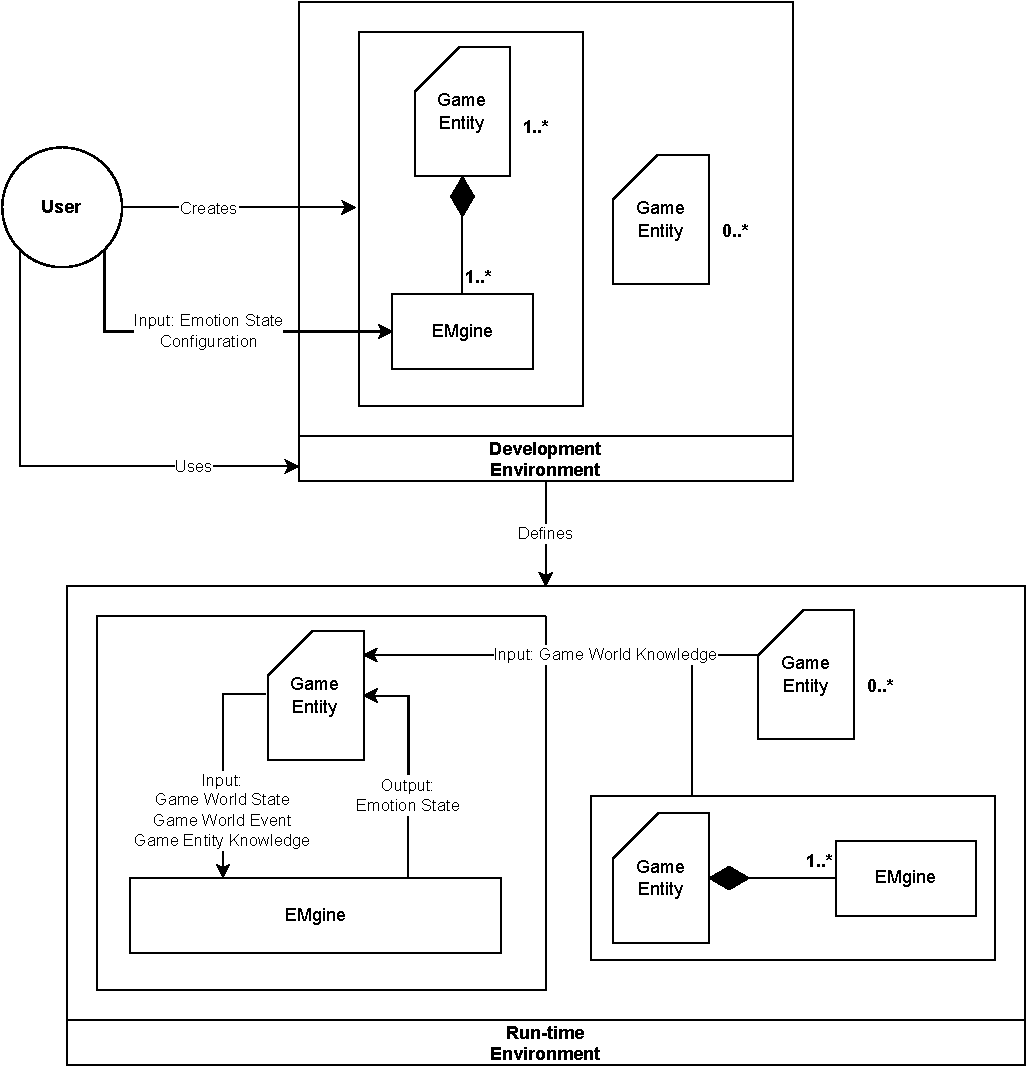
\includegraphics[width=0.9\textwidth]{figures/systemContext_Revised.pdf}
    \caption{System Context}
    \label{fig_sysContext}
\end{figure}

Within this context, each element has responsibilities to ensure that
\progname{} can function correctly:
\begin{enumerate}

    \item User (Game Designer/Developer) Responsibilities
    \begin{itemize}
        \item Associate at least one game entity with one or more \progname{}
        instances
        \item Provide functions required to evaluate \progname{}'s
        time-dependent inputs
        \item Associate \progname{} emotion types with game entity animations,
        audio, and/or behaviours
    \end{itemize}

    \item Development Environment Responsibilities
    \begin{itemize}
        \item Provide a method for interfacing with third-party systems
    \end{itemize}

    \item Run-time Environment Responsibilities
    \begin{itemize}
        \item Allow game entities to store and/or update information
        \item Allow game entities to exchange information
    \end{itemize}

    \item Game Entity Responsibilities
    \begin{itemize}
        \item Send information about events and objects in the game environment
        to one or more of their associated \progname{} instances
        \item Execute animations, audio and/or behaviours associated with
        \progname{} emotion types based on its outputs
    \end{itemize}

    \item \progname{} Responsibilities
    \begin{itemize}
        \item Detect and prevent data type mismatch, such as a string of
        characters instead of a floating point number
        \item Allow users to modify its default parameters
        \item Allow users to define new emotion types
        \item Evaluate incoming information and make corresponding updates to
        its emotion state
        \item Allow game entities to query its emotion state
    \end{itemize}

\end{enumerate}

\subsection{User Characteristics} \label{SecUserCharacteristics}
The end user of \progname{} should:
\begin{itemize}

    \item Understand how to install third-party systems in a development 
    environment

    \item Be able to read and implement APIs, understand game states, and know 
    how to design and implement agent goals

    \item A general understanding of different types of emotion and how they 
    can be expressed is an asset

\end{itemize}

\subsection{System Constraints}\label{sec_systemConstraints}
\progname{} has no known system constraints.


    \clearpage

    \section{Specific System Description}\label{sec_SpecDesc}
This section first presents the problem description, giving a high-level view 
of the problem to solve (\ref{Sec_pd}), some terminology and definitions to 
clarify models, data, and requirements (Section~\ref{sec_terms}), and goals 
that a solution must achieve (Section~\ref{sec_goals}). It then describes 
characteristics of a potential solution, including Assumptions 
(Section~\ref{sec_assumptions}), Theoretical Models 
(Section~\ref{sec_theoretical}), General and Data Definitions 
(Sections~\ref{sec_gendef} and~\ref{sec_datadef}), Data Types 
(Section~\ref{sec_typedefs}), and the Instance Models derived from these 
(Section~\ref{sec_instance}). This is followed by Constraints 
(Section~\ref{sec_DataConstraints}) and Properties of a Correct Solution 
(Section~\ref{sec_CorrectSolution}).

One section---Conceptual Models (Section~\ref{sec_conceptual})---has been added 
to the solution characteristics that is not in the SRS template in 
\cite{SmithAndLai2005} and \cite{SmithEtAl2007}. It is useful for maintaining a 
direct connection to the affective research behind the Theoretical and Instance 
Models. The Theoretical Models also differ from those in the template, focusing 
on rewriting descriptions in the Conceptual Models with more precise natural 
language. This shows what interpretation of the Conceptual Models that lead to 
their mathematical representations in the Data Types and Instance Models.

\subsection{Problem Description} \label{Sec_pd}
The purpose of \progname{} is to generate an emotion state for an entity, as 
well as store and update said emotion state with generated or given data. It 
must be done to afford users the most control over when and how \progname{} 
generates emotion with only a layperson's understanding of emotion and emotion 
processes.

\subsubsection{Terminology and  Definitions}\label{sec_terms}
The Conceptual Models (Section~\ref{sec_conceptual}) contain many definitions 
necessary for reducing ambiguity and making it easier to understand models and 
requirements. These are additional terms that do not appear in the Conceptual 
Models, but are still useful for the same reasons. \\

\noindent\textbf{Affect}: Any type of affective experience that has a
changeable, short-term state originating from the body and impacting the
mind in some way~\citep{barrett2009affect, oxfordAffect}. A general
affective state is generally identified as weaker than an emotion state. \\

\noindent\textbf{Affective Science}: The interdisciplinary study of affective 
phenomena, related processes, and its influencing 
factors~\citep[p.~xiii]{davidson2003handbook}. \\

\noindent\textbf{Appraisal Theories (Perspective)}: These theories shift the 
evaluation of the environment from its objective qualities to its relation to 
an individual's well-being~\citep[p.~86]{smith2000consequences}. They mainly 
focus on the link between cognitive processing and emotion 
elicitation~\citep[p.~354]{broekens2021emotion}. \\

\noindent\textbf{Arousal}: A short-term state of excitement or energy
expenditure~\citep{oxfordArousal}. \\

\noindent\textbf{Cognition}: ``All forms of knowing and awareness, such as
perceiving, conceiving, remembering, reasoning, judging, imagining, and problem
solving''~\citep{cognitiondef}. \\

\noindent\textbf{Core Affect}: Based on affect, ``...a state of pleasure or
displeasure with some degree of arousal''~\citep[p.~170]{barrett2009affect}.
See also \textit{Affect}. \\

\noindent\textbf{Dimensional Theories (Perspective)}: These theories can more 
easily distinguish between different emotions (\citepg{scherer2010emotion}{12}; 
\citepg{smith1985patterns}{813}) using a small number of continuous dimensions. 
They view emotion as an individual's interpretation of their current ``core 
affect''~\citep[p.~353]{broekens2021emotion} (i.e. elementary affective 
feelings). While any point in dimensional space is part of ``core 
affect''~\citep[p.~97]{lisetti2015and}, it is possible for individuals to 
verbally label points representing their subjective feeling of an 
emotion~\citep[p.~12]{scherer2010emotion}. This creates an effect of 
``plotting'' emotion categories (e.g. discrete theories) as points in the 
space. \\

\noindent\textbf{Discrete Theories (Perspective)}: These theories propose that 
innate, hard-wired circuits or programs elicit emotions 
(\citepg{ortony2021all}{41}; \citepg{scherer2021towards}{280}). One of the core 
features of these theories is the definition of distinct
emotion categories or types, like \textit{Joy} and \textit{Anger}, that are
recognizable by a set of observable features (e.g. facial expression, typical
behaviours). This ``...fits with the way we talk about emotion every
day...people automatically and effortlessly perceive emotion in themselves and
others...''~\citep[p.~47--48]{barrett2006emotions}. \\

\noindent\textbf{Emotion Expression}: An affective computing task where a CME
changes an entity's ``observable'' behaviour (e.g. facial expressions,
gestures, or movements) given an emotion state (\citepg{scherer2010emotion}{4};
\citepg{fathalla2020emotional}{2}). \\

\noindent\textbf{Emotion Generation}: An affective computing task where a CME
produces an emotion state given the current program and environment state
(\citepg{scherer2010emotion}{4}; \citepg{fathalla2020emotional}{2}). \\

\noindent\textbf{Emotion Kind}: Names given to discrete categories/types of
emotion (e.g. \textit{Joy}, \textit{Sadness}). \\

\noindent\textbf{Emotion State}: The set of values for each possible emotion
kind. \\

\noindent\textbf{Entity}: Any discrete, identifiable, and separate object that
is significant in and of themselves. \\

\noindent\textbf{``Fast, Primary Emotions''}: Hard-wired and potentially 
inaccurate responses to innate knowledge elicited by fundamental mechanisms 
(e.g. instinctual fear of pain)~\citep[p.~60--70]{picard1997affective}. \\

\noindent\textbf{Feeling}: Conscious mental representations and interpretations
of an emotional response, and follow emotions evolutionarily and experientially
(\citepg{oxfordFeelings}{184}; \citepg{scherer2000psychological}{139}).
Feelings are ill-defined from a modelling perspective, and rarely, if ever,
appear computationally. They are also, allegedly, unnecessary for understanding
emotional behaviours~\citep{fellous2004human}. \\

\noindent\textbf{Game World}: An imaginary universe in which game events  take
place~\citep{adams2014fundamentals}. They are often two or three dimensional
spaces containing characters and objects. \\

\noindent\textbf{Global Adaptational Problem}: In PES, a survival-related issue
that emotion-based behaviours evolved to address and are found in some form at
all evolutionary levels~\citep{robert1980emotion}. \\

\noindent\textbf{Gustatory}: Concerned with tasting or the sense of taste. In
CTE, this is associated with the mental process of withdrawing from toxins and
potentially infectious agents~\citep[p.~57]{oatley1992best}. In this way, it
could also be a prototype for other withdrawal-based emotions (e.g.
\textit{Hatred}, \textit{Contempt}). \\

\noindent\textbf{``Model of Self''}: In CTE, a cognitive representation of the
individual's own goals, abilities, habits, and bodies, chiefly in relation with
others~\citep[p.~195]{oatley1992best}. \\

\noindent\textbf{Mood}: Enduring, less intense, and more diffuse states than
emotions~\citep{oxfordMood}. Their presence is typically unclear to the
experiencing individual and often have a more prolonged influence on an
individual’s cognition and behaviours. \\

\noindent\textbf{Non-propositional Meaning}: In relation to communication,
signals with no symbolic structure or literal meaning of significance within a
system~\citep[p.~32]{oatley1987towards}. \\

\noindent\textbf{Personality}: Permanent or difficult to change variables that
impact affective processes~\citep{oxfordPersonality}. \\

\noindent\textbf{Propositional Meaning}: In relation to communication, signals
having a symbolic structure with a literal meaning of significance to a
system~\citep[p.~32]{oatley1987towards}. \\

\noindent\textbf{Self-Preservational}: In relation to self-preservation,
especially regarded as a basic instinct in human beings and animals, the
protection of oneself from harm or death. \\

\noindent\textbf{``Slow, Secondary Emotions''}: Sometimes called 
``cognitively-generated emotions'', these require some level of reasoning to 
elicit (e.g. learned fear of public 
speaking)~\citep[p.~60--70]{picard1997affective}. \\

\noindent\textbf{Valence}: Describes the positive or negative character of
emotions, their response components, and emotion-eliciting
stimuli~\cite{oxfordValence}. In affective science, it often appears as a
dimensional variable with positive and negative poles. Assigning valence to
an emotion depends on its context (e.g. behavioural tendencies vs. social
interactions).

\subsubsection{Physical System Description}
\progname{} does not interact with a physical system, and is not concerned with
the physical hardware that the run-time environment and its components run on
or how it generates data.

\subsubsection{Goal Statements}\label{sec_goals}
Given an entity that is associated with at least one instance of \progname{},
the entity's goals, a world state, an event that changes or could change that
world state, and optional world and/or entity knowledge, \progname{}'s goals
are:
\begin{itemize}

    \item[GS\refstepcounter{goalnum}\thegoalnum \label{G_EmotionGeneration}]
    Determining what emotion type and intensity is elicited by a change in game
    world state.

    \item[GS\refstepcounter{goalnum}\thegoalnum \label{G_EmotionDecay}]
    Determining what intensity each emotion type has when decaying emotion.

    \item[GS\refstepcounter{goalnum}\thegoalnum \label{G_UpdateEmotionState}]
    Updating stored emotion values.

    \item[GS\refstepcounter{goalnum}\thegoalnum \label{G_QueryEmotionState}]
    Allowing queries about stored emotion values.

\end{itemize}

The goal statements only describe \progname{}'s \textit{tasks}. \progname{}
also requires goals (i.e. high-level requirements) describing its target
\textit{properties} to guide the selection of its underlying emotion theories
(Section~\ref{sec_theories}). This process is needed to define the Assumptions
(Section~\ref{sec_assumptions}) and Conceptual Models
(Section~\ref{sec_conceptual}). The high-level requirements directly
incorporate some of the needs of video game designers/developers
(Section~\ref{sec:doc_stakeholder}) to improve the probability of \progname{}'s
acceptance, which the SRS incorporates in the nonfunctional requirements
(Section~\ref{sec_ReqsNF}).

The \textit{flexibility} goals are about making \progname{} adaptable so that
it can meet game designer needs~\citep[p.~30]{reilly1996believable}. The aim is
for \progname{} to be applicable to a range of game designs while avoiding
making decisions for the game developer.
\begin{enumerate}[label=RF\arabic*]
    \item\label{flexArch} Independence from an agent architecture so that
    designers can choose how to integrate \progname{} into their game
    (\citepg{loyall1997believable}{25--26};
    \citepg{rodriguez2015computational}{443};
    \citepg{broekens2016emotional}{218})

    \item\label{flexTasks} Allowing the game designer to choose which of
    \progname{}'s tasks to use, as well as when and how to use
    them (\citepg{mascarenhas2022fatima}{8:13};
    \citepg{guimaraes2022fatima}{20})

    \item\label{flexCustom} Allowing the customization or redefinition of
    \progname{}'s pre-existing configuration parameters
    (\citepg{reilly1996believable}{30}; \citepg{guimaraes2022fatima}{20})
    such as the definition of time and emotion decay rates

    \item\label{flexNew} Allowing designers to integrate new components
    into \progname{} that influence or are influenced by emotion
    (\citepg{rodriguez2015computational}{450};
    \citepg{castellanos2019mechanism}{353}), such as mood, personality,
    motivations, culture, gender, and physical state

    \item\label{flexEm} Allowing designers to choose which kinds of emotion
    \progname{} produces (i.e. which emotions an NPC can
    have)~\citep[p.~331]{hudlicka2014computational}, (e.g. \textit{Anger},
    \textit{Joy})

    \item\label{flexOut} Allowing designers to specify how to use
    \progname{}'s outputs~\citep[p.~86]{loyall1997believable}

    \item\label{flexComplex} Allow designers to use \progname{} on
    different levels of NPC
    complexity~\citep[p.~220]{broekens2016emotional}, e.g. a
    \textit{Pac-man} ghost~\citep{pacman} and a \textit{Skyrim}
    citizen~\citep{skyrim} will not have the same emotional requirements

    \item\label{flexScale} Being efficient and scalable to minimize
    \progname{}'s impact on overall game performance
    \citep[p.~42]{popescu2014gamygdala}
\end{enumerate}

The \textit{ease-of-use} goals concern the usability of \progname{} and showing
how it supports game development. These aim to make \progname{} more
user-friendly and minimize maintenance to increase its chances of adoption by
game developers.
\begin{enumerate}[label=RE\arabic*]
    \item\label{easeHide} Hiding the complexity of emotion generation so
    that game designers do not have to be knowledgeable in emotion
    psychology to use \progname{} (\citepg{reilly1996believable}{28};
    \citepg{broekens2016emotional}{220}; \citepg{guimaraes2022fatima}{5})

    \item\label{easeAPI} Providing a clear and understandable Application
    Programming Interface (API) or similar that shows how to use the
    different aspects of \progname{}~\citep[p.~218]{broekens2016emotional}

    \item\label{easeAuthor} Minimizing authorial burden as game developers
    add NPCs to their game~\citep[p.~5]{guimaraes2022fatima}

    \item\label{easeTrace} Allowing \progname{}'s outputs to be traceable
    and understandable (\citepg{loyall1997believable}{86};
    \citepg{guimaraes2022fatima}{5, 19--20})---critical for testing---by
    providing ways to view the range, intensity, and causes of emotion per
    NPC, per NPC group, and per game world
    area~\citep[p.~219--220]{broekens2016emotional}

    \item\label{easeAuto} Allowing developers the option to automate the
    storing and decaying of \progname{}'s internal emotion
    state~\citep[p.~86]{loyall1997believable}

    \item\label{easePX} Showing that \progname{} improves the player
    experience, since a sub-par design could be a detriment to the overall
    game and would not be of use to game development

    \item\label{easeNovel} Providing examples as to how \progname{} can
    create novel game experiences~\citep[p.~221]{broekens2016emotional}
\end{enumerate}

The flexibility and ease-of-use goals also imply that \progname{} \textit{must
not} depend on a particular entity embodiment or implementation because this
limits the types of entities that it could support (related to \ref{flexArch},
\ref{flexComplex}), and it \textit{must} support the generation of
\textit{fast, primary emotions} and \textit{slow, secondary
emotions}~\citep[p.~60--70]{picard1997affective} (related to \ref{flexComplex}).

\newpage

\subsection{Solution Characteristics Specification}\label{Sec_scs}

This section expresses \progname{}'s solution characteristics in mathematical
form via Data Types (Section \ref{sec_typedefs}) and Instance Models
(Section~\ref{sec_instance}), as well as underlying Assumptions
(Section~\ref{sec_assumptions}), Data Constraints
(Section~\ref{sec_DataConstraints}) and additional properties necessary for
\progname{} to be correct (Section~\ref{sec_CorrectSolution}). These components
are refinements of Theoretical Models (Section~\ref{sec_theoretical}), which
are in turn refinements of Conceptual Models (Section~\ref{sec_conceptual}).
They are necessary for understanding the Data Types and Instance Models so that
they can be verified.

\subsubsection{Emotion Theories and Models}\label{sec_theories}
All potential \progname{} solutions must be based on emotion theories and data
to improve its \textit{psychologically validity}, which is necessary for its
behaviours to be \textit{plausible}~\citep[p.~216--217]{broekens2016emotional}.
The theories that \progname{} uses must align with its overall design goals.

\progname{}'s theories are Oatley \& Johnson-Laird's Communicative Theory of
Emotion (CTE), Plutchik's Psycho-Evolutionary Synthesis (PES), and Mehrabian's
Pleasure-Arousal-Dominance Space (PAD). These were chosen from a pool of
potential candidates (Table~\ref{tab:theories}) based on their ability to
satisfy the \textit{flexibility} and \textit{ease-of-use} high-level
requirements (Section~\ref{sec_systemConstraints}). Note that these
requirements are theory-agnostic, so any emotion theory that supports them is a
reasonable choice.

The selection process follows these general steps:
\begin{enumerate}
    \item Scoping the high-level requirements as needed
    \item Scoring each candidate theory
    \item Choosing theories based on their scores
\end{enumerate}

\paragraph{Scoping}
The analysis separates \textit{Providing a clear and understandable API}
(\ref{easeAPI}) into two---Input and Output---to get a better feel for each
theory's usefulness. This is an acknowledgement that some theories are better
for emotion expression, such as Ekman \& Friesen.

The requirement for \textit{Allowing the Integration of New Components}
(\ref{flexNew}) is broad and should be scoped for the initial design of
\progname{}. New \progname{} components could be non-affective (e.g. attention)
and affective (e.g. personality) in nature. Integrating non-affective
components should be theory-agnostic, as they are part of separate components
of mind~\citep{cognitiondef}. From a software engineering perspective, one
could view the mind as a system with distinct, interacting subsystems. Modular
interfaces that control interactions between \progname{}---as the affective
subsystem---and components from other subsystems would support this concept,
while also maintaining \progname{}'s requirements for \textit{Independence from
an Agent Architecture} (\ref{flexArch}) and \textit{Allowing Developers to
Specify How to Use Outputs} (\ref{flexOut}). Integrating other affective
components would depend on \progname{} and its foundational theories. One would
be limited to only those components that can be represented in terms of the
emotions or other types of affect that have been connected to them.

This requirements analysis focuses on three other types of affect: core affect,
mood, and personality. Of these, it prioritizes personality because it is
necessary for creating the consistent and coherent agent behaviours that
influence believability (\citepg{reilly1996believable}{26};
\citepg{loyall1997believable}{19}; \citepg{ortony2002making}{203}).

Finally, the \textit{Minimizing authorial burden} requirement
(\ref{easeAuthor}) is excluded from the analysis. This is due to its focus on
helping game developers manage the creation of an increasing NPC population,
rather than the functionality of \progname{} itself.

\begin{table}[!tbh]
    \renewcommand{\arraystretch}{1.2}
    \centering
    \caption{Theories Analysed}
    \label{tab:theories}
    \begin{tabular}{P{0.2\columnwidth}P{0.65\columnwidth}}
        \toprule
        \textbf{Perspective} & \textbf{Theories} \\
        \midrule

        \rowcolor[gray]{0.9}Discrete & Ekman \& Friesen (Ek.), Izard (Iz.),
        Plutchik (Plu.) \\

        Dimensional & Valence-Arousal (V-A), PAD Space (PAD) \\

        \rowcolor[gray]{0.9}Appraisal & Frijda (Frj.), Lazarus (Laz.), Scherer
        (Sch.), Roseman (Ros.), Ortony, Clore, and Collins (OCC), Smith \&
        Kirby (S \& K), Oatley \& Johnson-Laird (O \& JL) \\

        \bottomrule
    \end{tabular}
\end{table}

\paragraph{Scoring} Each theory has a set of notes made during their
examination, guided by individual high-level requirements. After reviewing the
notes, each theory is assigned a \textit{score} describing its relative
``suitability'' for that requirement (Table~\ref{tab:scoring}). This step is
somewhat subjective because a judgement is made without true objective measures
or methods. The notes are in Appendix~\ref{chapter:reqsTheoryNotes}.

\progname{}'s high-level requirements are divided into two sets:
\textit{system-level}, which applies to \progname{} as a whole
(Tables~\ref{tab:theory-req-sys-summary-flexibility} and
\ref{tab:theory-req-sys-summary-easeofuse}), and \textit{component-level} for
requirements that only apply to specific pieces of \progname{}
(Tables~\ref{tab:theory-req-comp-summary-flexibility} and
\ref{tab:theory-req-comp-summary-easeofuse}). Only appraisal theories are
assigned categories for component-level requirements because they concern
process-related elements that discrete and dimensional theories do not address.
Each theory has unique elements, which might make it better or worse suited for
a particular requirement. These are noted in the analysis. However, is not
unusual for theories from the same perspective to satisfy a requirement equally
well. In these cases, the theories are treated as a collective unit when
examining the requirement.
Tables~\ref{tab:theory-req-sys-summary-flexibility},
\ref{tab:theory-req-sys-summary-easeofuse},
\ref{tab:theory-req-comp-summary-flexibility}, and
\ref{tab:theory-req-comp-summary-easeofuse} summarize the scores for each
theory and requirement.

\begin{table}[!h]
    \renewcommand{\arraystretch}{1.2}
    \centering
    \caption{Summary of Scoring Categories}
    \label{tab:scoring}
    \begin{tabular}{ccP{0.65\columnwidth}}
        \toprule
        \textbf{Score Category} & \textbf{Symbol} & \textbf{Definition} \\

        \midrule

        \rowcolor[gray]{0.9}\textit{Strong} & \strong & The theory
        appears to satisfy the requirement in a clear, understandable way and
        is likely to aid in \progname{}'s usability
        \\

        \textit{Good} & \good & The theory appears to satisfy the requirement
        and is somewhat defined \\

        \rowcolor[gray]{0.9}\textit{Weak} & \weak & The theory
        describes ways that \textit{could} satisfy the requirement, but it is
        not fully defined or could make \progname{} harder to use \\

        \textit{Disqualified} & \disqualified & The theory does not seem likely
        to be able to satisfy this requirement, or it violates other
        requirements when it can (including psychological validity) \\

        \bottomrule

    \end{tabular}
\end{table}

\begin{table}[!tbh]
    \renewcommand{\arraystretch}{1.2}
    \centering
    \caption[Support for System-Level Flexibility High-Level
    Requirements]{Support for System-Level \textbf{Flexibility} High-Level
        Requirements}
    \label{tab:theory-req-sys-summary-flexibility}
    \footnotesize
    \begin{threeparttable}
        \begin{tabular}{@{}cP{0.13\linewidth}cccccccccccc@{}}

            \toprule
            \multicolumn{2}{c}{} & \hd{\textbf{Ek.}} &
            \hd{\textbf{Iz.}} & \hd{\textbf{Plu.}} & \hd{\textbf{V-A}}
            & \hd{\textbf{PAD}} & \hd{\textbf{Frj.}} &
            \hd{\textbf{Laz.}\textsuperscript{\footnotesize\textpmhg{\Hi}}} &
            \hd{\textbf{Sch.}} & \hd{\textbf{Ros.}} &
            \hd{\textbf{OCC}} & \hd{\textbf{S \& K}} & \hd{\textbf{O \&
                    JL}} \\
            \midrule

            \rowcolor[gray]{0.9}\ref{flexArch} & \textit{Independence
                from an Agent Architecture} & {\normalsize\good} &
            {\normalsize\good} & {\normalsize\good} & {\normalsize\good} &
            {\normalsize\good} & {\normalsize\strong} & {\normalsize\good} &
            \disqualified & {\normalsize\good} & {\normalsize\strong} &
            {\normalsize\strong} & {\normalsize\strong} \\

            \ref{flexNew} & \textit{Allowing the Integration of
                Components}{\large\textpmhg{\Hl}} & {\normalsize\weak} &
            {\normalsize\weak}\textsuperscript{\normalsize\Moon} &
            {\normalsize\good}\textsuperscript{\normalsize\Moon} &
            {\normalsize\strong}\textsuperscript{\large\Jupiter} &
            {\normalsize\strong}\textsuperscript{\large\Jupiter} &
            {\normalsize\strong} & {\normalsize\weak} & {\normalsize\weak} &
            {\normalsize\weak} & {\normalsize\strong} & {\normalsize\weak} &
            {\normalsize\strong} \\

            \rowcolor[gray]{0.9}\ref{flexEm} & \textit{Choosing NPC
                Emotions} & {\normalsize\weak} & \disqualified &
            {\normalsize\strong} & {\normalsize\weak} & {\normalsize\good} &
            {\normalsize\weak} & {\normalsize\weak} & {\normalsize\good} &
            {\normalsize\good} & {\normalsize\good} & {\normalsize\weak} &
            {\normalsize\strong} \\

            \ref{flexOut} & \textit{Allowing Developers to Specify How to Use
                CME Outputs} & {\normalsize\good} & {\normalsize\good} &
            {\normalsize\good} & {\normalsize\strong} & {\normalsize\strong} &
            {\normalsize\strong} & {\normalsize\strong} & {\normalsize\strong} &
            {\normalsize\strong} & {\normalsize\strong} & {\normalsize\strong}
            & {\normalsize\strong} \\

            \rowcolor[gray]{0.9}\ref{flexComplex} & \textit{Ability to
                Operate on Different Levels of NPC Complexity} &
                {\normalsize\good}
            & {\normalsize\good} & {\normalsize\good} & {\normalsize\weak} &
            {\normalsize\weak} & {\normalsize\weak} & {\normalsize\strong} &
            {\normalsize\strong} & {\normalsize\good} & {\normalsize\good} &
            {\normalsize\strong} & {\normalsize\good} \\

            \ref{flexScale} & \textit{Be Efficient and Scalable} &
            {\normalsize\good} & {\normalsize\good} & {\normalsize\good} &
            {\normalsize\weak} & {\normalsize\weak} &
            {\normalsize\good}\textsuperscript{\large\Pluto} &
            {\normalsize\strong} & {\normalsize\good} & {\normalsize\weak} &
            {\normalsize\good} & {\normalsize\strong} & {\normalsize\strong} \\

            \hline\bottomrule
        \end{tabular}
        \begin{tablenotes}

            \footnotesize
            \vspace*{2mm}

            \item \textit{See Table~\ref{tab:scoring} for score category
                descriptions.}

            \item {\small\textpmhg{\Hi}} \textit{Excludes the
                \textit{Coping Process} because it is part of action
                generation.}

            \item {\Large\textpmhg{\Hl}} \textit{Strictly focusing on
                core affect, mood, and personality.}

            \item {\normalsize\Moon} \textit{Natively supports integration
                with Personality.}

            \item {\Large\Jupiter} \textit{Personality integration
                based on the Five Factor Model (OCEAN).}

            \item {\Large\Pluto} \textit{Might improve if some factors
                are not necessary for implementation scope.}

        \end{tablenotes}
    \end{threeparttable}%
\end{table}

\begin{table}[!tbh]
    \renewcommand{\arraystretch}{1.2}
    \centering
    \caption[Support for System-Level Ease-of-Use High-Level
    Requirements]{Support for System-Level \textbf{Ease-of-Use}
        High-Level Requirements}
    \label{tab:theory-req-sys-summary-easeofuse}
    \footnotesize
    \begin{threeparttable}
        \begin{tabular}{@{}cP{0.21\linewidth}cccccccccccc@{}}

            \toprule
            \multicolumn{2}{c}{} & \hd{\textbf{Ek.}} &
            \hd{\textbf{Iz.}} & \hd{\textbf{Plu.}} &
            \hd{\textbf{V-A}} & \hd{\textbf{PAD}} &
            \hd{\textbf{Frj.}} &
            \hd{\textbf{Laz.}\textsuperscript{\footnotesize\textpmhg{\Hi}}} &
            \hd{\textbf{Sch.}} & \hd{\textbf{Ros.}} &
            \hd{\textbf{OCC}} & \hd{\textbf{S \& K}} &
            \hd{\textbf{O \& JL}} \\
            \midrule

            \rowcolor[gray]{0.9}\ref{easeAPI} & \textit{Having a Clear
                API (Output)} & {\normalsize\strong} & {\normalsize\weak} &
            {\normalsize\good} & {\normalsize\weak} & {\normalsize\weak} &
            {\normalsize\good} & {\normalsize\strong} & {\normalsize\weak} &
            {\normalsize\strong} & {\normalsize\good} & {\normalsize\strong} &
            {\normalsize\strong} \\

            \ref{easePX} & \textit{Showing that Emotions Improve the Player
                Experience} & {\normalsize\good} & {\normalsize\good} &
            {\normalsize\good} & {\normalsize\good} & {\normalsize\good} &
            {\normalsize\good} & {\normalsize\good} & {\normalsize\strong} &
            {\normalsize\good} & {\normalsize\weak} & {\normalsize\good} &
            {\normalsize\good} \\

            \rowcolor[gray]{0.9}\ref{easeNovel} & \textit{Providing
                Examples of Novel Game Experiences} & {\normalsize\weak} &
            {\normalsize\weak} & {\normalsize\weak} & {\normalsize\good} &
            {\normalsize\good} & {\normalsize\good} & {\normalsize\good} &
            {\normalsize\good} & {\normalsize\good} & {\normalsize\good} &
            {\normalsize\good} & {\normalsize\good} \\

            \hline\bottomrule
        \end{tabular}
        \begin{tablenotes}

            \footnotesize
            \vspace*{2mm}

            \item \textit{See Table~\ref{tab:scoring} for score category
                descriptions.}

            \item {\small\textpmhg{\Hi}} \textit{Excludes the
                \textit{Coping Process} because it is part of action
                generation.}

        \end{tablenotes}
    \end{threeparttable}%
\end{table}

\begin{table}[!tbh]
    \renewcommand{\arraystretch}{1.2}
    \centering
    \caption[Support for Component-Level Flexibility High-Level
    Requirements]{Support for Component-Level \textbf{Flexibility}
        High-Level Requirements}
    \label{tab:theory-req-comp-summary-flexibility}
    \footnotesize
    \begin{threeparttable}
        \begin{tabular}{@{}cP{0.25\linewidth}ccccccc@{}}

            \toprule
            \multicolumn{2}{c}{} & \hd{\textbf{Frj.}} &
            \hd{\textbf{Laz.}\textsuperscript{\footnotesize\textpmhg{\Hi}}} &
            \hd{\textbf{Sch.}} & \hd{\textbf{Ros.}} &
            \hd{\textbf{OCC}} & \hd{\textbf{S \& K}} & \hd{\textbf{O \&
                    JL}} \\
            \midrule

            \rowcolor[gray]{0.9}\ref{flexTasks} & \textit{Choosing
                Which Tasks to Use} & {\normalsize\weak} & {\normalsize\weak} &
            {\normalsize\strong} & \disqualified & {\normalsize\good} &
            {\normalsize\good} & {\normalsize\good} \\

            \ref{flexCustom} & \textit{Customization of Existing Task
                Parameters} & {\normalsize\strong} & \disqualified &
            {\normalsize\good} & \disqualified & {\normalsize\good} &
            {\normalsize\good} & {\normalsize\good} \\

            \hline\bottomrule
        \end{tabular}
        \begin{tablenotes}

            \footnotesize
            \vspace*{2mm}

            \item \textit{See Table~\ref{tab:scoring} for score category
                descriptions.}

            \item {\small\textpmhg{\Hi}} \textit{Excludes the
                \textit{Coping Process} because it is part of action
                generation.}

        \end{tablenotes}
    \end{threeparttable}%
\end{table}

\begin{table}[!tbh]
    \renewcommand{\arraystretch}{1.2}
    \centering
    \caption[Support for Component-Level Ease-of-Use High-Level
    Requirements]{Support for Component-Level \textbf{Ease-of-Use}
        High-Level Requirements}
    \label{tab:theory-req-comp-summary-easeofuse}
    \footnotesize
    \begin{threeparttable}
        \begin{tabular}{@{}cP{0.25\linewidth}ccccccc@{}}

            \toprule
            \multicolumn{2}{c}{} & \hd{\textbf{Frj.}} &
            \hd{\textbf{Laz.}\textsuperscript{\footnotesize\textpmhg{\Hi}}}
            & \hd{\textbf{Sch.}} & \hd{\textbf{Ros.}} &
            \hd{\textbf{OCC}} & \hd{\textbf{S \& K}} &
            \hd{\textbf{O \& JL}} \\
            \midrule

            \rowcolor[gray]{0.9}\ref{easeHide} & \textit{Hiding the
                Complexity of Emotion Generation} & {\normalsize\strong} &
            {\normalsize\strong} & {\normalsize\strong} & {\normalsize\good} &
            {\normalsize\good} & {\normalsize\good} & {\normalsize\good} \\

            \ref{easeAPI} & \textit{Having a Clear API (Input)} &
            {\normalsize\good} & {\normalsize\disqualified} &
            {\normalsize\good} & {\normalsize\good} & {\normalsize\weak} &
            {\normalsize\good} & {\normalsize\strong} \\

            \rowcolor[gray]{0.9}\ref{easeTrace} & \textit{Traceable
                CME Outputs} & {\normalsize\strong} & {\normalsize\strong} &
            {\normalsize\weak} & {\normalsize\strong} & {\normalsize\strong} &
            {\normalsize\strong} & {\normalsize\strong} \\

            \ref{easeAuto} & \textit{Allowing the Automatic Storage and Decay
                of the Emotion State} & {\normalsize\good} & {\normalsize\good}
                &
            {\normalsize\good} & {\normalsize\disqualified} &
            {\normalsize\good} & {\normalsize\good} & {\normalsize\good} \\

            \hline\bottomrule
        \end{tabular}
        \begin{tablenotes}

            \footnotesize
            \vspace*{2mm}

            \item \textit{See Table~\ref{tab:scoring} for score category
                descriptions.}

            \item {\small\textpmhg{\Hi}} \textit{Excludes the
                \textit{Coping Process} because it is part of action
                generation.}

        \end{tablenotes}
    \end{threeparttable}%
\end{table}

\paragraph{Choosing Theories} \progname{} prioritizes \ref{flexArch},
\ref{flexOut}, \ref{flexComplex}, \ref{flexScale}, \ref{easeHide},
\ref{easeAPI}, and \ref{easeTrace} because it is unlikely that developers will
adopt \progname{} without them. The remaining requirements offer more options
to tailor it to different game designs (\ref{flexTasks}, \ref{flexCustom},
\ref{easeAuto}) and/or could be satisfied as an extension later on
(\ref{flexNew}, \ref{flexEm}, \ref{easePX}, \ref{easeNovel}).

Theories are \textit{not} immediately discounted if they cannot satisfy a
requirement (i.e. given score is \textit{Disqualified}). They might be
extremely strong in other areas. Instead, the coverage achieved by the
\textit{set} of chosen theories must satisfy all requirements. This allows
\progname{} to take advantage of the strengths of different theories while also
compensating for their weaknesses. \progname{} uses one theory from each of the
discrete, dimensional, and appraisal perspectives to take advantage of each
perspective's strengths and mitigate its weaknesses.

The discrete and dimensional theories cannot satisfy the need for
\textit{cognitively generated/slow, secondary emotions}
(Section~\ref{sec_systemConstraints}). This means that \progname{} must use at
least one appraisal theory. It is also known that the discrete theories can
best satisfy the need for \textit{fast, primary emotions}. There is no reason
to limit the number of theories in \progname{}'s design, as the added
complexity would be internal to \progname{} (otherwise it would conflict with
\ref{easeHide}). Therefore, \progname{} must use at least one appraisal and one
discrete theory.

\progname{} also uses a dimensional theory because they are especially suitable
for representing different types of affect and their interactions in a common
space (\ref{flexNew}) and afford more control over what emotions could ``do''
in an NPC (\ref{flexOut}). The additional design freedom afforded to game
developers, including a dimensional theory could increase \progname{}'s overall
applicability.
\begin{itemize}

    \item \textbf{Appraisal Theory: Oatley \& Johnson-Laird} \\
    Three theories have \textit{Disqualified} scores: Lazarus, Scherer, and
    Roseman. Roseman has an ill-defined emotion elicitation process compared to
    the others, so \progname{} should not use it. Both Lazarus and Scherer are
    \textit{Disqualified} for a priority requirement (\ref{easeAPI} (Input) and
    \ref{flexArch} respectively), so \progname{} should not use them either. Of
    the remaining theories, Oatley \& Johnson-Laird seems the most promising.
    It has only \textit{Good} or \textit{Strong} scores for all requirements,
    and all but one priority requirement (\ref{easeHide}) has a \textit{Strong}
    score.

    \item \textbf{Discrete Theory: Plutchik} \\
    The discrete theories vary in score for only three requirements:
    \ref{flexNew}, \ref{flexEm}, and \ref{easeAPI} (Output). \progname{} should
    not use Izard because it is \textit{Disqualified} for one requirement
    (\ref{flexEm}) and has no \textit{Strong} scores. Plutchik has a better
    overall score distribution compared to Ekman \& Friesen (7 \textit{Good}
    scores to 5, and the same number of \textit{Disqualified} and
    \textit{Strong} scores) and to better support \ref{flexEm}. Oatley \&
    Johnson-Laird already has a \textit{Strong} score for \ref{easeAPI}
    (Output), so the overall design benefits more from Plutchik than Ekman \&
    Friesen.

    \item \textbf{Dimensional Theory: PAD Space} \\
    V-A and PAD Space have identical scores, except for
    one---\ref{flexEm}---which PAD Space scores higher on. Therefore, I chose
    to use PAD Space for \progname{}. If needed, V-A space can be constructed
    in PAD space due to their overlapping dimensions
    (Table~\ref{tab:affectiveDimensions}).

\end{itemize}

\begin{table}[!tbh]
    \renewcommand{\arraystretch}{1.2}
    \centering
    \caption{Comparison of Dimensions in Dimensional Theories}
    \label{tab:affectiveDimensions}
    \begin{tabular}{lcc}
        \toprule
        \textbf{Dimension} &
        {\begin{tabular}[c]{@{}c@{}}\textbf{Valence-Arousal} \\
                (\textbf{V-A})\end{tabular}} &
        {\begin{tabular}[c]{@{}c@{}}\textbf{PAD} \\
                \textbf{\citep{mehrabian1996pleasure}}\end{tabular}} \\ \hline

        \rowcolor[gray]{0.9}Pleasure/Valence & \checkmark &
        \checkmark \\

        Arousal & \checkmark & \checkmark \\

        \rowcolor[gray]{0.9}Dominance &  & \checkmark \\
        \hline\bottomrule
    \end{tabular}
\end{table}

\afterpage{\clearpage}\newpage % Forces tables to appear before starting new
                               % section

\subsubsection{Assumptions}\label{sec_assumptions}
This section helps formalize the original problem to aid the development of
types, models, and definitions by filling in the ambiguous and missing
information. The numbers given in the square brackets refer to where the
assumption appears: Theoretical Model [T], General Definition [GD], Data
Definition [DD], Data Type [TY], Instance Model [IM], or Likely Change [LC]. If
there are no square brackets next to an assumption, it is generally applicable.

The Conceptual Models (Section~\ref{sec_conceptual}) have no related
assumptions because they are taken from primary sources, with no attempts at
elaboration or disambiguation.

\begin{itemize}

    \item[A\refstepcounter{assumpnum}\theassumpnum \label{A_TotalFunctions}:]
    All functions are \textit{total} unless otherwise stated.

    \item[A\refstepcounter{assumpnum}\theassumpnum \label{A_formal}:]
    Words describing concepts in conceptual models do not necessarily reflect
    how they are represented in a formal context.

    \item[A\refstepcounter{assumpnum}\theassumpnum \label{A_Cognition}:]
    \textit{Cognition} refers to the representation and transformation of
    knowledge, which might not be concious~\citep[p.~30]{oatley1987towards}.

    \item[A\refstepcounter{assumpnum}\theassumpnum \label{A_Modular}:]
    The human cognitive system is modular and
    asynchronous~\citep[p.~31]{oatley1987towards}.

    \item[A\refstepcounter{assumpnum}\theassumpnum
    \label{A_Subgoal}:] Each action and/or event that moves an entity towards
    its goal is a ``sub-goal'' [\tref{T_CalculateEmotionGP},
    \lcref{LC_Subgoal}].

    \item[A\refstepcounter{assumpnum}\theassumpnum
    \label{A_Goal2Emotion}:] A goal can elicit multiple emotions simultaneously
    [\tref{T_CalculateEmotionGP}, \lcref{LC_Goal2Emotion}].

    \item[A\refstepcounter{assumpnum}\theassumpnum
    \label{A_OneState}:] An entity is in exactly one emotion state at any given
    time [\tref{T_CalculateEmotionGP}].

    \item[A\refstepcounter{assumpnum}\theassumpnum
    \label{A_EmotionTypeIntensity}:] Emotion type and intensity do not have to
    be calculated together [\tref{T_CalculateEmotionGP},
    \lcref{LC_EmotionTypeIntensity}].

    \item[A\refstepcounter{assumpnum}\theassumpnum \label{A_AppraisalProcess}:]
    Different appraisal processes can elicit different emotions
    [\tref{T_CalculateEmotionGP}].

    \item[A\refstepcounter{assumpnum}\theassumpnum \label{A_Goal2Intensity}:]
    For CTE-based emotion kinds, emotion intensity is related to the degree
    that something impacts a goal and/or plan
    [\tref{T_CalculateEmotionIntensity}, \lcref{LC_Goal2Intensity}].

    \item[A\refstepcounter{assumpnum}\theassumpnum \label{A_CTE2PES}:]
    Emotions with the same or synonymous names in CTE and PES represent the
    same concept [\tref{T_CalculateEmotionGP}].

    \item[A\refstepcounter{assumpnum}\theassumpnum \label{A_Acceptance}:]
    \textit{Acceptance} is a ``complex'' emotion based on \textit{Joy}
    [\tref{T_CalculateEmotionAcceptance}].

    \item[A\refstepcounter{assumpnum}\theassumpnum \label{A_Interest}:]
    \textit{Interest} is related to the amount of time an entity spends
    focusing on the same thing [\tref{T_CalculateEmotionInterest},
    \lcref{LC_Interest}].

    \item[A\refstepcounter{assumpnum}\theassumpnum \label{A_Surprise}:]
    \textit{Surprise} is related to event probability
    [\tref{T_CalculateEmotionSurprise}].

     \item[A\refstepcounter{assumpnum}\theassumpnum \label{A_DecaySpeed}:]
     Emotion decays more quickly the farther it is from the ``equilibrium''
     state [\tref{T_DecayEmotionState}, \lcref{LC_DecaySpeed}].

     \item[A\refstepcounter{assumpnum}\theassumpnum \label{A_Equilibrium}:]
     Each emotion kind can have its own ``equilibrium'' value
     [\tref{T_DecayEmotionState}, \lcref{LC_Equilibrium}].

     \item[A\refstepcounter{assumpnum}\theassumpnum \label{A_DecayRate}:]
     Each emotion kind in a state can decay at its own rate
     [\tref{T_DecayEmotionState}, \lcref{LC_DecayRate}].

    \item[A\refstepcounter{assumpnum}\theassumpnum \label{A_DecayUnique}:]
    Decay rates and equilibrium values can vary between entities
    [\tref{T_DecayEmotionState}].

    \item[A\refstepcounter{assumpnum}\theassumpnum \label{A_OnePADPoint}:]
    An emotion state represents a single point in PAD Space
    [\tref{T_GetEmotionStatePAD}].

    \item[A\refstepcounter{assumpnum}\theassumpnum \label{A_EmotionTerms}:]
    Laypeople that judged emotion terms in one of PES and PAD would find that
    terms used in the other theory would have identical or nearly identical
    meanings [\tref{T_GetEmotionStatePAD}, \lcref{LC_EmotionTerms}].

    \textbf{Reasoning} This is derived from published, independently run
    empirical studies by Plutchik (PES) and Mehrabian (PAD) where they were
    evaluating their own affective models. For this study on emotion language,
    Plutchik created a list of 145 emotion terms and asked participants judged
    how ``similar'' the terms are~\citep[p.~159, 168--170]{robert1980emotion}.
    Terms were then assigned angular placements on a circumplex based on their
    relative ``similarity'' to each other. Mehrabian asked participants to
    judge the contribution of each dimension---\textit{pleasure},
    \textit{arousal}, and \textit{dominance}---in the experiences described by
    151 terms from which it derived statistical mean and standard deviation
    values~\citep[p.~39--45]{mehrabian1980basic}. Reports about the
    participants in these studies suggest that they were:
    \begin{itemize}

        \item Likely in the same age group (university undergraduates, college
        and graduate students), and

        \item Likely had an North American cultural perspective (studies done
        in the United States).

    \end{itemize}

    The publication dates (1980) further suggest that Plutchik and Mehrabian
    likely conducted their studies around the same time frame. Taken together,
    this implies that the laypeople in these studies shared common temporal and
    cultural experiences that would have influenced their interpretation of
    natural language terms.

    \item[A\refstepcounter{assumpnum}\theassumpnum \label{A_PADStats}:] The
    number of ratings and standard deviation do not affect an emotion term's
    mean values for \textit{pleasure}, \textit{arousal}, and \textit{dominance}
    [\tref{T_GetEmotionStatePAD}, \lcref{LC_PADStats}].

    \item[A\refstepcounter{assumpnum}\theassumpnum
    \label{A_ContinuousIntensity}:] Emotion intensities can be continuous
    values [\tyref{TY_EmotionIntensity}].

    \item[A\refstepcounter{assumpnum}\theassumpnum
    \label{A_RealIntensityChanges}:] Emotion intensities changes can be
    positive or negative [\tyref{TY_DeltaIntensity}].

    \item[A\refstepcounter{assumpnum}\theassumpnum \label{A_PositiveIntensity}:]
    In PES, all emotion state intensities are zero (0) in the state of ``deep
    sleep'' because ``deep sleep'' implies that the entity lost
    consciousness~\citep[p.~1--2]{mondino2021definitions} and is not
    experiencing emotion at all. [\tyref{TY_EmotionIntensity},
    \tyref{TY_EmotionDecayState}, \lcref{LC_PositiveIntensity}].

    \item[A\refstepcounter{assumpnum}\theassumpnum \label{A_EmotionPairs}:] In
    PES, the state of ``deep sleep'' implies that emotion type pairs are not
    coupled [\tyref{TY_EmotionKind}, \tyref{TY_EmotionState},
    \lcref{LC_EmotionPairs}].

    \item[A\refstepcounter{assumpnum}\theassumpnum \label{A_LimitIntensity}:]
    Emotion intensities are finite [\tyref{TY_EmotionState}].

    \item[A\refstepcounter{assumpnum}\theassumpnum \label{A_Events}:]
    The environment can be represented by variables and events are changes in
    those variables [\tyref{TY_WorldState}, \tyref{TY_WorldStateChange}].

    \item[A\refstepcounter{assumpnum}\theassumpnum \label{A_CostFunction}:]
    There is an external function $\mathtt{Cost} : \plantype \rightarrow
    \mathbb{R}$ that evaluates the ``cost'' of the plan such that low costs are
    desirable [\iref{IM_ElicitAnger}, \iref{IM_AngerIntensity}].

    \item[A\refstepcounter{assumpnum}\theassumpnum \label{A_CausedByFunction}:]
    There is an external function $\mathtt{CausedBy} : \worldstatechangetype
    \times A \rightarrow \mathbb{B}$ evaluates event causality, returning
    $\True$ if the entity believes that $A$ is responsible for causing an event
    [\iref{IM_CalculateEmotionAcceptanceElicit}].

    \item[A\refstepcounter{assumpnum}\theassumpnum
    \label{A_EventProbabilityFunction}:]
    There is an external function of that evaluates an event's probability,
    which \textit{depends on} the previous WSV because what is ``expected'' and
    ``unexpected'' depends on defined preconditions (e.g. water falling on
    someone is unexpected on a sunny day bt not on a rainy one). This model
    assumes that there are exactly two outcomes for any given event---either it
    happens or it does not. This is for
    simplicity~\citep[p.~56]{reisenzein2019cognitive} and an assumption that
    users will want more control over entity reactions in complex scenarios.
    [\iref{IM_CalculateEmotionSurpriseElicit}].

    \item[A\refstepcounter{assumpnum}\theassumpnum \label{A_DistFunction}:]
    There is an external function $\mathtt{Dist} : \worldstatetype \times
    \worldstatetype \rightarrow \statedistancetype$ that evaluates the distance
    between two world states [\iref{IM_SadnessIntensity}].

    \item[A\refstepcounter{assumpnum}\theassumpnum
    \label{A_MaxGoalImportanceFunction}:] There is an external user-defined
    value $m_G$ representing the maximum value that goal importance can be
    [\iref{IM_SadnessIntensity}].

\end{itemize}

\newpage

\subsubsection{Conceptual Models}\label{sec_conceptual}

This section focuses on descriptions from primary sources that \progname{} is
based on, included for transparency to ensure a direct connection to the
original material. The $13$ models are grouped by concern:
\begin{enumerate}

    \item Emotion structure and types [\cref{C_Emotion},
    \cref{C_EmotionStruct}, \cref{C_ComplexEmotion},
    \cref{C_ComplexEmotions-CTE}, \cref{C_PAD}]

    \item Emotion generation, intensity, and decay [\cref{C_Appraisal-CTE},
    \cref{C_EmOther}, \cref{C_EmIntensity-CTE}, \cref{C_EmDecay}]

    \item Knowledge necessary for generating emotion via PES and CTE
    [\cref{C_Goals}, \cref{C_Plans}, \cref{C_Relation-CTE}, \cref{C_Attention}]

\end{enumerate}

~\newline\noindent
\begin{minipage}{\textwidth}
    \renewcommand*{\arraystretch}{1.5}
    \begin{tabular}{| p{\colAwidth}  p{\colBwidth}|}
        \hline
        \rowcolor[gray]{0.9}
        \bf C\refstepcounter{conceptnum}\theconceptnum \label{C_Emotion} & \bf
        Emotion \\\hline
    \end{tabular}
\end{minipage}

\paragraph{Description} An emotion is a short-term affective state representing
the coordinated physiological and behavioural response of the brain and body to
events that an organism perceives as relevant (e.g. it impacts their goals
(\cref{C_Goals})).

Some researchers hypothesize that each emotion has a \textit{signature}
representing the coordinated response pattern it typically causes, including:
behavioural and expressional characteristics; somatic and neurophysiological
factors that prepare the body for action; cognitive and interpretive
evaluations that give rise to the emotion; and experiential and subjective
qualities unique to an individual. Elements of the signature can be innate or
learned.

Emotion is also characterized by its high intensity relative to other types of
affect, its tendency to come and go quickly, its association with a specific
triggering event, object, or person, and clear cognitive contents.

CTE states that emotions do not always require cognition, and they do not have
a internal symbolic structure that is significant to the system (i.e.
non-propositional signals). The signals propagate through the system on a
global level, setting and maintaining the system in a mode (emotion ``mode'').
\\\hrule

\paragraph{Source} \citet[p.~4]{jeon2017emotions},
\citet[p.~138--140]{scherer2000psychological},
\citet[p.~349--350]{broekens2021emotion}, \citet[p.~249]{frijda1986emotions},
\citet[p.~121]{smith2001toward}, \citet[p.~133]{hudlicka2019modeling},
\citet[p.~108]{scherer2001appraisalB}, \citet[p.~6]{carlson1992psychology},
\cite{oatley1987towards}

\paragraph{Depends On} \cref{C_Goals}

\paragraph{Ref. By} \cref{C_EmIntensity-CTE}, \cref{C_EmDecay},
\tyref{TY_EmotionState}, \tyref{TY_Emotion} \\\hrule\vspace{0.5mm}\hrule

~\newline

\noindent
\begin{minipage}{\textwidth}
    \renewcommand*{\arraystretch}{1.5}
    \begin{tabular}{| p{\colAwidth}  p{\colBwidth}|}
        \hline
        \rowcolor[gray]{0.9}
        \bf C\refstepcounter{conceptnum}\theconceptnum \label{C_EmotionStruct}
        &
        \bf Emotion Structure (PES) \\\hline
    \end{tabular}
\end{minipage}

\paragraph{Description} PES organizes its eight emotion kinds---\textit{Fear},
\textit{Anger}, \textit{Sadness}, \textit{Joy}, \textit{Interest},
\textit{Surprise}, \textit{Disgust}, and \textit{Acceptance}---into a cone
(Figure~\ref{fig_emotionsolid}).

The emotion types are arranged on a circular plane based on their relative
similarity as determined from empirically gathered responses. In this way,
emotions considered the most dissimilar appear on opposite sides of the plane.
The vertical axis of the solid represents emotional intensity, with the most
intense emotions at the top and a state of ``deep sleep'' at the bottom point.
The cone shape implies that the differences between the emotions becomes less
distinct at low intensities.

\begin{figure}[H]
    \centering
    \begin{subfigure}[c]{0.55\textwidth}
        \centering

        $\vcenter{\hbox{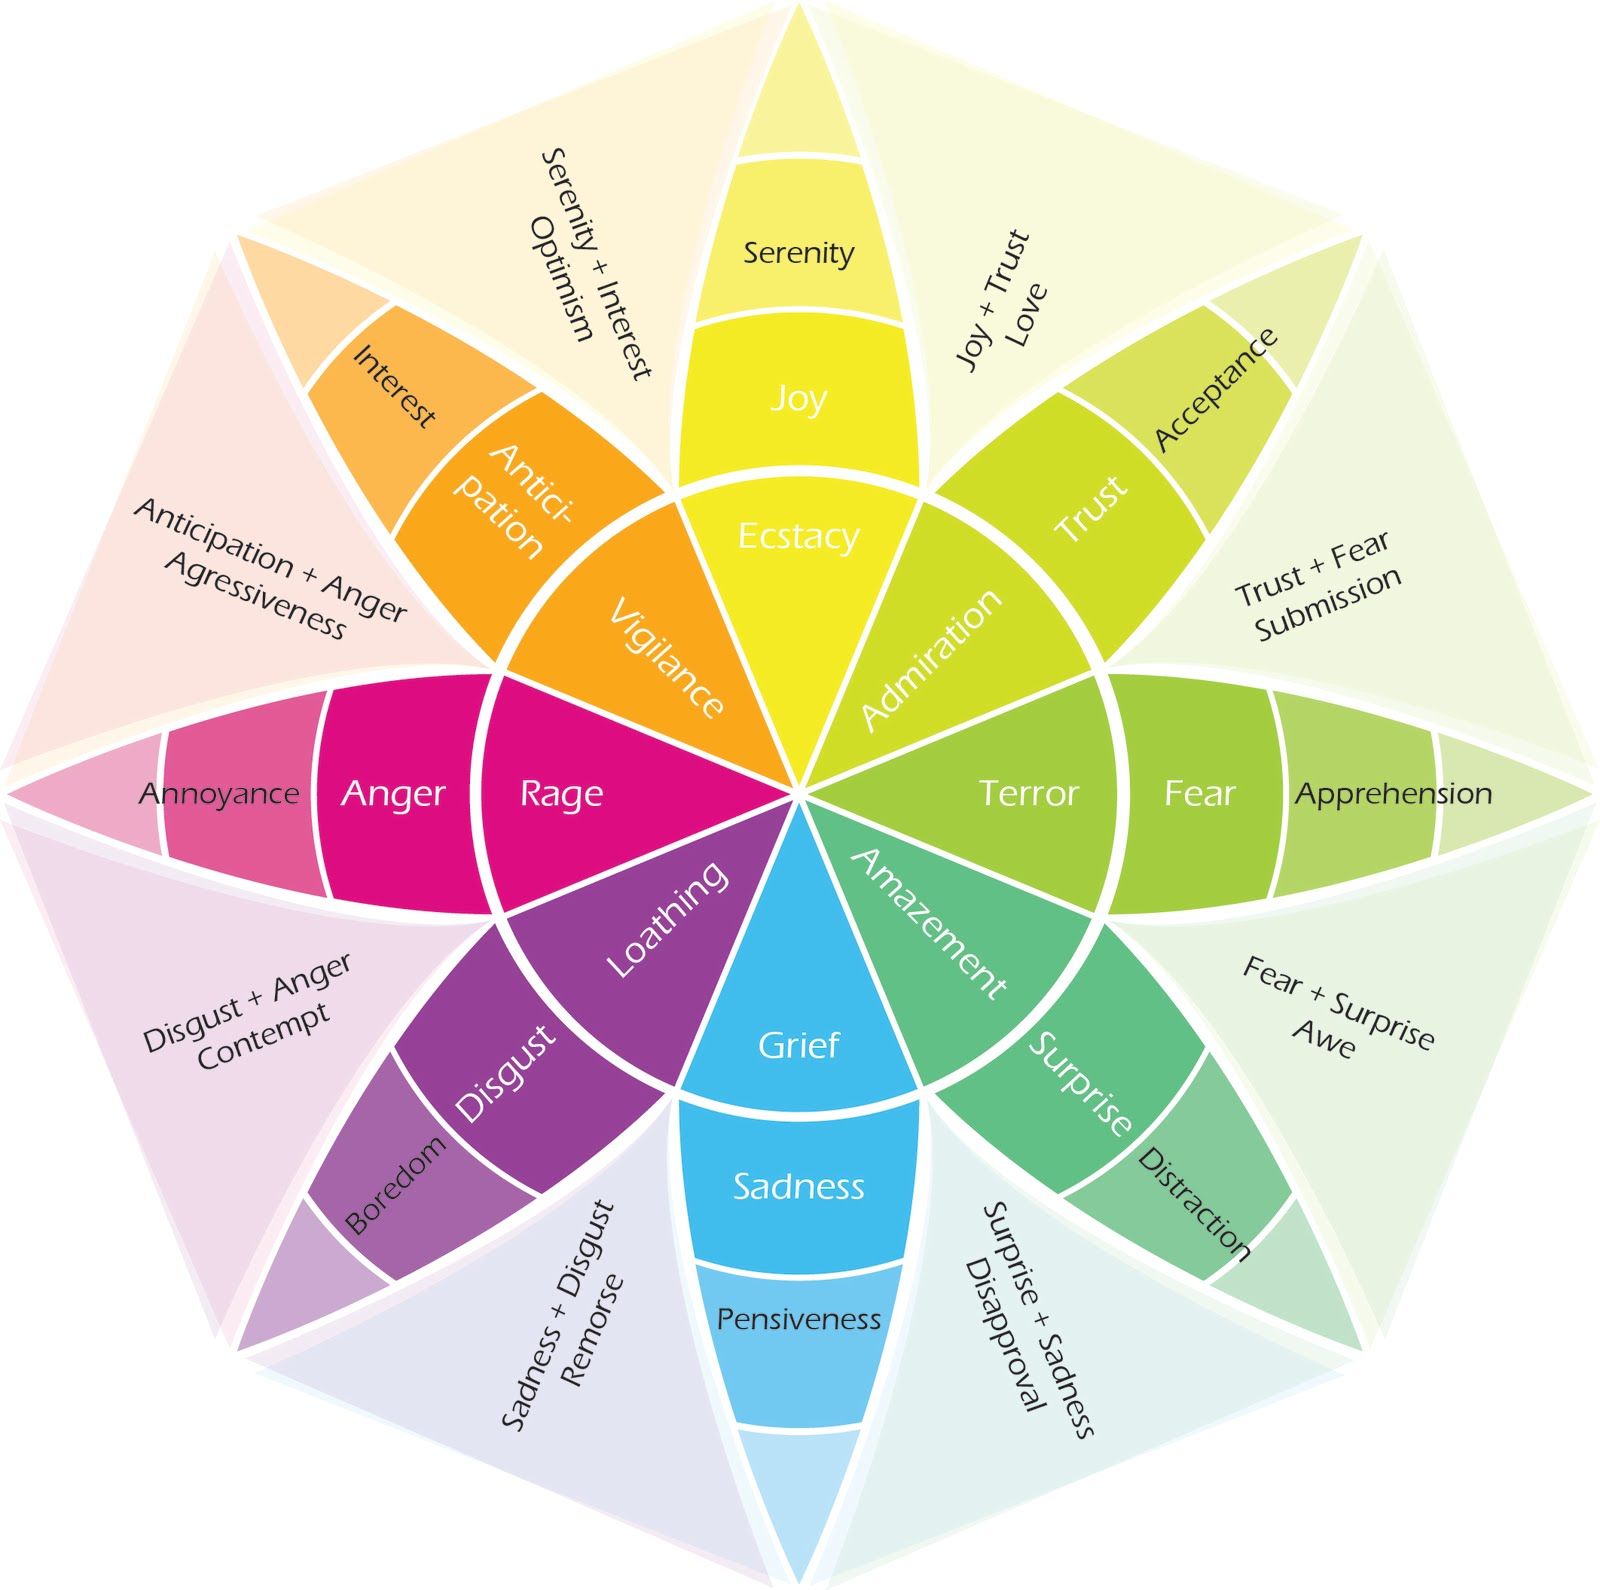
\includegraphics[width=\textwidth]{figures/plutchik_emotion_solid.jpg}}}$
        \label{fig_2d}
    \end{subfigure} \hspace{0.05\textwidth} %
    \begin{subfigure}[c]{0.25\textwidth}
        \centering

        $\vcenter{\hbox{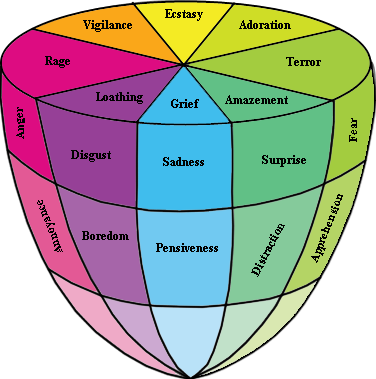
\includegraphics[width=\textwidth]{figures/plutchik_solid.png}}}$
        \label{fig_3d}
    \end{subfigure}
    \caption{A flattened and 3D view of the Emotion Structure}
    \label{fig_emotionsolid}
\end{figure}

\hrule

\paragraph{Source} \cite{robert1980emotion, block1957studies,
conte1976circumplex}

\paragraph{Depends On} --

\paragraph{Ref. By} \cref{C_ComplexEmotion}, \tref{T_GetEmotionStatePAD},
\tyref{TY_EmotionKind} \\\hrule\vspace{0.5mm}\hrule

~\newline

\noindent
\begin{minipage}{\textwidth}
    \renewcommand*{\arraystretch}{1.5}
    \begin{tabular}{| p{\colAwidth}  p{\colBwidth}|}
        \hline
        \rowcolor[gray]{0.9}
        \bf C\refstepcounter{conceptnum}\theconceptnum \label{C_ComplexEmotion}
        &\bf Mixing Emotions (PES) \\\hline
    \end{tabular}
\end{minipage}

\paragraph{Description} PES states that complex emotions are mixtures of
emotion types and intensity. It uses a colour wheel analogy to describe how to
mix them, where Emotion categories are hues and intensity is saturation.

In the PES structural model (\cref{C_EmotionStruct}), the tip of the cone has
no colour saturation whereas the circular plane is fully saturated with colour,
respectively representing no intensity and full intensity.
\\\hrule

\paragraph{Source} \cite{robert1980emotion}

\paragraph{Depends On} \cref{C_EmotionStruct}

\paragraph{Ref. By} \rref{R_MixingEmotionsPES}, \rref{R_PartitionEmotions}
\\\hrule\vspace{0.5mm}\hrule

\newpage\noindent
\begin{minipage}{\textwidth}
    \renewcommand*{\arraystretch}{1.5}
    \begin{tabular}{| p{\colAwidth}  p{\colBwidth}|}
        \hline
        \rowcolor[gray]{0.9}
        \bf C\refstepcounter{conceptnum}\theconceptnum
        \label{C_ComplexEmotions-CTE}
        &\bf ``Complex'' Emotions (CTE) \\\hline
    \end{tabular}
\end{minipage}

\paragraph{Description} CTE proposes that ``complex'' emotions are elaborations
of the emotion ``modes'' (\cref{C_Appraisal-CTE}), where the system ascribes
additional propositional meanings to it. For example, \textit{Disgust} is
typically called \textit{Contempt}, \textit{Disdain}, or \textit{Hatred} when
felt towards people instead of food, toxins, and/or
contamination~\citep[p.~60]{oatley1992best}. This also means that ``[e]motions
are in part socially constructed, but they are constructed around a biological
basis.''~\citep[p.~119]{oatley1992best}

This often requires a ``model of the self'' to draw meaning from, developed via
individual differences and culture. This model is also tied to the individual's
relationships with others (\cref{C_Relation-CTE}). \\\hrule

\paragraph{Source} \cite{oatley1987towards, oatley1992best}

\paragraph{Depends On} \cref{C_Appraisal-CTE}, \cref{C_Relation-CTE}

\paragraph{Ref. By} \tref{T_CalculateEmotionAcceptance},
\rref{R_MixingEmotionsCTE} \\\hrule\vspace{0.5mm}\hrule

~\newline

\noindent
\begin{minipage}{\textwidth}
    \renewcommand*{\arraystretch}{1.5}
    \begin{tabular}{| p{\colAwidth}  p{\colBwidth}|}
        \hline
        \rowcolor[gray]{0.9}
        \bf C\refstepcounter{conceptnum}\theconceptnum
        \label{C_PAD}
        &\bf PAD Space \\\hline
    \end{tabular}
\end{minipage}

\paragraph{Description} Based on studies in a variety of related fields with
the goal of quantifying different types of affective phenomena (e.g. emotion,
core affect, mood, personality), PAD describes describes a small set of nearly
orthogonal dimensions for analysing emotional states and behaviours, while as
relating them to other affect types and experiences. Points in this space can
represent different affective phenomena. The dimensions are present in all
affective reactions that are operative in any situation:
\begin{itemize}
    \item \textit{Pleasure} measures the positive-negative aspects of the
    emotion state (related to \textit{valence}),

    \item \textit{Arousal} is how alert and active the individual is in that
    state, and

    \item \textit{Dominance} is how much control the individual feels they have
    in that state.
\end{itemize}

The range of each dimension is $-1$ to $1$ representing mean ratings for
emotion terms. Means are based on ratings from $16$ to $31$ subjects,
transformed to the $-1$ to $1$ scale. Statistical significance---measured from
a mean of $0$ with $(p > 0.01)$---and standard deviations differ between
ratings.

Three dimensions are optimal for general characterizations and measurements of
emotional states, as two dimensions cannot distinguish between clusters of
affect and additional dimensions added little value to evaluations\\\hrule

\paragraph{Source} \cite{mehrabian1980basic, mehrabian1996pleasure}

\paragraph{Depends On} --

\paragraph{Ref. By} \tref{T_GetEmotionStatePAD}, \tyref{TY_PAD}
\\\hrule\vspace{0.5mm}\hrule

~\newpage

\noindent
\begin{minipage}{\textwidth}
    \renewcommand*{\arraystretch}{1.5}
    \begin{tabular}{| p{\colAwidth}  p{\colBwidth}|}
        \hline
        \rowcolor[gray]{0.9}
        \bf C\refstepcounter{conceptnum}\theconceptnum \label{C_Appraisal-CTE}
        &\bf Emotion Modes (CTE) \\\hline
    \end{tabular}
\end{minipage}

\paragraph{Description} CTE hypothesizes that a system can change its emotion
``mode'' (i.e. type) at plan junctures, identifiable by changes in the likely
success of a plan (\cref{C_Plans}). These junctures are assumed to be
distinctive and recurring. The system enters a ``mode'' based on the current
plan state and if/how goals (\cref{C_Goals}) are impacted, and form the basis
for other emotion ``types'' (see \cref{C_ComplexEmotions-CTE}).

\begin{table}[H]
    \centering
    \label{tab:cte_pattern}
    \renewcommand{\arraystretch}{1.2}
    \begin{tabular}{lll}
        \toprule
        \textbf{Emotion} & \textbf{Juncture of Current Plan} & \textbf{Next
        State} \\ \midrule

        \rowcolor[gray]{0.9}\textit{Happiness} & Sub-goals being achieved &
        Continue, modifying if needed \\

        \textit{Sadness} & Failure of a major plan or loss of an active goal &
        Do nothing/Search for a new plan \\

        \rowcolor[gray]{0.9}\textit{Anxiety} & Self-preservation goal
        threatened & Stop, Attend to Environment/Escape \\

        \textit{Anger} & Active plan frustrated & Try harder/Aggress \\

        \rowcolor[gray]{0.9}\textit{Disgust} & Gustatory goal violated & Reject
        substance/Withdraw \\

        \bottomrule
    \end{tabular}
\end{table}

CTE proposes that the emotion ``modes'' inhibit each other, and there might
also be conflicts that prevent the system from settling into a ``mode''. Being
in an emotion ``mode'' is a necessary---but not sufficient---condition to
experience emotion. A true emotion also requires the assignment of meaning to
the ``mode'' and the scheduling of voluntary actions. \\\hrule

\paragraph{Source} \cite{oatley1987towards, oatley1992best}

\paragraph{Depends On} \cref{C_Goals}, \cref{C_Plans}

\paragraph{Ref. By} \cref{C_ComplexEmotions-CTE}, \cref{C_EmOther},
\cref{C_EmIntensity-CTE}, \tref{T_CalculateEmotionGP}
\\\hrule\vspace{0.5mm}\hrule

~\newline

\noindent
\begin{minipage}{\textwidth}
    \renewcommand*{\arraystretch}{1.5}
    \begin{tabular}{| p{\colAwidth}  p{\colBwidth}|}
        \hline
        \rowcolor[gray]{0.9}
        \bf  C\refstepcounter{conceptnum}\theconceptnum \label{C_EmOther} & \bf
        ``Other Emotions''\\ \hline
    \end{tabular}
\end{minipage}

\paragraph{Description} Researchers continue to debate if \textit{Surprise} and
\textit{Interest} are ``emotions''. CTE is unsure of their status, but proposes
that:
\begin{itemize}
    \item \textit{Surprise} ``...is elicited by a sudden unexpected
    event...''~\citep[p.~33]{oatley1987towards}. This seems to align with the
    ``stopping'' behaviour tendencies that PES associates with
    \textit{Surprise}. Sudden, unexpected events cause \textit{Surprise}, and
    could represent an interruption and abrupt transition to another emotion
    ``mode'' (\cref{C_Appraisal-CTE})

    \item \textit{Interest} ``...implies sustained attention to certain external
    events''~\citep[p.~33]{oatley1987towards} (\cref{C_Attention}). This seems
    to align with the ``starting'' behaviour tendencies that PES associates
    with \textit{Interest}
\end{itemize}

Both descriptions imply that \textit{Surprise} and \textit{Interest} can
coexist with, or are part of, other emotion ``modes''.\\\hrule

\paragraph{Source} \cite{oatley1987towards, oatley1992best},
\cite{plutchik1984emotions}

\paragraph{Depends On} \cref{C_Appraisal-CTE}, \cref{C_Attention}

\paragraph{Ref. By} \tref{T_CalculateEmotionInterest},
\tref{T_CalculateEmotionSurprise}
\\\hrule\vspace{0.5mm}\hrule

~\newline

\noindent
\begin{minipage}{\textwidth}
    \renewcommand*{\arraystretch}{1.5}
    \begin{tabular}{| p{\colAwidth}  p{\colBwidth}|}
        \hline
        \rowcolor[gray]{0.9}
        \bf C\refstepcounter{conceptnum}\theconceptnum
        \label{C_EmIntensity-CTE}
        &\bf Emotion Intensity (CTE) \\\hline
    \end{tabular}
\end{minipage}

\paragraph{Description} Overall, emotion intensity is a relatively understudied
topic. CTE proposes that the intensity of an emotion (\cref{C_Emotion})
corresponds to how entrained the system is in a ``mode''
(\cref{C_Appraisal-CTE}) and to what degree it is ``locked into'' it. There
appear to be four determinant categories of emotion intensity evaluation:
\begin{itemize}
    \item How much the entity ``values'' affected internal conditions (e.g.
    goals),
    \item The ``seriousness'' or ``value'' of the event that affected those
    internal conditions,
    \item Contextual considerations of elements such as coping, support, and
    unexpectedness, and
    \item The entity's personality attributes that affect factors such as
    emotion response thresholds and dispositions towards different emotions.
\end{itemize}\hrule

\paragraph{Source} \cite{frijda1992complexity, oatley1987towards,
oatley1992best}

\paragraph{Depends On} \cref{C_Emotion}, \cref{C_Appraisal-CTE}

\paragraph{Ref. By} \tref{T_CalculateEmotionIntensity}
\\\hrule\vspace{0.5mm}\hrule

~\newline

\noindent
\begin{minipage}{\textwidth}
    \renewcommand*{\arraystretch}{1.5}
    \begin{tabular}{| p{\colAwidth}  p{\colBwidth}|}
        \hline
        \rowcolor[gray]{0.9}
        \bf  C\refstepcounter{conceptnum}\theconceptnum \label{C_EmDecay} & \bf
        Emotion Decay\\ \hline
    \end{tabular}
\end{minipage}

\paragraph{Description} Emotions (\cref{C_Emotion}) do not last
indefinitely---they dissipate after a time, implying the presence of an emotion
decay mechanism. This requires a specification of baseline values for each
emotion and as well as one or more decay functions. \\\hrule

\paragraph{Source} \cite{broekens2021emotion}

\paragraph{Depends On} \cref{C_Emotion}

\paragraph{Ref. By} \tref{T_DecayEmotionState} \\\hrule\vspace{0.5mm}\hrule

~\newline

\clearpage\noindent
\begin{minipage}{\textwidth}
    \renewcommand*{\arraystretch}{1.5}
    \begin{tabular}{| p{\colAwidth}  p{\colBwidth}|}
        \hline
        \rowcolor[gray]{0.9}
        \bf C\refstepcounter{conceptnum}\theconceptnum \label{C_Goals} & \bf
        Goals \\\hline
    \end{tabular}
\end{minipage}

\paragraph{Description} Goals compel systems to act in ways that achieve a
desired objective. They are essential for emotion processing, identifying what
elements of the current world state are relevant to an individual rather than
relying on properties of the environment alone. Entities use goals to know when
events impact them and by how much. Goals are also connected to emotions,
partially motivating emotion-driven behaviours.

PES describes goals as being in service to global adaptational problems,
whereas CTE view them as symbolic representations of possible environmental
states that a system wants to achieve. \\\hrule

\paragraph{Source} \cite{oxfordGoals}, \citet[p.~223]{broekens2016emotional},
\cite{robert1980emotion, oatley1987towards}, \citet[p.~208]{ortony2002making}

\paragraph{Depends On} --

\paragraph{Ref. By} \cref{C_Emotion}, \cref{C_Appraisal-CTE}, \cref{C_Plans},
\tref{T_CalculateEmotionGP}, \tyref{TY_Goal} \\\hrule\vspace{0.5mm}\hrule

~\newline

\noindent
\begin{minipage}{\textwidth}
    \renewcommand*{\arraystretch}{1.5}
    \begin{tabular}{| p{\colAwidth}  p{\colBwidth}|}
        \hline
        \rowcolor[gray]{0.9}
        \bf C\refstepcounter{conceptnum}\theconceptnum \label{C_Plans} & \bf
        Plans (CTE) \\\hline
    \end{tabular}
\end{minipage}

\paragraph{Description} CTE describes plans as sequences of transformations
between symbolic representations of possible environmental states, linking the
current state to a goal (\cref{C_Goals}). To ``make'' a plan is to create a
sequence of transformations, and to ``execute'' the plan is to enact the
sequence in the world.

A system forms plans with imperfect and incomplete knowledge of the
environment, and often only looks one or two steps ahead. \\\hrule

\paragraph{Source} \cite{oatley1987towards}

\paragraph{Depends On} \cref{C_Goals}

\paragraph{Ref. By} \cref{C_Appraisal-CTE}, \tref{T_CalculateEmotionGP},
\tyref{TY_Plan} \\\hrule\vspace{0.5mm}\hrule

~\newline

\noindent
\begin{minipage}{\textwidth}
    \renewcommand*{\arraystretch}{1.5}
    \begin{tabular}{| p{\colAwidth}  p{\colBwidth}|}
        \hline
        \rowcolor[gray]{0.9}
        \bf C\refstepcounter{conceptnum}\theconceptnum \label{C_Relation-CTE} &
        \bf Social Relationship \\\hline
    \end{tabular}
\end{minipage}

\paragraph{Description} CTE states that many emotions are social, occurring in
the course of one's relationships with others. This allows them to construct
mutual plans to coordinate the actions of multiple actors, which also requires
each actor to have a ``model of the self''.

The emotion of \textit{Acceptance} (i.e. \textit{Trust})---an elementary
component of social life---in PES also implies the existence of relationships
with others. ``Affective trust'' builds on past experiences with, feelings of
security, confidence, and satisfaction towards, and the perceived level of
selfless concern demonstrated by a partner regardless of what the future holds.
The biological basis of affective trust might lie in social attachment and
affiliation due to the role of oxytocin.

A social relationship is a representation of the history shared between the
individual and another person, entity, or thing. They can be established
implicitly based on precedents and customs (i.e. culture). \\\hrule

\paragraph{Source} \cite{oatley1987towards, oxfordTrust, rempel1985trust}

\paragraph{Depends On} --

\paragraph{Ref. By} \cref{C_ComplexEmotions-CTE},
\tref{T_CalculateEmotionAcceptance}, \tyref{TY_Relation-CTE}
\\\hrule\vspace{0.5mm}\hrule

~\newline

\noindent
\begin{minipage}{\textwidth}
    \renewcommand*{\arraystretch}{1.5}
    \begin{tabular}{| p{\colAwidth}  p{\colBwidth}|}
        \hline
        \rowcolor[gray]{0.9}
        \bf C\refstepcounter{conceptnum}\theconceptnum \label{C_Attention} &
        \bf Attention \\\hline
    \end{tabular}
\end{minipage}

\paragraph{Description} Attention is a set of mechanisms that allow a
limited-capacity system to select salient or goal-relevant information. These
mechanisms might work in parallel. Behavioural effects of attention vary
between systems, partially due to personality. \\\hrule

\paragraph{Source} \cite{oxfordAttention}

\paragraph{Depends On} --

\paragraph{Ref. By} \cref{C_EmOther}, \tyref{TY_Attention}
\\\hrule\vspace{0.5mm}\hrule

\newpage

\subsubsection{Theoretical Models}\label{sec_theoretical}

These models refine the Conceptual Models (Section~\ref{sec_conceptual}) using
natural language to improve their precision. This is a necessary step for
reducing ambiguity by explicitly stating how the primary sources are understood
and showing how they relate to the mathematically-defined Data Types
(Section~\ref{sec_typedefs}) and Instance Models (Section~\ref{sec_instance})
using Assumptions (Section~\ref{sec_assumptions}).

~\newline\noindent
\begin{minipage}{\textwidth}
    \renewcommand*{\arraystretch}{1.5}
    \begin{tabular}{| p{\colAwidth}  p{\colBwidth}|}
        \hline
        \rowcolor[gray]{0.9}
        \bf T\refstepcounter{theorynum}\thetheorynum
        \label{T_CalculateEmotionGP} &
        \bf Evaluate Emotion Kind from Goals and Plans \\
        \hline
    \end{tabular}
\end{minipage}

\paragraph{Description} The emotion kinds (``modes'') that CTE defines
(\cref{C_Appraisal-CTE})---\textit{Happiness}, \textit{Sadness}, \textit{Fear},
\textit{Anger}, \textit{Disgust}---in terms of goals (\cref{C_Goals}) and plans
(\cref{C_Plans}) can be re-conceptualized as follows:
\begin{itemize}
    \item \textit{Joy} (\textit{Happiness}) occurs when an action moves an
    entity closer to achieving a goal, assuming that each such action is a goal
    itself (i.e. a ``sub-goal'' of the goal, \aref{A_Subgoal})

    \item \textit{Sadness} occurs when an entity has a plan where a next step
    is impossible to achieve (i.e. ``failure of a plan''), or a goal becomes
    impossible to achieve (i.e. ``loss of a goal'')

    \item \textit{Fear} (\textit{Anxiety}) occurs when there is a threat to
    self-preservation (i.e. ``self-preservation goal threatened''), which
    requires a prediction about a future world state based on the current world
    state and an action that could change it

    \item \textit{Anger} occurs when an entity has a plan where the next step
    cannot be reached after an intentional action to achieve it, but there are
    one or more other actions that can (i.e. the plan is ``frustrated'' because
    it is still feasible, but it had to change to remain so)

    \item \textit{Disgust} occurs when an entity has been ``contaminated'' or
    encounters ``contaminated'' substances that it wants to avoid (i.e.
    ``gustatory goal violated'')
\end{itemize}

It is assumed that a single goal can trigger more than one emotion
(\aref{A_Goal2Emotion}) and they all contribute to a single emotion state
(\aref{A_OneState}).

Emotion intensity is evaluated separately (\aref{A_EmotionTypeIntensity}, see
\tref{T_CalculateEmotionIntensity}). The emotions \textit{Surprise},
\textit{Interest}, and \textit{Acceptance} are evaluated differently because
they are not part of CTE's primary emotions (\aref{A_AppraisalProcess}, see
\tref{T_CalculateEmotionSurprise}, \tref{T_CalculateEmotionInterest}, and
\tref{T_CalculateEmotionAcceptance} respectively). \\\hrule

\paragraph{Sources} --

\paragraph{Depends On} \aref{A_Subgoal}, \aref{A_Goal2Emotion},
\aref{A_OneState}, \aref{A_EmotionTypeIntensity},
\aref{A_AppraisalProcess}, \cref{C_Appraisal-CTE}, \cref{C_Goals},
\cref{C_Plans}

\paragraph{Ref. By} \iref{IM_CalculateEmotionGP} \\\hrule\vspace{0.5mm}\hrule

~\newpage\noindent
\begin{minipage}{\textwidth}
    \renewcommand*{\arraystretch}{1.5}
    \begin{tabular}{| p{\colAwidth}  p{\colBwidth}|}
        \hline
        \rowcolor[gray]{0.9}
        \bf T\refstepcounter{theorynum}\thetheorynum
        \label{T_CalculateEmotionIntensity} &
        \bf Evaluate Emotion Intensity \\
        \hline
    \end{tabular}
\end{minipage}

\paragraph{Description} Emotion intensity (\cref{C_EmIntensity-CTE}) is
proportional to the force causing an emotion state (``entrained'') and how
fixed or non-adjustable that force is (``locked in''). This could be related to
the degree that something impacts a goal (\aref{A_Goal2Intensity})---either a
stand-alone goal or as part of a plan (i.e. a ``sub-goal'')---such that an
entity would want to maintain the momentum caused by an emotion ``mode'' as
long as that goal is affected. \\\hrule

\paragraph{Sources} --

\paragraph{Depends On} \aref{A_Goal2Intensity}, \cref{C_EmIntensity-CTE}

\paragraph{Ref. By} \tyref{TY_EmotionIntensity},
\iref{IM_CalculateEmotionIntensity} \\\hrule\vspace{0.5mm}\hrule

~\newline

\noindent
\begin{minipage}{\textwidth}
    \renewcommand*{\arraystretch}{1.5}
    \begin{tabular}{| p{\colAwidth}  p{\colBwidth}|}
        \hline
        \rowcolor[gray]{0.9}
        \bf T\refstepcounter{theorynum}\thetheorynum
        \label{T_CalculateEmotionSurprise} &
        \bf Evaluate \textit{Surprise} Emotion and Intensity \\
        \hline
    \end{tabular}
\end{minipage}

\paragraph{Description} An ``interruption and abrupt transition'' to a
different emotion state elicits \textit{Surprise} (\cref{C_EmOther}). This
suggests that it occurs when there is a large, rapid change in emotion
intensity (\aref{A_Surprise}), and/or there the emotion state recently changed
and it is changing again (``sudden, unexpected event'', \aref{A_Surprise2}).

For intensity, this implies that it is inversely proportional to time such that
less time it takes for the emotion intensity change to occur and/or between the
recently changed emotion state and the current change to a ``new'' emotion
state creates a higher intensity response. Intensity rapidly decreases as time
elapses. \\\hrule

\paragraph{Sources} --

\paragraph{Depends On} \aref{A_Surprise}, \aref{A_Surprise2}, \cref{C_EmOther}

\paragraph{Ref. By} \tyref{TY_EmotionIntensity},
\iref{IM_CalculateEmotionSurpriseElicit}, \iref{IM_CalculateEmotionSurprise}
\\\hrule\vspace{0.5mm}\hrule

~\newline

\noindent
\begin{minipage}{\textwidth}
    \renewcommand*{\arraystretch}{1.5}
    \begin{tabular}{| p{\colAwidth}  p{\colBwidth}|}
        \hline
        \rowcolor[gray]{0.9}
        \bf T\refstepcounter{theorynum}\thetheorynum
        \label{T_CalculateEmotionInterest} &
        \bf Evaluate \textit{Interest} Emotion and Intensity \\
        \hline
    \end{tabular}
\end{minipage}

\paragraph{Description} ``Sustained attention to certain external events''
elicits \textit{Interest} (\cref{C_EmOther}), implying that it occurs when an
entity is focused on the same thing (e.g. task, another entity) for an extended
period of time (\aref{A_Interest}). This suggests that there is a ``baseline''
amount of attention/time paid to something before it triggers
\textit{Interest}, which can differ between foci.

For intensity, this implies that it is proportional to the amount of time spent
focused on the same thing and relative to the ``baseline'' time spent. \\\hrule

\paragraph{Sources} --

\paragraph{Depends On} \aref{A_Interest}, \cref{C_EmOther}

\paragraph{Ref. By} \tyref{TY_EmotionIntensity},
\iref{IM_CalculateEmotionInterestElicit}, \iref{IM_CalculateEmotionInterest}
\\\hrule\vspace{0.5mm}\hrule

~\newline

\noindent
\begin{minipage}{\textwidth}
    \renewcommand*{\arraystretch}{1.5}
    \begin{tabular}{| p{\colAwidth}  p{\colBwidth}|}
        \hline
        \rowcolor[gray]{0.9}
        \bf T\refstepcounter{theorynum}\thetheorynum
        \label{T_CalculateEmotionAcceptance} &
        \bf Evaluate \textit{Acceptance} Emotion and Intensity \\
        \hline
    \end{tabular}
\end{minipage}

\paragraph{Description} Taking \textit{Acceptance} as a ``complex'' emotion
(\cref{C_ComplexEmotions-CTE}), it can be defined as \textit{Joy}
(\textit{Happiness}) elaborated with information about social relationships
(\cref{C_Relation-CTE}) such that an entity experiences \textit{Acceptance}
when it attributes a state of \textit{Joy} to another entity that they have an
established relationship with (\aref{A_Acceptance}). An entity might also
establish a relationship with another entity that is attributed with causing
the state, which would also elicit \textit{Acceptance}.

For intensity, this implies that it is proportional to the intensity of
\textit{Joy} and the strength of the relationship with the entity that the
state is attributed to. \\\hrule

\paragraph{Sources} \citet[p.~178--179]{oatley1992best}

\paragraph{Depends On} \aref{A_Acceptance}, \cref{C_ComplexEmotions-CTE},
\cref{C_Relation-CTE}

\paragraph{Ref. By} \tyref{TY_EmotionIntensity},
\iref{IM_CalculateEmotionAcceptanceElicit},
\iref{IM_CalculateEmotionAcceptance} \\\hrule\vspace{0.5mm}\hrule

~\newline

\noindent
\begin{minipage}{\textwidth}
    \renewcommand*{\arraystretch}{1.5}
    \begin{tabular}{| p{\colAwidth}  p{\colBwidth}|}
        \hline
        \rowcolor[gray]{0.9}
        \bf T\refstepcounter{theorynum}\thetheorynum
        \label{T_DecayEmotionState} &
        \bf Decaying Emotion State \\
        \hline
    \end{tabular}
\end{minipage}

\paragraph{Description} Emotion decay (\cref{C_EmDecay}) is a function of time
such that the emotion state returns to its ``equilibrium'' intensities as time
progresses. It is assumed that:
\begin{itemize}
    \item The speed that intensities return to ``equilibrium'' are assumed to
    be functions of distance such that larger differences between an intensity
    and its ``equilibrium'' cause larger changes in intensity
    (\aref{A_DecaySpeed})

    \item Each emotion kind has its own ``equilibrium'' value
    (\aref{A_Equilibrium}) and can decay at different rates (\aref{A_DecayRate})

    \item Decay rates and equilibrium values can differ between entities
    (\aref{A_DecayUnique})
\end{itemize}
\hrule

\paragraph{Sources} --

\paragraph{Depends On} \aref{A_DecaySpeed}, \aref{A_Equilibrium},
\aref{A_DecayRate}, \aref{A_DecayUnique}, \cref{C_EmDecay}

\paragraph{Ref. By} \tyref{TY_EmotionDecay}, \tyref{TY_EmotionDecayState},
\iref{IM_DecayEmotionState} \\\hrule\vspace{0.5mm}\hrule

~\clearpage

\noindent
\begin{minipage}{\textwidth}
    \renewcommand*{\arraystretch}{1.5}
    \begin{tabular}{| p{\colAwidth}  p{\colBwidth}|}
        \hline
        \rowcolor[gray]{0.9}
        \bf T\refstepcounter{theorynum}\thetheorynum
        \label{T_GetEmotionStatePAD} &
        \bf Getting an Emotion State as a PAD Point \\
        \hline
    \end{tabular}
\end{minipage}

\paragraph{Description} Assuming that an entity can only occupy one point in
PAD Space at any given time (\aref{A_OnePADPoint}), the intensities for each
discrete emotion in an emotion state must be combined into a single value for
each dimension in the space. This requires reference points for each emotion
type in PES because it defines the emotion state structure
(\cref{C_EmotionStruct}) that emotion intensities are mapped to.

In both theories, laypeople evaluated emotion terms for their contents. In both
experiments, the laypeople were likely from the same age group (university
undergraduates, college and graduate students), likely from the United States
(in the case of PAD, Californian), and likely to have participated in the
experiments around the same time given the publishing year of the work (1980).
Therefore, it is reasonable to assume that the meaning of the terms in PES and
PAD Space would be judged to be identical or nearly identical to each other by
the same laypeople (\aref{A_EmotionTerms}).

The circumplex representing the relative similarity of emotion term
meanings~\citep[p.~170]{robert1980emotion} was divided into ranges,
representing what language laypeople typical describe PES emotion kinds with.
Gaps between areas are small (0.3\textdegree{} at least, 7.3\textdegree{} at
most), so they are ignored. The list of 145 emotion terms from PES and 151 from
PAD~\citep[p.~42--45]{mehrabian1980basic} were compared for common terms, which
were listed by PES emotion kind. An emotion term was selected from each list
based on its similarity to the emotion kind label. There was no such term for
\textit{Acceptance}, so \progname{} uses the term closest to the mean range on
the circumplex (i.e. ``Affectionate''). Where possible, emotion terms that had
statistical significance ($p < 0.01$) for all dimensions define reference
points (e.g. \textit{Astonished} is statistically significant on all three
dimensions, whereas \textit{Surprised} is only significant for two). All terms
achieved significance for \textit{pleasure} and \textit{arousal}.
\textit{Interested} and \textit{Disgust} are not statistically significant for
\textit{dominance}.

An emotion term's \textit{pleasure}, \textit{arousal}, and \textit{dominance}
mean values (\cref{C_PAD}) form a reference point. Number of ratings and
standard deviation do not affect reference points (\aref{A_PADStats}).

\begin{table}[H]
    \centering
    \renewcommand{\arraystretch}{1.2}
    \begin{tabular}{ccccc}
        \toprule
        \multicolumn{2}{c}{\textbf{PES}} &  &  & \\
        $k \in \emotionkindstype$ & Range on Circumplex (\textdegree) & Term  &
        Circumplex Location (\textdegree) & PAD Ref.~\# \\
        \midrule

        \rowcolor[gray]{0.9}\textit{Fear} & $[65.0, 86.0]$ & Terrified & 75.5 &
        102 \\

        \textit{Anger} & $[200.6, 249.0]$ & Angry & 212.0 & 82 \\

        \rowcolor[gray]{0.9}\textit{Sadness} & $[88.3, 138.0]$ & Sad & 108.5 &
        151 \\

        \textit{Joy} & $[323.4, 338.3]$ & Joyful & 323.4 & 20 \\

        \rowcolor[gray]{0.9}\textit{Interest} & $[249.7, 322.4]$ & Interested &
        315.7 & 8 \\

        \textit{Surprise} & $[138.3, 156.7]$ & Astonished & 148.0 & 74 \\

        \rowcolor[gray]{0.9}\textit{Disgust} & $[160.3, 193.7]$ & Disgusted &
        161.3 & 75 \\

        \textit{Acceptance} & $[340.7, 57.7]$ & Affectionate & 52.3 & 34 \\

        \bottomrule
    \end{tabular}
\end{table}

\hrule

\paragraph{Sources} \citet[p.~40, 42--45]{mehrabian1980basic},
\citet[p.~159, 170]{robert1980emotion}, \cite{conte1976circumplex}

\paragraph{Depends On} \aref{A_OnePADPoint}, \aref{A_EmotionTerms},
\aref{A_PADStats}, \cref{C_EmotionStruct}, \cref{C_PAD}

\paragraph{Ref. By} \iref{IM_GetEmotionStatePAD} \\\hrule\vspace{0.5mm}\hrule

\newpage

\subsubsection{General Definitions}\label{sec_gendef}

No additional information is required to build the data definitions.

\subsubsection{Data Definitions}\label{sec_datadef}

No data definitions are needed.

\newpage

\subsubsection{Data Types}\label{sec_typedefs}
This section defines types for realizing \progname{}'s Instance Models
(Section~\ref{sec_instance}). Data types also allow for type checking to verify
and enforce constraints (Section~\ref{sec_DataConstraints}), and defining model
interfaces.

Data types \tyref{TY_Time}, \tyref{TY_WorldState}, \tyref{TY_WorldStateChange},
\tyref{TY_DistanceBetweenWorldStates},
\tyref{TY_DistanceBetweenWorldStatesChange}, \tyref{TY_Goal}, \tyref{TY_Plan},
\tyref{TY_Attention}, and \tyref{TY_Relation-CTE} are APIs for users to
implement for their specific needs.
\begin{itemize}
    \item \tyref{TY_Time}, \tyref{TY_WorldState}, \tyref{TY_WorldStateChange},
    \tyref{TY_DistanceBetweenWorldStates},
    \tyref{TY_DistanceBetweenWorldStatesChange}, and \tyref{TY_Goal} are
    mandatory

    \item \tyref{TY_Plan} is optional, but necessary for \textit{Anger}

    \item \tyref{TY_Attention} is optional, but necessary for \textit{Interest}

    \item \tyref{TY_Relation-CTE} is optional, but necessary for
    \textit{Acceptance}
\end{itemize}

~\newline\noindent
\begin{minipage}{\textwidth}
    \renewcommand*{\arraystretch}{1.5}
    \begin{tabular}{| p{\colAwidth}  p{\colBwidth}|}
        \hline
        \rowcolor[gray]{0.9}
        \bf TY\refstepcounter{typenum}\thetypenum
        \label{TY_Time} & \bf Type of Time and Delta Time \\
        \hline
    \end{tabular}

    \renewcommand*{\arraystretch}{1.5}
    \begin{tabular}{ p{\colAwidth}  p{\colBwidth}}
        \bf Symbol & $\timetype, \deltatimetype$ \\

        \bf Type & -- \\\hline
    \end{tabular}
\end{minipage}

\paragraph{Description} Time is an abstract type that is linearly ordered. A
Delta Time is the difference between two Time values. \\\hrule

\paragraph{Sources} --

\paragraph{Depends On} --

\paragraph{Ref. By} \tyref{TY_Emotion}, \tyref{TY_Attention},
\iref{IM_CalculateEmotionSurpriseElicit}, \iref{IM_CalculateEmotionSurprise},
\iref{IM_DecayEmotionState}, \iref{IM_UpdateEmotion},
\iref{IM_GetEmotionState}, \iref{IM_DecayEmotion}, \rref{R_TimeType}
\\\hrule\vspace{0.5mm}\hrule

~\newline

\noindent
\begin{minipage}{\textwidth}
    \renewcommand*{\arraystretch}{1.5}
    \begin{tabular}{| p{\colAwidth}  p{\colBwidth}|}
        \hline
        \rowcolor[gray]{0.9}
        \bf TY\refstepcounter{typenum}\thetypenum
        \label{TY_EmotionIntensity} & \bf Type of Emotion Intensity \\
        \hline
    \end{tabular}

    \renewcommand*{\arraystretch}{1.5}
    \begin{tabular}{ p{\colAwidth}  p{\colBwidth}}
        \bf Symbol & $\emotionintensitytype$ \\

        \bf Type & $ \mathbb{R}_{\geq0} $
        \\\hline
    \end{tabular}
\end{minipage}

\paragraph{Description} Emotion intensity (\tref{T_CalculateEmotionIntensity},
\tref{T_CalculateEmotionSurprise}, \tref{T_CalculateEmotionInterest},
\tref{T_CalculateEmotionAcceptance}) is a real, non-negative value
(\aref{A_PositiveIntensity}). \\\hrule

\paragraph{Sources} --

\paragraph{Depends On} \aref{A_PositiveIntensity},
\tref{T_CalculateEmotionIntensity}, \tref{T_CalculateEmotionSurprise},
\tref{T_CalculateEmotionInterest}, \tref{T_CalculateEmotionAcceptance}

\paragraph{Ref. By} \tyref{TY_DeltaIntensity}, \tyref{TY_EmotionState},
\tyref{TY_EmotionDecayState}, \iref{IM_CalculateEmotionAcceptanceElicit},
\iref{IM_DecayEmotionState}, \iref{IM_UpdateEmotionState},
\iref{IM_UpdateEmotionState2}, \rref{R_IntensityTypeUse},
\rref{R_MixingEmotionsPES}, \rref{R_PartitionEmotions}
\\\hrule\vspace{0.5mm}\hrule

~\newline

\noindent
\begin{minipage}{\textwidth}
    \renewcommand*{\arraystretch}{1.5}
    \begin{tabular}{| p{\colAwidth}  p{\colBwidth}|}
        \hline
        \rowcolor[gray]{0.9}
        \bf TY\refstepcounter{typenum}\thetypenum
        \label{TY_DeltaIntensity} & \bf Type of Emotion Intensity Change \\
        \hline
    \end{tabular}

    \renewcommand*{\arraystretch}{1.5}
    \begin{tabular}{ p{\colAwidth}  p{\colBwidth}}
        \bf Symbol & $ \responsestrength $ \\

        \bf Type & $ \mathbb{R} $ \\\hline
    \end{tabular}
\end{minipage}

\paragraph{Description} A change in emotion intensity represents the magnitude
of a difference to be applied to an emotion intensity
(\tyref{TY_EmotionIntensity}). It is a real value because:
\begin{itemize}
    \item Emotion intensity can both increase and decrease, and

    \item The magnitude of a change should not be pre-emptively constrained to
    fit the type of $\emotionintensitytype$ in case $\responsestrength$ has
    other uses
\end{itemize} \hrule

\paragraph{Sources} --

\paragraph{Depends On} \tyref{TY_EmotionIntensity}

\paragraph{Ref. By} \iref{IM_CalculateEmotionIntensity},
\iref{IM_CalculateEmotionSurprise}, \iref{IM_CalculateEmotionInterest},
\iref{IM_CalculateEmotionAcceptance}, \iref{IM_UpdateEmotionState},
\rref{R_IntensityChangeType} \\\hrule\vspace{0.5mm}\hrule

~\newline

\noindent
\begin{minipage}{\textwidth}
    \renewcommand*{\arraystretch}{1.5}
    \begin{tabular}{| p{\colAwidth}  p{\colBwidth}|}
        \hline
        \rowcolor[gray]{0.9}
        \bf TY\refstepcounter{typenum}\thetypenum
        \label{TY_EmotionDecay} & \bf Type of Emotion Intensity Decay Rate \\
        \hline
    \end{tabular}

    \renewcommand*{\arraystretch}{1.5}
    \begin{tabular}{ p{\colAwidth}  p{\colBwidth}}
        \bf Symbol & $ \emotiondecaytype $ \\

        \bf Type & $ \mathbb{R}_{>0} $ \\\hline
    \end{tabular}
\end{minipage}

\paragraph{Description} Emotion decay rate (\tref{T_DecayEmotionState}) is a
real-valued, strictly positive constant. It is equivalent to the spring
constant $k_s$ in a damped harmonic oscillator, which is always strictly
positive. \\\hrule

\paragraph{Sources}
{\small\url{https://en.wikipedia.org/wiki/Harmonic_oscillator#Damped_harmonic_oscillator}}

\paragraph{Depends On} \tref{T_DecayEmotionState}

\paragraph{Ref. By} \tyref{TY_EmotionDecayState}, \iref{IM_DecayEmotionState},
\rref{R_IntensityDecayType} \\\hrule\vspace{0.5mm}\hrule

~\newline

\noindent
\begin{minipage}{\textwidth}
    \renewcommand*{\arraystretch}{1.5}
    \begin{tabular}{| p{\colAwidth}  p{\colBwidth}|}
        \hline
        \rowcolor[gray]{0.9}
        \bf TY\refstepcounter{typenum}\thetypenum
        \label{TY_EmotionKind} & \bf Type of Emotion Kinds \\
        \hline
    \end{tabular}

    \renewcommand*{\arraystretch}{1.5}
    \begin{tabular}{ p{\colAwidth}  p{\colBwidth}}
        \bf Symbol & $\emotionkindstype$ \\

        \bf Type & $ \left< \mFear, \mAnger, \mSadness, \mJoy, \mInterest,
        \mSurprise, \mDisgust, \mTrust \right> $ \\

        \bf Invariants & $\bullet$ $\emotionkindstype$ is finite and ordered

        $\bullet$ Each element of $\emotionkindstype$ is uniquely paired with
        exactly one other element that is not itself \\
        \hline
    \end{tabular}
\end{minipage}

\paragraph{Description} Emotion kinds is an enumeration representing the
primary emotion kinds from PES (\cref{C_EmotionStruct}). ``Opposing'' emotions
as defined in PES are enforced via the invariant regarding unique pairings.
\\\hrule

\paragraph{Sources} --

\paragraph{Depends On} \cref{C_EmotionStruct}

\paragraph{Ref. By} \tyref{TY_EmotionState}, \tyref{TY_EmotionDecayState},
\iref{IM_CalculateEmotionGP}, \iref{IM_UpdateEmotionState},
\iref{IM_UpdateEmotionState2}, \iref{IM_DecayEmotion},
\iref{IM_GetEmotionStatePAD}, \rref{R_EmotionKindsType},
\rref{R_MixingEmotionsPES}, \rref{R_PartitionEmotions},
\rref{R_MixingEmotionsCTE} \\\hrule\vspace{0.5mm}\hrule

~\newline

\noindent
\begin{minipage}{\textwidth}
    \renewcommand*{\arraystretch}{1.5}
    \begin{tabular}{| p{\colAwidth}  p{\colBwidth}|}
        \hline
        \rowcolor[gray]{0.9}
        \bf TY\refstepcounter{typenum}\thetypenum
        \label{TY_EmotionState} & \bf Type of Emotion State \\
        \hline
    \end{tabular}

    \renewcommand*{\arraystretch}{1.5}
    \begin{tabular}{ p{\colAwidth}  p{\colBwidth}}
        \bf Symbol & $\emotionstatetype$ \\

        \bf Type & $ \left\{ \mathtt{intensities} : \emotionkindstype
        \rightarrow \emotionintensitytype, \mathtt{max} : \emotionkindstype
        \rightarrow \emotionintensitytype \right\}  $ \\

        \bf Invariant & $\forall k \in \emotionkindstype \Rightarrow 0 \leq
        \mathtt{intensities}(k) \leq \mathtt{max}(k) $
        (\aref{A_LimitIntensity}) \\
        \hline
    \end{tabular}
\end{minipage}

\paragraph{Description} An emotion state is a record with:
\begin{itemize}

    \item An intensity function $\mathtt{intensities}$ mapping each element in
    $\emotionkindstype$ (\tyref{TY_EmotionKind}) to an intensity value
    $\emotionintensitytype$ (\tyref{TY_EmotionIntensity})

    \item An intensity function $\mathtt{max}$ mapping each element in
    $\emotionkindstype$ (\tyref{TY_EmotionKind}) to a maximum intensity value
    $\emotionintensitytype$ (\tyref{TY_EmotionIntensity})

\end{itemize}

The invariant ensures that emotion intensity is finite
(\aref{A_LimitIntensity}). Each element in $\emotionstatetype$ is independent
(\aref{A_EmotionPairs}, \cref{C_Emotion}).\\\hrule

\paragraph{Sources} --

\paragraph{Depends On} \aref{A_LimitIntensity}, \aref{A_EmotionPairs},
\cref{C_Emotion}, \tyref{TY_EmotionIntensity}, \tyref{TY_EmotionKind}

\paragraph{Ref. By} \tyref{TY_Emotion}, \iref{IM_UpdateEmotionState2},
\iref{IM_UpdateEmotion}, \iref{IM_GetEmotionState}, \iref{IM_DecayEmotion},
\iref{IM_GetEmotionStatePAD}, \rref{R_EmotionStateType}
\\\hrule\vspace{0.5mm}\hrule

~\newline

\noindent
\begin{minipage}{\textwidth}
    \renewcommand*{\arraystretch}{1.5}
    \begin{tabular}{| p{\colAwidth}  p{\colBwidth}|}
        \hline
        \rowcolor[gray]{0.9}
        \bf TY\refstepcounter{typenum}\thetypenum
        \label{TY_EmotionDecayState} & \bf Type of Emotion State Decay \\
        \hline
    \end{tabular}

    \renewcommand*{\arraystretch}{1.5}
    \begin{tabular}{ p{\colAwidth}  p{\colBwidth}}
        \bf Symbol & $ \emotionstatedecaytype $ \\

        \bf Type & $ \left\{ \mathtt{equilibrium} : \emotionkindstype
        \rightarrow \emotionintensitytype, \mathtt{decayRates} :
        \emotionkindstype \rightarrow \emotiondecaytype \right\} $ \\

        \bf Invariants & Given an $es : \emotionstatedecaytype$,
        $\left(\mathlarger\sum_{k \in\emotionkindstype}
        es.\mathtt{equilibrium}\left(k\right)\right) > 0$
        (\aref{A_PositiveIntensity})
        \vspace*{2mm}\\\hline
    \end{tabular}
\end{minipage}

\paragraph{Description} Emotion state decay (\tref{T_DecayEmotionState}) is a
record that has:
\begin{itemize}
    \item An equilibrium intensity function $\mathtt{equilibrium}$ mapping each
    element in $\emotionkindstype$ (\tyref{TY_EmotionKind}) to a ``stable''
    intensity value $\emotionintensitytype$ (\tyref{TY_EmotionIntensity}), and

    \item An emotion decay rate function $\mathtt{decayRates}$ mapping each
    element in $\emotionkindstype$ to a rate of decay $\emotiondecaytype$
    (\tyref{TY_EmotionDecay}) to use when returning to them equilibrium values.
\end{itemize}

The equilibrium function is not constantly zero (\aref{A_PositiveIntensity}).
\\\hrule

\paragraph{Sources} --

\paragraph{Depends On} \aref{A_PositiveIntensity}, \tref{T_DecayEmotionState},
\tyref{TY_EmotionIntensity}, \tyref{TY_EmotionDecay}, \tyref{TY_EmotionKind}

\paragraph{Ref. By} \iref{IM_DecayEmotion}, \rref{R_EmotionDecayStateType}
\\\hrule\vspace{0.5mm}\hrule

~\newline

\noindent
\begin{minipage}{\textwidth}
    \renewcommand*{\arraystretch}{1.5}
    \begin{tabular}{| p{\colAwidth}  p{\colBwidth}|}
        \hline
        \rowcolor[gray]{0.9}
        \bf TY\refstepcounter{typenum}\thetypenum
        \label{TY_Emotion} & \bf Type of Emotion \\
        \hline
    \end{tabular}

    \renewcommand*{\arraystretch}{1.5}
    \begin{tabular}{ p{\colAwidth}  p{\colBwidth}}
        \bf Symbol & $\emotiontype$\\

        \bf Type & $ \timetype \rightarrow \emotionstatetype $ \\

        \hline
    \end{tabular}
\end{minipage}

\paragraph{Description} Emotion $\emotiontype$ (\cref{C_Emotion}) is the
assignment of an emotion state $\emotionstatetype$ (\tyref{TY_EmotionState}) to
each instant in time $t : \timetype$ (\tyref{TY_Time}).
\\\hrule

\paragraph{Sources} --

\paragraph{Depends On} \cref{C_Emotion}, \tyref{TY_Time},
\tyref{TY_EmotionState}

\paragraph{Ref. By} \iref{IM_UpdateEmotion}, \iref{IM_GetEmotionState},
\iref{IM_DecayEmotion}, \rref{R_EmotionType} \\\hrule\vspace{0.5mm}\hrule

~\newline

\noindent
\begin{minipage}{\textwidth}
    \renewcommand*{\arraystretch}{1.5}
    \begin{tabular}{| p{\colAwidth}  p{\colBwidth}|}
        \hline
        \rowcolor[gray]{0.9}
        \bf TY\refstepcounter{typenum}\thetypenum
        \label{TY_PAD} & \bf Type of PAD Point \\
        \hline
    \end{tabular}

    \renewcommand*{\arraystretch}{1.5}
    \begin{tabular}{ p{\colAwidth}  p{\colBwidth}}
        \bf Symbol & $\padpoint$ \\

        \bf Type & $ \left( \mathtt{pleasure} : \left[-1,1\right] \subset
        \mathbb{R}, \mathtt{arousal} : \left[-1,1\right] \subset \mathbb{R},
        \mathtt{dominance} : \left[-1,1\right] \subset \mathbb{R} \right) $ \\

        \hline
    \end{tabular}
\end{minipage}

\paragraph{Description} A PAD point (\cref{C_PAD}) is a 3-tuple representing a
point in the space defined by the \textit{pleasure} ($P$), \textit{arousal}
($A$), and \textit{dominance} ($D$) dimensions (\tref{T_GetEmotionStatePAD}).
\\\hrule

\paragraph{Sources} \cite{mehrabian1980basic}

\paragraph{Depends On} \cref{C_PAD}

\paragraph{Ref. By} \iref{IM_GetEmotionStatePAD}, \rref{R_PADPointType}
\\\hrule\vspace{0.5mm}\hrule

~\newline

\noindent
\begin{minipage}{\textwidth}
    \renewcommand*{\arraystretch}{1.5}
    \begin{tabular}{| p{\colAwidth}  p{\colBwidth}|}
        \hline
        \rowcolor[gray]{0.9}
        \bf TY\refstepcounter{typenum}\thetypenum
        \label{TY_WorldState} & \bf Type of Game World State \\
        \hline
    \end{tabular}

    \renewcommand*{\arraystretch}{1.5}
    \begin{tabular}{ p{\colAwidth}  p{\colBwidth}}
        \bf Symbol & $\worldstatetype$ \\

        \bf Type & -- \\

        \hline
    \end{tabular}
\end{minipage}

\paragraph{Description} A game world state is an abstract type describing a
configuration of game world characters, objects, and variables. \\\hrule

\paragraph{Sources} --

\paragraph{Depends On} --

\paragraph{Ref. By} \tyref{TY_DistanceBetweenWorldStates},
\tyref{TY_DistanceBetweenWorldStatesChange}, \tyref{TY_Goal}, \tyref{TY_Plan},
\iref{IM_CalculateEmotionGP}, \iref{IM_CalculateEmotionIntensity},
\rref{R_WorldType} \\\hrule\vspace{0.5mm}\hrule

~\newline

\noindent
\begin{minipage}{\textwidth}
    \renewcommand*{\arraystretch}{1.5}
    \begin{tabular}{| p{\colAwidth}  p{\colBwidth}|}
        \hline
        \rowcolor[gray]{0.9}
        \bf TY\refstepcounter{typenum}\thetypenum
        \label{TY_WorldStateChange} & \bf Type of Game World Event \\
        \hline
    \end{tabular}

    \renewcommand*{\arraystretch}{1.5}
    \begin{tabular}{ p{\colAwidth}  p{\colBwidth}}
        \bf Symbol & $\worldstatechangetype$ \\

        \bf Type & -- \\

        \hline
    \end{tabular}
\end{minipage}

\paragraph{Description} A game world event is an abstract type describing a
game action that changes a game world's configuration of characters, objects,
and/or variables. \\\hrule

\paragraph{Sources} --

\paragraph{Depends On} --

\paragraph{Ref. By} \tyref{TY_DistanceBetweenWorldStatesChange},
\tyref{TY_Goal}, \tyref{TY_Plan}, \iref{IM_CalculateEmotionGP},
\iref{IM_CalculateEmotionIntensity}, \rref{R_WorldChangeType}
\\\hrule\vspace{0.5mm}\hrule

~\newline

\noindent
\begin{minipage}{\textwidth}
    \renewcommand*{\arraystretch}{1.5}
    \begin{tabular}{| p{\colAwidth}  p{\colBwidth}|}
        \hline
        \rowcolor[gray]{0.9}
        \bf TY\refstepcounter{typenum}\thetypenum
        \label{TY_DistanceBetweenWorldStates} & \bf Type of Distance
        Between Two Game World States \\
        \hline
    \end{tabular}

    \renewcommand*{\arraystretch}{1.5}
    \begin{tabular}{ p{\colAwidth}  p{\colBwidth}}
        \bf Symbol & $\statedistancetype$ \\

        \bf Type & -- \\

        \hline
    \end{tabular}
\end{minipage}

\paragraph{Description} The distance between two game world states
$s_x : \worldstatetype$ and $s_y : \worldstatetype$ (\tyref{TY_WorldState}) is
an abstract type describing the difference between each configuration element
in $s_x$ and $s_y$. \\\hrule

\paragraph{Sources} --

\paragraph{Depends On} \tyref{TY_WorldState}

\paragraph{Ref. By} \tyref{TY_Goal}, \iref{IM_CalculateEmotionGP},
\rref{R_DistanceType} \\\hrule\vspace{0.5mm}\hrule

~\newline

\noindent
\begin{minipage}{\textwidth}
    \renewcommand*{\arraystretch}{1.5}
    \begin{tabular}{| p{\colAwidth}  p{\colBwidth}|}
        \hline
        \rowcolor[gray]{0.9}
        \bf TY\refstepcounter{typenum}\thetypenum
        \label{TY_DistanceBetweenWorldStatesChange} & \bf Type of Change in
        Distance of a Game World State \\
        \hline
    \end{tabular}

    \renewcommand*{\arraystretch}{1.5}
    \begin{tabular}{ p{\colAwidth}  p{\colBwidth}}
        \bf Symbol & $\statedistancechangetype$ \\

        \bf Type & -- \\
        \hline
    \end{tabular}
\end{minipage}

\paragraph{Description} A change in distance of a game world state $s :
\worldstatetype$ (\tyref{TY_WorldState}) caused by a game world event $s_\Delta
: \worldstatechangetype$ (\tyref{TY_WorldStateChange}) is an abstract type
describing the magnitude of change that $s_\Delta$ causes in $s$. \\\hrule

\paragraph{Sources} --

\paragraph{Depends On} \tyref{TY_WorldState}, \tyref{TY_WorldStateChange}

\paragraph{Ref. By} \tyref{TY_Goal}, \iref{IM_CalculateEmotionGP},
\rref{R_DistanceChangeType} \\\hrule\vspace{0.5mm}\hrule

~\newline

\noindent
\begin{minipage}{\textwidth}
    \renewcommand*{\arraystretch}{1.5}
    \begin{tabular}{| p{\colAwidth}  p{\colBwidth}|}
        \hline
        \rowcolor[gray]{0.9}
        \bf TY\refstepcounter{typenum}\thetypenum
        \label{TY_Goal} & \bf Type of a Goal \\
        \hline
    \end{tabular}

    \renewcommand*{\arraystretch}{1.5}
    \begin{tabular}{ p{\colAwidth}  p{\colBwidth}}
        \bf Symbol & $ \goaltype $ \\

        \bf Type & $ \{ \mathtt{goal} : \worldstatetype \rightarrow
        \statedistancetype$, $\mathtt{goal'} : \worldstatetype \times
        \worldstatechangetype \rightarrow \statedistancechangetype$,
        $\mathtt{importance} : \mathbb{R}_{\geq0} \} $ \\
        \hline
    \end{tabular}
\end{minipage}

\paragraph{Description} A goal (\cref{C_Goals}) is represented by a function
$\mathtt{goal}$ mapping a world state $\worldstatetype$ (\tyref{TY_WorldState})
to a distance measurement $\statedistancetype$
(\tyref{TY_DistanceBetweenWorldStates}) between it and the desired world state.

The derivative of $\mathtt{goal}$---$\mathtt{goal'}$---measures a change in in
the distance $\statedistancechangetype$
(\tyref{TY_DistanceBetweenWorldStatesChange}) between the old state $s :
\worldstatetype$ and the new state that has been changed by $s_{\Delta} :
\worldstatechangetype$ (\tyref{TY_WorldStateChange}), evaluated as $s \oplus
s_{\Delta}$ (\aref{A_Events}).

A non-negative $\mathtt{importance}$ value indicates the importance of the goal
relative to other goals that this NPC has. \\\hrule

\paragraph{Sources} \citet[p.~361]{broekens2021emotion}

\paragraph{Depends On} \aref{A_Events}, \cref{C_Goals}, \tyref{TY_WorldState},
\tyref{TY_WorldStateChange}, \tyref{TY_DistanceBetweenWorldStates},
\tyref{TY_DistanceBetweenWorldStatesChange}

\paragraph{Ref. By} \tyref{TY_Plan}, \iref{IM_CalculateEmotionGP},
\iref{IM_CalculateEmotionIntensity}, \rref{R_GoalType}
\\\hrule\vspace{0.5mm}\hrule

~\newline

\noindent
\begin{minipage}{\textwidth}
    \renewcommand*{\arraystretch}{1.5}
    \begin{tabular}{| p{\colAwidth}  p{\colBwidth}|}
        \hline
        \rowcolor[gray]{0.9}
        \bf TY\refstepcounter{typenum}\thetypenum
        \label{TY_Plan} & \bf Type of Plan \\
        \hline
    \end{tabular}

    \renewcommand*{\arraystretch}{1.5}
    \begin{tabular}{ p{\colAwidth}  p{\colBwidth}}
        \bf Symbol & $\plantype$ \\

        \bf Type & $\left(p_0 : \worldstatetype, p_1 : \worldstatetype, ...,
        p_n : \worldstatetype\right)$ \\
        \hline
    \end{tabular}
\end{minipage}

\paragraph{Description} A plan (\cref{C_Plans}) is represented by a sequence of
world states $p_i : \worldstatetype$ (\tyref{TY_WorldState}) with $0 \leq i
\leq n$ and changes between them $s_{\Delta} : \worldstatechangetype$
(\tyref{TY_WorldStateChange}), such that:
\begin{itemize}
    \item A plan is \textit{useful} iff $\mathtt{goal} \left(s :
    \worldstatetype, p_n : \worldstatetype\right) < \mathtt{goal} \left(s :
    \worldstatetype, p_0 : \worldstatetype\right)$ (\tyref{TY_Goal}), and

    \item A plan is \textit{feasible} iff $\forall i : \mathbb{N} \leq n,
    p_{i-1} : \worldstatetype, p_{i} : \worldstatetype \; | \; \exists
    s_{\Delta} : \worldstatechangetype \implies \left(p_{i-1} \oplus s_{\Delta}
    \right) \rightarrow p_{i} $
\end{itemize}
\hrule

\paragraph{Sources} --

\paragraph{Depends On} \cref{C_Plans}, \tyref{TY_WorldState},
\tyref{TY_WorldStateChange}, \tyref{TY_Goal}

\paragraph{Ref. By} \iref{IM_CalculateEmotionGP}, \rref{R_PlanType}
\\\hrule\vspace{0.5mm}\hrule

~\newline

\noindent
\begin{minipage}{\textwidth}
    \renewcommand*{\arraystretch}{1.5}
    \begin{tabular}{| p{\colAwidth}  p{\colBwidth}|}
        \hline
        \rowcolor[gray]{0.9}
        \bf TY\refstepcounter{typenum}\thetypenum
        \label{TY_Attention} & \bf Type of Attention \\
        \hline
    \end{tabular}

    \renewcommand*{\arraystretch}{1.5}
    \begin{tabular}{ p{\colAwidth}  p{\colBwidth}}
        \bf Symbol & $\attentiontype$ \\

        \bf Type & $\deltatimetype$ \\\hline
    \end{tabular}
\end{minipage}

\paragraph{Description} Attention (\cref{C_Attention}) is an extensible type
containing the number of consecutive, discrete time steps $t : \deltatimetype$
(\tyref{TY_Time}) that have elapsed while focusing on $x$. \\\hrule

\paragraph{Sources} --

\paragraph{Depends On} \cref{C_Attention}, \tyref{TY_Time}

\paragraph{Ref. By} \iref{IM_CalculateEmotionInterestElicit},
\iref{IM_CalculateEmotionInterest}, \rref{R_Attention}
\\\hrule\vspace{0.5mm}\hrule

~\newline

\noindent
\begin{minipage}{\textwidth}
    \renewcommand*{\arraystretch}{1.5}
    \begin{tabular}{| p{\colAwidth}  p{\colBwidth}|}
        \hline
        \rowcolor[gray]{0.9}
        \bf TY\refstepcounter{typenum}\thetypenum
        \label{TY_Relation-CTE} & \bf Type of Social Attachment \\
        \hline
    \end{tabular}

    \renewcommand*{\arraystretch}{1.5}
    \begin{tabular}{ p{\colAwidth}  p{\colBwidth}}
        \bf Symbol & $\socialattachmenttype$ \\

        \bf Type & $\mathbb{N}$ \\\hline
    \end{tabular}
\end{minipage}

\paragraph{Description} A social attachment to an entity $A$ is an extensible
type containing a ``degree'' or ``level'' of attachment to $A$. A social
attachment is linearly ordered such that higher ``degrees'' or ``levels''
represents a closer attachment to $A$ which can reflect a history with $A$
(\cref{C_Relation-CTE}). \\\hrule

\paragraph{Sources} --

\paragraph{Depends On} \cref{C_Relation-CTE}

\paragraph{Ref. By} \iref{IM_CalculateEmotionAcceptanceElicit},
\iref{IM_CalculateEmotionAcceptance}, \rref{R_SocialAttachment}
\\\hrule\vspace{0.5mm}\hrule

\newpage

\subsubsection{Instance Models} \label{sec_instance}
Instance Models refine the Theoretical Models (Section~\ref{sec_theoretical})
into mathematical representations using Assumptions
(Section~\ref{sec_assumptions}) and Data Types (Section~\ref{sec_typedefs}).
These models address \progname{}'s Goals (Section~\ref{sec_goals}):
\begin{itemize}
    \item \gsref{G_EmotionElicitation} is addressed by \iref{IM_ElicitJoy},
    \iref{IM_ElicitSadness}, \iref{IM_ElicitFear}, \iref{IM_ElicitAnger},
    \iref{IM_ElicitDisgust}, \iref{IM_CalculateEmotionAcceptanceElicit},
    \iref{IM_CalculateEmotionInterestElicit}, and
    \iref{IM_CalculateEmotionSurpriseElicit}

    \item \gsref{G_EmotionIntensity} is addressed by \iref{IM_JoyIntensity},
    \iref{IM_SadnessIntensity}, \iref{IM_FearIntensity},
    \iref{IM_AngerIntensity}, \iref{IM_DisgustIntensity},
    \iref{IM_CalculateEmotionAcceptance}, \iref{IM_CalculateEmotionInterest},
    and \iref{IM_CalculateEmotionSurprise}

    \item \gsref{G_EmotionDecay} is addressed by
    \iref{IM_DecayEmotionIntensity}, \iref{IM_DecayEmotionState}, and
    \iref{IM_GetNextEmotionByDecay}

    \item \gsref{G_UpdateEmotionState} is addressed by
    \iref{IM_UpdateEmotionState}, \iref{IM_UpdateEmotionState2}, and
    \iref{IM_UpdateEmotion}

    \item \gsref{G_QueryEmotionState} is addressed by \iref{IM_GetEmotionState}
    and \iref{IM_GetEmotionStatePAD}
\end{itemize}

~\newline\noindent
\begin{minipage}{\textwidth}
    \renewcommand*{\arraystretch}{1.5}
    \begin{tabular}{| p{\colAwidth}  p{\colBwidth}|}
        \hline
        \rowcolor[gray]{0.9}
        \bf IM\refstepcounter{instnum}\theinstnum
        \label{IM_ElicitJoy} &
        \bf Evaluate \textit{Joy} Elicitation \\
        \hline
    \end{tabular}

    \renewcommand*{\arraystretch}{1.5}
    \begin{tabular}{ p{\colAwidth}  p{\colBwidth}}
        \bf Input & $g : \goaltype, s_{prev} : \worldstatetype, s_\Delta :
        \worldstatechangetype, \epsilon_{J} : \statedistancechangetype$
        \vspace*{2mm}\\

        \bf Output & $ (\mathit{dist}_{prev} : \statedistancetype,
        \mathit{dist}_{now} : \statedistancetype, \mathit{dist}_\Delta :
        \statedistancechangetype)^? \defEq J$ \vspace*{2mm}\\

        & where $J = \begin{cases}
            \parbox{0.25\linewidth}{$(g.\mathtt{goal}(s_{prev}), \\
                g.\mathtt{goal}(s_{prev} \oplus s_\Delta), \\
                g.\mathtt{goal'}(s_{prev}, s_\Delta))$, } &
            \parbox{0.38\columnwidth}{$g.\mathtt{goal}(s_{prev}) >
            g.\mathtt{goal}(s_{prev} \oplus s_\Delta) \\
              \land | \, g.\mathtt{goal'}(s_{prev}, s_\Delta) \, | >
              \epsilon_{J} $} \\[20pt]
            \text{None}, & Otherwise \\
        \end{cases}$ \vspace*{1mm}\\
        \hline
    \end{tabular}
\end{minipage}

\paragraph{Description} Given an entity goal (\tyref{TY_Goal}), the
\textit{previous WSV} (\tyref{TY_WorldState}), an event that transformed the
\textit{previous WSV} into the current one (\tyref{TY_WorldStateChange}), and a
``tolerance'' threshold for distance changes between WSVs
(\tyref{TY_DistanceBetweenWorldStatesChange}), evaluate the elicitation of
\textit{Joy} (\tref{T_CalculateEmotionGP}) by determining if the event
progresses the entity \textit{towards} goal achievement by evaluating if the
distance to the goal state (\tyref{TY_DistanceBetweenWorldStates}) is larger in
the \textit{previous WSV} unchanged by the event compared to the WSV changed by
the event ($g.\mathtt{goal}(s_{prev}) > g.\mathtt{goal}(s_{prev} \oplus
s_\Delta)$) such that it causes a noticeable change in distance to a goal from
a WSV by evaluating if its magnitude exceeds a minimum ``threshold''
($| \, g.\mathtt{goal'}(s_{prev}, s_\Delta) \, | > \epsilon_{J}$).

If the condition fails, the function returns None because the event did not
elicit \textit{Joy} for this goal.

The threshold $\epsilon_{J}$ controls the entity's ``sensitivity'' to changes
such it experiences \textit{Joy} more easily with lower threshold values
compared to high ones. \\\hrule

\paragraph{Sources} --

\paragraph{Depends On} \tref{T_CalculateEmotionGP}, \tyref{TY_WorldState},
\tyref{TY_WorldStateChange}, \tyref{TY_DistanceBetweenWorldStates},
\tyref{TY_DistanceBetweenWorldStatesChange}, \tyref{TY_Goal}

\paragraph{Ref. By} \iref{IM_CalculateEmotionAcceptanceElicit},
\rref{R_GenerateEmotionCTE} \\\hrule\vspace{0.5mm}\hrule

~\newline

\noindent
\begin{minipage}{\textwidth}
    \renewcommand*{\arraystretch}{1.5}
    \begin{tabular}{| p{\colAwidth}  p{\colBwidth}|}
        \hline
        \rowcolor[gray]{0.9}
        \bf IM\refstepcounter{instnum}\theinstnum
        \label{IM_ElicitSadness} &
        \bf Evaluate \textit{Sadness} Elicitation \\
        \hline
    \end{tabular}

    \renewcommand*{\arraystretch}{1.5}
    \begin{tabular}{ p{\colAwidth}  p{\colBwidth}}
        \bf Input & $g : \goaltype^?, p : \plantype^?, s_{prev} :
        \worldstatetype, s_\Delta : \worldstatechangetype$ \vspace*{2mm}\\

        \bf Output & $( g_{sadness} : \goaltype^?,
        p_{sadness} : \plantype^?, s_{now} : \worldstatetype,
        \mathit{dist}_{now} : \statedistancetype^? )^? \defEq S$ \vspace*{2mm}\\

        & $S = \begin{cases}
            (\text{None}, p, s_{prev} \oplus s_\Delta, \text{None}), &
            \parbox{0.54\linewidth}{$p \neq \text{None} \land
                p.\mathtt{isFeasible}(s_{prev}) \\
                \land \neg p.\mathtt{isFeasible}(s_{prev} \oplus s_\Delta)$}
            \\[10pt]

            \parbox{0.22\linewidth}{$(g, \text{None}, s_{prev} \oplus s_\Delta,
                \\
                g.\mathtt{goal}(s_{prev} \oplus s_\Delta)),$} &
            g \neq \text{None} \land | \, g.\mathtt{goal}(s_{prev} \oplus
            s_\Delta) \, | \, = +\infty \\[10pt]

            \text{None}, & Otherwise \\
        \end{cases}$ \vspace*{1mm}\\
        \hline
    \end{tabular}
\end{minipage}

\paragraph{Description} Given either an entity goal (\tyref{TY_Goal}) or plan
(\tyref{TY_Plan}), the \textit{previous WSV} (\tyref{TY_WorldState}), and an
event that transformed the \textit{previous WSV} into the current one
(\tyref{TY_WorldStateChange}), evaluate the elicitation of \textit{Sadness}
(\tref{T_CalculateEmotionGP}) by:
\begin{itemize}

    \item If given a plan ($p \neq \text{None}$), determine if the plan was
    feasible in the \textit{previous WSV} and is not feasible in the current
    WSV created by applying the event to the previous WSV
    ($p.\mathtt{isFeasible}(s_{prev}) \land \neg p.\mathtt{isFeasible}(s_{prev}
    \oplus s_\Delta)$).

    \item If given a goal ($g \neq \text{None}$), determine if the event
    created a WSV from the \textit{previous WSV} where the distance to the goal
    state (\tyref{TY_DistanceBetweenWorldStates}) is infinitely large in WSV
    changed by the event (i.e. is unachievable, $| \, g.\mathtt{goal}(s_{prev}
    \oplus s_\Delta) \, | \, = +\infty$).

\end{itemize}

If both conditions fail, the function returns None because the event did not
elicit \textit{Sadness} for this goal. \\\hrule

\paragraph{Sources} --

\paragraph{Depends On} \tref{T_CalculateEmotionGP}, \tyref{TY_WorldState},
\tyref{TY_WorldStateChange}, \tyref{TY_DistanceBetweenWorldStates},
\tyref{TY_Goal}, \tyref{TY_Plan}

\paragraph{Ref. By} \rref{R_GenerateEmotionCTE} \\\hrule\vspace{0.5mm}\hrule

~\newline

\noindent
\begin{minipage}{\textwidth}
    \renewcommand*{\arraystretch}{1.5}
    \begin{tabular}{| p{\colAwidth}  p{\colBwidth}|}
        \hline
        \rowcolor[gray]{0.9}
        \bf IM\refstepcounter{instnum}\theinstnum
        \label{IM_ElicitFear} &
        \bf Evaluate \textit{Fear} Elicitation \\
        \hline
    \end{tabular}

    \renewcommand*{\arraystretch}{1.5}
    \begin{tabular}{ p{\colAwidth}  p{\colBwidth}}
        \bf Input & $g : \goaltype, g' : \goaltype^?, s_{now} : \worldstatetype,
        s_\Delta : \worldstatechangetype, \epsilon_{F} :
        \statedistancechangetype$ \vspace*{2mm}\\

        \bf Output & $( g_{fear} : \goaltype, \mathit{dist}_{now} :
        \statedistancetype, \mathit{dist}_{next} : \statedistancetype,
        \mathit{dist}_\Delta : \statedistancechangetype, g_{lost} : \goaltype^?
        )^? \defEq F$ \vspace*{2mm}\\

        & where $\mathit{F} = \begin{cases}
            \parbox{0.25\linewidth}{$(g, g.\mathtt{goal}(s_{now}), \\
                g.\mathtt{goal}(s_{now} \oplus s_\Delta), \\
                g.\mathtt{goal'}(s_{now}, s_\Delta), \\
                \text{None})$,} &
            \parbox{0.46\linewidth}{$\mathtt{SelfPreservation} \in
                g.\mathtt{type} \\
                \land \neg(g.\mathtt{goal}(s_{now}) > g.\mathtt{goal}(s_{now}
                \oplus s_\Delta)) \\
                \land | \, g.\mathtt{goal'}(s_{now}, s_\Delta) \, | >
                \epsilon_{F}$} \\[25pt]

            \parbox{0.25\linewidth}{$(g, g.\mathtt{goal}(s_{now}), \\
                g.\mathtt{goal}(s_{now} \oplus s_\Delta), g')$,} &
            \parbox{0.46\linewidth}{$g' \neq \text{None} \\
                \land \mathtt{WillConflict}(g, g', s_{now}, s_\Delta)$} \\[15pt]

            \parbox{0.25\linewidth}{$(g', g'.\mathtt{goal}(s_{now}), \\
                g'.\mathtt{goal}(s_{now} \oplus s_\Delta), g)$,} &
            \parbox{0.46\linewidth}{$g' \neq \text{None} \\
                \land \mathtt{WillConflict}(g', g, s_{now}, s_\Delta)$} \\[10pt]

            \text{None}, & Otherwise \\

        \end{cases}$ \vspace*{1em}\newline
        $\text{where } \mathtt{WillConflict}(g_1, g_2, s_{now}, s_\Delta)$
        \newline
        $= (g_1.\mathtt{goal}(s_{now}) > g_1.\mathtt{goal}(s_{now} \oplus
        s_\Delta)) \land | \, g_2.\mathtt{goal}(s_{now} \oplus s_\Delta) \, |
        \, = +\infty$ \vspace*{1mm}\\
        \hline
    \end{tabular}
\end{minipage}

\paragraph{Description} Given at least one of two entity goals
(\tyref{TY_Goal}), the \textit{current WSV} (\tyref{TY_WorldState}), an event
that will transform the \textit{current WSV} into a future one
(\tyref{TY_WorldStateChange}), and a ``tolerance'' threshold for distance
changes between WSVs (\tyref{TY_DistanceBetweenWorldStatesChange}), evaluate
the elicitation of \textit{Fear} (\tref{T_CalculateEmotionGP}) by:
\begin{itemize}

    \item Determining if the entity perceives a threat to its goal $g$ by
    evaluating if it concerns self-preservation ($\mathtt{SelfPreservation} \in
    g.\mathtt{type}$) and there is a potential event that progresses an entity
    \textit{away} from goal achievement by increasing the distance to the goal
    state compared to the \textit{current WSV} ($\neg(g.\mathtt{goal}(s_{now})$
    $> g.\mathtt{goal}(s_{now} \oplus s_\Delta))$) such that it causes a
    noticeable change from an evaluation of its minimum ``threshold''
    ($| \, g.\mathtt{goal'}(s_{now}, s_\Delta) \, | > \epsilon_{F}$).

    \item If given two goals ($g' \neq \text{None}$), determining if they
    conflict by evaluating if the potential event progresses one while
    simultaneously making the distance to the other
    (\tyref{TY_DistanceBetweenWorldStates}) infinitely large
    ($\mathtt{WillCon-}$ $\mathtt{flict}$ $(g_1, g_2, s_{now}, s_\Delta)$).

\end{itemize}

If all conditions fail, the function returns None because the event did not
elicit \textit{Fear} for these goals.

The threshold $\epsilon_{F}$ controls the entity's ``sensitivity'' to changes
such it experiences \textit{Fear} more easily with lower threshold values
compared to high ones. \\\hrule

\paragraph{Sources} --

\paragraph{Depends On} \tref{T_CalculateEmotionGP}, \tyref{TY_WorldState},
\tyref{TY_WorldStateChange}, \tyref{TY_DistanceBetweenWorldStates},
\tyref{TY_DistanceBetweenWorldStatesChange}, \tyref{TY_Goal}

\paragraph{Ref. By} \rref{R_GenerateEmotionCTE} \\\hrule\vspace{0.5mm}\hrule

~\newline

\noindent
\begin{minipage}{\textwidth}
    \renewcommand*{\arraystretch}{1.5}
    \begin{tabular}{| p{\colAwidth}  p{\colBwidth}|}
        \hline
        \rowcolor[gray]{0.9}
        \bf IM\refstepcounter{instnum}\theinstnum
        \label{IM_ElicitAnger} &
        \bf Evaluate \textit{Anger} Elicitation \\
        \hline
    \end{tabular}

    \renewcommand*{\arraystretch}{1.5}
    \begin{tabular}{ p{\colAwidth}  p{\colBwidth}}
        \bf Input & $s_{prev} : \worldstatetype, s_\Delta :
        \worldstatechangetype, ps : \{\plantype\}$ \vspace*{2mm}\\

        \bf Output & $( s_{now} :
        \worldstatetype, p_{fail} : \plantype, ps_{alt} : \{\plantype\} )^?
        \defEq A$ \vspace*{2mm}\\

        & where $\mathit{A} = \begin{cases}
            \parbox{0.35\linewidth}{$(s_{prev} \oplus s_\Delta, p_\alpha,
                \forall p \in \{\plantype\} \\ \rightarrow
                p.\mathtt{isFeasible}(s_{prev} \oplus s_\Delta) $,} &
            \parbox{0.45\linewidth}{$\exists p_\alpha \in ps \rightarrow
                (\forall p \in ps \\
                \text{   }\rightarrow p \neq p_\alpha \land
                \mathtt{Cost}(p_\alpha)
                \leq \mathtt{Cost}(p)) \\
                \land \neg p_\alpha.\mathtt{isFeasible}(s_{prev} \oplus
                s_\Delta) \\
                \land \exists p \in ps \rightarrow
                p.\mathtt{isFeasible}(s_{prev}
                \oplus s_\Delta)$} \\[25pt]

            \text{None}, & Otherwise \\
        \end{cases}$ \vspace*{1mm}\\
        \hline
    \end{tabular}
\end{minipage}

\paragraph{Description} Given the previous WSV (\tyref{TY_WorldState}), and
event that transformed the \textit{previous WSV} into the current one
(\tyref{TY_WorldStateChange}), and a set of entity plans (\tyref{TY_Plan}),
evaluate the elicitation of \textit{Anger} (\tref{T_CalculateEmotionGP}) by
determining if the transition from the \textit{previous WSV} into the current
one makes the entity's lowest effort plan ($\exists p_\alpha \in ps
\rightarrow (\forall p \in ps \rightarrow p \neq p_\alpha \land
\mathtt{Cost}(p_\alpha) \leq \mathtt{Cost}(p)$, \aref{A_CostFunction})
impossible to progress ($\neg p_\alpha.\mathtt{isFeasible}(s_{prev} \oplus
s_\Delta)$), but there is at least one other plan for achieving the same
end-state ($\exists p \in ps \rightarrow p.\mathtt{isFeasible}(s_{prev} \oplus
s_\Delta)$). Therefore, the entity can continue working towards a desired
end-state but must use a plan that requires more effort (``frustrated'') and
the entity experiences \textit{Anger}.

If the condition fails, the function returns None because the event did not
elicit \textit{Anger} for this goal.

Note that the set of plans that the model returns is a strict subset of the
provided set of plans $ps_f \subset ps$ because it has at least one plan fewer
due to the infeasibility of $p_\alpha$. \\\hrule

\paragraph{Sources} --

\paragraph{Depends On} \aref{A_CostFunction}, \tref{T_CalculateEmotionGP},
\tyref{TY_WorldState}, \tyref{TY_WorldStateChange}, \tyref{TY_Plan}

\paragraph{Ref. By} \rref{R_GenerateEmotionCTE} \\\hrule\vspace{0.5mm}\hrule

~\newline

\noindent
\begin{minipage}{\textwidth}
    \renewcommand*{\arraystretch}{1.5}
    \begin{tabular}{| p{\colAwidth}  p{\colBwidth}|}
        \hline
        \rowcolor[gray]{0.9}
        \bf IM\refstepcounter{instnum}\theinstnum
        \label{IM_ElicitDisgust} &
        \bf Evaluate \textit{Disgust} Elicitation \\
        \hline
    \end{tabular}

    \renewcommand*{\arraystretch}{1.5}
    \begin{tabular}{ p{\colAwidth}  p{\colBwidth}}
        \bf Input & $g : \goaltype, s_{prev} : \worldstatetype, s_\Delta :
        \worldstatechangetype, \epsilon_{DS} : \statedistancechangetype,
        \epsilon_{DN} : \statedistancechangetype$ \vspace*{2mm}\\

        \bf Output & $(\mathit{dist}_{prev} : \statedistancetype,
        \mathit{dist}_{now} : \statedistancetype, \mathit{dist}_\Delta :
        \statedistancechangetype)^? \defEq D$ \vspace*{2mm}\\

        & where $\mathit{D} = \begin{cases}
            \parbox{0.25\linewidth}{$(g.\mathtt{goal}(s_{prev}), \\
                g.\mathtt{goal}(s_{prev} \oplus s_\Delta), \\
                g.\mathtt{goal'}(s_{prev}, s_\Delta))$,} &
            \parbox{0.4\linewidth}{$\mathtt{Gustatory} \in
                g.\mathtt{type} \\
                \land g.\mathtt{goal}(s_{prev}) \leq \epsilon_{DS} \\
                \land g.\mathtt{goal}(s_{prev} \oplus s_\Delta) > \epsilon_{DS}
                \\
                \land | \, g.\mathtt{goal'}(s_{prev}, s_\Delta) \, | >
                \epsilon_{DN}) $} \\[25pt]

            \text{None}, & Otherwise \\
        \end{cases}$ \vspace*{1mm}\\
        \hline
    \end{tabular}
\end{minipage}

\paragraph{Description} Given an entity goal (\tyref{TY_Goal}), the
\textit{previous WSV} (\tyref{TY_WorldState}), an event that will transform the
\textit{previous WSV} into the current one (\tyref{TY_WorldStateChange}), and
two ``tolerance'' thresholds for distance changes between WSVs
(\tyref{TY_DistanceBetweenWorldStatesChange}), evaluate the elicitation of
\textit{Disgust} (\tref{T_CalculateEmotionGP}) by determining if the goal is
gustatory-related ($\mathtt{Gustatory} \in g.\mathtt{type}$), \textit{the
previous WSV} satisfied that goal within some ``satisfaction threshold''
($g.\mathtt{goal}$ $(s_{prev}) \leq \epsilon_{DS}$), and the event transitioned
into the current WSV where the goal is unsatisfied ($g.\mathtt{goal}(s_{prev}
\oplus s_\Delta) > \epsilon_{DS}$) such that the difference is noticeable
($| \, g.\mathtt{goal'}(s_{prev}, s_\Delta) \, | > \epsilon_{DN}$).

The threshold $\epsilon_{DS}$ defines an entity's ``tolerance'' for goal
dissatisfaction such that higher values means that the entity allows larger
distances between the current WSV and its goal state before experiencing
\textit{Disgust}. The threshold $\epsilon_{DN}$ controls the entity's
``sensitivity'' to WSV changes such it experiences \textit{Disgust} more easily
with lower threshold values compared to high ones. \\\hrule

\paragraph{Sources} --

\paragraph{Depends On} \tref{T_CalculateEmotionGP}, \tyref{TY_WorldState},
\tyref{TY_WorldStateChange}, \tyref{TY_DistanceBetweenWorldStatesChange},
\tyref{TY_Goal}

\paragraph{Ref. By} \rref{R_GenerateEmotionCTE} \\\hrule\vspace{0.5mm}\hrule

~\newline

\noindent
\begin{minipage}{\textwidth}
    \renewcommand*{\arraystretch}{1.5}
    \begin{tabular}{| p{\colAwidth}  p{\colBwidth}|}
        \hline
        \rowcolor[gray]{0.9}
        \bf IM\refstepcounter{instnum}\theinstnum
        \label{IM_CalculateEmotionAcceptanceElicit} &
        \bf Evaluate \textit{Acceptance} Elicitation \\
        \hline
    \end{tabular}

    \renewcommand*{\arraystretch}{1.5}
    \begin{tabular}{ p{\colAwidth}  p{\colBwidth}}
        \bf Input & $r_A : {\socialattachmenttype}^?, g : \goaltype, s_{prev} :
        \worldstatetype, s_\Delta : \worldstatechangetype, \epsilon_{A1} :
        \worldstatechangetype, \epsilon_{A2} : \worldstatechangetype$ \\

        \bf Output & $ (r_A : \socialattachmenttype,
        \mathit{distAttribToA}_\Delta : \statedistancechangetype)^? \defEq
        \mathit{Acc}$ \vspace*{2mm}\\

        & where $\mathit{Acc} = \begin{cases}

            (r_A, dist_\Delta - \epsilon_{A2}), &
            \parbox{0.53\linewidth}{$r_A \neq \text{None} \, \land \, | \, J(g,
                s_{prev}, s_\Delta, \epsilon_{A1}).dist_\Delta \, | >
                \epsilon_{A2} \\
                \land \mathtt{CausedBy}(s_\Delta, A)$} \\[10pt]

            \text{None}, & Otherwise \\

        \end{cases} $ \vspace*{1mm}\\
        \hline
    \end{tabular}
\end{minipage}

\paragraph{Description} Given an Option type that might contain the entity's
social attachment to another (\tyref{TY_Relation-CTE}), one of the entity's
goals (\tyref{TY_Goal}), the \textit{previous WSV} (\tyref{TY_WorldState}), an
event that will transform the \textit{previous WSV} into the current one
(\tyref{TY_WorldStateChange}), and two ``tolerance'' thresholds for distance
changes between WSVs (\tyref{TY_DistanceBetweenWorldStatesChange}), evaluate
the elicitation of \textit{Acceptance} (\tref{T_CalculateEmotionAcceptance})
towards some entity $A$ by determining if: the entity has a social attachment
to $A$ ($r_A \neq \text{None}$); the goal, WSV, event, and a tolerance
``threshold'' elicit \textit{Joy} ($J(g, s_{prev}, s_\Delta, \epsilon_{A1})$
from \iref{IM_ElicitJoy}) and the change in distance returned from that
evaluation exceeds a minimum threshold ($| \, dist_\Delta \, | >
\epsilon_{A2}$); and the entity attributes the occurrence of the event to $A$
($\mathtt{CausedBy}(s_\Delta, A)$, \aref{A_CausedByFunction}).

If these conditions fail, the function returns None because the event did not
elicit \textit{Acceptance} for this goal and entity $A$.

The threshold $\epsilon_{A2}$ controls the entity's ``sensitivity'' to changes
such it experiences \textit{Acceptance} more easily with lower threshold values
compared to high ones. This threshold also moderates the elicitation
``magnitude'' by returning the change in distance between WSVs that exceeds it
($dist_\Delta - \epsilon_{A2}$) so that the ``magnitude'' is relative to how
easily ``impressed'' the entity is.

If an entity has no social attachment yet, users could use this as a mechanism
for establishing one:
\begin{enumerate}[noitemsep, nosep]
    \item Create a new social attachment $r_A' : \socialattachmenttype$
    \item Use it to evaluate the presence of \textit{Acceptance}:
    \begin{enumerate}[noitemsep]
        \item If \textit{Acceptance} is present, store $r_A'$
        \item Otherwise discard it
    \end{enumerate}
\end{enumerate} \hrule

\paragraph{Sources} --

\paragraph{Depends On} \aref{A_CausedByFunction},
\tref{T_CalculateEmotionAcceptance}, \tyref{TY_WorldState},
\tyref{TY_WorldStateChange}, \tyref{TY_DistanceBetweenWorldStatesChange},
\tyref{TY_Goal}, \tyref{TY_Relation-CTE}, \iref{IM_ElicitJoy}

\paragraph{Ref. By} \rref{R_GenerateEmotionCTE} \\\hrule\vspace{0.5mm}\hrule

~\newline

\noindent
\begin{minipage}{\textwidth}
    \renewcommand*{\arraystretch}{1.5}
    \begin{tabular}{| p{\colAwidth}  p{\colBwidth}|}
        \hline
        \rowcolor[gray]{0.9}
        \bf IM\refstepcounter{instnum}\theinstnum
        \label{IM_CalculateEmotionInterestElicit} &
        \bf Evaluate \textit{Interest} Elicitation \\
        \hline
    \end{tabular}

    \renewcommand*{\arraystretch}{1.5}
    \begin{tabular}{ p{\colAwidth}  p{\colBwidth}}
        \bf Input & $ \mathit{at}_x : \attentiontype, \epsilon_{Inr} :
        \attentiontype $ \\

        \bf Output & $ \attentiontype^? \defEq \mathit{Inr}$ \\

        & where $ \mathit{Inr} = \begin{cases}

            \mathit{at}_x - \epsilon_{Inr}, & at > \epsilon_{Inr} \\

            \text{None}, & Otherwise \\

        \end{cases} $ \vspace*{1mm}\\
        \hline
    \end{tabular}
\end{minipage}

\paragraph{Description} Given the attention paid to an entity $x$
(\tyref{TY_Attention}) and a ``tolerance'' threshold, evaluate the elicitation
of \textit{Interest} (\tref{T_CalculateEmotionInterest}) by determining if the
amount of attention paid to $x$ exceeds the threshold ($at > \epsilon_{Inr}$).

If this condition fails, the function returns None because the entity is not
experiencing \textit{Interest} towards $x$.

The threshold also moderates the elicitation ``magnitude'' by returning the
amount of attention that exceeds it ($\mathit{at}_x - \epsilon_{Inr}$) so that
the ``magnitude'' is relative to how much $x$ ``fascinates'' the entity.
\\\hrule

\paragraph{Sources} --

\paragraph{Depends On} \tref{T_CalculateEmotionInterest}, \tyref{TY_Attention}

\paragraph{Ref. By} \rref{R_GenerateEmotionCTE} \\\hrule\vspace{0.5mm}\hrule

~\newline

\noindent
\begin{minipage}{\textwidth}
    \renewcommand*{\arraystretch}{1.5}
    \begin{tabular}{| p{\colAwidth}  p{\colBwidth}|}
        \hline
        \rowcolor[gray]{0.9}
        \bf IM\refstepcounter{instnum}\theinstnum
        \label{IM_CalculateEmotionSurpriseElicit} &
        \bf Evaluate \textit{Surprise} Elicitation \\
        \hline
    \end{tabular}

    \renewcommand*{\arraystretch}{1.5}
    \begin{tabular}{ p{\colAwidth}  p{\colBwidth}}
        \bf Input & $ s_{prev} : \worldstatetype, s_\Delta :
        \worldstatechangetype, \epsilon_P : [0,1] $ \\

        \bf Output & $ [0,1]^? \defEq \mathit{Sur}$ \\

        & where $\mathit{Sur} = \begin{cases}

            \epsilon_P - P(s_\Delta | s_{prev}), & P(s_\Delta | s_{prev}) <
            \epsilon_P \\

            \text{None}, & Otherwise \\

        \end{cases} $
        \vspace*{2mm}\\ \hline
    \end{tabular}
\end{minipage}

\paragraph{Description} Given the \textit{previous WSV}
(\tyref{TY_WorldState}), an event that transformed the \textit{previous WSV}
into the current one (\tyref{TY_WorldStateChange}), and a ``tolerance''
threshold, evaluate the elicitation of \textit{Surprise}
(\tref{T_CalculateEmotionSurprise}) by determining if the improbability of the
event in \textit{the previous WSV} is below the threshold ($P(s_\Delta |
s_{prev}) < \epsilon_P$, \aref{A_EventProbabilityFunction}).

If this condition fails, the function returns None because the event did not
elicit \textit{Surprise} in the entity.

The threshold also moderates the elicitation ``magnitude'' by returning how
much the event's improbability falls below it ($\epsilon_P - P(s_\Delta |
s_{prev})$) so that the ``magnitude'' is relative to how ``impossible'' the
entity believes the event is. \\\hrule

\paragraph{Sources} --

\paragraph{Depends On} \aref{A_EventProbabilityFunction},
\tref{T_CalculateEmotionSurprise}, \tyref{TY_WorldState},
\tyref{TY_WorldStateChange}

\paragraph{Ref. By} \rref{R_GenerateEmotionCTE} \\\hrule\vspace{0.5mm}\hrule

~\newline

\noindent
\begin{minipage}{\textwidth}
    \renewcommand*{\arraystretch}{1.5}
    \begin{tabular}{| p{\colAwidth}  p{\colBwidth}|}
        \hline
        \rowcolor[gray]{0.9}
        \bf IM\refstepcounter{instnum}\theinstnum
        \label{IM_JoyIntensity} &
        \bf Evaluate \textit{Joy} Intensity \\
        \hline
    \end{tabular}

    \renewcommand*{\arraystretch}{1.5}
    \begin{tabular}{ p{\colAwidth}  p{\colBwidth}}
        \bf Input & $ g : \goaltype, d_\Delta : \statedistancechangetype $ \\

        \bf Output & $ i_\Delta : \responsestrength \defEq | \, d_\Delta \, |
        \cdot g.\mathtt{importance} $ \\ \hline
    \end{tabular}
\end{minipage}

\paragraph{Description} Given an entity goal (\tyref{TY_Goal}) and a change in
distance between two WSVs (\tyref{TY_DistanceBetweenWorldStatesChange}),
evaluate the intensity change of \textit{Joy}
(\tref{T_CalculateEmotionIntensity}, \tyref{TY_DeltaIntensity}) by treating the
entity goal as the affected ``internal condition'' whose ``value'' is its
$\mathtt{importance}$ and the magnitude of change in distance caused by the
event is its ``seriousness'' or ``value'' because it measures how much the
event moved the entity towards the desired goal state
(\tref{T_CalculateEmotionGP}).

Using goal $\mathtt{importance}$ as a scaling factor moderates intensity
changes such that its magnitude varies for entities observing the same
$d_\Delta$ whose goals only differ in their $\mathtt{importance}$. Note that
the \textit{Joy} elicitation model outputs a tuple with element
$\mathit{dist}_\Delta$ (\iref{IM_ElicitJoy}), which users can provide as the
input $d_\Delta$. \\\hrule

\paragraph{Sources} --

\paragraph{Depends On} \tref{T_CalculateEmotionGP},
\tref{T_CalculateEmotionIntensity}, \tyref{TY_DeltaIntensity},
\tyref{TY_DistanceBetweenWorldStatesChange}, \tyref{TY_Goal}

\paragraph{Ref. By} \rref{R_CalculateIntensity} \\\hrule\vspace{0.5mm}\hrule

~\newline

\noindent
\begin{minipage}{\textwidth}
    \renewcommand*{\arraystretch}{1.5}
    \begin{tabular}{| p{\colAwidth}  p{\colBwidth}|}
        \hline
        \rowcolor[gray]{0.9}
        \bf IM\refstepcounter{instnum}\theinstnum
        \label{IM_SadnessIntensity} &
        \bf Evaluate \textit{Sadness} Intensity \\
        \hline
    \end{tabular}

    \renewcommand*{\arraystretch}{1.5}
    \begin{tabular}{ p{\colAwidth}  p{\colBwidth}}
        \bf Input & $ g : \goaltype^?, p : \plantype^?, s_{prev} :
        \worldstatetype, i_{\mathit{max}\Delta} : \responsestrength $ \\

        \bf Output & $ i_\Delta : \responsestrength \defEq
        \begin{cases}

            \dfrac{1}{|\mathit{dist}_p|}, & p \neq \text{None} \\[15pt]

            \dfrac{g.\mathtt{importance}}{m_G} \cdot i_{\mathit{max}\Delta}, & g
            \neq \text{None} \\

        \end{cases} $ \vspace*{1em}\newline

        $\text{where } \text{where } \mathit{dist}_p : \statedistancetype =
        \mathtt{Dist}(s_{prev}, p.\mathtt{nextStep}(s_{prev},
        |p.\mathtt{actions}|)) $
        \\ \hline
    \end{tabular}
\end{minipage}

\paragraph{Description} Given either an entity goal (\tyref{TY_Goal}) or plan
(\tyref{TY_Plan}), the \textit{previous WSV} (\tyref{TY_WorldState}), and a
maximum intensity change (\tyref{TY_DeltaIntensity}), evaluate the intensity
change of \textit{Sadness} (\tref{T_CalculateEmotionIntensity}) from two
possible ``internal conditions'' affected by the event that determines the
eliciting event's ``value'' or ``seriousness'' (\tref{T_CalculateEmotionGP}):
\begin{itemize}

    \item An entity plan with a ``value'' equal to the distance to the desired
    end-state before it became infeasible, such that the event's ``value'' or
    ``seriousness'' is inversely proportional to the distance between the
    plan's end-state and the previous WSV where the plan was feasible. This
    means that plans the entity was close to completing elicit more intense
    \textit{Sadness} compared to ones that were farther from completion.

    For evaluating the ``seriousness'' of a plan becoming infeasible, the
    function generates the plan's end-state from the previous WSV by applying
    every plan action to it ($p.\mathtt{nextSteps}(s_{prev},
    |p.\mathtt{actions}|)$), then calculates the distance between the generated
    plan end-state and the previous WSV $s_{prev}$ (\aref{A_DistFunction}).
    This emulates an evaluation of ``how close'' the entity was to plan
    completion.

    \item An entity goal with a ``value'' equal to its $\mathtt{importance}$,
    but the event's ``value'' or ``seriousness'' is not necessarily tied to the
    event---an entity can experience intense \textit{Sadness} if they were
    significantly far from the goal state (e.g. if there is a goal to see a
    loved one before they pass, losing them feels equally painful if one just
    began saving money for a plane ticket or if they have already spent a week
    with them). This means that goals with higher $\mathtt{importance}$ elicit
    more intense \textit{Sadness} compared to less important ones relative to
    some maximum \textit{Sadness} an entity can experience.

    For evaluating the ``seriousness'' of a goal being ``lost'', the goal's
    $\mathtt{importance}$ relative to $m_G$
    (\aref{A_MaxGoalImportanceFunction}) is a scaling factor that moderates a
    maximum intensity change $i_{\mathit{max}\Delta}$ such that its magnitude
    varies for entities with different $\mathtt{importance}$ valuations in
    otherwise identical goals. This effectively normalizing it to $[0,1]$. The
    function can access $m_G$ itself so that the user does not have to provide
    it. Users do provide the value of $i_{\mathit{max}\Delta}$ so that they
    have more control over how much an entity experiences emotion changes (i.e.
    the model does not have to be relative to the maximum possible
    \textit{Sadness} intensity).

\end{itemize}

Note that the \textit{Sadness} elicitation model outputs a tuple with elements
$g_{sadness} : \goaltype^?$ and $p_{sadness} : \plantype^?$
(\iref{IM_ElicitSadness}), which users can supply as the inputs $g$ and $p$.
\\\hrule

\paragraph{Sources} --

\paragraph{Depends On} \aref{A_DistFunction},
\aref{A_MaxGoalImportanceFunction}, \tref{T_CalculateEmotionGP},
\tref{T_CalculateEmotionIntensity}, \tyref{TY_DeltaIntensity},
\tyref{TY_WorldState}, \tyref{TY_Goal}, \tyref{TY_Plan}

\paragraph{Ref. By} \rref{R_CalculateIntensity} \\\hrule\vspace{0.5mm}\hrule

~\newline

\noindent
\begin{minipage}{\textwidth}
    \renewcommand*{\arraystretch}{1.5}
    \begin{tabular}{| p{\colAwidth}  p{\colBwidth}|}
        \hline
        \rowcolor[gray]{0.9}
        \bf IM\refstepcounter{instnum}\theinstnum
        \label{IM_FearIntensity} &
        \bf Evaluate \textit{Fear} Intensity \\
        \hline
    \end{tabular}

    \renewcommand*{\arraystretch}{1.5}
    \begin{tabular}{ p{\colAwidth}  p{\colBwidth}}
        \bf Input & $ g : \goaltype, g_{lost} : \goaltype^?, d_\Delta :
        \statedistancechangetype $ \\

        \bf Output & $ i_\Delta : \responsestrength \defEq \begin{cases}

            d_\Delta \cdot g.\mathtt{importance}, & g_{lost} = \text{None}
            \\[10pt]

            d_\Delta \cdot
            \dfrac{g_{lost}.\mathtt{importance}}{g.\mathtt{importance}}, &
            g_{lost}
            \neq \text{None} \\

        \end{cases} $
        \vspace*{2mm}\\ \hline
    \end{tabular}
\end{minipage}

\paragraph{Description} Given at least one entity goal (\tyref{TY_Goal}) and a
change in distance between two WSVs
(\tyref{TY_DistanceBetweenWorldStatesChange}), evaluate the intensity change of
\textit{Fear} (\tref{T_CalculateEmotionIntensity}, \tyref{TY_DeltaIntensity})
by treating the entity goal as the affected ``internal condition'' whose
``value'' is its $\mathtt{importance}$ and the magnitude of change in distance
caused by the event is its ``seriousness'' or ``value'' because it measures how
much the event will move the entity away the desired goal state or, when there
are two goals, move the entity towards one while making the other unachievable
(\tref{T_CalculateEmotionGP}).

Using goal $\mathtt{importance}$ as a scaling factor moderates intensity
changes such that its magnitude varies for entities with different
$\mathtt{importance}$ valuations in otherwise identical goals that observe the
same $d_\Delta$. In the case where conflicting goals elicited \textit{Fear},
the scaling factor is a ratio between their $\mathtt{importance}$ values such
that the ``value'' of the progressed goal tempers that of the ``lost''
goal---the intensity of \textit{Fear} is higher when the $\mathtt{importance}$
of the ``lost'' goal is larger than the $\mathtt{importance}$ of the other goal.

Note that the \textit{Fear} elicitation model (\iref{IM_ElicitFear}) outputs a
tuple with elements $g_{fear} : \goaltype$, $g_{lost} : \goaltype^?$, and
$\mathit{dist}_\Delta$, which users can use as the inputs $g$, $g_{lost}$, and
$d_\Delta$. \\\hrule

\paragraph{Sources} --

\paragraph{Depends On} \tref{T_CalculateEmotionGP},
\tref{T_CalculateEmotionIntensity}, \tyref{TY_DeltaIntensity},
\tyref{TY_DistanceBetweenWorldStatesChange}, \tyref{TY_Goal}

\paragraph{Ref. By} \rref{R_CalculateIntensity} \\\hrule\vspace{0.5mm}\hrule

~\newline

\noindent
\begin{minipage}{\textwidth}
    \renewcommand*{\arraystretch}{1.5}
    \begin{tabular}{| p{\colAwidth}  p{\colBwidth}|}
        \hline
        \rowcolor[gray]{0.9}
        \bf IM\refstepcounter{instnum}\theinstnum
        \label{IM_AngerIntensity} &
        \bf Evaluate \textit{Anger} Intensity \\
        \hline
    \end{tabular}

    \renewcommand*{\arraystretch}{1.5}
    \begin{tabular}{ p{\colAwidth}  p{\colBwidth}}
        \bf Input & $ p : \plantype, ps : \{\plantype\} $ \\

        \bf Output & $ i_\Delta : \responsestrength \defEq
        \exists p_\beta \in ps \rightarrow $ \newline
        $(\forall p \in ps \rightarrow p \neq p_\beta \land
        \mathtt{Cost}(p_\beta) \leq \mathtt{Cost}(p)) \rightarrow
        \mathtt{Cost}(p_\beta) - \mathtt{Cost}(p)$ \\ \hline
    \end{tabular}
\end{minipage}

\paragraph{Description} Given an infeasible entity plan (\tyref{TY_Plan}) and a
set of feasible plans that achieve the same end-state, evaluate the intensity
change of \textit{Anger} (\tref{T_CalculateEmotionIntensity},
\tyref{TY_DeltaIntensity}) by treating the change in entity plan availability
as the affected ``internal condition'' and their ``value'' is the amount of
effort the entity needs to execute them (i.e. plan ``cost'',
\aref{A_CostFunction}). The difference in ``cost'' between the infeasible plan
and the next lowest ``cost'' plan is its ``seriousness'' or ``value'' because
it measures how much additional effort the entity needs to achieve the same
result. Both of these values are subjective because the entity assigns them.
Therefore, evaluating \textit{Anger} intensity is the difference between the
subjective ``cost'' of the ``frustrated'' plan and the next lowest ``cost''
plan (\tref{T_CalculateEmotionGP}).

Taking the difference between plan ``costs'' ensures that \textit{Anger} is
more intense if the ``cost'' of the next most desirable plan increases compared
to the original one. If these plans are for achieving a goal, users can choose
to scale the resulting \textit{Anger} intensity with the goal's importance
manually.

Note that the \textit{Anger} elicitation model (\iref{IM_ElicitAnger}) outputs
a tuple with elements $p_{fail} : \plantype$ and $ps_{alt} : \{\plantype\}$,
which users can use as the inputs $p$ and $ps$. \\\hrule

\paragraph{Sources} --

\paragraph{Depends On} \aref{A_CostFunction}, \tref{T_CalculateEmotionGP},
\tref{T_CalculateEmotionIntensity}, \tyref{TY_DeltaIntensity}, \tyref{TY_Plan}

\paragraph{Ref. By} \rref{R_CalculateIntensity} \\\hrule\vspace{0.5mm}\hrule

~\newline

\noindent
\begin{minipage}{\textwidth}
    \renewcommand*{\arraystretch}{1.5}
    \begin{tabular}{| p{\colAwidth}  p{\colBwidth}|}
        \hline
        \rowcolor[gray]{0.9}
        \bf IM\refstepcounter{instnum}\theinstnum
        \label{IM_DisgustIntensity} &
        \bf Evaluate \textit{Disgust} Intensity \\
        \hline
    \end{tabular}

    \renewcommand*{\arraystretch}{1.5}
    \begin{tabular}{ p{\colAwidth}  p{\colBwidth}}
        \bf Input & $ g : \goaltype, d : \statedistancetype $ \\

        \bf Output & $ i_\Delta : \responsestrength \defEq d \cdot
        g.\mathtt{importance} $ \\ \hline
    \end{tabular}
\end{minipage}

\paragraph{Description} Given an entity goal (\tyref{TY_Goal}) and the distance
between the \textit{current WSV} and the goal state
(\tyref{TY_DistanceBetweenWorldStates}), evaluate the intensity change of
\textit{Disgust} (\tref{T_CalculateEmotionIntensity},
\tyref{TY_DeltaIntensity}) by treating the the
entity goal as the affected ``internal condition'' and its ``value'' is its
$\mathtt{importance}$. The distance between the current state and the desired
goal state is the event's ``seriousness'' or ``value'' because it measures how
much the event moved the entity out of it (\tref{T_CalculateEmotionGP}).

Using goal $\mathtt{importance}$ as a scaling factor moderates intensity
changes such that its magnitude varies for entities observing the same
$d_\Delta$ whose goals only differ in their $\mathtt{importance}$.

Note that the \textit{Disgust} elicitation model (\iref{IM_ElicitDisgust})
outputs a tuple with element $\mathit{dist}_{now}$, which users can supply as
the input $d$. \\\hrule

\paragraph{Sources} --

\paragraph{Depends On} \tref{T_CalculateEmotionGP},
\tref{T_CalculateEmotionIntensity}, \tyref{TY_DeltaIntensity},
\tyref{TY_DistanceBetweenWorldStates}, \tyref{TY_Goal}

\paragraph{Ref. By} \rref{R_CalculateIntensity} \\\hrule\vspace{0.5mm}\hrule

~\newline

\noindent
\begin{minipage}{\textwidth}
    \renewcommand*{\arraystretch}{1.5}
    \begin{tabular}{| p{\colAwidth}  p{\colBwidth}|}
        \hline
        \rowcolor[gray]{0.9}
        \bf IM\refstepcounter{instnum}\theinstnum
        \label{IM_CalculateEmotionAcceptance} &
        \bf Evaluate \textit{Acceptance} Intensity \\
        \hline
    \end{tabular}

    \renewcommand*{\arraystretch}{1.5}
    \begin{tabular}{ p{\colAwidth}  p{\colBwidth}}
        \bf Input & $ r_A : \socialattachmenttype, r_\mathit{min} :
        \socialattachmenttype, d_\Delta : \statedistancechangetype $
        \vspace*{1mm}\\

        \bf Output & $ i_\Delta : \responsestrength \defEq \begin{cases}
            |d_\Delta| \cdot \dfrac{r_A}{r_\mathit{min}}, & r_A <
            r_\mathit{min} \\
            |d_\Delta|, & \mathit{Otherwise}
        \end{cases} $ \vspace*{2mm}\\
        \hline
    \end{tabular}
\end{minipage}

\paragraph{Description} Given the entity's social attachment to another entity
$A$ (\tyref{TY_Relation-CTE}), the minimum social attachment that an entity
must have with $A$ to ``fully'' experience \textit{Acceptance} towards it, and
a change in distance between two WSVs
(\tyref{TY_DistanceBetweenWorldStatesChange}) evaluate the intensity change of
\textit{Acceptance} (\tref{T_CalculateEmotionAcceptance},
\tyref{TY_DeltaIntensity}) by treating the entity's social attachment to $A$ as
the affected ``internal condition'' and the magnitude of change in distance
caused by the event \textit{attributed} to $A$ is its ``seriousness'' or
``value'' because it measures how much $A$ helped moved the entity towards the
desired goal state.

Using $r_\mathit{min}$ to ``normalize'' $r_A$ creates a scaling factor that
moderates intensity changes such its magnitude varies with social attachment
level. Tuning the minimum ``level'' changes the entity's resistance to the
experience of \textit{Acceptance} so that they appear more trustful or
distrustful of other entities. Consequently, the entity's Emotion Intensity
Change value depends on the entity's relationship to the other relative to
their minimum ``trust level''.

Note that the \textit{Acceptance} elicitation model
(\iref{IM_CalculateEmotionAcceptanceElicit}) outputs a tuple with element
$\mathit{distAttribToA}_\Delta$, which users can use as the input $d_\Delta$.
\\\hrule

\paragraph{Sources} --

\paragraph{Depends On} \tref{T_CalculateEmotionAcceptance},
\tyref{TY_DeltaIntensity}, \tyref{TY_DistanceBetweenWorldStatesChange},
\tyref{TY_Relation-CTE}

\paragraph{Ref. By} \rref{R_CalculateIntensity} \\\hrule\vspace{0.5mm}\hrule

~\newline

\noindent
\begin{minipage}{\textwidth}
    \renewcommand*{\arraystretch}{1.5}
    \begin{tabular}{| p{\colAwidth}  p{\colBwidth}|}
        \hline
        \rowcolor[gray]{0.9}
        \bf IM\refstepcounter{instnum}\theinstnum
        \label{IM_CalculateEmotionInterest} &
        \bf Evaluate \textit{Interest} Intensity \\
        \hline
    \end{tabular}

    \renewcommand*{\arraystretch}{1.5}
    \begin{tabular}{ p{\colAwidth}  p{\colBwidth}}
        \bf Input & $ at : \attentiontype, at_{min} : \attentiontype,
        i_{\delta_x} : \responsestrength$ \vspace*{1mm}\\

        \bf Output & $ i_\Delta : \responsestrength \defEq \begin{cases}
            i_{\delta_x} \cdot \dfrac{at}{at_{min}} & at < at_{min} \\
            i_{\delta_x}, & \mathit{Otherwise}
        \end{cases} $ \vspace*{2mm}\\
        \hline
    \end{tabular}
\end{minipage}

\paragraph{Description} Given the entity's elapsed attention invested in $x$
(\tyref{TY_Attention}), the minimum attention that an entity must spend on
$x$ to ``fully'' experience \textit{Interest} towards it, and a subjective
attention ``value'' $i_{\delta_x}$ (\tyref{TY_DeltaIntensity}) representing the
entity's ``fascination'' with $x$ such higher values elicit more intense
\textit{Interest} with smaller changes in attention, evaluate the intensity
change of \textit{Interest} (\tref{T_CalculateEmotionInterest}) by treating the
entity's entity's attention as the affected ``internal condition'' and the
entity-specific minimum attention as the event's ``seriousness'' or ``value''
because the ``event'' driving \textit{Interest} elicitation is not necessarily
the same as ``world events''.

Users can specify different attention ``valuations'' for $i_{\delta_x}$ so that
entities are more ``intrigued'' by some $x$ than others.

Using the minimum attention to ``normalize'' $at$ creates a scaling factor that
moderates intensity changes such its magnitude varies with uninterrupted,
invested attention. Tuning the minimum ``level'' changes the entity's
resistance to the experience of \textit{Interest} so that they appear to be
more or less ``captivated'' by $x$.

Note that the \textit{Interest} elicitation model
(\iref{IM_CalculateEmotionInterestElicit}) outputs a value with type
$\attentiontype$, which users can supply as the input $at$. \\\hrule

\paragraph{Sources} --

\paragraph{Depends On} \tref{T_CalculateEmotionInterest},
\tyref{TY_DeltaIntensity}, \tyref{TY_Attention}

\paragraph{Ref. By} \rref{R_CalculateIntensity} \\\hrule\vspace{0.5mm}\hrule

~\newline

\noindent
\begin{minipage}{\textwidth}
    \renewcommand*{\arraystretch}{1.5}
    \begin{tabular}{| p{\colAwidth}  p{\colBwidth}|}
        \hline
        \rowcolor[gray]{0.9}
        \bf IM\refstepcounter{instnum}\theinstnum
        \label{IM_CalculateEmotionSurprise} &
        \bf Evaluate \textit{Surprise} Intensity \\
        \hline
    \end{tabular}

    \renewcommand*{\arraystretch}{1.5}
    \begin{tabular}{ p{\colAwidth}  p{\colBwidth}}
        \bf Input &  $ \mathit{discr}_{s_\Delta} : [0,1],
        i_{\mathit{max}\Delta} : \responsestrength$ \\

        \bf Output & $ i_\Delta : \responsestrength \defEq i_{\mathit{max}}
        \cdot \mathit{discr}_{s_\Delta} $
        \vspace*{2mm}\\ \hline
    \end{tabular}
\end{minipage}

\paragraph{Description} Given the ``discrepancy'' between the event and its
improbability and a subjective ``unexpectedness value''
$i_{\mathit{max}\Delta}$ that measures how easily an entity is ``startled''
such higher values elicit more intense \textit{Surprise} with smaller event
probability discrepancies, evaluate the intensity change of \textit{Surprise}
(\tref{T_CalculateEmotionSurprise}, \tyref{TY_DeltaIntensity}) by treating the
entity's prediction about an event's probability as the affected ``internal
condition''. Although the ``event'' driving \textit{Surprise} is a ``world
event'', its elicitation is driven by an entity's internal prediction about it
rather than some event ``valuation'' or ``seriousness''. Therefore, an
entity-specific ``unexpectedness value'' is the event's ``seriousness'' or
``value'' because the ``event'' driving \textit{Interest} elicitation is not
necessarily the same as ``world events''. This value scales with the based on a
common-sense hypotheses about the monotonically increasing relation between
\textit{Surprise} intensity and event unexpectedness.

Users can specify different values for $i_{\mathit{max}\Delta}$ so that
entities are more ``startled'' by some events than others.

Note that the \textit{Surprise} elicitation model
(\iref{IM_CalculateEmotionSurpriseElicit}) outputs a value with type $[0,1]^?$,
which users can supply as the input $\mathit{discr}_{s_\Delta}$ if it is not
None. \\\hrule

\paragraph{Sources} \citet[p.~54, 56]{reisenzein2019cognitive}

\paragraph{Depends On} \tref{T_CalculateEmotionSurprise},
\tyref{TY_DeltaIntensity}

\paragraph{Ref. By} \rref{R_CalculateIntensity} \\\hrule\vspace{0.5mm}\hrule

~\newline

\noindent
\begin{minipage}{\textwidth}
    \renewcommand*{\arraystretch}{1.5}
    \begin{tabular}{| p{\colAwidth}  p{\colBwidth}|}
        \hline
        \rowcolor[gray]{0.9}
        \bf IM\refstepcounter{instnum}\theinstnum
        \label{IM_DecayEmotionIntensity} &
        \bf Decaying an Emotion Intensity \\
        \hline
    \end{tabular}

    \renewcommand*{\arraystretch}{1.5}
    \begin{tabular}{ p{\colAwidth}  p{\colBwidth}}
        \bf Input & $i_0 : \emotionintensitytype, i_{Eq} :
        \emotionintensitytype, i_\lambda : \emotiondecaytype, \Delta t :
        \deltatimetype, \zeta : \mathbb{R}_{>0}$ \vspace*{2mm}\\

        \bf Output & $\begin{gathered}
         i : \emotionintensitytype \defEq I_\lambda + i_{Eq} \\
         \text{where } I_\lambda = \begin{cases}
             \begin{gathered}
                 e^{\text{\mbox{\footnotesize $-\sqrt{i_\lambda} \cdot \zeta
                             \cdot \Delta t$}}} \cdot (i_0 - i_{Eq}) \cdot
                             \Bigg(\cos(\omega
                 \cdot \Delta t) \\
                 + \left(\dfrac{\sqrt{i_\lambda} \cdot \zeta}{\omega}\right)
                 \cdot \sin(\omega \cdot \Delta t) \Bigg) \\
                 \text{where } \omega = \sqrt{i_\lambda} \cdot \sqrt{1 -
                 \zeta^2}
             \end{gathered}, & 0 < \zeta < 1 \\
             & \\
             \begin{gathered}
                 e^{\text{\mbox{\footnotesize $-\sqrt{i_\lambda} \cdot \Delta
                             t$}}} \cdot (i_0 - i_{Eq}) \cdot \left( 1 +
                             \sqrt{i_\lambda}
                 \cdot \Delta t\right)
             \end{gathered}, & \zeta = 1 \\
             & \\
             \begin{gathered}
                 \dfrac{i_0 - i_{Eq}}{2} \cdot \Bigg( \left(1 +
                 \dfrac{\zeta}{Q}\right) \cdot e^{\text{\mbox{\footnotesize
                             $-\sqrt{i_\lambda} \cdot \left(\zeta - Q\right)
                             \cdot \Delta
                             t$}}} \\
                 + \left(1 - \dfrac{\zeta}{Q}\right) \cdot
                 e^{\text{\mbox{\footnotesize $-\sqrt{i_\lambda} \cdot
                             \left(\zeta + Q\right) \cdot \Delta t$}}}\Bigg) \\
                 \text{where } Q = \sqrt{\zeta^2 - 1}
             \end{gathered} , & \zeta > 1
         \end{cases}
        \end{gathered}$
        \vspace*{2mm}\\\hline
    \end{tabular}
\end{minipage}

\paragraph{Description} Given an initial emotion intensity $i_0 :
\emotionintensitytype$ (\tyref{TY_EmotionIntensity}) and equilibrium intensity
$i_{Eq} : \emotionintensitytype$, an emotion decay rate $i_\lambda :
\emotiondecaytype$ (\tyref{TY_EmotionDecay}), the elapsed time since emotion
decay began $\Delta t : \deltatimetype$ (\tyref{TY_Time}), and a strictly
positive and real-valued damping ratio $\zeta$, evaluate the ``decayed''
intensity $i : \emotionintensitytype$ based on the case of $\zeta$.

Adding $i_{Eq}$ to $I_\lambda$ shifts the position from 0 to the equilibrium
point. The damping ratio $\zeta : \mathbb{R}_{>0}$ determines how much emotion
intensity oscillates as an returns to equilibrium.

\paragraph{Model Derivation} Emotion decay (\tref{T_DecayEmotionState}) is
modelled by a damped harmonic oscillator mass-spring system of the form:
$$x''\left(t\right) + c \cdot x'\left(t\right) + k_s \cdot x\left(t\right) = 0$$

where $x''\left(t\right)$, $x'\left(t\right)$, and $x\left(t\right)$ are the
acceleration, speed, and position of a mass $m$ at time $t$, $c$ is a strictly
positive and real-valued damping coefficient, and $k_s$ is a spring constant.
Emotion intensity is then equivalent to the ``position'' of the mass in the
system and the system's oscillation behaviour is a way for users to define an
entity's ``emotional stability''.

The damping ratio $\zeta$ and natural angular frequency of the system
$\omega_n$ govern its behaviour:
$$\zeta = \dfrac{c}{2 \cdot \sqrt{m \cdot k_s}}, \; \omega_n =
\sqrt{\dfrac{k_s}{m}}$$

Closed-forms of each case for $\zeta$ are necessary because the general
solution allows for imaginary numbers, which are not computationally tractable:
\begin{itemize}
    \item If $0 < \zeta < 1$, the system is \textit{underdamped} such that it
    oscillates as it returns to equilibrium. As $\zeta$ approaches 1, the
    oscillations decrease more quickly. This could represent an entity that is
    ``emotionally unstable'', alternating between high and low emotion
    intensities before returning to their ``normal'' state. Position $x$ at
    time $t$ is given by:
    $$\begin{gathered}
        x(t) = e^{-r \cdot t} \cdot \left( A \cdot \cos(\omega \cdot t) + B
        \cdot \sin(\omega \cdot t) \right) \\
        \text{where } A = x_0, \; B = \dfrac{v_0 + x_0 \cdot \omega_n \cdot
            \zeta}{\omega}, \; r = \omega_n \cdot \zeta \\
        \text{and } \omega = \omega_n \cdot \sqrt{1 - \zeta^2}
    \end{gathered}$$

    \item If $\zeta = 1$, the system is \textit{critically damped} such that
    it returns to equilibrium as quickly as possible without overshooting it.
    This could represent an entity that is the most ``emotionally stable'',
    recovering more quickly and directly than entities with other $\zeta$
    values. Position $x$ at time $t$ is given by:
    $$\begin{gathered}
        x(t) = e^{-\omega_n \cdot t} \cdot \left(x_0 + \left(v_0 + x_0
        \cdot \omega_n\right) \cdot t \right)
    \end{gathered}$$

    \item If $\zeta > 1$, the system is \textit{overdamped} such that it does
    not oscillate as it returns to equilibrium. As $\zeta$ increases, the
    system reaches equilibrium more slowly. This could represent an entity that
    is ``emotionally unstable'', experiencing their emotions longer than
    others. Position $x$ at time $t$ is given by:
    $$\begin{gathered}
        x(t) = C \cdot e^{-r_1 \cdot t} + D \cdot e^{-r_2 \cdot t} \\
        \text{where } C = \dfrac{1}{2} \cdot \left( x_0 + \dfrac{v_0 + x_0
            \cdot \omega_n \cdot \zeta}{\omega}\right), \; D = \dfrac{1}{2}
        \cdot \left( x_0 - \dfrac{v_0 + x_0 \cdot \omega_n \cdot
            \zeta}{\omega}\right), \\
        r_1 = \omega_n(\zeta - \sqrt{\zeta^2 - 1}), \; r_2 = \omega_n(\zeta
        + \sqrt{\zeta^2 - 1}) \\
        \text{and } \omega = \omega_n \cdot \sqrt{\zeta^2 - 1}
    \end{gathered}$$
\end{itemize}

Substitutes $k_s = i_\lambda$, $m = 1$ such that $\omega_n = \sqrt{i_\lambda}$,
$x_0 = x\left(t_0\right) = i_0 - i_{eq}$, $v_0 = 0$, and $t_0 = 0$ such that $t
= 0 + \Delta t = \Delta t$ into each model of position, where $i_0 :
\emotionintensitytype$ is the ``initial'' intensity, $i_{eq} :
\emotionintensitytype$ is the ``equilibrium'' intensity, $\Delta t :
\deltatimetype$ is the elapsed time since $t : \timetype = 0$, and $i_\lambda :
\emotiondecaytype$ is the intensity's decay rate and simplifying produces the
described output model. \\\hrule

\paragraph{Sources}
{\small\url{https://en.wikipedia.org/wiki/Harmonic_oscillator#Damped_harmonic_oscillator},

    \url{https://www.lehman.edu/faculty/anchordoqui/chapter23.pdf},
    \cite{alexiou2013solution}}

\paragraph{Depends On} \tref{T_DecayEmotionState}, \tyref{TY_EmotionIntensity},
\tyref{TY_EmotionDecay}, \tyref{TY_Time}

\paragraph{Ref. By} \tyref{TY_EmotionDecay}, \iref{IM_DecayEmotionState},
\rref{R_DecayIntensity} \\\hrule\vspace{0.5mm}\hrule

~\newline

\noindent
\begin{minipage}{\textwidth}
    \renewcommand*{\arraystretch}{1.5}
    \begin{tabular}{| p{\colAwidth}  p{\colBwidth}|}
        \hline
        \rowcolor[gray]{0.9}
        \bf IM\refstepcounter{instnum}\theinstnum
        \label{IM_UpdateEmotionState} &
        \bf Updating an Emotion Intensity with an Emotion Intensity Change \\
        \hline
    \end{tabular}

    \renewcommand*{\arraystretch}{1.5}
    \begin{tabular}{ p{\colAwidth}  p{\colBwidth}}
        \bf Input & $i : \emotionintensitytype, i_{\Delta} : \responsestrength
        $ \\

        \bf Output & $ i' : \emotionintensitytype \defEq \begin{cases}
            0.1 \cdot \log_2 \left(2^{10 \cdot i} + 2^{10 \cdot
                i_{\Delta}}\right), & i_{\Delta} > 0 \\
            0.1 \cdot \log_2 \left(2^{10 \cdot i} - 2^{10 \cdot | i_{\Delta}
                |}\right), & i_{\Delta} < 0 \\
            i, & \mathit{Otherwise} \\
        \end{cases} $ \\
        \hline
    \end{tabular}
\end{minipage}

\paragraph{Description} Given an emotion intensity $i : \emotionintensitytype$
(\tyref{TY_EmotionIntensity}) and emotion intensity change $i_\Delta :
\responsestrength$ (\tyref{TY_DeltaIntensity}), output a new emotion intensity
$i' : \emotionintensitytype$ using the logarithmic function so that it not
strictly additive and both values contribute to the output such that its
magnitude is at least as much as the highest input. \\\hrule

\paragraph{Sources} \cite{reilly2006modelling},
\citet[p.~370]{broekens2021emotion}

\paragraph{Depends On} \tyref{TY_EmotionIntensity}, \tyref{TY_DeltaIntensity}

\paragraph{Ref. By} \iref{IM_UpdateEmotionState2}, \rref{R_UpdateAnIntensity}
\\\hrule\vspace{0.5mm}\hrule

~\newline

\noindent
\begin{minipage}{\textwidth}
    \renewcommand*{\arraystretch}{1.5}
    \begin{tabular}{| p{\colAwidth}  p{\colBwidth}|}
        \hline
        \rowcolor[gray]{0.9}
        \bf IM\refstepcounter{instnum}\theinstnum
        \label{IM_UpdateEmotionState2} &
        \bf Create a new Emotion State by Updating Emotion Intensities in an
        Existing Emotion State \\
        \hline
    \end{tabular}

    \renewcommand*{\arraystretch}{1.5}
    \begin{tabular}{ p{\colAwidth}  p{\colBwidth}}
        \bf Input & $ es : \emotionstatetype, i_\Delta : \emotionkindstype
        \rightarrow \responsestrength $ \\

        \bf Output & $ es' : \emotionstatetype \defEq es' \text{ with }
        (\forall k : \emotionkindstype $ \newline
        $\text{ } \rightarrow es'.\mathtt{intensities}\left(k\right) =
        \mathtt{clamp}\left(I_k, 0, es.\mathtt{max}(k) \right),
        es'.\mathtt{max}(k) = es.\mathtt{max}(k))$ \newline
        $\text{where } I_k =
        \mathtt{UpdateIntensity}(es.\mathtt{intensities}\left(k\right),
        i_{\Delta}\left(k\right)) $ from \iref{IM_UpdateEmotionState} \\
        \hline
    \end{tabular}
\end{minipage}

\paragraph{Description} Given an emotion state $es : \emotionstatetype$
(\tyref{TY_EmotionState}) and a function from emotion kinds to intensity
changes $i_\Delta : \emotionkindstype \rightarrow \emotionintensitytype$
(\tyref{TY_EmotionKind}, \tyref{TY_DeltaIntensity}), output a new emotion state
$es'$ by replacing updating the intensities in $es.\mathtt{intensities}$ with
$i_\Delta$ using \iref{IM_UpdateEmotionState}.

A logarithm is an unbounded function and emotion intensities are assumed to be
finite (i.e. have a maximum value), so it is necessary to clamp the updated
intensity. \\\hrule

\paragraph{Sources} --

\paragraph{Depends On} \tyref{TY_DeltaIntensity}, \tyref{TY_EmotionKind},
\tyref{TY_EmotionState}, \iref{IM_UpdateEmotionState}

\paragraph{Ref. By} \rref{R_UpdateEmotionState} \\\hrule\vspace{0.5mm}\hrule

~\newline

\noindent
\begin{minipage}{\textwidth}
    \renewcommand*{\arraystretch}{1.5}
    \begin{tabular}{| p{\colAwidth}  p{\colBwidth}|}
        \hline
        \rowcolor[gray]{0.9}
        \bf IM\refstepcounter{instnum}\theinstnum
        \label{IM_UpdateEmotion} &
        \bf Updating Emotion \\
        \hline
    \end{tabular}

    \renewcommand*{\arraystretch}{1.5}
    \begin{tabular}{ p{\colAwidth}  p{\colBwidth}}
        \bf Input & $e : \emotiontype$, $t : \timetype$, $es :
        \emotionstatetype$ \\

        \bf Output & $ e' : \emotiontype \defEq \left\{ \, e \text{ with }
        e\left(t\right) = es \, \right\} $ \\
        \hline
    \end{tabular}
\end{minipage}

\paragraph{Description} Given an emotion $e : \emotiontype$
(\tyref{TY_Emotion}), emotion state $es : \emotionstatetype$
(\tyref{TY_EmotionState}), and a time $t : \timetype$ (\tyref{TY_Time}), output
a new emotion $e'$ by adding $es$ to $e$ at time $t$. \\\hrule

\paragraph{Sources} --

\paragraph{Depends On} \tyref{TY_EmotionState}, \tyref{TY_Emotion},
\tyref{TY_Time}

\paragraph{Ref. By} \iref{IM_GetNextEmotionByDecay}, \rref{R_UpdateEmotion}
\\\hrule\vspace{0.5mm}\hrule

~\newline

\noindent
\begin{minipage}{\textwidth}
    \renewcommand*{\arraystretch}{1.5}
    \begin{tabular}{| p{\colAwidth}  p{\colBwidth}|}
        \hline
        \rowcolor[gray]{0.9}
        \bf IM\refstepcounter{instnum}\theinstnum
        \label{IM_GetEmotionState} &
        \bf Getting an Emotion State \\
        \hline
    \end{tabular}

    \renewcommand*{\arraystretch}{1.5}
    \begin{tabular}{ p{\colAwidth}  p{\colBwidth}}
        \bf Input & $e : \emotiontype$, $t : \timetype$ \\

        \bf Output & $ es : \emotionstatetype \defEq e\left(t\right) $ \\
        \hline
    \end{tabular}
\end{minipage}

\paragraph{Description} Given an emotion $e : \emotiontype$
(\tyref{TY_Emotion}) and a time $t : \timetype$ (\tyref{TY_Time}), output the
emotion state $es : \emotionstatetype$ (\tyref{TY_EmotionState}) at
$e\left(t\right)$. \\\hrule

\paragraph{Sources} --

\paragraph{Depends On} \tyref{TY_EmotionState}, \tyref{TY_Emotion},
\tyref{TY_Time}

\paragraph{Ref. By} \iref{IM_GetNextEmotionByDecay}, \rref{R_GetEmotionState}
\\\hrule\vspace{0.5mm}\hrule

~\newline

\noindent
\begin{minipage}{\textwidth}
    \renewcommand*{\arraystretch}{1.5}
    \begin{tabular}{| p{\colAwidth}  p{\colBwidth}|}
        \hline
        \rowcolor[gray]{0.9}
        \bf IM\refstepcounter{instnum}\theinstnum
        \label{IM_DecayEmotionState} &
        \bf Decay an Emotion State \\
        \hline
    \end{tabular}

    \renewcommand*{\arraystretch}{1.5}
    \begin{tabular}{ p{\colAwidth}  p{\colBwidth}}
        \bf Input & $es_0 : \emotionstatetype, es_\lambda :
        \emotionstatedecaytype, \Delta t : \deltatimetype, \zeta :
        \mathbb{R}_{>0}$ \\

        \bf Output & $ \begin{gathered} es : \emotionstatetype \defEq \left\{
        \, \forall k \rightarrow es \text{ with }
            es.\mathtt{intensities}\left(k\right) = D \, \right\} \\
            \text{where } D = \mathtt{Decay}(\,
            es_0.\mathtt{intensities}\left(k\right), \Delta t, \zeta,
            es_\lambda.\mathtt{decayRates}\left(k\right), \\
            es_\lambda.\mathtt{equilibrium}\left(k\right) \, ) \text{ from
            \iref{IM_DecayEmotionIntensity}}
        \end{gathered}$ \\
        \hline
    \end{tabular}
\end{minipage}

\paragraph{Description} Given an initial emotion state $es_0 :
\emotionstatetype$ (\tyref{TY_EmotionState}), an emotion decay state
$es_\lambda : \emotionstatedecaytype$ (\tyref{TY_EmotionDecayState}), the
difference between two times $\Delta t : \deltatimetype$ (\tyref{TY_Time}), and
a damping ratio $\zeta : \mathbb{R}_{>0}$, generate a new emotion state $es :
\emotionstatetype$ by decaying intensity for every emotion intensity in $es_0$
using \iref{IM_DecayEmotionIntensity}. \\\hrule

\paragraph{Sources} --

\paragraph{Depends On} \tyref{TY_EmotionState}, \tyref{TY_EmotionDecayState},
\tyref{TY_Time}, \iref{IM_DecayEmotionIntensity}

\paragraph{Ref. By} \iref{IM_GetNextEmotionByDecay}, \rref{R_DecayEmotion}
\\\hrule\vspace{0.5mm}\hrule

~\newline

\noindent
\begin{minipage}{\textwidth}
    \renewcommand*{\arraystretch}{1.5}
    \begin{tabular}{| p{\colAwidth}  p{\colBwidth}|}
        \hline
        \rowcolor[gray]{0.9}
        \bf IM\refstepcounter{instnum}\theinstnum
        \label{IM_GetNextEmotionByDecay} &
        \bf Generating the Next State in Emotion By Decay \\
        \hline
    \end{tabular}

    \renewcommand*{\arraystretch}{1.5}
    \begin{tabular}{ p{\colAwidth}  p{\colBwidth}}
        \bf Input & $e : \emotiontype, es_\lambda : \emotionstatedecaytype,
        \left\{ t : \timetype, t' : \timetype \rightarrow t < t' \right\},
        \zeta : \mathbb{R}_{>0}$ \\

        \bf Output & $ e \defEq \left\{ \, e \text{ with } e\left(t'\right) =
        \mathtt{DecayState}\left(\, e\left(t\right), t' - t, \zeta, es_\lambda
        \, \right) \, \right\}$ from \iref{IM_UpdateEmotion},
        \iref{IM_GetEmotionState}, and \iref{IM_DecayEmotionState} \\
        \hline
    \end{tabular}
\end{minipage}

\paragraph{Description} Given an emotion $e : \emotiontype$
(\tyref{TY_Emotion}), an emotion decay state $es_\lambda :
\emotionstatedecaytype$ (\tyref{TY_EmotionDecayState}), two times $t, t' :
\timetype$ (\tyref{TY_Time}) such that $t$ comes before $t'$, and a damping
ratio $\zeta : \mathbb{R}_{>0}$, update emotion $e$ by extracting the emotion
state at time $t$ using \iref{IM_GetEmotionState} and generating a new emotion
state from it using \iref{IM_DecayEmotionState} and adding it to $e$ at time
$t'$ using \iref{IM_UpdateEmotion}. \\\hrule

\paragraph{Sources} --

\paragraph{Depends On} \tyref{TY_EmotionDecayState}, \tyref{TY_Emotion},
\tyref{TY_Time}, \iref{IM_UpdateEmotion}, \iref{IM_GetEmotionState},
\iref{IM_DecayEmotionState}

\paragraph{Ref. By} \rref{R_NewESFromDecay} \\\hrule\vspace{0.5mm}\hrule

~\newline

\noindent
\begin{minipage}{\textwidth}
    \renewcommand*{\arraystretch}{1.5}
    \begin{tabular}{| p{\colAwidth}  p{\colBwidth}|}
        \hline
        \rowcolor[gray]{0.9}
        \bf IM\refstepcounter{instnum}\theinstnum
        \label{IM_GetEmotionStatePAD} &
        \bf Getting an Emotion State as a PAD Point \\
        \hline
    \end{tabular}

    \renewcommand*{\arraystretch}{1.5}
    \begin{tabular}{ p{\colAwidth}  p{\colBwidth}}
        \bf Input & $es : \emotionstatetype$ \\

        \bf Output & $ \begin{gathered} p : \padpoint \defEq
        \mathtt{clamp}\left(0.1 \cdot \log_2 \left( {\mathlarger\sum_{k
                    \in \emotionkindstype}} 2^{10 \cdot v\left(k\right) \cdot
                    I_k }
            \right), -1, 1 \right) \\
            \text{where } I_k =
            \dfrac{es.\mathtt{intensities}(k)}{es.\mathtt{max}(k)} \\
            \text{and } v\left(k : \emotionkindstype\right) : \padpoint =
            \begin{cases}
                \left( -0.62, +0.82, -0.43 \right), & k = \mFear \\
                \left( -0.51, +0.59, +0.25 \right), & k = \mAnger \\
                \left( -0.63, -0.27, -0.33 \right), & k = \mSadness \\
                \left( +0.76, +0.48, +0.35 \right), & k = \mJoy \\
                \left( +0.64, +0.51, +0.17 \right), & k = \mInterest \\
                \left( +0.16, +0.88, -0.15 \right), & k = \mSurprise \\
                \left( -0.60, +0.35, +0.11 \right), & k = \mDisgust \\
                \left( +0.64, +0.35, +0.24 \right), & k = \mTrust \\
            \end{cases}
    \end{gathered}$
        \vspace*{2mm}\\
        \hline
    \end{tabular}
\end{minipage}

\paragraph{Description} Given an emotion state $es : \emotionstatetype$
(\tyref{TY_EmotionState}), output a point in PAD space $p : \padpoint$
(\tyref{TY_PAD}) by converting each intensity in $es$ to a PAD point by scaling
it to the associated maximum intensity such that multiplying it with the chosen
reference points returns its relative PAD position to that point
(\tref{T_GetEmotionStatePAD}). This ensures that higher intensity emotions
weigh more than lower intensity emotions, contributing more to the overall PAD
value. The model evaluates these points such that an emotion kind with zero
intensity has the coordinates $(0, 0, 0)$---the neutral PAD value---and one at
maximum intensity has the same value as the corresponding reference point. It
then sums the individual points into an overall PAD point, clamping it to $[-1,
1]$ to adhere to the constraints on \tyref{TY_PAD}.

The function inside $\mathtt{clamp}$ is based on the one from
Em/Oz~\citep{reilly2006modelling} and
GAMYGDALA~\citep[p.~38]{popescu2014gamygdala}. It relies on a logarithm so that
it not strictly additive and all values contribute to the output such that its
magnitude is at least as much as the highest input. Although not experimentally
verified, it emulates these desired behaviours and reportedly works well.

This model does lose information about the converted emotion state because it
is combining information from eight discrete categories into one point in a
three-dimensional space (\citepg{schaap2008towards}{172};
\citepg{broekens2021emotion}{353}). After conversion, it is nearly impossible
to determine which emotion kind-intensity combinations contributed to the
point's generation. Should a user need this information, they must associate
the state with the point manually. \\\hrule

\paragraph{Sources} \citet[p.~40, 42--45]{mehrabian1980basic}

\paragraph{Depends On} \tref{T_GetEmotionStatePAD}, \tyref{TY_EmotionState},
\tyref{TY_PAD}

\paragraph{Ref. By} \rref{R_Convert2PAD} \\\hrule\vspace{0.5mm}\hrule

\newpage

\subsubsection{Data Constraints} \label{sec_DataConstraints}

The Data Types (Section~\ref{sec_typedefs}) impose constraints on \progname{}'s 
inputs and outputs. No additional constraints are needed.

\subsubsection{Properties of a Correct Solution} \label{sec_CorrectSolution}
\begin{itemize}

    \item The emotion kinds and intensities generated by \progname{} must be
    reasonable with respect to a believable animated character for the
    eliciting context as defined in the related document ``Validation Test Plan
    for \progname{}: A Computational Model of Emotion for Enhancing Non-Player
    Character Believability in Games (Version~\validatetestplanVersion)''

    \item All of \progname{}'s outputs must adhere to its associated data type
    definition(s) as defined in Section~\ref{sec_typedefs}, which can be
    verified by type checking all references to them for type safety

\end{itemize}

    \clearpage

    \section{Requirements}\label{sec_Reqs}

This section provides the functional requirements (R), the business tasks that
the software is expected to complete; and the nonfunctional requirements (NF),
the qualities that the software is expected to exhibit.

\subsection{Functional Requirements}\label{sec_functionalreqs}

\progname{} must:
\noindent \begin{itemize}

    \item[R\refstepcounter{reqnum}\thereqnum \label{R_Types}:] Enforce data
    type definitions (Section~\ref{sec_typedefs}).

    \item[R\refstepcounter{reqnum}\thereqnum \label{R_TimeType}:] Provide a
    formal specification of $\timetype$ and $\deltatimetype$ for users to
    implement (\tyref{TY_Time}).

    \item[R\refstepcounter{reqnum}\thereqnum \label{R_IntensityTypeUse}:]
    Provide a data type for $\emotionintensitytype$
    (\tyref{TY_EmotionIntensity}).

    \item[R\refstepcounter{reqnum}\thereqnum \label{R_IntensityChangeType}:]
    Provide a data type for $\responsestrength$ (\tyref{TY_DeltaIntensity}).

    \item[R\refstepcounter{reqnum}\thereqnum \label{R_IntensityDecayType}:]
    Provide a data type for $\emotiondecaytype$ (\tyref{TY_EmotionDecay}).

    \item[R\refstepcounter{reqnum}\thereqnum \label{R_EmotionKindsType}:]
    Provide a data type for $\emotionkindstype$ (\tyref{TY_EmotionKind}).

    \item[R\refstepcounter{reqnum}\thereqnum \label{R_EmotionStateType}:]
    Provide a data type for $\emotionstatetype$ (\tyref{TY_EmotionState}).

    \item[R\refstepcounter{reqnum}\thereqnum \label{R_EmotionDecayStateType}:]
    Provide a data type for $\emotionstatedecaytype$
    (\tyref{TY_EmotionDecayState}).

    \item[R\refstepcounter{reqnum}\thereqnum \label{R_EmotionType}:] Provide a
    data type for $\emotiontype$ (\tyref{TY_Emotion}).

    \item[R\refstepcounter{reqnum}\thereqnum \label{R_PADPointType}:] Provide
    a data type for $\padpoint$ (\tyref{TY_PAD}).

    \item[R\refstepcounter{reqnum}\thereqnum \label{R_WorldType}:] Provide a
    formal specification of $\worldstatetype$ for users to implement
    (\tyref{TY_WorldState}).

    \item[R\refstepcounter{reqnum}\thereqnum \label{R_WorldChangeType}:]
    Provide a formal specification of $\worldstatechangetype$ for users to
    implement (\tyref{TY_WorldStateChange}).

    \item[R\refstepcounter{reqnum}\thereqnum \label{R_DistanceType}:] Provide
    a formal specification of $\statedistancetype$ for users to implement
    (\tyref{TY_DistanceBetweenWorldStates}).

    \item[R\refstepcounter{reqnum}\thereqnum \label{R_DistanceChangeType}:]
    Provide a formal specification of $\statedistancechangetype$ for users to
    implement (\tyref{TY_DistanceBetweenWorldStatesChange}).

    \item[R\refstepcounter{reqnum}\thereqnum \label{R_GoalType}:] Provide a
    data type for $\goaltype$ that a user can extend with additional
    information (\tyref{TY_Goal}).

    \item[R\refstepcounter{reqnum}\thereqnum \label{R_PlanType}:] Provide a
    data type for $\plantype$ that a user can extend with additional
    information (\tyref{TY_Plan}).

    \item[R\refstepcounter{reqnum}\thereqnum \label{R_Attention}:] Provide a
    data type for $\attentiontype$ that a user can extend with additional
    information (\tyref{TY_Attention}).

    \item[R\refstepcounter{reqnum}\thereqnum \label{R_SocialAttachment}:]
    Provide a data type for $\socialattachmenttype$ that a user can extend with
    additional information (\tyref{TY_Relation-CTE}).

    \item[R\refstepcounter{reqnum}\thereqnum \label{R_MixingEmotionsPES}:]
    Provide a method to define new emotion kinds/types/categories
    (\cref{C_ComplexEmotion}) as functions of $\emotionkindstype$ and
    $\emotionintensitytype$ (\tyref{TY_EmotionKind},
    \tyref{TY_EmotionIntensity}).

    \item[R\refstepcounter{reqnum}\thereqnum \label{R_PartitionEmotions}:]
    Provide a method to define new emotion types (\cref{C_ComplexEmotion}) as
    partitions of $\emotionintensitytype$ for a $k : \emotionkindstype$
    (\tyref{TY_EmotionIntensity}, \tyref{TY_EmotionKind}).

    \item[R\refstepcounter{reqnum}\thereqnum \label{R_MixingEmotionsCTE}:]
    Provide a method to define new emotion types (\cref{C_ComplexEmotions-CTE})
    as functions of $\emotionkindstype$ (\tyref{TY_EmotionKind}) and functions
    of $\mathbb{B}$.

    \item[R\refstepcounter{reqnum}\thereqnum \label{R_GenerateEmotionCTE}:]
    Provide a method for computing an emotion kind/type/category using
    \iref{IM_CalculateEmotionGP}, \iref{IM_CalculateEmotionSurpriseElicit},
    \iref{IM_CalculateEmotionInterestElicit}, and
    \iref{IM_CalculateEmotionAcceptanceElicit}.

    \item[R\refstepcounter{reqnum}\thereqnum \label{R_CalculateIntensity}:]
    Provide a method for computing emotion intensity using using
    \iref{IM_CalculateEmotionIntensity}, \iref{IM_CalculateEmotionSurprise},
    \iref{IM_CalculateEmotionInterest}, and
    \iref{IM_CalculateEmotionAcceptance}.

    \item[R\refstepcounter{reqnum}\thereqnum \label{R_DecayIntensity}:] Provide
    a method for computing a decayed emotion intensity using
    \iref{IM_DecayEmotionState}.

    \item[R\refstepcounter{reqnum}\thereqnum \label{R_DecayEmotion}:] Provide a
    method for computing the decayed intensities of an emotion state using
    \iref{IM_DecayEmotion}.

    \item[R\refstepcounter{reqnum}\thereqnum \label{R_UpdateAnIntensity}:]
    Provide a method for updating the intensity associated with an emotion
    kind/type/category using \iref{IM_UpdateEmotionState}.

    \item[R\refstepcounter{reqnum}\thereqnum \label{R_UpdateEmotionState}:]
    Provide a method for updating the intensities in an emotion state using
    \iref{IM_UpdateEmotionState2}.

    \item[R\refstepcounter{reqnum}\thereqnum \label{R_UpdateEmotion}:] Provide
    a method for updating emotion with an emotion state using
    \iref{IM_UpdateEmotion}.

    \item[R\refstepcounter{reqnum}\thereqnum \label{R_GetEmotionState}:]
    Provide a method for getting an emotion state from emotion using
    \iref{IM_GetEmotionState}.

    \item[R\refstepcounter{reqnum}\thereqnum \label{R_Convert2PAD}:] Provide a
    method for ``translating'' and emotion state into a PAD point using
    \iref{IM_GetEmotionStatePAD}.

\end{itemize}

\clearpage

\subsection{Nonfunctional Requirements}\label{sec_ReqsNF}
The nonfunctional requirement (NF) categories reflect desirable software
qualities~\citep{ghezzifundamentals2003} and Volere nonfunctional requirements
categories~\citep{robertson2010mastering}. \progname{} does not have any known
Security or Political nonfunctional requirements, so the SRS omits these
categories. There are no known requirements for specifying Correctness or
Reliability requirements that do not directly correlate with Verifiability and
are independent of the target application, so the SRS omits these categories.

The SRS adapts relevant nonfunctional requirements from
GLaDOS~\citep[p.~144--164]{glados}, \progname{}'s precursor.

\paragraph{Robustness}
\noindent \begin{itemize}[wide=0pt, leftmargin=*]

    \item[NF\refstepcounter{nfnum}\thenfnum \label{N_RecoverNeutral}:]
    \progname{}'s operations shall return a valid result and inform game
    developers if it is unable to produce one from the given inputs and its
    constraints are known. \vspace*{1mm}\\
    \textit{Rationale}: There could be situations where the given inputs do not
    produce a recognized output, but producing one does not change the
    program's functionality (e.g. a default return value) or is recoverable
    (e.g. number out of its known range). \progname{} must be able to
    communicate this to game developers so that they can create recovery
    strategies. \vspace*{1mm}\\
    \textit{Fit Criterion}: \progname{} always returns a result doing so is
    possible and the game developer is made aware of the issue.

    \item[NF\refstepcounter{nfnum}\thenfnum \label{N_RecoverNoChange}:]
    \progname{} shall make no changes and inform the game developer if it is
    not possible to produce an output from the given inputs and a valid result
    is not available. \vspace*{1mm}\\
    \textit{Rationale}: There could be situations where the given inputs do not
    produce a recognized output, and producing one is not possible (e.g.
    changing a maximum bound). \progname{} must be able to
    communicate this to game developers so that they can create recovery
    strategies, and without completing the operation. \vspace*{1mm}\linebreak
    \textit{Fit Criterion}: \progname{} does make any changes any components if
    it is not possible to return a valid result and the game developer is made
    aware of the issue.

\end{itemize}

\paragraph{Performance}
\noindent \begin{itemize}[wide=0pt, leftmargin=*]

    \item[NF\refstepcounter{nfnum}\thenfnum \label{N_Speed}:] \progname{} shall
    evaluate and create/update an emotion state in a time frame consistent with
    human cognitive processing during a reaction time task. \vspace*{1mm}\\
    \textit{Rationale}: \progname{} imitates emotional responses in digital
    entities. This promotes an expectation that such responses are the same
    speed as human responses, which is independent of its computational
    efficiency (see \nfref{N_Efficient}). \vspace*{1mm}\\
    \textit{Fit Criterion}: The time taken between accepting system inputs and
    producing a response must be within 70ms and
    300ms~\citep[p.~47]{mackenzie2012human}.

    \item[NF\refstepcounter{nfnum}\thenfnum \label{N_Complex}:] \progname{}
    shall allow game developers to configure parameters to change its
    complexity for different types of entities at design time
    (\ref{flexComplex}). \vspace*{1mm}\\
    \textit{Rationale}: In addition to game entities themselves having variable
    levels of complexity (e.g. \textit{Pac-man} ghost~\citep{pacman} vs.
    \textit{Skyrim} citizen~\citep{skyrim}), a game developer might want to
    change an entity's complexity to reflect its relative importance in the
    environment (e.g. distance to player), when there is a high concentration
    of game entities in an area, or other performance-enhancing techniques.
    \vspace*{1mm}\linebreak
    \textit{Fit Criterion}: A game developer is able to configure \progname{}
    for a game entity that has the same complexity as a \textit{Pac-man} ghost
    to their satisfaction.

    \item[NF\refstepcounter{nfnum}\thenfnum \label{N_Efficient}:] \progname{}
    shall be resource efficient (\ref{flexScale}). \vspace*{1mm}\\
    \textit{Rationale}: Video games are known for taxing hardware and software
    resources to the limit. \progname{} must not impede on other game
    components' needs to be viable (related to \nfref{N_Complex}).
    \vspace*{1mm}\\
    \textit{Fit Criterion}: The efficiency of \progname{} components is no
    worse than comparable components in a library for one-dimensional physics.

\end{itemize}

\paragraph{Verifiability}
\noindent \begin{itemize}[wide=0pt, leftmargin=*]

    \item[NF\refstepcounter{nfnum}\thenfnum \label{N_Atomic}:]  \progname{}
    shall allow each of its ``atomic'' functions to be verified individually.
    \vspace*{1mm}\\
    \textit{Rationale}: Game developers are able to pick-and-choose which of
    \progname{}'s components to use. They must be confident that components
    that do not depend on others are verifiable on their own. This also
    supports component maintainability (see \nfref{N_Evolve}) and reusability
    (see \nfref{N_Reuse}). \vspace*{1mm}\\
    \textit{Fit Criterion}: Any \progname{} component that is identified as a
    stand-alone entity can be verified independently of other components.

    \item[NF\refstepcounter{nfnum}\thenfnum \label{N_Trace}:]  \progname{}
    shall allow game developers to trace components' outputs to their inputs
    (\ref{easeTrace}). \vspace*{1mm}\\
    \textit{Rationale}: Game developers will encounter unwanted during
    development. They must be able to see which of \progname{}'s components is
    causing the behaviour, verify that the module itself is working as
    expected, and update their use of it accordingly. \vspace*{1mm}\\
    \textit{Fit Criterion}: When given an expected output and actual output of
    a program that uses \progname{}, a game developer is able to identify where
    the output mismatch starts and correct it.

\end{itemize}

\paragraph{Maintainability}
\noindent \begin{itemize}[wide=0pt, leftmargin=*]

    \item[NF\refstepcounter{nfnum}\thenfnum \label{N_Support}:] \progname{}
    shall be self-supporting. \vspace*{1mm}\\
    \textit{Rationale}: There will be no dedicated team to help \progname{}'s
    game developers. \vspace*{1mm}\\
    \textit{Fit Criterion}: Game developers are able to answer questions with
    only \progname{}'s documentation and examples (related to
    \nfref{N_CodeDoc}, \nfref{N_Manual}).

    \item[NF\refstepcounter{nfnum}\thenfnum \label{N_Evolve}:] \progname{}
    shall isolate theory-specific elements to their own modules. \vspace*{1mm}\\
    \textit{Rationale}: Research evolves, and so does one's understanding of
    established theories. If there is a new development that affects
    \progname{}'s underlying emotion theories, it should be easy to find and
    update those parts. \progname{} can do this by isolating theory-specific
    elements in their own units. This is strongly related to, but different
    from, \nfref{N_Reuse}. \vspace*{1mm}\\
    \textit{Fit Criterion}: Changes to theory-specific components do not affect
    theory-agnostic components.

    \item[NF\refstepcounter{nfnum}\thenfnum \label{N_Mod}:]  \progname{}
    components shall be easy to modify and combine with user-defined ones for
    game developers with an Object-Oriented design/development background
    (\ref{flexTasks}, \ref{flexNew}). \vspace*{1mm}\\
    \textit{Rationale}: \progname{} adheres to standard Object-Oriented design
    practices (see \nfref{N_OOStandard}). \vspace*{1mm}\\
    \textit{Fit Criterion}: After their fifth modification to \progname{}, game
    developers should be able to make modifications within one working day.

    \clearpage
    \item[NF\refstepcounter{nfnum}\thenfnum \label{N_Languages}:] \progname{}
    shall be translatable to non-English languages. \vspace*{1mm}\\
    \textit{Rationale}: \progname{} must not assume that all game developers
    are proficient in English. \vspace*{1mm}\\
    \textit{Fit Criterion}: Natural language components of \progname{} and its
    documentation must be localized to three or fewer files.

\end{itemize}

\paragraph{Reusability}
\noindent \begin{itemize}[wide=0pt, leftmargin=*]

    \item[NF\refstepcounter{nfnum}\thenfnum \label{N_Reuse}:] \progname{} must
    allow a game developer to change the underlying emotion theories and/or
    models. \vspace*{1mm}\\
    \textit{Rationale}: Some CME elements do not necessarily have to be
    theory-specific (e.g. definition of emotion intensity versus how it is
    evaluated). Someone should be able to reuse these parts in completely new
    CME designs that might use different underlying emotion theories and/or
    models. This is strongly related to, but different from,
    \nfref{N_Evolve}.\vspace*{1mm}\\
    \textit{Fit Criterion}: \progname{} components that are not specified from
    a particular emotion theory and/or model can be isolated and retooled for a
    CME that uses different theories.

\end{itemize}

\paragraph{Portability}
\noindent \begin{itemize}[wide=0pt, leftmargin=*]

    \item[NF\refstepcounter{nfnum}\thenfnum \label{N_Env}:] \progname{} shall
    be usable with different development environments and tools that it shares
    an implementation language with directly or could share via an intermediary
    language. \vspace*{1mm}\\
    \textit{Rationale}: Game developers will have preferences about development
    environments, practices, and tools. \progname{} needs to limit its
    dependence on specific environments and language proprietary elements in
    \progname{}'s implementation language for longevity and long-term impact.
    \vspace*{1mm}\\
    \textit{Fit Criterion}: Game developers are able to use \progname{} in
    conjunction with their preferred development environment and tools that
    uses the same implementation language as \progname{} by modifying 5
    interfaces at most. It follows that if it is possible to interface
    \progname{} with an environment or tool that has the same implementation
    language as itself, and it is possible to translate another language into
    the shared implementation language, then it is possible for game developers
    to use \progname{} with environments and/or tools in that other language as
    well.

\end{itemize}

\paragraph{Operational \& Interoperability}
\noindent \begin{itemize}[wide=0pt, leftmargin=*]

    \item[NF\refstepcounter{nfnum}\thenfnum \label{N_Arch}:]  \progname{} shall
    be usable with different agent architectures and/or frameworks
    (\ref{flexArch}) that can be realized in the same implementation language
    as \progname{} or in a compatible intermediary language. \vspace*{1mm}\\
    \textit{Rationale}: Game developers will have preferences about agent
    architectures and frameworks. \progname{} must use generic references to
    agent components that are also not specific to its implementation language
    to avoid association with a specific one, which could discourage game
    developers from using it. \vspace*{1mm}\\
    \textit{Fit Criterion}: Game developers are able to use \progname{} in
    conjunction with their preferred agent architecture or framework that can
    be realized in the same implementation language as \progname{}. It follows
    that if it is possible to interface \progname{} with an architectures or
    framework that has the same implementation language as itself, and it is
    possible to translate another language into the shared implementation
    language, then it is possible for game developers to use \progname{} with
    architectures and/or frameworks in that other language as well.

    \clearpage
    \item[NF\refstepcounter{nfnum}\thenfnum \label{N_Embody}:]  \progname{}'s
    functionality shall not rely on an entity's embodiment or implementation.
    \vspace*{1mm}\\
    \textit{Rationale}: Since \progname{} should be agent architecture and
    framework independent (see \nfref{N_Arch}), it cannot assume that an entity
    will have embodiment-specific features that it can use. \vspace*{1mm}\\
    \textit{Fit Criterion}: \progname{} is usable with game entities with no
    functional embodiment.

\end{itemize}

\paragraph{Understandability}
\noindent \begin{itemize}[wide=0pt, leftmargin=*]

    \item[NF\refstepcounter{nfnum}\thenfnum \label{N_Conventions}:]
    \progname{}'s APIs shall follow the coding conventions of \progname{}'s
    implementation language. \vspace*{1mm}\\
    \textit{Rationale}: Following the code and naming conventions of
    \progname{}'s implementation language will make it easier to understand
    \progname{}'s content and functionality. \vspace*{1mm}\\
    \textit{Fit Criterion}: A game developer familiar with the \progname{}'s
    implementation language understands its structure without referring to
    \progname{}'s documentation.

\end{itemize}

\paragraph{Usability}
\noindent \begin{itemize}[wide=0pt, leftmargin=*]

    \item[NF\refstepcounter{nfnum}\thenfnum \label{N_Knowledge}:] \progname{}
    shall not require game developers to have knowledge of affective science
    and/or emotion research, nor should it use jargon in any of its
    descriptions (\ref{easeHide}). \vspace*{1mm}\\
    \textit{Rationale}: Assuming that most video game designers/developers
    (Section~\ref{sec:doc_stakeholder}) have little/no academic knowledge of
    affective science and/or emotion research, it is unrealistic to expect them
    to know the psychological theories behind \progname{}. \vspace*{1mm}\\
    \textit{Fit Criterion}: Game developers can implement \progname{}
    components as-is in game entities without any knowledge of PES, CTE, or PAD
    Space and without being confused by \progname{}'s terminology and
    descriptions.

    \item[NF\refstepcounter{nfnum}\thenfnum \label{N_CodeDoc}:] \progname{}
    shall document essential usage information in the user-facing software
    components (\ref{easeAPI}) such that game developers can learn it quickly
    and confidently. \vspace*{1mm}\\
    \textit{Rationale}: Game development is a rapid and stressful process, so
    game developers will not adopt any tool or system that cannot be picked up
    easily. New-to-\progname{} game developers are likely to try using it as-is
    to see what it can do and become acquainted with it. Essential information,
    such as a high-level description of a component's purpose, should be
    embedded in the user-facing files as a ``quick start'' guide.
    \vspace*{1mm}\linebreak
    \textit{Fit Criterion}: \begin{itemize}[noitemsep, nosep]
        \item A game developer who has not used \progname{} before should not
        need external product documentation to use its components as-is

        \item An empirical game developer study of game developers
        (Section~\ref{sec:doc_stakeholder}) with Object-Oriented design
        experience and whom are given \progname{}'s user manual shall have
        statistically significant results regarding their confidence in the use
        of \progname{} after one week of practice
    \end{itemize}

    \item[NF\refstepcounter{nfnum}\thenfnum \label{N_Manual}:] \progname{}
    shall document usage examples for each component, and some ways to combine
    them. \vspace*{1mm}\\
    \textit{Rationale}: Game developers that are advanced \progname{} users
    likely want to customize \progname{} and combine its components in
    different ways. Additional information about each component, and examples
    for addressing design problems such as handling multiple simultaneously
    generated emotion types, must be available to support this.
    \vspace*{1mm}\\
    \textit{Fit Criterion}: A game developer should be able to understand and
    apply concepts from \progname{} documentation.

    \item[NF\refstepcounter{nfnum}\thenfnum \label{N_Custom}:]  \progname{}
    shall allow game developers to customize and/or redefine its configuration
    parameters (\ref{flexCustom}). \vspace*{1mm}\\
    \textit{Rationale}: It is highly unlikely that vanilla \progname{} will
    meet a game developer's needs perfectly. game developers must be able to
    tailor \progname{} for their purposes to increase its longevity and
    long-term impact. \linebreak
    \textit{Fit Criterion}: A game developer should be able to modify and/or
    add a \progname{} component without affecting other parts of the system.

    \item[NF\refstepcounter{nfnum}\thenfnum \label{N_Output}:]  \progname{}
    shall allow game developers to specify how to use its outputs and/or states
    (\ref{flexOut}). \vspace*{1mm}\\
    \textit{Rationale}: \progname{} is not supposed to tell game developers
    \textit{what} to do with its components and outputs, only \textit{how} it
    can help them accomplish their design goals. Therefore, its documentation
    should include examples demonstrating what it can do so they can use it as
    they require. \vspace*{1mm}\\
    \textit{Fit Criterion}: A game developer can use \progname{} values with
    game entities that are not NPCs.

    \item[NF\refstepcounter{nfnum}\thenfnum \label{N_AuthorialEffort}:]
    \progname{} shall not require a game developer to add ``emotional''
    functionality on a per-entity basis (\ref{easeAuthor}). \vspace*{1mm}\\
    \textit{Rationale}: Using \progname{} will increase the development and
    testing time, but this must be minimized so that its perceived benefits
    outweigh its costs. \vspace*{1mm}\\
    \textit{Fit Criterion}: As the number of game entities using \progname{}
    increases, game developer effort towards implementing \progname{}
    functionality in entities increases at a rate that is better than linear.

    \item[NF\refstepcounter{nfnum}\thenfnum \label{N_Auto}:]  \progname{} shall
    allow game developers to automate the storing and decaying of an emotion
    state if they wish (\ref{easeAuto}). \vspace*{1mm}\\
    \textit{Rationale}: These are general maintenance tasks that most game
    developers will want to happen in the absence of emotion generation.
    Allowing game developers to automate these tasks as they see fit will also
    reduce authorial burden (see \nfref{N_AuthorialEffort}) \vspace*{1mm}\\
    \textit{Fit Criterion}: Game developers can set \progname{} to
    automatically update an emotion state when it generates emotions, and set
    conditions for initiating emotion decay.

\end{itemize}

\paragraph{Look \& Feel}
\noindent \begin{itemize}[wide=0pt, leftmargin=*]

    \item[NF\refstepcounter{nfnum}\thenfnum \label{N_Professional}:]
    \progname{} shall appear to be professional and approachable.
    \vspace*{1mm}\\
    \textit{Rationale}: For \progname{} to have an impact outside of the
    academic sphere, it must appear to be a professionally developed product so
    that industry people do not hesitate to try it. \vspace*{1mm}\\
    \textit{Fit Criterion}: \progname{} has a user guide, documented design,
    and well-organized source code.

    \item[NF\refstepcounter{nfnum}\thenfnum \label{N_OOStandard}:]  \progname{}
    shall adhere to standard Object-Oriented design practices. \vspace*{1mm}\\
    \textit{Rationale}: Game developers typically use Object-Oriented languages
    such as C/C++, C\#, and Java/ JavaScript \citep{sweeney2006next} and many
    game engines are based on the Object-Oriented
    paradigm\footnote{\url{https://en.wikipedia.org/wiki/List_of_game_engines},
        Accessed July 27, 2022}. \vspace*{1mm}\\
    \textit{Fit Criterion}: A game developer should be able to use \progname{}'s
    components as data and/or objects both within game engines and not.

\end{itemize}

\clearpage
\paragraph{Cultural (World)}
\noindent \begin{itemize}[wide=0pt, leftmargin=*]

    \item[NF\refstepcounter{nfnum}\thenfnum \label{N_ChooseEm}:] \progname{}
    shall allow game developers to choose which kinds of emotion it produces
    (\ref{flexEm}). \vspace*{1mm}\\
    \textit{Rationale}: While the biological basis of emotion categories might
    be universal, the language people describe them with are
    not~\citep[p.~115--122]{oatley1992best}. \progname{} should not enforce the
    Euro-American affective lexicon because it might be difficult to understand
    and/or meaningless to a different culture. This would hinder \progname{}'s
    overall usability. \vspace*{1mm}\\
    \textit{Fit Criterion}: Game developers can create their own emotion labels
    for built-in categories and/or create their own categories (related to
    \rref{R_MixingEmotionsPES}, \rref{R_PartitionEmotions},
    \rref{R_MixingEmotionsCTE}).
\end{itemize}

\paragraph{Cultural (Game Development Work)}
\noindent \begin{itemize}[wide=0pt, leftmargin=*]
    \item[NF\refstepcounter{nfnum}\thenfnum \label{N_PX}:] \progname{} shall
    demonstrate that it improves PX (\ref{easePX}). \vspace*{1mm}\\
    \textit{Rationale}: A common goal of game design is to create an
    interesting PX~\citep[p.~11]{mcallister2015video}. \progname{} must show
    that it contributes to this, which will encourage industry people to try it
    (related to \nfref{N_Professional}). \vspace*{1mm}\\
    \textit{Fit Criterion}: An empirical user study of a game with \progname{}
    functionality and participants that are video game players
    (Section~\ref{sec:doc_stakeholder}) shall have statistically significant
    results implying that the game has a better PX than a game without
    \progname{} functionality.

    \item[NF\refstepcounter{nfnum}\thenfnum \label{N_Novel}:] \progname{} shall
    demonstrate ways that it can create novel game experiences
    (\ref{easeNovel}). \vspace*{1mm}\\
    \textit{Rationale}: Even if \progname{} improves PX (see \nfref{N_PX}),
    game developers might hesitate to try it if there does not appear to be a
    sufficient benefit from learning a new tool and integrating it into a game
    design. \vspace*{1mm}\\
    \textit{Fit Criterion}: Game demos that use \progname{} will be freely
    available.

    \item[NF\refstepcounter{nfnum}\thenfnum \label{N_Examples}:] \progname{}'s
    game demos shall adhere to common expectations about the connection between
    goals, events, and emotions. \vspace*{1mm}\\
    \textit{Rationale}: Even though they are intended as examples, the database
    elements that are included with the basic architecture should still adhere
    to commonly held beliefs about how people react to different events.
    \vspace*{1mm}\linebreak
    \textit{Fit Criterion}: After playing a demo, 75\% of players should be
    able to articulate why a game entity ``experienced'' its emotions in
    relation to its goals and game events.

\end{itemize}

\paragraph{Legal}
\noindent \begin{itemize}[wide=0pt, leftmargin=*]

    \item[NF\refstepcounter{nfnum}\thenfnum \label{N_OSS}:]  \progname{} shall
    be released as Open-Source Software. \vspace*{1mm}\\
    \textit{Rationale}: Allowing people to use, study, and change \progname{}'s
    source code can increase its longevity and long-term impact, as it does not
    rely on a single developer to update and maintain it. It also encourages
    trust in \progname{} because game developers can examine its source code
    (related to \nfref{N_Custom}). \vspace*{1mm}\\
    \textit{Fit Criterion}: \progname{} is published with an open-source
    license.

    \item[NF\refstepcounter{nfnum}\thenfnum \label{N_AcademicIntegrity}:]
    \progname{} shall adhere to all terms and conditions of McMaster's
    Academic Integrity Policy. \vspace*{1mm}\\
    \textit{Rationale}: Intellectual honestly and ethical practices are
    prerequisites for \progname{}'s acceptance, as failure to do so will make
    stakeholders reject it on principle. As \progname{} design and development
    is happening at McMaster University, this is the policy to follow.
    \vspace*{1mm}\\
    \textit{Fit Criterion}: \progname{} does not violate McMaster's Academic
    Integrity Policy.

\end{itemize}

    \clearpage

    \section{Anticipated and Unlikely Changes}\label{SecChange}
Possible changes are classified into two categories based on likeliness:
Anticipated (Section~\ref{SecAchange}) and Unlikely (Section~\ref{SecUchange}).

\subsection{Anticipated Changes}\label{SecAchange}
Anticipated changes are decisions and information that are to be hidden
inside modules. Ideally, changing one of the anticipated changes will only
require changing the one module that hides the associated decision. This is an
adaptation of the \textit{design for change} approach to software design. Where
applicable, associated Likely Changes [SRS-LC] from the SRS (Ver.~\srsVersion)
appear in square brackets.

\begin{description}

    \item[\refstepcounter{acnum} \actheacnum \label{acTimeImpl}:] The
    implementation of time and, consequently, delta time.

    \item[\refstepcounter{acnum} \actheacnum \label{acEmotionIntensityMin}:]
    The minimum value of emotion intensity [\lcref{LC_PositiveIntensity}].

    \item[\refstepcounter{acnum} \actheacnum \label{acIntensityAlgo}:] The
    algorithm/method for calculating emotion intensity
    [\lcref{LC_Goal2Intensity}].

    \item[\refstepcounter{acnum} \actheacnum \label{acUpdateIntensityAlgo}:]
    The algorithm/method for updating emotion intensity 
    [\lcref{LC_UpdateEmotionState}].

    \item[\refstepcounter{acnum} \actheacnum \label{acElicitSurpriseAlgo}:]
    The algorithm/method for calculating intensity of \textit{Surprise}
    [\lcref{LC_Surprise}].

    \item[\refstepcounter{acnum} \actheacnum \label{acElicitInterestAlgo}:]
    The algorithm/method for calculating intensity of \textit{Interest}
    [\lcref{LC_Interest}].

    \item[\refstepcounter{acnum} \actheacnum \label{acElicitAcceptanceAlgo}:]
    The algorithm/method for calculating intensity of \textit{Acceptance}.

    \item[\refstepcounter{acnum} \actheacnum \label{acEmotionKindType}:] The
    implementation of emotion kinds data structure [\lcref{LC_EmotionPairs}].

    \item[\refstepcounter{acnum} \actheacnum \label{acAppraisalAlgo}:] The
    algorithm/method for generating emotion kinds [\lcref{LC_Subgoal},
    \lcref{LC_Goal2Emotion}, \lcref{LC_EmotionTypeIntensity}].

    \item[\refstepcounter{acnum} \actheacnum \label{acEmotionStateImpl}:] The
    implementation of emotion state data structure.

    \item[\refstepcounter{acnum} \actheacnum \label{acEmotionDecayStateImpl}:]
    The implementation of emotion state decay data structure.

    \item[\refstepcounter{acnum} \actheacnum \label{acDecayIntensityAlgo}:] The
    algorithm/method for decaying emotion intensity [\lcref{LC_DecaySpeed},
    \lcref{LC_Equilibrium}, \lcref{LC_DecayRate}].

    \item[\refstepcounter{acnum} \actheacnum \label{acDecayStateAlgo}:] The
    algorithm/method for decaying an emotion state.

    \item[\refstepcounter{acnum} \actheacnum \label{acEmotionState}:] The
    implementation of emotion data structure.

    \item[\refstepcounter{acnum} \actheacnum \label{acPADPointType}:] The
    implementation of PAD point data structure.

    \item[\refstepcounter{acnum} \actheacnum \label{acState2PADAlgo}:] The
    algorithm/method for converting an emotion state to a PAD point
    [\lcref{LC_EmotionTerms}, \lcref{LC_PADStats}].

    \item[\refstepcounter{acnum} \actheacnum \label{acWorldStateImpl}:] The
    implementation of world state data structure.

    \item[\refstepcounter{acnum} \actheacnum \label{acWorldStateChangeImpl}:]
    The implementation of world event data structure.

    \item[\refstepcounter{acnum} \actheacnum \label{acDistanceImpl}:] The
    implementation of distance between world states data structure.

    \item[\refstepcounter{acnum} \actheacnum \label{acDistanceChangeImpl}:] The
    implementation of change in distance between world states data structure.

    \item[\refstepcounter{acnum} \actheacnum \label{acGoalImpl}:] The
    implementation of goal data structure.

    \item[\refstepcounter{acnum} \actheacnum \label{acPlanImpl}:] The
    implementation of plan data structure.

    \item[\refstepcounter{acnum} \actheacnum \label{acAttentionImpl}:] The
    definition and/or implementation of attention data structure.

    \item[\refstepcounter{acnum} \actheacnum \label{acAttachmentImpl}:] The
    definition and/or implementation of social attachment data structure.

\end{description}

\subsection{Unlikely Changes}\label{SecUchange}
Module design should be as general as possible, but a general system is
typically more complex. Sometimes this complexity is not necessary and fixing
some design decisions at the system architecture stage can simplify the
software design. These decisions are \textit{unlikely changes} because they are
not intended to be changed due to the potentially large number of design
elements that need to be modified to accommodate them.

\progname{} does not have any known unlikely changes, as its goal is for users 
to choose, organize, modify, and reuse its modules as they see fit. These needs 
also motivate its conception as a library of components (see 
Section~\ref{SecConnection} for reasoning).

    \clearpage

    \section{Traceability Matrices and Graphs}
\label{sec_trace}

The purpose of the traceability matrices is to provide easy references on what
has to be additionally modified if a certain component is changed.  Every time a
component is changed, the items in the column of that component that are marked
with an ``X'' may have to be modified as well.
\begin{itemize}
    \item Table~\ref{tab:traceA} shows the dependencies of Theoretical Models,
    Instance Models, and Likely Changes on the Assumptions
    (\aref{A_TotalFunctions}, \aref{A_formal}, \aref{A_Cognition}, and
    \aref{A_Modular} are excluded from the matrix because they are generally
    applicable)

    \item Table~\ref{tab:traceC} shows the dependencies between Conceptual
    Models

    \item Table~\ref{tab:traceC2Other} shows the dependencies between
    Conceptual Models, Theoretical Models, and Data Types

    \item Table~\ref{tab:traceTY} shows the dependencies between Data Types

    \item Table~\ref{tab:traceIM2T} shows the dependencies of Instance Models
    on Theoretical Models

    \item Table~\ref{tab:traceIM2TY} shows the dependencies of Instance Models
    on Data Types

    \item Table~\ref{tab:traceIM} shows the dependencies between Instance Models

    \item Table~\ref{tab:traceCTY2Reqs} shows the dependencies of Functional
    Requirements on Conceptual Models and Type Definitions

    \item Table~\ref{tab:traceIM2Reqs} shows the dependencies of Functional
    Requirements on Data Constraints and Instance Models

\end{itemize}

\begin{landscape}
    \vspace*{\fill}
    \begin{table}[tbh]
        \centering
        \resizebox{\linewidth}{!}{%
        \begin{tabular}{|c|c|c|c|c|c|c|c|c|c|c|c|c|c|c|c|c|c|c|c|c|c|c|c|}
        \hline

            & \aref{A_Subgoal} & \aref{A_Goal2Emotion} & \aref{A_OneState}
            & \aref{A_EmotionTypeIntensity} & \aref{A_AppraisalProcess} &
            \aref{A_Goal2Intensity} & \aref{A_Surprise} &
            \aref{A_Surprise2} & \aref{A_Interest} & \aref{A_Acceptance} &
            \aref{A_DecaySpeed} & \aref{A_Equilibrium} & \aref{A_DecayRate}
            & \aref{A_DecayUnique} & \aref{A_OnePADPoint} &
            \aref{A_EmotionTerms} & \aref{A_PADStats} &
            \aref{A_LimitIntensity} & \aref{A_PositiveIntensity} &
            \aref{A_EmotionPairs} & \aref{A_Events} &
            \aref{A_GustatoryGoal} & \aref{A_UpdateEmotionState} \\\hline

            \tref{T_CalculateEmotionGP} & X & X & X & X & X &  &  &  &  &
            &  &  &  &  &  &  &  &  &  &  &  & &  \\\hline

            \tref{T_CalculateEmotionIntensity} &  &  &  &  &  & X &  &  &
            &  &  &  &  &  &  &  &  &  &  &  &  & &  \\\hline

            \tref{T_CalculateEmotionSurprise} &  &  &  &  &  &  & X & X &
            &  &  &  &  &  &  &  &  &  &  &  &  & &  \\\hline

            \tref{T_CalculateEmotionInterest} &  &  &  &  &  &  &  &  & X
            &  &  &  &  &  &  &  &  &  &  &  &  & &  \\\hline

            \tref{T_CalculateEmotionAcceptance} &  &  &  &  &  &  &  &  &
            & X &  &  &  &  &  &  &  &  &  &  &  & &  \\\hline

            \tref{T_DecayEmotionState} &  &  &  &  &  &  &  &  &  &  & X &
            X & X & X &  &  &  &  &  &  &  & &  \\\hline

            \tref{T_GetEmotionStatePAD} &  &  &  &  &  &  &  &  &  &  &  &
            &  &  & X & X & X &  &  &  &  & &  \\\hline

            \tyref{TY_EmotionIntensity} &  &  &  &  &  &  &  &  &  &  &  &
            &  &  &  &  &  &  & X &  &  & &  \\\hline

            \tyref{TY_EmotionState} &  &  &  &  &  &  &  &  &  &  &  &
            &  &  &  &  &  & X &  & X &  & &  \\\hline

            \tyref{TY_EmotionDecayState} &  &  &  &  &  &  &  &  &  &  &
            &  &  &  &  &  &  &  & X &  &  & &  \\\hline

            \tyref{TY_Goal} &  &  &  &  &  &  &  &  &  &  &  &  &  &  &  &
            &  &  &  &  & X & &  \\\hline

            \iref{IM_CalculateEmotionGP} &  &  &  &  &  &  &  &  &  &  &
            &  &  &  &  &  &  &  &  &  &  & X &  \\\hline

            \iref{IM_UpdateEmotionState} &  &  &  &  &  &  &  &  &  &  &
            &  &  &  &  &  &  &  &  &  &  & & X \\\hline

            \lcref{LC_Subgoal} & X &  &  &  &  &  &  &  &  &  &  &  &  &
            &  &  &  &  &  &  &  & &  \\\hline

            \lcref{LC_Goal2Emotion} &  & X &  &  &  &  &  &  &  &  &  &  &
            &  &  &  &  &  &  &  &  & &  \\\hline

            \lcref{LC_EmotionTypeIntensity} &  &  &  & X &  &  &  &  &  &
            &  &  &  &  &  &  &  &  &  &  &  & &  \\\hline

            \lcref{LC_Goal2Intensity} &  &  &  &  &  & X &  &  &  &  &  &
            &  &  &  &  &  &  &  &  &  & &  \\\hline

            \lcref{LC_Surprise} &  &  &  &  &  &  & X & X &  &  &  &  &  &
            &  &  &  &  &  &  &  & &  \\\hline

            \lcref{LC_Interest} &  &  &  &  &  &  &  &  & X &  &  &  &  &
            &  &  &  &  &  &  &  & &  \\\hline

            \lcref{LC_DecaySpeed} &  &  &  &  &  &  &  &  &  &  & X &  &
            &  &  &  &  &  &  &  &  & &  \\\hline

            \lcref{LC_Equilibrium} &  &  &  &  &  &  &  &  &  &  &  & X &
            &  &  &  &  &  &  &  &  & &  \\\hline

            \lcref{LC_DecayRate} &  &  &  &  &  &  &  &  &  &  &  &  & X &
            &  &  &  &  &  &  &  & &  \\\hline

            \lcref{LC_EmotionTerms} &  &  &  &  &  &  &  &  &  &  &  &  &
            &  &  & X &  &  &  &  &  & &  \\\hline

            \lcref{LC_PADStats} &  &  &  &  &  &  &  &  &  &  &  &  &  &
            &  &  & X &  &  &  &  & &  \\\hline

            \lcref{LC_PositiveIntensity} &  &  &  &  &  &  &  &  &  &  &
            &  &  &  &  &  &  &  & X &  &  & &  \\\hline

            \lcref{LC_EmotionPairs} &  &  &  &  &  &  &  &  &  &  &  &  &
            &  &  &  &  &  &  & X &  & &  \\\hline

            \lcref{LC_UpdateEmotionState} &  &  &  &  &  &  &  &  &  &  &
            &  &  &  &  &  &  &  &  &  &  & & X \\\hline

        \end{tabular}%
        }
        \caption{Traceability between Assumptions and Other Items}
        \label{tab:traceA}
    \end{table}
    \vspace*{\fill}
\end{landscape}

\vspace*{\fill}
\begin{table}[tbh]
    \centering
    \begin{tabular}{|c|c|c|c|c|c|c|c|c|c|c|c|c|c|}
        \hline

        & \cref{C_Emotion} & \cref{C_EmotionStruct} &
        \cref{C_ComplexEmotion} & \cref{C_ComplexEmotions-CTE} &
        \cref{C_PAD} & \cref{C_Appraisal-CTE} & \cref{C_EmOther} &
        \cref{C_EmIntensity-CTE} & \cref{C_EmDecay} & \cref{C_Goals} &
        \cref{C_Plans} & \cref{C_Attention} & \cref{C_Relation-CTE} \\
        \hline

        \cref{C_Emotion} & X &  &  &  &  &  &  &  &  & X &  &  &  \\ \hline

        \cref{C_EmotionStruct} &  & X &  &  &  &  &  &  &  &  &  &  &  \\
        \hline

        \cref{C_ComplexEmotion} &  & X & X &  &  &  &  &  &  &  &  &  &  \\
        \hline

        \cref{C_ComplexEmotions-CTE} &  &  &  & X &  & X &  &  &  &  &  &
        & X \\ \hline

        \cref{C_PAD} &  &  &  &  & X &  &  &  &  &  &  &  &  \\ \hline

        \cref{C_Appraisal-CTE} &  &  &  &  &  & X &  &  &  & X & X &  &  \\
        \hline

        \cref{C_EmOther} &  &  &  &  &  & X & X &  &  &  &  & X &  \\ \hline

        \cref{C_EmIntensity-CTE} & X &  &  &  &  & X &  & X &  &  &  &  &
        \\ \hline

        \cref{C_EmDecay} & X &  &  &  &  &  &  &  & X &  &  &  &  \\ \hline

        \cref{C_Goals} &  &  &  &  &  &  &  &  &  & X &  &  &  \\ \hline

        \cref{C_Plans} &  &  &  &  &  &  &  &  &  & X & X &  &  \\ \hline

        \cref{C_Attention} &  &  &  &  &  &  &  &  &  &  &  & X &  \\ \hline

        \cref{C_Relation-CTE} &  &  &  &  &  &  &  &  &  &  &  &  & X \\
        \hline
    \end{tabular}
    \caption{Traceability between Conceptual Models}
    \label{tab:traceC}
\end{table}
\vspace*{\fill}

\begin{landscape}
    \vspace*{\fill}
    \begin{table}[tbh]
        \centering
        \begin{tabular}{|c|c|c|c|c|c|c|c|c|c|c|c|c|c|c|c|c|c|c|c|c|}
            \hline

            & \cref{C_Emotion} & \cref{C_EmotionStruct} &
            \cref{C_ComplexEmotion} & \cref{C_ComplexEmotions-CTE} &
            \cref{C_PAD} & \cref{C_Appraisal-CTE} & \cref{C_EmOther} &
            \cref{C_EmIntensity-CTE} & \cref{C_EmDecay} & \cref{C_Goals} &
            \cref{C_Plans} & \cref{C_Attention} & \cref{C_Relation-CTE} &
            \tref{T_CalculateEmotionGP} & \tref{T_CalculateEmotionIntensity} &
            \tref{T_CalculateEmotionSurprise} &
            \tref{T_CalculateEmotionInterest} &
            \tref{T_CalculateEmotionAcceptance} & \tref{T_DecayEmotionState} &
            \tref{T_GetEmotionStatePAD} \\ \hline

            \tref{T_CalculateEmotionGP} &  &  &  &  &  & X &  &  &  & X & X &
            &  & X &  &  &  &  &  & \\ \hline

            \tref{T_CalculateEmotionIntensity} &  &  &  &  &  &  &  & X &  &
            &  &  & &  & X &  &  &  &  &  \\ \hline

            \tref{T_CalculateEmotionSurprise} &  &  &  &  &  &  & X &  &  &  &
            &  & &  &  & X &  &  &  &  \\ \hline

            \tref{T_CalculateEmotionInterest} &  &  &  &  &  &  & X &  &  &  &
            &  & &  &  &  & X &  &  &  \\ \hline

            \tref{T_CalculateEmotionAcceptance} &  &  &  & X &  &  &  &  &  &
            &  &  & X &  &  &  &  & X &  & \\ \hline

            \tref{T_DecayEmotionState} &  &  &  &  &  &  &  &  & X &  &  &  &
            &  &  &  &  &  & X &  \\ \hline

            \tref{T_GetEmotionStatePAD} &  & X &  &  & X &  &  &  &  &  &  &  &
             &  &  &  &  &  &  &  \\ \hline

            \tyref{TY_EmotionIntensity} &  &  &  &  &  &  &  &  &  &  &  &  &
            &  & X & X & X & X &  &  \\ \hline

            \tyref{TY_EmotionDecay} &  &  &  &  &  &  &  &  &  &  &  &  &  &
            &  &  &  &  & X &  \\ \hline

            \tyref{TY_EmotionKind} &  & X &  &  &  &  &  &  &  &  &  &  &  &
            &  &  &  &  &  &  \\ \hline

            \tyref{TY_EmotionState} & X &  &  &  &  &  &  &  &  &  &  &  & &
            &  &  &  &  &  &  \\\hline

            \tyref{TY_EmotionDecayState} &  &  &  &  &  &  &  &  &  &  &  &  &
            &  &  &  &  &  & X &  \\\hline

            \tyref{TY_Emotion} & X &  &  &  &  &  &  &  &  &  &  &  & &  &  &
            &  &  &  &  \\ \hline

            \tyref{TY_PAD} &  &  &  &  & X &  &  &  &  &  &  &  & &  &  &
            &  &  &  &  \\ \hline

            \tyref{TY_WorldState} &  &  &  &  &  &  &  &  &  &  &  &  & &  &
            &  & &  &  &  \\ \hline

            \tyref{TY_WorldStateChange} &  &  &  &  &  &  &  &  &  &  &  &  &
            &  &  &  &  &  &  &  \\ \hline

            \tyref{TY_DistanceBetweenWorldStates} &  &  &  &  &  &  &  &  &  &
            &  &  & &  &  &  &  &  &  &  \\ \hline

            \tyref{TY_DistanceBetweenWorldStatesChange} &  &  &  &  &  &  &  &
            &  & X &  &  & &  &  &  &  &  &  &  \\ \hline

            \tyref{TY_Goal} &  &  &  &  &  &  &  &  &  & X &  &  & &  &  &  &
            &  &  &  \\ \hline

            \tyref{TY_Plan} &  &  &  &  &  &  &  &  &  &  & X &  & &  &  &  &
            &  &  &  \\ \hline

            \tyref{TY_Attention} &  &  &  &  &  &  &  &  &  &  &  & X & &  &
            &  &  &  &  &  \\ \hline

            \tyref{TY_Relation-CTE} &  &  &  &  &  &  &  &  &  &  &  &  & X &
            &  &  &  &  &  &  \\ \hline

        \end{tabular}
        \caption{Traceability between Conceptual Models, Theoretical Models,
        and Data Types}
        \label{tab:traceC2Other}
    \end{table}
    \vspace*{\fill}
\end{landscape}

\begin{landscape}
    \vspace*{\fill}
    \begin{table}[tbh]
        \centering
        \resizebox{\linewidth}{!}{%
        \begin{tabular}{|c|c|c|c|c|c|c|c|c|c|c|c|c|c|c|c|c|c|}
            \hline

            & \tyref{TY_Time} & \tyref{TY_EmotionIntensity} &
            \tyref{TY_DeltaIntensity} & \tyref{TY_EmotionDecay} &
            \tyref{TY_EmotionKind} & \tyref{TY_EmotionState} &
            \tyref{TY_EmotionDecayState} & \tyref{TY_Emotion} & \tyref{TY_PAD}
            & \tyref{TY_WorldState} & \tyref{TY_WorldStateChange} &
            \tyref{TY_DistanceBetweenWorldStates} &
            \tyref{TY_DistanceBetweenWorldStatesChange} & \tyref{TY_Goal} &
            \tyref{TY_Plan} & \tyref{TY_Attention} & \tyref{TY_Relation-CTE}
            \\\hline

            \tyref{TY_Time} & X &  &  &  &  & && &  & & & & & & & & \\\hline

            \tyref{TY_EmotionIntensity} && X &&  &  &  &&  &  &  && & & & & &
            \\\hline

            \tyref{TY_DeltaIntensity} && X & X & &  &  &  & &  &  &  & & & & &
            & \\\hline

            \tyref{TY_EmotionDecay} & &&& X &  &  &  &  &&  &  & & & & & &
            \\\hline

            \tyref{TY_EmotionKind}  && & & & X &  &  &  &&  & & & & & & &
            \\\hline

            \tyref{TY_EmotionState} && X &  &  & X & X &  & &  &  &  & & & & & &
            \\\hline

            \tyref{TY_EmotionDecayState} && X &  & X & X &  & X & &  &  &  & & &
            & & & \\\hline

            \tyref{TY_Emotion} & X &  &&&  & X &  & X & &  &  & & & & & &
            \\\hline

            \tyref{TY_PAD} &  &  &&&  &  &  &  & X &  &  & & & & & &\\\hline

            \tyref{TY_WorldState} &  &  &  &  &  & && &  & X & & & && & &
            \\\hline

            \tyref{TY_WorldStateChange} &  &  &  &  &  & && &  &  & X & & && &
            & \\\hline

            \tyref{TY_DistanceBetweenWorldStates} &  &  &  &  &  & && &  & X &
            & X & && & & \\\hline

            \tyref{TY_DistanceBetweenWorldStatesChange} &  &  &  &  &  & && &
            & X & X &  & X & & && \\\hline

            \tyref{TY_Goal} &&  &  &  & && & &  & X & X & X & X & X &
            &&\\\hline

            \tyref{TY_Plan} &  &  &&&  &  &  & &  & X & X &  &  & X & X & &
            \\\hline

            \tyref{TY_Attention} & X & &  &  &  &  & & & & &  &&& & & X
            & \\\hline

            \tyref{TY_Relation-CTE} &  &  &  &  &  &&&& & & & &  & &&& X
            \\\hline

        \end{tabular}%
        }
        \caption{Traceability between Data Types}
        \label{tab:traceTY}
    \end{table}
    \vspace*{\fill}
\end{landscape}

\vspace*{\fill}
\begin{table}[tbh]
    \centering
        \begin{tabular}{|c|c|c|c|c|c|c|c|}
            \hline

            & \tref{T_CalculateEmotionGP} &
            \tref{T_CalculateEmotionIntensity} &
            \tref{T_CalculateEmotionSurprise} &
            \tref{T_CalculateEmotionInterest} &
            \tref{T_CalculateEmotionAcceptance} &
            \tref{T_DecayEmotionState} & \tref{T_GetEmotionStatePAD} \\\hline

            \iref{IM_CalculateEmotionGP} & X &  &  &  &  & & \\\hline

            \iref{IM_CalculateEmotionSurpriseElicit} &  &  & X &  & & &
            \\\hline

            \iref{IM_CalculateEmotionInterestElicit} &  &  &  & X &  &  &
            \\\hline

            \iref{IM_CalculateEmotionAcceptanceElicit} &  &  &  &  & X & &
            \\\hline

            \iref{IM_CalculateEmotionIntensity} &  & X &  &  &  &  & \\\hline

            \iref{IM_CalculateEmotionSurprise} &  &  & X &  &  & & \\\hline

            \iref{IM_CalculateEmotionInterest} &  &  &  & X &  & & \\\hline

            \iref{IM_CalculateEmotionAcceptance} &  &  &  &  & X & & \\\hline

            \iref{IM_DecayEmotionState} & &  & &  &  & X & \\\hline

            \iref{IM_UpdateEmotionState} &&  & & &  &  &  \\\hline

            \iref{IM_UpdateEmotionState2} & &&&  &  &  &   \\\hline

            \iref{IM_UpdateEmotion}  && & & &  &  &  \\\hline

            \iref{IM_GetEmotionState} &&  &  &  &  &  &  \\\hline

            \iref{IM_DecayEmotion} &&  &  &  &  &  &   \\\hline

            \iref{IM_GetEmotionStatePAD} &  &  &&&  &  & X \\\hline

        \end{tabular}
    \caption{Traceability between Instance and Theoretical Models}
    \label{tab:traceIM2T}
\end{table}
\vspace*{\fill}

\begin{landscape}
    \vspace*{\fill}
    \begin{table}[tbh]
        \centering
        \begin{tabular}{|c|c|c|c|c|c|c|c|c|c|c|c|c|c|c|c|c|c|}
            \hline

            & \tyref{TY_Time} & \tyref{TY_EmotionIntensity} &
            \tyref{TY_DeltaIntensity} & \tyref{TY_EmotionDecay} &
            \tyref{TY_EmotionKind} & \tyref{TY_EmotionState} &
            \tyref{TY_EmotionDecayState} & \tyref{TY_Emotion} & \tyref{TY_PAD}
            & \tyref{TY_WorldState} & \tyref{TY_WorldStateChange} &
            \tyref{TY_DistanceBetweenWorldStates} &
            \tyref{TY_DistanceBetweenWorldStatesChange} & \tyref{TY_Goal} &
            \tyref{TY_Plan} & \tyref{TY_Attention} & \tyref{TY_Relation-CTE}
            \\\hline

            \iref{IM_CalculateEmotionGP} &  &  &  &  & X & && &  & X & X & X &
            X & X & X & & \\\hline

            \iref{IM_CalculateEmotionSurpriseElicit} & X &  &  &  &  & &&
            &  & &  & & & & & &  \\\hline

            \iref{IM_CalculateEmotionInterestElicit} &  &  &  &  &  & &&
            &  & & & & & & & X & \\\hline

            \iref{IM_CalculateEmotionAcceptanceElicit} &  & X & X &  &  &
            && &  & & & & & & & & X \\\hline

            \iref{IM_CalculateEmotionIntensity} &  &  & X &  &  & && &  & X
            & X & & & X & & &  \\\hline

            \iref{IM_CalculateEmotionSurprise} & X &  & X &  &  & && &  & &
            & & & & & & \\\hline

            \iref{IM_CalculateEmotionInterest} &  &  & X &  &  & && &  & &
            & & & & & X & \\\hline

            \iref{IM_CalculateEmotionAcceptance} &  &  & X &  &  & && &  &
            & & & & & & & X \\\hline

            \iref{IM_DecayEmotionState} & X & X && X &  &  &&  &  &  && & & &
            & &  \\\hline

            \iref{IM_UpdateEmotionState} && X & X & & X &  &  & &  &  &  & &
            && & & \\\hline

            \iref{IM_UpdateEmotionState2} & & X &&  & X & X &  &  &&  &  & & &
            &  & & \\\hline

            \iref{IM_UpdateEmotion} & X & & & &  & X &  & X &&  & & & & &  & &
            \\\hline

            \iref{IM_GetEmotionState} & X &  &  &  & & X &  & X &  &  &  & &
            &  & & & \\\hline

            \iref{IM_DecayEmotion} & X &  &  &  & X & X & X & X &  &  &
            & & & & & & \\\hline

            \iref{IM_GetEmotionStatePAD} &  &  &&& X & X &  &  & X &  &  & &
            & &  & &  \\\hline

        \end{tabular}
        \caption{Traceability between Instance Models and Data Types}
        \label{tab:traceIM2TY}
    \end{table}
    \vspace*{\fill}
\end{landscape}

\begin{landscape}
    \vspace*{\fill}
    \begin{table}[tbh]
        \centering
        \begin{tabular}{|c|c|c|c|c|c|c|c|c|c|c|c|c|c|c|c|}
            \hline

            & \iref{IM_CalculateEmotionGP} &
            \iref{IM_CalculateEmotionSurpriseElicit} &
            \iref{IM_CalculateEmotionInterestElicit} &
            \iref{IM_CalculateEmotionAcceptanceElicit} &
            \iref{IM_CalculateEmotionIntensity} &
            \iref{IM_CalculateEmotionSurprise} &
            \iref{IM_CalculateEmotionInterest} &
            \iref{IM_CalculateEmotionAcceptance} & \iref{IM_DecayEmotionState}
            & \iref{IM_UpdateEmotionState} & \iref{IM_UpdateEmotionState2} &
            \iref{IM_UpdateEmotion} & \iref{IM_GetEmotionState} &
            \iref{IM_DecayEmotion} & \iref{IM_GetEmotionStatePAD} \\\hline

            \iref{IM_CalculateEmotionGP} & X &  &  &  &  & && &  &  &  &  &  &
            & \\\hline

            \iref{IM_CalculateEmotionSurpriseElicit} &  & X &  &  &  & &&
            &  & &  & & & & \\\hline

            \iref{IM_CalculateEmotionInterestElicit} &  &  & X &  &  & &&
            &  & & & & & & \\\hline

            \iref{IM_CalculateEmotionAcceptanceElicit} &  &  &  & X &  &
            && &  & & & & & & \\\hline

            \iref{IM_CalculateEmotionIntensity} &  &  &  &  & X & && &  &
            &  & & &  & \\\hline

            \iref{IM_CalculateEmotionSurprise} &  &  &  &  &  & X && &  & &
            & & & & \\\hline

            \iref{IM_CalculateEmotionInterest} &  &  &  &  &  & & X & &  & &
            & & & & \\\hline

            \iref{IM_CalculateEmotionAcceptance} &  &  &  &  &  & && X &  &
            & & & & & \\\hline

            \iref{IM_DecayEmotionState} &  &  &&  &  &  &&  & X &  && & & &
            \\\hline

            \iref{IM_UpdateEmotionState} &&  &  & &  &  &  & &  & X &  & &
            && \\\hline

            \iref{IM_UpdateEmotionState2} & &  &&  &  &  &  &  &&  & X & & &
            & \\\hline

            \iref{IM_UpdateEmotion} &  & & & &  &  &  &  &&  & & X & & &
            \\\hline

            \iref{IM_GetEmotionState} &  &  &  &  & &  &  &  &  &  &  & & X &
            & \\\hline

            \iref{IM_DecayEmotion} &  &  &  &  &  &  &  &  & X &  & X & & X & X
            & \\\hline

            \iref{IM_GetEmotionStatePAD} &  &  &&&  &  &  &  &  &  &  & & & & X
            \\\hline

        \end{tabular}
        \caption{Traceability between Instance Models}
        \label{tab:traceIM}
    \end{table}
    \vspace*{\fill}
\end{landscape}

\begin{landscape}
    \vspace*{\fill}
\begin{table}[tbh]
    \centering
    \resizebox{\linewidth}{!}{%
    \begin{tabular}{|c|c|c|c|c|c|c|c|c|c|c|c|c|c|c|c|c|c|c|c|}
        \hline

        & \cref{C_ComplexEmotion} & \cref{C_ComplexEmotions-CTE} &
        \tyref{TY_Time} & \tyref{TY_EmotionIntensity} &
        \tyref{TY_DeltaIntensity} & \tyref{TY_EmotionDecay} &
        \tyref{TY_EmotionKind} & \tyref{TY_EmotionState} &
        \tyref{TY_EmotionDecayState} & \tyref{TY_Emotion} & \tyref{TY_PAD} &
        \tyref{TY_WorldState} & \tyref{TY_WorldStateChange} &
        \tyref{TY_DistanceBetweenWorldStates} &
        \tyref{TY_DistanceBetweenWorldStatesChange} & \tyref{TY_Goal} &
        \tyref{TY_Plan} & \tyref{TY_Attention} & \tyref{TY_Relation-CTE}
        \\\hline

        \rref{R_TimeType} &  &  & X &  &  & &  & &  & & & && & & & & & \\\hline

        \rref{R_IntensityTypeUse} &  &  &  & X &  & &  & &  & & & && & & & & &
        \\\hline

        \rref{R_IntensityChangeType} &  &  &  &  & X & &  & &  & & & && & & & &
        & \\\hline

        \rref{R_IntensityDecayType} &  &  &  &  &  & X &  & &  & & & && & & & &
        & \\\hline

        \rref{R_EmotionKindsType} &  &  &  &  &  &  & X & &  & & & && & & & &
        & \\\hline

        \rref{R_EmotionStateType} &  &  &  &  &  &  &  & X &  & & & && & & & &
        & \\\hline

        \rref{R_EmotionDecayStateType} &  &  &  &  &  &  &  &  & X & & & && & &
        & & &  \\\hline

        \rref{R_EmotionType} &  &  &  &  &  &  &  &  &  & X & & && & &  & &  &
        \\\hline

        \rref{R_PADPointType} &  &  &  &  &  &  &  &  &  &  & X & && & &  & &
        & \\\hline

        \rref{R_WorldType} &  &  &  &  &  &  &  &  &  &  &  & X && & & & &  &
        \\\hline

        \rref{R_WorldChangeType} &  &  &  &  &  &  &  &  &  &  &  &  & X & & &
        & &  &  \\\hline

        \rref{R_DistanceType} &  &  &  &  &  &  &  &  &  &  &  &  &  & X & &
        & &  & \\\hline

        \rref{R_DistanceChangeType} &  &  &  &  &  &  &  &  &  &  &  &  &  & &
        X &  & &  & \\\hline

        \rref{R_GoalType} &  &  &  &  &  &  &  &  &  &  &  &  &  & &  & X & &
        & \\\hline

        \rref{R_PlanType} &  &  &  &  &  &  &  &  &  &  &  &  &  & &  &  & X &
        &  \\\hline

        \rref{R_Attention} &  &  &  &  &  &  &  &  &  &  &  &  &  & &  &  &  &
        X &  \\\hline

        \rref{R_SocialAttachment} &  &  &  &  &  & &  & &  & & & && & & & & & X
        \\\hline

        \rref{R_MixingEmotionsPES} & X &  &  & X &  & & X & &  & & & && & & & &
        & \\\hline

        \rref{R_PartitionEmotions} & X &  &  & X &  & & X & &  & & & && & & & &
        &  \\\hline

        \rref{R_MixingEmotionsCTE} &  & X &  &  &  & & X & &  & & & && & & & &
        & \\\hline

    \end{tabular}%
}
    \caption{Traceability between Conceptual Models, Type Definitions, and
    Requirements}
    \label{tab:traceCTY2Reqs}
    \end{table}
\vspace*{\fill}
\end{landscape}

\begin{landscape}
    \vspace*{\fill}
\begin{table}[tbh]
    \centering
    \begin{tabular}{|c|c|c|c|c|c|c|c|c|c|c|c|c|c|c|c|c|}
        \hline

        & \ref{sec_DataConstraints} & \iref{IM_CalculateEmotionGP} &
        \iref{IM_CalculateEmotionSurpriseElicit} &
        \iref{IM_CalculateEmotionInterestElicit} &
        \iref{IM_CalculateEmotionAcceptanceElicit} &
        \iref{IM_CalculateEmotionIntensity} &
        \iref{IM_CalculateEmotionSurprise} &
        \iref{IM_CalculateEmotionInterest} &
        \iref{IM_CalculateEmotionAcceptance} & \iref{IM_DecayEmotionState}
        & \iref{IM_UpdateEmotionState} & \iref{IM_UpdateEmotionState2} &
        \iref{IM_UpdateEmotion} & \iref{IM_GetEmotionState} &
        \iref{IM_DecayEmotion} & \iref{IM_GetEmotionStatePAD} \\\hline

        \rref{R_Types} & X &  &  &  &  &  &  &  &  &  &  &  && & & \\\hline

        \rref{R_GenerateEmotionCTE} &  & X & X & X & X & &  & &  & & & && & &
        \\\hline

        \rref{R_CalculateIntensity} &  &  &  &  &  & X & X & X & X & & & && &
        &  \\\hline

        \rref{R_DecayIntensity} &  &  &  &  &  & &  & &  & X & & && & &
        \\\hline

        \rref{R_DecayEmotion} &  &  &  &  &  & &  & &  & & & && & X &  \\\hline

        \rref{R_UpdateAnIntensity} &  &  &  &  &  & &  & &  & & X & && & &
        \\\hline

        \rref{R_UpdateEmotionState} &  &  &  &  &  & &  & &  & &  & X && & &
        \\\hline

        \rref{R_UpdateEmotion} &  &  &  &  &  & &  & &  & &  &  & X & & &
        \\\hline

        \rref{R_GetEmotionState} &  &  &  &  &  & &  & &  & &  &  &  & X & &
        \\\hline

        \rref{R_Convert2PAD} &  &  &  &  &  & &  & &  & & & && & & X \\\hline

    \end{tabular}
    \caption{Traceability between Data Constraints, Instance Models, and
    Requirements}
    \label{tab:traceIM2Reqs}
\end{table}
\vspace*{\fill}
\end{landscape}

The purpose of the traceability graphs is to provide a difference view of
traceability between components. Arrows represent dependencies such that the
component at the arrow's head depends on the component at its tail. Therefore,
if a component is changed, the components that it points to might also need to
be changed.
\begin{itemize}

    \item Figure~\ref{fig:conceptualdependencies} shows Conceptual Model
    dependencies on each other

    \item Figure~\ref{fig:theories2conceptual} shows the dependencies between
    Conceptual Models and Affective Theories/Models

    \item Figure~\ref{fig:A2All} shows the dependencies on the Assumptions

    \item Figure~\ref{fig:C2TY} shows Data Type dependencies on Conceptual
    Models, Theoretical Models and other Data Types, and Theoretical Model
    dependencies on Conceptual Models

    \item Figure~\ref{fig:T-TY2IM} shows Instance Model dependencies on
    Theoretical Models and Data Types

    \item Figure~\ref{fig:IM} shows Instance Model dependencies on each other

    \item Figure~\ref{fig:M2R} shows the dependencies of Functional
    Requirements on Conceptual Models, Data Types, and Instance Models

\end{itemize}

\vspace*{\fill}
\begin{figure}[tbh]
    \centering
    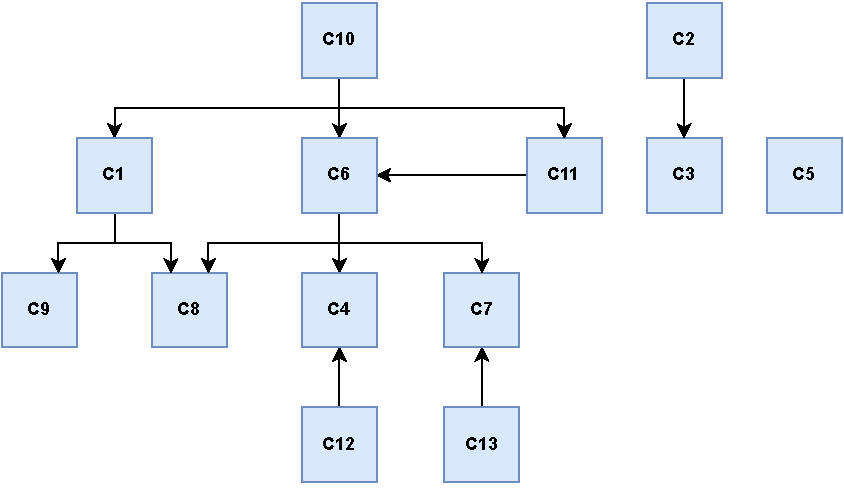
\includegraphics[width=0.87\linewidth]{figures/concept2concept.pdf}
    \caption[Dependencies between Conceptual Models]{Dependencies between
        Conceptual Models (Section~\ref{sec_conceptual})}
    \label{fig:conceptualdependencies}
\end{figure}
\vspace*{\fill}

\vspace*{\fill}
\begin{figure}[tbh]
    \centering
    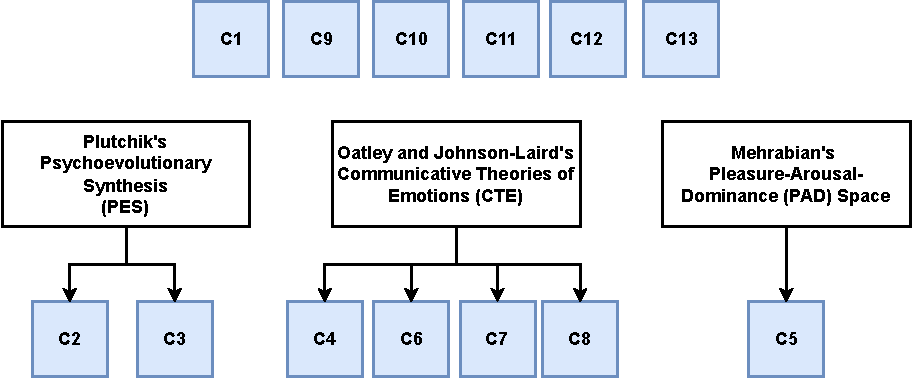
\includegraphics[width=\linewidth]{figures/theories2concept.pdf}
    \caption[Conceptual Model Dependencies on Affective
    Theories/Models]{Conceptual Model Dependencies on Affective Theories/Models
    (Section~\ref{sec_conceptual})}
    \label{fig:theories2conceptual}
\end{figure}
\vspace*{\fill}

\begin{figure}[tbh]
    \centering
    \includegraphics[height=0.96\textheight]{figures/assumptions2All.pdf}
    \caption[Dependencies on Assumptions]{Dependencies on Assumptions (Orange)
    (Section~\ref{sec_assumptions})}
    \label{fig:A2All}
\end{figure}

\begin{landscape}
    \begin{figure}[tbh]
        \centering
        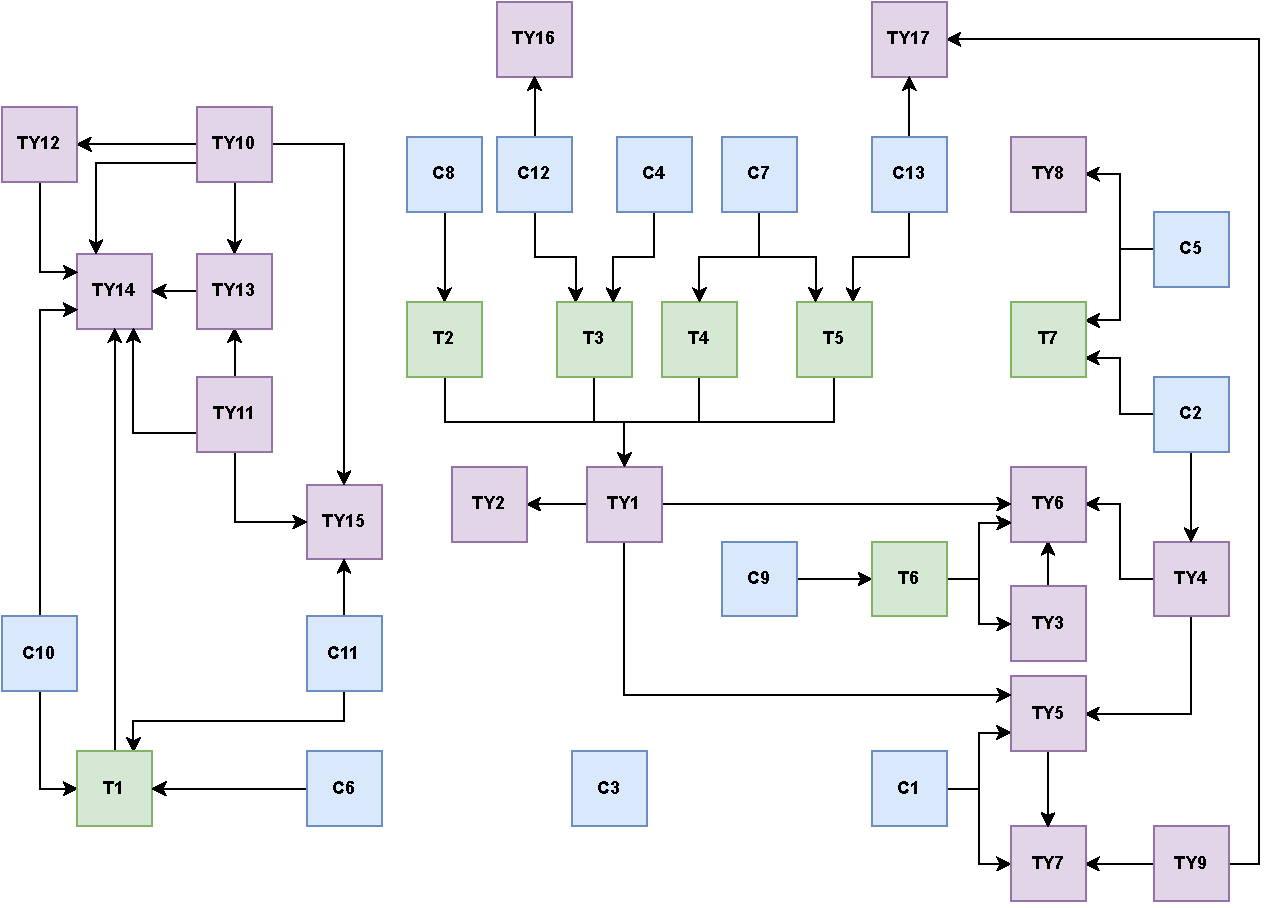
\includegraphics[width=\linewidth]{figures/concept2types_revised.pdf}
        \caption[Traceability between Theoretical Models and Data Types, and
        their dependencies on Conceptual Models]{Traceability between
        Theoretical Models (Green) and Data Types (Purple), and their
        dependencies on Conceptual Models (Blue)
        (Sections~\ref{sec_theoretical}, \ref{sec_typedefs},
        and~\ref{sec_conceptual})}
        \label{fig:C2TY}
    \end{figure}
\end{landscape}

\begin{landscape}
    \begin{figure}[tbh]
        \centering
        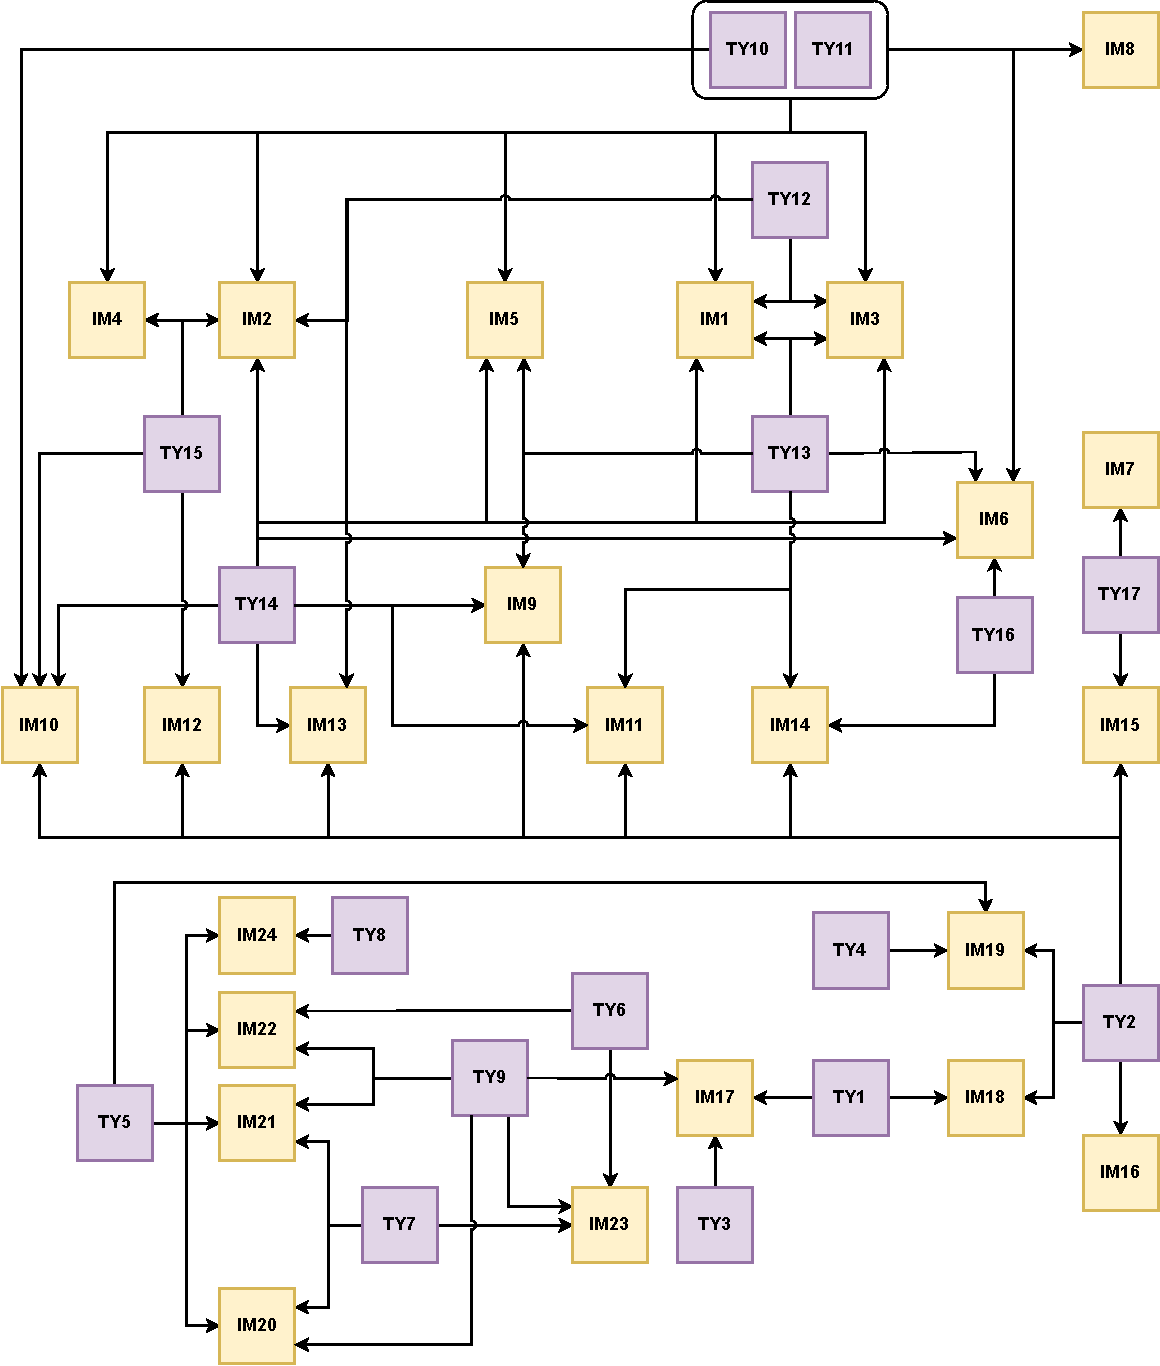
\includegraphics[width=0.88\linewidth]{figures/types2instance.pdf}
        \caption[Instance Models and their Dependencies on Theoretical Models
        and Data Types]{Instance Models (Yellow) and their Dependencies on
        Theoretical Models (Green) and Data Types (Purple)
        (Sections~\ref{sec_theoretical}, \ref{sec_typedefs},
        and~\ref{sec_instance})}
        \label{fig:T-TY2IM}
    \end{figure}
\end{landscape}

\vspace*{\fill}
\begin{figure}[tbh]
    \centering
    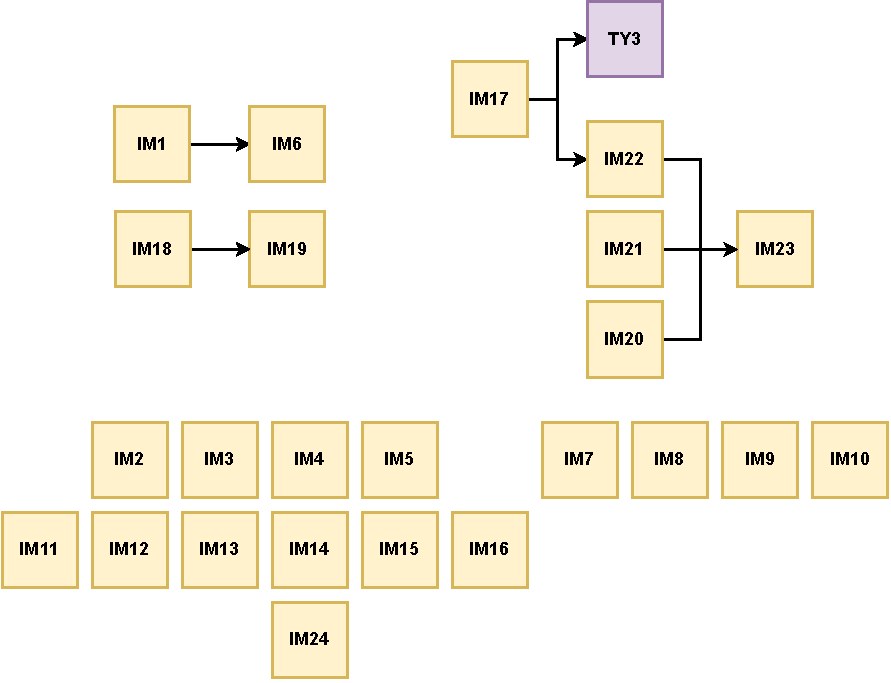
\includegraphics[width=0.5\linewidth]{figures/instance2instance.pdf}
    \caption[Dependencies between Instance Models]{Dependencies between
        Instance Models (Section~\ref{sec_instance})}
    \label{fig:IM}
\end{figure}
\vspace*{\fill}

\begin{figure}[tbh]
    \centering
    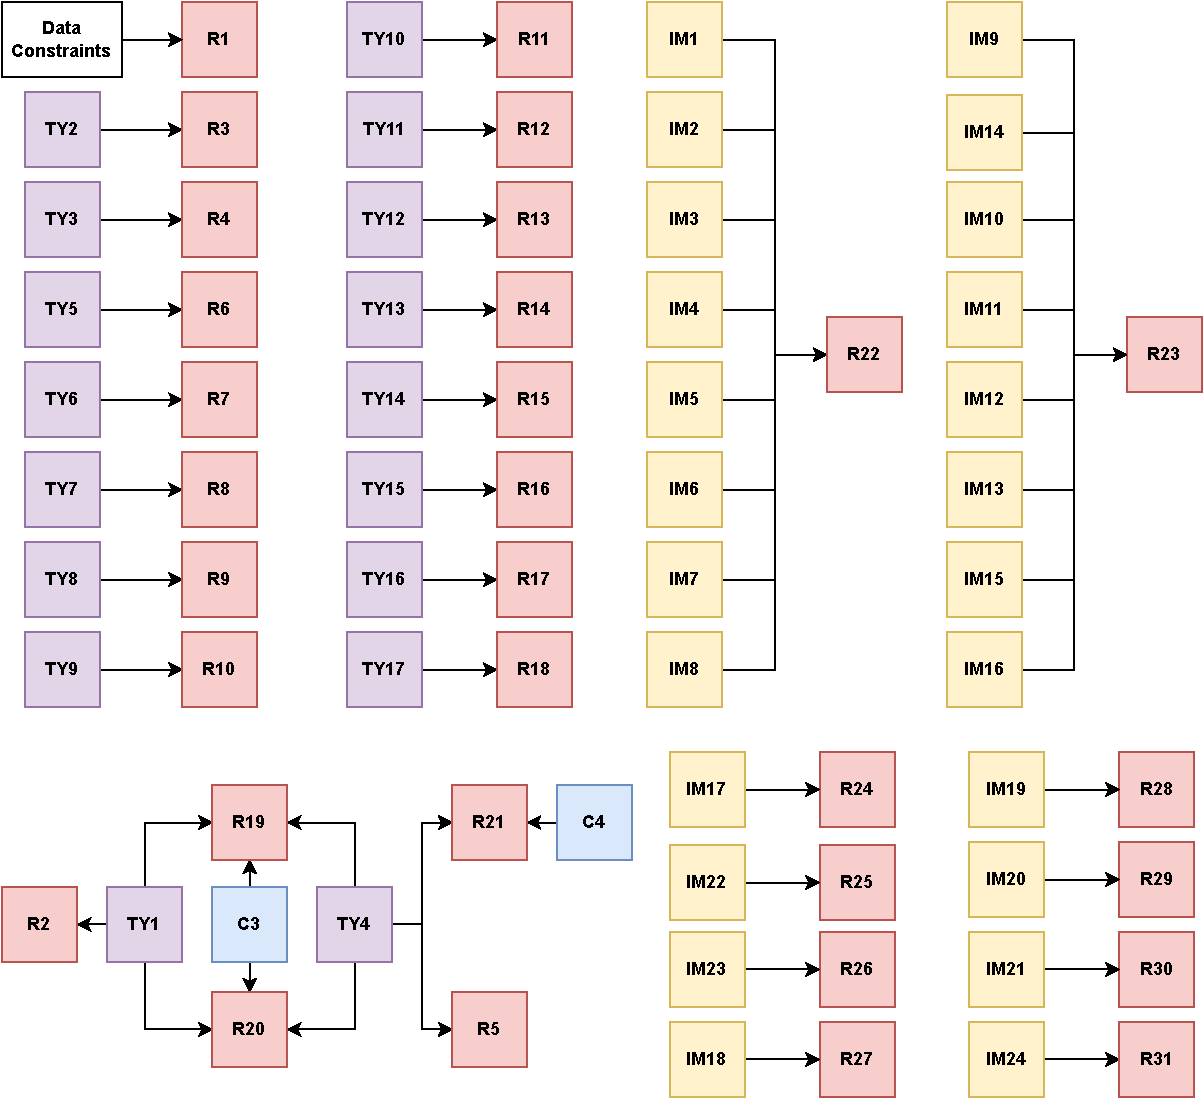
\includegraphics[width=\linewidth]{figures/reqs2All.pdf}
    \caption[Functional Requirements and their Dependencies on Conceptual
    Models, Data Types, Instance Models, and Data Constraints]{Functional
    Requirements (Red) and
    their Dependencies on Conceptual Models (Blue), Data Types (Purple),
    Instance Models (Yellow), and Data Constraints
    (Sections~\ref{sec_conceptual}, \ref{sec_typedefs}, \ref{sec_instance},
    \ref{sec_DataConstraints}, and \ref{sec_functionalreqs})}
    \label{fig:M2R}
\end{figure}

    \clearpage

    \bibliographystyle {ACM-Reference-Format}
    \bibliography
    {../../refs/references_documentation, ../../refs/references,
    ../../refs/references_psych, ../../refs/references_gamedesign,
    ../../refs/references_definitions, ../../refs/references_media,
    ../../refs/references_SEPerspective, ../../refs/references_Geneva}

    \clearpage

    \begin{appendix}

        \section{Notes On Emotion Theories With Respect to High-Level Requirements and
Emotion Theories}\label{chapter:reqsTheoryNotes}
% This is a copy of the information from the thesis, modified to work with the
%SRS

These are the notes created about emotion theories with respect to high-level
requirements during analysis (Section~\ref{sec_theories}).
Tables~\ref{tab:theory-req-sys-summary-flexibility},
\ref{tab:theory-req-sys-summary-easeofuse},
\ref{tab:theory-req-comp-summary-flexibility}, and
\ref{tab:theory-req-comp-summary-easeofuse} summarize the resulting scores.

A reminder that the scores are somewhat subjective, and depend on one's
understanding of the requirements and current state of emotion literature.

\subsection{Discrete Theories}
The discrete theories are the most likely candidates for satisfying high-level
requirements that depend on understanding what emotion an NPC has, as this is
their core focus. This includes the flexibility requirements for
\textit{Allowing the Integration of New Components} (\ref{flexNew}) and
\textit{Choosing Which NPC Emotions to Use} (\ref{flexEm}), and the ease-of-use
requirements for \textit{Having a Clear API (Output)} (\ref{easeAPI}) and
\textit{Showing That Emotions Improve the Player Experience} (\ref{easePX}).

\subsubsection{Flexibility: Allowing the Integration of New Components
    (\ref{flexNew})}
All three discrete theories provide variable levels of native support for
personality, but only Plutchik does not touch on mood. None of them touch on
core affect.

\begin{itemize}
    \item \textbf{Ekman \& Friesen} (\weak)
    \begin{itemize}
        \item Moods and personality are inferred from emotion
        signals (e.g. many \textit{Joy}-related signals could suggest a
        cheerful mood)~\citep[p.~48, 55--56]{ekman1999basic}

        \item Little information beyond these definitions $\rightarrow$
        developers would need to create patterns of emotions for each mood and
        trait, could become too time consuming and error-prone

        \item No coverage of Core Affect, Personality and Mood are error-prone
        and time consuming
    \end{itemize}

    \item \textbf{Izard} (\weak)
    \begin{itemize}
        \item Natively accounts for personality
        (\citepg{izard2000motivational}{253--254}; \citepg{izard1977human}{44})
        \begin{itemize}
            \item Emergent phenomena that begins at birth and develops as the
            individual interacts with their environment

            \item Treated as a product of emotions associated with patterns in
            perception, cognition, and behaviour

            \item [$\rightarrow$] Requires developers to create patterns for
            each personality trait, which is likely to be too time consuming
            and error-prone
        \end{itemize}

        \item Seems to acknowledge two definitions of mood
        \begin{itemize}
            \item Defined as a ``continuing total life condition'' similar to
            what he calls an emotion trait, or tendencies towards certain
            emotion experiences~\citep[p.~17, 171]{izard1991psychology}
            $\rightarrow$ in the view of stable traits and fluid states,
            conceptualization appears to be closer to personality than mood

            \item As a state, defined as an enduring emotion state that is too
            mild to enter conciousness but can influence mental health and
            bodily systems, such as the immune
            system~\citep[p.~21]{izard1991psychology} $\rightarrow$ closer to
            working definition of mood in \progname{}'s context

            \item [$\rightarrow$] could be realized as a timed function that
            monitors an NPC's emotion state and acts on those that have not
            surpassed a given threshold (minimal effort to implement)
        \end{itemize}

        \item No coverage of Core Affect, Mood requires minimal effort,
        Personality is error-prone and time consuming
    \end{itemize}

    \item \textbf{Plutchik} (\good)
    \begin{itemize}
        \item Natively accounts for personality
        \begin{itemize}
            \item Connects its emotion circumplex directly to a
            circumplex of personality traits\footnote{The assumption that
                the circumplexes can be connected this way might be naive. They
                might be unique to the modelled domain rather than showing
                similarities across them~\citep[p.~815]{feldman1995variations}.}
            \citep[p.~27--28]{plutchik1997circumplex} $\rightarrow$ could
            mechanize with a simple weighting mechanism such that emotions are
            easier or harder to elicit

            \item Built around a layperson's understanding of personality
            $\rightarrow$ upholds the \textit{Hiding the Complexity of Emotion
                Generation} (\ref{easeHide}) requirement
        \end{itemize}

        \item circumplex is a way to incorporate a model of mood
        \begin{itemize}
            \item Agreement that it can be represented by an elliptical
            circumplex with arousal as the shorter
            dimension~\citep[p.~806, 812, 814]{feldman1995variations}

            \item Could add an additional element such that the length of the
            arousal dimension changes with context $\rightarrow$ afford
            more creative freedom than a fixed model

            \item Can uphold the \textit{Hiding the Complexity of Emotion
                Generation} requirement (\ref{easeHide}) with a well-designed
            interface, with details available for advanced users
        \end{itemize}

        \item Dimensional nature of theory could aid in a non-native
        representing core affect $\rightarrow$ could map the intensity
        dimension to arousal and the relative positions of an emotion to
        some anchor points as \textit{valence}
        \begin{itemize}
            \item Mapping might not be understandable due to debate about the
            \textit{valence} of \textit{Surprise} and its relation to
            \textit{Anticipation}~\citep[p.~98]{susanto2020hourglass}
            $\rightarrow$ concessions could be made, such as listing some
            categories as zero \textit{valence}, since \progname{} is
            unconcerned with realism

            \item Can uphold the \textit{Hiding the Complexity of Emotion
                Generation} requirement (\ref{easeHide}) with a well-designed
            interface, with details available for advanced users
        \end{itemize}

        \item Ability to build \textit{some} type of Core Affect and Mood
        representation on top of existing theory, Personality native to theory
        and built on a layperson's perspective
    \end{itemize}
\end{itemize}

\subsubsection{Flexibility: Choosing What Emotions the NPC can Have
(\ref{flexEm})}
Within each discrete theory's set of emotions, it would be easy to exclude any
of them if they are not needed. However, \textit{adding} more emotions to a set
is less clear cut. There does not seem to be any convincing empirically
validated or verifiable rules for creating ``non-basic'' emotions in discrete
theories~\citep[p.~6]{ortony2021all}. This does not impact \progname{} because
it does not need to replicate true affective phenomena---it need only produce
convincing results.

\begin{itemize}
    \item \textbf{Ekman \& Friesen} (\weak)
    \begin{itemize}
        \item Do not believe that there are ``non-basic''
        emotions~\citep[p.~55, 57]{ekman1999basic}
        \begin{itemize}
            \item Each emotion represents a family of related states that share
            a theme, and variations between members are the result of learning

            \item [$\rightarrow$] Requires developers to either associate
            different situations for the desired variations manually or create
            a learning mechanism to create them as the NPC interacts with the
            game environment

            \item Unideal $\rightarrow$ Could be difficult to adapt this kind
            of system to simple games, violating the \textit{Ability to Operate
                on Different Levels of NPC Complexity} requirement
            (\ref{flexComplex}); requires some knowledge of psychology and
            neuroscience, violating the \textit{Hiding the Complexity of
                Emotion Generation} (\ref{easeHide}) requirement
        \end{itemize}

        \item Facial expressions can be blends of prototypical primary
        ones~\citep[p.~69]{ekman2007emotions}
        \begin{itemize}
            \item Step removed from the emotion generation process, and would
            likely happen in an emotion expression component

            \item Would need to translate the blended expression into an
            emotion to use it for emotion generation $\rightarrow$ feasible,
            but error-prone, method as facial expression interpretations can be
            subjective
        \end{itemize}

        \item No ``non-basic'' emotions, translating from facial expressions is
        error-prone
    \end{itemize}

    \item \textbf{Izard} (\disqualified)
    \begin{itemize}
        \item ``New emotions'' are the product of affective-cognitive
        structures~\citep[p.~564--565]{izard1992basic}
        \begin{itemize}
            \item Association of primary emotion patterns or clusters with
            images, thoughts, and memories

            \item [$\rightarrow$] Requires developers to either create these
            structures manually or create a learning mechanism to create them
            as the NPC interacts with the game environment

            \item Unideal $\rightarrow$ Same reasons as Ekman \& Friesen,
            violating both the \textit{Ability to Operate on Different Levels
                of NPC Complexity} and \textit{Hiding the Complexity of Emotion
                Generation} requirements (\ref{flexComplex}, \ref{easeHide})
        \end{itemize}

        \item Difficult to adapt to different NPC complexities, requires
        knowledge for connecting emotions to cognitive patterns
    \end{itemize}

    \item \textbf{Plutchik} (\strong)
    \begin{itemize}
        \item One of the better developed theories of emotion mixes
        (\citepg{ledoux1996emotional}{113}; \citepg{ortony2021all}{3, 5})

        \item Might be the only discrete theory to focus on this aspect of the
        ``primary'' emotions~\citep[p.~47]{ekman1999basic}

        \item Colour wheel analogy uses concepts and terms that are generally
        understood by laypeople $\rightarrow$ does not require any knowledge of
        the theory to use
        \begin{itemize}
            \item Lacks clarity about technical rules for combining emotions
            (\citepg{johnson1992basic}{208--209}; \citepg{ortony2021all}{5})
            \textbf{BUT} laypeople tend to attribute the same underlying
            primary emotions to named emotions outside the primary
            set~\citep[p.~204--205]{plutchik1984emotions}

            \item [$\rightarrow$] Implies that a game developer can apply their
            own experiences when deciding how to represent a new emotion with
            the Plutchik circumplex
        \end{itemize}

        \item Ability to build additional emotions from existing set, based on
        a layperson's understanding of emotions and their combinations
    \end{itemize}
\end{itemize}


\subsubsection{Ease-of-Use: Having a Clear API (Output)  (\ref{easeAPI})}
The discrete theories are generally easy for laypeople to understand. All three
theories connect their emotions to distinctive behaviours that can be applied
to situations of variable complexity. This makes for a clean output API,
providing an emotion category that developers can attach to ``buckets'' of
related behaviours and expressions that are ``familiar''.

\begin{itemize}
    \item \textbf{Ekman \& Friesen} (\strong)
    \begin{itemize}
        \item Have publications that are meant for the general public (e.g.
        \cite{ekman2007emotions}) $\rightarrow$ accessible to laypeople

        \item Use of facial expressions is a helpful tool for conveying meaning
        about their primary emotions
    \end{itemize}

    \item \textbf{Izard} (\weak)
    \begin{itemize}
        \item Gains understandability by connecting its emotions to facial
        expressions, although some emotions are not connected to one

        \item [$\rightarrow$] Weakens its usability, as some developers might
        actively avoid the emotions that cannot be readily represented on the
        face
    \end{itemize}

    \item \textbf{Plutchik} (\good)
    \begin{itemize}
        \item Construction based on similarities and differences between
        affective terms as they are understood in (English) language
        $\rightarrow$ can help developers understand each emotion based on
        their understanding of the word's meaning and its relative position to
        other emotion words on the circumplex

        \item Each primary emotion is also connected to an intended behaviour
        pattern, like rejection and
        exploration~\citep[p.~202]{plutchik1984emotions}
        \begin{itemize}
            \item  Addresses problems of ``missing'' facial expressions with
            characteristic or typical behaviours
            (\citepg{julle2020there}{20--21};
            \citepg{schindler2013admiration}{101})

            \item [$\rightarrow$] Could help developers conceptualize what each
            emotion could look and act like, can include facial expressions
        \end{itemize}

        \item Does not directly benefit from assigned facial expressions, but
        some connections could be made with Ekman \& Friesen and Izard
        (Table~\ref{tab:discreteEmotions}) $\rightarrow$ understanding of
        emotion terms and associated behaviours is not as ``clear cut''
    \end{itemize}
\end{itemize}

\begin{table}[!tb]
    \begin{center}
        \renewcommand{\arraystretch}{1.2}
        \begin{threeparttable}
            \caption{Primary Emotions in Discrete Theories}
            \label{tab:discreteEmotions}

            \begin{tabular}{lccc}
                \toprule
                \textbf{Emotion} & {\begin{tabular}[c]{@{}c@{}}\textbf{Ekman \&
                            Friesen} \\
                        \textbf{\citep{ekman2007emotions}}\end{tabular}} &
                \textbf{\citet{izard1993stability}} &
                \textbf{\citet{plutchik1997circumplex}} \\ \hline

                \rowcolor[gray]{0.9}Happiness/Enjoyment/Joy\textsuperscript{\large\Jupiter\Pluto}
                & \checkmark & \checkmark & \checkmark \\

                Sadness\textsuperscript{\large\Jupiter\Pluto} & \checkmark &
                \checkmark & \checkmark \\

                \rowcolor[gray]{0.9}Fear\textsuperscript{\large\Jupiter\Pluto}
                & \checkmark & \checkmark & \checkmark \\

                Anger\textsuperscript{\large\Jupiter\Pluto} & \checkmark &
                \checkmark & \checkmark \\

                \rowcolor[gray]{0.9}Surprise\textsuperscript{\large\Jupiter\Pluto}
                & \checkmark & \checkmark & \checkmark \\

                Disgust\textsuperscript{\large\Jupiter\Pluto} & \checkmark &
                \checkmark &
                \checkmark \\

                \rowcolor[gray]{0.9}Contempt\textsuperscript{{\normalsize\Moon}{\large\Pluto}}
                & \checkmark & \checkmark &
                {\small\textpmhg{\Hibp}} \\

                Interest\textsuperscript{\large\Pluto} &  & \checkmark &
                \checkmark \\

                \rowcolor[gray]{0.9}Guilt\textsuperscript{\large\textpmhg{\Hl}}
                 & & \checkmark & {\small\textpmhg{\Hibp}} \\

                Shame\textsuperscript{\large\Pluto} &  & \checkmark &
                {\small\textpmhg{\Hibp}} \\

                \rowcolor[gray]{0.9}Shyness\textsuperscript{\large\Pluto}
                &  & \checkmark & \\

                Acceptance\textsuperscript{{\large\textpmhg{\Hl}}\textpmhg{\Hi}}
                &  & & \checkmark \\
                \hline

                \bottomrule

            \end{tabular}

            \begin{tablenotes}
                \footnotesize
                \vspace*{2mm}

                \item []{\Large\Jupiter} \textit{Associated with a facial
                    expression by \citet{ekman2003unmasking}.}

                \item []{\Large\Pluto} \textit{Associated with a facial
                    expression by \citet[p.~236--237]{izard1971face},
                    \citet[p.~85--91]{izard1977human}.}

                \item []{\normalsize\Moon} \textit{Associated with a facial
                    expression by \citet[p.~184--186]{ekman2007emotions}.}

                \item []{\normalsize\textpmhg{\Hibp}} \textit{As a mixture of
                    the primary emotions.}

                \item []{\normalsize\textpmhg{\Hl}} \textit{Might not have a
                characteristic expression
                    (\citepg{keltner1996evidence}{155};
                    \citepg{schindler2013admiration}{106}), but artistic
                    renditions of facial expressions exist (e.g.
                    \citet{lebrun1760admiration}).}

                \item []{\normalsize\textpmhg{\Hi}} \textit{Plutchik is noted
                as the only researcher to consider \textit{Adoration}---the
                highest intensity of \textit{Acceptance}---a primary
                emotion~\citep[p.~87--88]{schindler2013admiration}.}

                \vspace*{-7mm}
            \end{tablenotes}
        \end{threeparttable}%
    \end{center}
\end{table}

\subsubsection{Ease-of-Use: Showing that Emotions Improve the Player Experience
    (\ref{easePX})}
Like the \textit{Having a Clear API (Output)} requirement  (\ref{easeAPI}),
discrete theories are generally understandable by laypeople. This helps
identify ways to design studies to evaluate and ways to build the player
experience.

\begin{itemize}
    \item \textbf{Ekman \& Friesen} (\good)
    \begin{itemize}
        \item Emotions could be directly connected to an expression module
        built on the Facial Action Coding System (FACS), which is part of the
        theory itself~\citep{facs}

        \item Players could report on their experiences based on NPC
        expressions $\rightarrow$ relatively easy to test how emotions impact a
        player, but limited to facial expressions alone
    \end{itemize}

    \item \textbf{Izard} (\good)
    \begin{itemize}
        \item Considerable overlap between Ekman \& Friesen and Izard regarding
        facial expressions~\citep[p.~3]{ekman2007emotions} $\rightarrow$ could
        be connected to an emotion expression component built on FACS, probably
        with minimal effort

        \item Players could report on their experiences based on NPC
        expressions $\rightarrow$ relatively easy to test how emotions impact a
        player, but limited to facial expressions alone
    \end{itemize}

    \item \textbf{Plutchik} (\good)
    \begin{itemize}
        \item Could be connected to facial expressions, but there is no obvious
        match for \textit{Acceptance} emotion type

        \item Associates each emotion with a behaviour that could be applied to
        a number of actions and expressions that an NPC could need
        $\rightarrow$ design studies around these behaviour classes

        \item Players could report on their experiences based on NPC
        expressions $\rightarrow$ relatively easy to test how emotions impact a
        player, but likely an element of subjectivity in matching behaviours to
        meaning
    \end{itemize}
\end{itemize}

\subsubsection{Examining the Remaining Requirements}
The absence of a defined emotion elicitation tasks in the discrete theories is
a double-edged sword---some requirements are trivial to satisfy, while others
are impossible. The lack of elicitation processes makes it impossible for
discrete theories to satisfy most task-related requirements---they simply do
not exist. This means that they \textit{cannot} be categorized for the
component-level requirements
(Tables~\ref{tab:theory-req-comp-summary-flexibility} and
\ref{tab:theory-req-comp-summary-easeofuse}). For the remaining system-level
requirements (Tables~\ref{tab:theory-req-sys-summary-flexibility} and
\ref{tab:theory-req-sys-summary-easeofuse}), the theories satisfy the
requirements in similar ways, so they are examined as a single unit.
\begin{itemize}
    \item \textit{Flexibility: Independence from an Agent Architecture
        (\ref{flexArch})} (\good)
    \begin{itemize}
        \item No specific tasks $\rightarrow$ effectively architecture-agnostic

        \item Only require processes that satisfy input and output requirements
    \end{itemize}

    \item \textit{Flexibility: Allowing Developers to Specify How to Use
        Outputs (\ref{flexOut})} (\good)
    \begin{itemize}
        \item No specific tasks $\rightarrow$ affords flexibility for
        specifying how to use \progname{}'s outputs

        \item Theoretically could hook up any process to \progname{} using the
        emotions as ``buckets'' for collecting related behaviours
    \end{itemize}

    \item \textit{Flexibility: Ability to Operate on Different Levels of NPC
        Complexity (\ref{flexComplex})} (\good)
    \begin{itemize}
        \item Could add processes and parameters as needed $\rightarrow$ does
        not affect core \progname{} processes
    \end{itemize}

    \item \textit{Flexibility: Be Efficient and Scalable (\ref{flexScale})}
    (\good)
    \begin{itemize}
        \item Could add processes and parameters as needed $\rightarrow$ does
        not affect core \progname{} processes
    \end{itemize}

    \item \textit{Ease-of-Use: Providing Examples of Novel Game Experiences
        (\ref{easeNovel})} (\weak)
    \begin{itemize}
        \item No immediately obvious features for novel game mechanics,
        challenges, or other elements
    \end{itemize}
\end{itemize}

\subsection{Dimensional Theories}
The dimensional theories are the most likely candidates for satisfying
requirements related to CME expansion, as they aim to discover the structure of
emotion and how they relate to other mental
states (\citepg{reisenzein2013computational}{250};
\citepg{broekens2021emotion}{353}). This mainly concerns the flexibility
requirements for \textit{Allowing the Integration of New Components}
(\ref{flexNew}) and \textit{Choosing What Emotions the NPC can Have}
(\ref{flexEm}).

For this analysis, the V-A model is treated as a circumplex as it is a
reasonable representation of affective
states~\citep[p.~296]{remington2000reexamining}, and is more consistent with
affective structure~\citep[p.~12]{barrett1999structure}. The circumplex
also tends to form regardless of the data collected, research domain, and
analysis~\citep[p.~211]{russell1997how}. This representation is not perfect.
There are still issues, such as inclusion/exclusion of terms, self-report
weaknesses, and the effect of context on state
positions~\citep[p.~298]{remington2000reexamining}. However, it also provides
more structure to an otherwise two-dimensional and nebulous space.

\subsubsection{Flexibility: Choosing What Emotions the NPC can Have
(\ref{flexEm})}
Neither V-A or PAD strictly enforce the inclusion of specific emotion types.
Instead, the use of dimensions allows for an infinite number of affective
states. While this trivially supports the ability to \textit{Choose What
    Emotions the NPC can Have} (\ref{flexEm}), it might not be practical for
\progname{} on its own. Instead, adding specific emotions is guided by point
locations representing named emotions. This removes the burden of deciding
where an emotion is located in dimensional space from game designers.

\begin{itemize}
    \item \textbf{V-A} (\weak)
    \begin{itemize}
        \item Space represented by \textit{valence} and \textit{arousal} only
        represents part of an emotion episode (\citepg{yik2002relating}{90};
        \citepg{roseman2011emotional}{441}; \citepg{lisetti2015and}{97})

        \item Unideal $\rightarrow$ some emotions, like \textit{Anger} and
        \textit{Fear}, are difficult to differentiate without additional
        information
        \begin{itemize}
            \item Might be some of the most common emotions that a game
            designer will use $\rightarrow$ could be the \textit{only} two
            emotions required in some games (e.g. NPCs in oppositional
            First Person Shooters (FPSs) due to the game's pace and the
            limited time and ways that players interact with them)
        \end{itemize}

        \item Adding new emotions cannot be adequately contained in V-A
    \end{itemize}

    \item \textbf{PAD} (\good)
    \begin{itemize}
        \item Accompanied by a list of 151 emotion
        labels~\citep[p.~42--45]{mehrabian1980basic} identified from empirical
        data $\rightarrow$ notes their average location in PAD space and the
        standard deviation in the data

        \item List is still finite and cannot account for cultural differences,
        might not cover all of the affective states that a game designer needs
        $\rightarrow$ list is long enough that there is a reasonable chance
        that a game designer can find all the affective state labels that they
        require

        \item Prone to interpretation errors, as the designer's definition and
        the definition used to locate points in PAD space might not be the same
        $\rightarrow$ designers can make their own judgements of the
        suitability of a term based on its coordinates, potentially violating
        \textit{Hiding the Complexity of Emotion Generation} (\ref{easeHide})
    \end{itemize}
\end{itemize}

\subsubsection{Flexibility: Allowing the Integration of New Components
(\ref{flexNew})}
Both V-A and PAD can trivially represent core affect, as they both natively
include the dimensions of \textit{valence} and arousal. Like Plutchik, both
dimensional theories could also model mood as an elliptical circumplex with
relative ease. Unlike Plutchik, this mapping is native due to the presence of
both a \textit{valence}/\textit{pleasantness} and arousal dimension. This only
leaves an evaluation of the ability to represent personality in V-A and PAD.

The dimensional theories seem to have variable levels of built-in support for
representing personality. This analysis focuses on support for the Five-Factor
Model OCEAN\footnote{Defined as ``psychological entities with causal
    force''~\citep{ffmdef}. Although they have the same dimensions, this differs
    from the Big Five Model, which ``views the five personality dimensions as
    descriptions of behaviour and treats the five-dimensional structure as a
    taxonomy of individual differences''.} personality
traits~\citep{costa1992normal}. With research ongoing in personality
psychology, there is still a good consensus on the usefulness of OCEAN as a
descriptive model (\citepg{yik2002relating}{100--101};
\citepg{raad2002big}{3}). OCEAN has, arguably, also become known among the
general populace as a personality profile tool due to its accessible
language~\citep[p.~1]{raad2002big} and use in career counselling
(\citepg{costa1995persons}{135}; \citeg{howard1995big};
\citepg{hurtado2019five}{528}). This familiarity makes it ideal for
\progname{}, which cannot assume that a user will have an academic
understanding of psychology. For game design, the OCEAN model will also likely
prove convenient for defining NPC personalities, as \citet{costa1992normal}
provide a questionnaire consisting of five-point Likert scales representing
statement agreement to measure how each factor contributes to personality. It
has also been translated to several languages~\citep[p.~84]{yik2002relating}.
This implies that a simple tool presenting game designers with the
questionnaire is sufficient for defining a new NPC personality in \progname{}
with OCEAN traits.

\begin{itemize}
    \item \textbf{V-A} (\strong)
    \begin{itemize}
        \item Relating OCEAN personality traits with circumplex
        structures is more consistent than simple structures $\rightarrow$ two
        structures have close-fitting probability plots supporting an ideal
        circumplex structure and the third has convincing and
        serviceable, but less satisfactory, probability plot~\citep[p.~84--87,
        90]{gurtman1997studying}
        \begin{itemize}
            \item Some evidence that the interpersonal traits of Extroversion
            and Agreeableness are best described with a circumplex
            $\rightarrow$ Extroversion can be related to the \textit{valence}
            dimension~\citep[p.~590, 593]{mccrae1989structure}

            \item Extroversion/Neuroticism $\rightarrow$ represents the
            affective plane~\citep[p.~84--87, 90]{gurtman1997studying}

            \item Unnamed or ``mixed'' Agreeableness/Neuroticism
            plane~\citep[p.~84--87, 90]{gurtman1997studying}

            \item All three planes can be layered over each other in the polar
            coordinate system~\citep[p.~84--87, 90]{gurtman1997studying}

            \item Does not appear to be support for Openness or
            Conscientiousness~\citep[p.~84--87, 90]{gurtman1997studying}
        \end{itemize}

        \item Alternate hypothesis puts OCEAN traits as points on the
        circumplex $\rightarrow$ a high value in a trait implies a higher
        tendency to experience the type of affect represented in
        the same space~\citep[p.~94--96]{yik2002relating}
        \begin{itemize}
            \item Locates the angles for each trait in five
            languages---English, Spanish, Korean, Chinese, and Japanese

            \item Configuration option $\rightarrow$ pre-build some cultural
            differences into \progname{}
        \end{itemize}
    \end{itemize}

    \item \textbf{PAD} (\strong)
    \begin{itemize}
        \item Personality\footnote{Mehrabian refers to \textit{emotional
                traits} or \textit{temperament}. Since he defines them as
                ``...stable
            over periods of years or even a
            lifetime''~\citep[p.~262]{mehrabian1996pleasure} and temperament is
            a
            biologically-based bias in personality
            development~\citep{oxfordTemperament}, they are assumed to be
            equivalent to personality traits in \progname{}.} can be inferred by
        averaging an individual's emotional states across a representative
        sample of day-to-day situations~\citep[p.~262]{mehrabian1996pleasure}

        \item As traits, the PAD dimensions were found to be a good base
        description of personality~\citep[p.~64]{mehrabian1980basic}

        \item  Other personality scales are represented as linear combinations
        of the three dimensions~\citep[p.~267]{mehrabian1996pleasure}, forming
        a line through the space
        \begin{itemize}
            \item Provides lines estimates for the OCEAN personality
            traits\footnote{\textit{Trait Sophistication} is assumed to be
                equivalent to \textit{Trait
                    Openness}~\citep[p.~826--827]{mccrae1997conceptions}.} in
                    terms of
            \textit{pleasure}, arousal, and
            \textit{dominance}~\citep[p.~91
            Eq.~11C--13C]{mehrabian1996analysis}, and from the dimensions to
            PAD space~\citep[p.~90 Eq.~1D--5D]{mehrabian1996analysis}

            \item Gender agnostic~\citep[p.~89]{mehrabian1996analysis}
            $\rightarrow$ removes a layer of complexity that one might consider
            when adding the OCEAN model of personality to \progname{}
        \end{itemize}
    \end{itemize}
\end{itemize}

\subsubsection{Examining the Remaining Requirements}
Dimensional theories are  similar to the discrete theories in that they have no
defined emotion elicitation tasks, so they are also unable to satisfy the
component-level requirements
(Tables~\ref{tab:theory-req-comp-summary-flexibility} and
\ref{tab:theory-req-comp-summary-easeofuse}). However, for the remaining
system-level requirements (Tables~\ref{tab:theory-req-sys-summary-flexibility}
and \ref{tab:theory-req-sys-summary-easeofuse}), the dimensional theories do
not necessarily satisfy the same requirements as discrete theories. Again, the
dimensional theories satisfy the requirements in similar ways, so they are
examined as a single unit.
\begin{itemize}
    \item \textit{Flexibility: Independence from an Agent Architecture
        (\ref{flexArch})} (\good)
    \begin{itemize}
        \item Coordinate space that does not depend on its surrounding
        environment $\rightarrow$ effectively architecture-agnostic

        \item Only require processes that satisfy input and output requirements
    \end{itemize}

    \item \textit{Flexibility: Allowing Developers to Specify How to Use CME
        Outputs (\ref{flexOut})} (\strong)
    \begin{itemize}
        \item Numerical representation $\rightarrow$ easy to pipe them to other
        computational processes, such as facial expression generation and
        decision-making

        \item Potential to violate \textit{Having a Clear API (Output)}
        (\ref{easeAPI}) $\rightarrow$ resolve by providing alternate
        definitions of the dimensions that are easier to understand for
        non-experts
    \end{itemize}

    \item \textit{Flexibility: Ability to Operate on Different Levels of NPC
        Complexity} (\ref{flexComplex}) (\weak) AND \textit{Flexibility: Be
        Efficient and Scalable} (\ref{flexScale})
    (\weak)
    \begin{itemize}
        \item Numerical representation could satisfy these requirements
        $\rightarrow$ requires one of:
        \begin{itemize}
            \item Developers to have some understanding of what the dimensions
            mean and how different factors impact them $\rightarrow$ violates
            \textit{Hiding the Complexity of Emotion Generation}
            (\ref{easeHide})

            \item Providing alternate definitions of the dimensions that are
            easy to understand as with \textit{Allowing Developers to Specify
                How to Use CME Outputs} (\ref{easeAPI}) $\rightarrow$ potential
                to
            violate \textit{Hiding the Complexity of Emotion Generation}
            (\ref{easeHide})
        \end{itemize}
    \end{itemize}

    \item \textit{Ease-of-Use: Having a Clear API (Output) (\ref{easeAPI})}
    (\weak)
    \begin{itemize}
        \item Output API has three numerical components $\rightarrow$ requires
        developers to know how each dimension affects NPC behaviours

        \item Inference on quantities like \textit{pleasantness}
        (\textit{valence}) and \textit{excitement} (arousal) likely not as
        automatic as identifying \textit{Joy} and \textit{Fear}
        \begin{itemize}
            \item Could minimize problem with a circumplex structure

            \item Disagreements between different models as to where certain
            data points should be~\citep[p.~287]{remington2000reexamining}
            $\rightarrow$ could reduce the psychological validity of \progname{}
        \end{itemize}
    \end{itemize}

    \item \textit{Ease-of-Use: Showing that Emotions Improve the Player
        Experience (\ref{easePX})} (\good)
    \begin{itemize}
        \item Numerical representation with limited variables $\rightarrow$
        easy to manipulate in  experimental settings

        \item Might be difficult for future user study participants to answer
        questions about combinations of values $\rightarrow$ could use a proxy
        mapping values to affective labels
    \end{itemize}

    \item \textit{Ease-of-Use: Providing Examples of Novel Game Experiences
        (\ref{easeNovel})} (\good)
    \begin{itemize}
        \item Numerical representation $\rightarrow$ leverage as a game
        mechanic where players manipulate affective variables as they would
        other resources like character and item statistics~\citep[p.~292, 466,
        559--560, 578]{adams2014fundamentals}

        \item Can be implemented alongside similar mechanics (e.g. status
        attributes in Computer Role-Playing Games (CRPGs), character-related
        puzzles in adventure and social simulation games)
    \end{itemize}
\end{itemize}

\subsection{Appraisal Theories}
Due to their nature, the appraisal theories are the only ones that can satisfy
the \textit{component-level} requirements in addition to \textit{system-level}
ones.

\subsubsection{Flexibility: Independence From an Agent Architecture
    (\ref{flexArch})}
Appraisal theories are built on the assumption that cognition is essential in
emotion processes (\citepg{marsella2015appraisal}{55};
\citepg{broekens2021emotion}{354}), and that emotions \textit{about}
something that has been intentionally evaluated~\citep[p.~11]{ortony2021all}.
This prevents complete separation from agent architectures in general because
of the information required for the appraisal process. Therefore, the goal is
\textit{not} to identify theories that can exist independently of an external
system---it is to identify which theories are agnostic about what that
architecture is.

\begin{itemize}
    \item \textbf{Frijda} (\strong)
    \begin{itemize}
        \item Core process is an information processing
        system~\citep[p.~453--456]{frijda1986emotions} that begins with an
        encoding stage that tries to match incoming events with known types and
        their implications for causes and consequences
        \begin{itemize}
            \item Also need to encode actions to evaluate coping potential

            \item Matching process requires users to define event and action
            types, then tag relevant game elements with them
            \begin{itemize}
                \item Event types are tailored to the external architecture
                $\rightarrow$ affords maximal architecture independence
            \end{itemize}
        \end{itemize}

        \item Concerns are dispositions towards the achievement or
        non-achievement of situations that remain dormant as long as its
        satisfaction conditions are met~\citep[p.~335--336,
        466--467]{frijda1986emotions}
        \begin{itemize}
            \item Do not have to generate emotion from ``active'' pursuits
            alone (e.g. goals and motivations), can also be driven by events
            that just \textit{happen} that change a satisfaction condition

            \item [$\rightarrow$] Can account for a much wider range of events,
            supports independence from specific architectures and information
            structures
        \end{itemize}

        \item Action tendencies only specify \textit{what} type of action should
        happen, not \textit{how}~\citep[p.~70]{frijda1986emotions}
        \begin{itemize}
            \item Freedom to connect the actions represented in the
            architecture to any type of action readiness $\rightarrow$ separate
            process can decide which action to execute

            \item [$\rightarrow$] Can account for a much wider range of
            behaviours, supports independence from specific architectures and
            information structures
        \end{itemize}
    \end{itemize}

    \item \textbf{Lazarus} (\good)
    \begin{itemize}
        \item Relational themes described in context of goal achievement,
        requires pre-existing knowledge to drive appraisal~\citep[p.~81,
        145]{lazarus1991emotion} $\rightarrow$ goal-based architecture or system

        \item Multiple references to goals, beliefs, and knowledge
        requirements~\citep[p.~39, 151, 177, 210]{lazarus1991emotion}
        $\rightarrow$ implies a Belief-Desire-Intention (BDI) architecture,
        coping coded as intentions
        \begin{itemize}
            \item Has been used to model
            players~\citep[p.~208--209]{yannakakis2018artificial}, unsure of
            use for creating NPCs
        \end{itemize}
    \end{itemize}

    \item \textbf{Scherer} (\disqualified)
    \begin{itemize}
        \item Conceptualizes theory as an information processing
        system~\citep[p.~103--104]{scherer2001appraisalB}
        \begin{itemize}
            \item Structure based on \citet{cowan1988evolving}
            \begin{itemize}
                \item Requires components for: attention, memory,
                goal/need/motivation, reasoning, and a self-model to evaluate
                appraisal dimensions~\citep[p.~100]{scherer2001appraisalB}

                \item Goals/needs/motivations do not have to be
                concious~\citep[p.~96, 119]{scherer2001appraisalB}

                \item Potential to violate \textit{Ability to Operate on
                    Different Levels of NPC Complexity} (\ref{flexComplex}) if
                    some
                parts cannot be excluded
            \end{itemize}

            \item Assumes multiple processing levels of varying
            complexity~\citep[p.~103]{scherer2001appraisalB}
            \begin{itemize}
                \item Faster, less sophisticated levels call ``higher'' levels
                when they cannot resolve an evaluation

                \item Add more processing layers as needed $\rightarrow$
                potential to support \textit{Ability to Operate on Different
                    Levels of NPC Complexity} (\ref{flexComplex})
            \end{itemize}

            \item Parts of the system are represented with a neural
            network~\citep[p.~105]{scherer2001appraisalB}
            \begin{itemize}
                \item An implementation of Scherer this way was found to be at
                least partially
                black-box~\citep[p.~143--144]{meuleman2015computational}
                $\rightarrow$ violation of \textit{Traceable CME Outputs}
                (\ref{easeTrace})
            \end{itemize}

            \item [$\rightarrow$] Emotion generation is \textit{not}
            independent of the surrounding processes
        \end{itemize}
    \end{itemize}

    \item \textbf{Roseman} (\good)
    \begin{itemize}
        \item Focus on the relationship between appraisal values and emotions,
        how those emotions impact different systems in response, and the
        structure of emotions~\citep[p.~68, 81]{roseman2001model} $\rightarrow$
        does not touch on the emotion process itself, effectively
        architecture-agnostic

        \item Some appraisal dimensions have cognitive
        contents~\citep[p.~265]{roseman1996appraisal} $\rightarrow$ requires
        some type of architecture to provide appraisal inputs
    \end{itemize}

    \item \textbf{OCC} (\strong)
    \begin{itemize}
        \item Requires modelling, planning, reasoning, and predictive processes
        (\citepg{ortony2005affect}{185--186}) $\rightarrow$ not unique to
        emotion~\citep[p.~36]{clore2000cognition}, do not require a separate
        architecture to support \progname{}
        \begin{itemize}
            \item Precursors to expectations about outcomes and world states,
            and self-reflection~\citep[p.~195]{ortony2005affect}

            \item Inputs include memory and
            knowledge~\citep[p.~101]{smith2000consequences}

            \item Assumes that significance detection is
            cognitive~\citep[p.~42]{clore2000cognition}
        \end{itemize}

        \item Requires representations of goals/wants, standards/beliefs, and
        tastes/attitudes (\citepg{occ}{39--45})
        \begin{itemize}
            \item Evaluate different input types~\citep[p.~48]{occ}

            \item Can interact to help/hinder each other~\citep[p.~47]{occ}

            \item Must be coherent and relatively stable internal structure,
            like a goal hierarchy, to evaluate the environment by to produce
            consistent results in both kind and
            intensity~\citep[p.~194--195]{ortony2002making} $\rightarrow$
            coherence depends on how the user defines these structures, not
            directly dependent on \progname{}
        \end{itemize}

        \item Acknowledges that there are different potential action
        outcomes~\citep[p.41]{clore2000cognition} $\rightarrow$ potential to
        create architecture-agnostic outputs

        \item Later ties emotion to changes in the body similar to
        neurobiological theories (\citepg{ortony2005affect}{174, 177, 188,
            195}; \citepg{clore2000cognition}{24--25, 28--29}) $\rightarrow$ at
        least partially architecture dependent because of dependence on
        embodiment
    \end{itemize}

    \item \textbf{Smith \& Kirby} (\strong)
    \begin{itemize}
        \item Conceptualized as a process model, built from previously gathered
        findings on the effects of emotion and mood on
        cognition~\citep[p.~85]{smith2000consequences}
        \begin{itemize}
            \item Builds from the framework described by
            \cite{smith1990emotion}~\citep[p.~122]{smith2001toward}
            \begin{itemize}
                \item Does not appear to have the same kinds of dependencies on
                goals, beliefs, and intentions $\rightarrow$ more likely to be
                architecture-agnostic
            \end{itemize}

            \item Views emotion as a well-being monitor or guidance system for
            attentional and motivational
            functions~\citep[p.~90--91]{smith2000consequences} $\rightarrow$
            idea of a ``guidance system'' does not belong to any single
            architecture, potential to apply to many

            \item Not empirically tested $\rightarrow$ \progname{} not
            concerned with ``correct'' results, just interesting ones
        \end{itemize}

        \item Accounts for more than one appraisal process, processes work in
        parallel (\citepg{smith2000consequences}{91--92};
        \citepg{smith2001toward}{129})
        \begin{itemize}
            \item Specifies two appraisal types for automatic reactions (i.e.
            priming and activation of memories) and deliberative analysis (i.e.
            reasoning) $\rightarrow$ notes that concept appears in previous
            proposals (e.g. \cite{leventhal1987relationship},
            \cite{sloman2005architectural})

            \item Proposes that memory is a network~\citep[p.~94,
            102]{smith2000consequences}
            \begin{itemize}
                \item Allows priming and spreading activation $\rightarrow$
                appraisal is continuous, activated quickly and automatically,
                and does not require much attention

                \item Knowledge in memory does not have to be organized in
                schemas
            \end{itemize}

            \item Proposes that reasoning uses highly developed and abstract
            thinking processes (\citepg{smith2001toward}{130};
            \citepg{smith2000consequences}{95--96})
            \begin{itemize}
                \item Requires that memory items be associated with semantic
                meaning $\rightarrow$ resulting appraisals can be integrated
                back into memory for associative processing (i.e.
                learning)
            \end{itemize}

            \item Users are not required to have these processes $\rightarrow$
            core idea of appraisal unaffected because it does not rely on these
            two specific appraisal types or definitions
        \end{itemize}
    \end{itemize}

    \item \textbf{Oatley \& Johnson-Laird} (\strong)
    \begin{itemize}
        \item Assumes that the cognitive system is modular and asynchronous,
        similar to
        \citet{minsky1988society}~\citep[p.~31--32]{oatley1987towards},
        model-driven rather than
        rule-driven~\citep[p.~205--206]{johnson1992basic} $\rightarrow$ aligns
        with the idea of architecture independence
        \begin{itemize}
            \item Top-level module organizes whole system, can reorganize
            system goals and plans~\citep[p.~50--51]{oatley1992best}
            $\rightarrow$ top-level control module in software architecture
        \end{itemize}

        \item Implicitly assumes that individuals have beliefs, desires, and
        needs that they make goals about and plans to
        achieve~\citep[p.~213]{johnson1992basic}
        \begin{itemize}
            \item Defines ``cognitive'' as psychological explanations in terms
            of knowledge representations and transformations that might not be
            conscious~\citep[p.~30]{oatley1987towards} $\rightarrow$ acts on
            transformations on data, could be defined for a generalized data
            representation

            \item Core elements are goals and
            plans~\citep[p.~30]{oatley1987towards}
            \begin{itemize}
                \item Goals $\rightarrow$ symbolic representations of possible
                environments states to achieve

                \item Plans $\rightarrow$ sequences from the current
                environment state to a goal, can include instinctive and highly
                practised ones (i.e. automatic)
            \end{itemize}

            \item Emotions as a mechanism for managing cognitive resources and
            goal priorities~\citep[p.~207--208]{johnson1992basic}, and
            responding to models---including social ones for cooperation and
            competitive planning---that are proven invalid in the
            moment~\citep[p.~205--206]{johnson1992basic}
            \begin{itemize}
                \item Triggered when smoothly flowing action is interrupted,
                detects significant change in goal or plan outcomes, typically
                at plan junctures (\citepg{oatley1992best}{46, 48};
                \citepg{oatley1987towards}{35--36})

                \item Cause the system to enter an ``emotion mode'' that
                inhibits other ``emotion modes'' or oscillates between multiple
                ``modes''~\citep[p.~34]{oatley1987towards} $\rightarrow$
                comparable to other system state changes

                \item ``Modes'' associated with different goal priorities,
                possible actions, and skills~\citep[p.~37]{oatley1987towards}
            \end{itemize}

            \item [$\rightarrow$] Does not necessarily imply a
            Belief-Desire-Intention (BDI) architecture
        \end{itemize}

        \item Assumes a two-pathway system~\citep[p.~32--34]{oatley1987towards}
        \begin{itemize}
            \item Reactive $\rightarrow$ propagates a global ``signal" to setup
            an emotion ``mode"

            \item Deliberative $\rightarrow$ invoke individual functions,
            reason about system state for planning

            \item [$\rightarrow$] Does not depend on specific architecture
            features, assume that ``planning" does not have to be formal

            \item Can naturally cause temporal shifts in emotion quality as
            different processes add meaning (influenced by individual and
            cultural factors) to a goal/plan
            change~\citep[p.~47]{oatley1987towards}
        \end{itemize}
    \end{itemize}
\end{itemize}

\subsubsection{Flexibility: Choosing Which CME Tasks to Use (\ref{flexTasks})}
Appraisal theories are assumed to need some minimum number of processes for
emotion generation. Therefore, they are evaluated on the ability to call them
individually as needed. It is assumed that a game designer can choose when the
emotion generation as a complete process is called.

\begin{itemize}
    \item \textbf{Frijda} (\weak)
    \begin{itemize}
        \item Core emotion process is
        interdependent~\citep[p.~454]{frijda1986emotions} $\rightarrow$
        unrealistic to allow its components to be called out of turn

        \item Possible to skip and/or interrupt
        processes~\citep[p.~461--463]{frijda1986emotions}
        \begin{itemize}
            \item Direct implementation would require theory knowledge
            $\rightarrow$ violates \textit{Hiding the Complexity of Emotion
                Generation} requirement (\ref{easeHide})

            \item Could build interrupts over the emotion process, temporarily
            bypassing it (i.e. automatic responses) $\rightarrow$ emotion
            process continues at its current pace and updates emotion state
            when it finishes
        \end{itemize}

        \item Task choice difficult to realize within the process, can
        implement interrupts that bypass the system and act like automatic
        responses
    \end{itemize}

    \item \textbf{Lazarus} (\weak)
    \begin{itemize}
        \item Emotion process is
        interdependent~\citep[p.~39, 208--211]{lazarus1991emotion}
        $\rightarrow$ unrealistic to allow its components to be called out of
        turn

        \item No obvious mention of ways to skip or interrupt tasks

        \item Define separate processing levels for societal, psychological,
        and physiological tasks~\citep[p.~211]{lazarus1991emotion}
        $\rightarrow$ could turn whole levels on/off as needed

        \item Create switches/input points for designers to allow internal
        processes (i.e. emotion-based coping) to influence the appraisal
        process and outcomes~\citep[p.~210]{lazarus1991emotion}
        \begin{itemize}
            \item Potential to violate \textit{Hiding the Complexity of Emotion
                Generation} (\ref{easeHide}) $\rightarrow$ make available to
            advanced users
        \end{itemize}
    \end{itemize}

    \item \textbf{Scherer} (\strong)
    \begin{itemize}
        \item Monitoring system triggers appraisal cycles based on
        relevance~\citep[p.~99]{scherer2001appraisalB} $\rightarrow$ choose
        when to start and stop reappraisals and/or update appraisal registers

        \item Check individual appraisal units (SEC) to update systems and when
        to see what the current action tendency is~\citep[p.~104,
        106]{scherer2001appraisalB} $\rightarrow$ requires caution, as it could
        cause cascading changes in interdependent modules, which also changes
        the current appraisal

        \item Define separate processing levels for different types of
        information (i.e. sensory-motor, schematic,
        conceptual)~\citep[p.~102--103]{scherer2001appraisalB} $\rightarrow$
        could turn whole levels on/off as needed
    \end{itemize}

    \item \textbf{Roseman} (\disqualified)
    \begin{itemize}
        \item Focus on the relationship between appraisal values and emotions,
        how those emotions impact different systems in response, and the
        structure of emotions~\citep[p.~68, 81]{roseman2001model} $\rightarrow$
        does not touch on the emotion process itself
    \end{itemize}

    \item \textbf{OCC} (\good)
    \begin{itemize}
        \item Emotion structure built with three distinct branches
        $\rightarrow$ could choose a subset of branches
        \begin{itemize}
            \item Some emotions (e.g. \textit{Anger}) only possible if event
            and attribution-based emotion branches active (\citepg{occ}{19};
            \citepg{ortony2002making}{195}; \citepg{steunebrink2009occ}{7})

            \item Each branch requires at least one evaluated variable to
            proceed, additional variables can retain neutral
            values~\citep[p.~59, 81, 84]{occ} $\rightarrow$ could choose which
            tasks to run based on what values are needed

            \item Insufficient information could mean that the process will not
            produce a result
        \end{itemize}
    \end{itemize}

    \item \textbf{Smith \& Kirby} (\good)
    \begin{itemize}
        \item Builds on \cite{smith1990emotion}~\citep[p.~122]{smith2001toward}
        \wasytherefore{} assume that its core emotion process is also
        interdependent and it is unrealistic to allow its components to be
        called out of turn

        \item Control over sources of appraisal inputs (\citep[p.~93--94,
        100]{smith2000consequences}; \citepg{smith2001toward}{129--130})
        \begin{itemize}
            \item Sources interact and their separate information integrated
            before appraisal

            \item Can control when sources provide information, when to
            integrate, and how to integrate them $\rightarrow$ control emotion
            generation at the triggering stage

            \item [$\rightarrow$] Potential to choose tasks that provide and
            integrate inputs, controlling emotion generation process

            \item No obvious information about how to integrate information
            sources
        \end{itemize}
    \end{itemize}

    \item \textbf{Oatley \& Johnson-Laird} (\good)
    \begin{itemize}
        \item Base elements are goals and plans $\rightarrow$ can decide which
        plan junctures to call emotion generation at

        \item Emotion ``modes'' have a basic meaning that deliberative
        processes can build on~\citep[p.~35, 43]{oatley1987towards}, definition
        of two pathways that can propagate to the whole system (i.e. reactive)
        or invoke individual functions (i.e.
        deliberative)~\citep[p.~32--34]{oatley1987towards}
        \begin{itemize}
            \item Freedom to choose which tasks to call when additional
            information is needed to add nuance to emotion states

            \item Game developer would need to provide all additional tasks
            $\rightarrow$ does \textit{not} violate \textit{Hiding the
                Complexity of Emotion Generation} (\ref{easeHide}) because of
                its
            partial basis on an intuitive, ``folk'' understanding of emotion
            embedded in language~\citep[p.~74--75, 86--87]{oatley1992best}
        \end{itemize}
    \end{itemize}
\end{itemize}

\subsubsection{Flexibility: Customizing Existing Task Parameters
    (\ref{flexCustom})}
Differing from when emotion generation tasks are called is the ability to
control their functionality, such as variable sensitivity and activation
thresholds. Ideally, \progname{} should allow game designers to manipulate as
many system parameters as possible to maximize customizability, effectively
creating ``individual differences'' with each change.

\begin{itemize}
    \item \textbf{Frijda} (\strong)
    \begin{itemize}
        \item Notes many potential elements that can be parametrized, one
        hypothesised source of individual
        differences~\citep[p.~456--458]{frijda1986emotions}
        \begin{itemize}
            \item Each phase in the core emotion process can be influenced
            individually both internal and external inputs

            \item Different and variable sensitivity levels/thresholds/concern
            priorities for matching inputs with satisfaction conditions

            \item Variable acceptance conditions for connecting a generated
            meaning structure with action readiness modes/emotions

            \item Open ended parameters $\rightarrow$ allow designers to
            customize additional parameters to influence emotion generation
        \end{itemize}

        \item Potential to implement some parameters implicitly from system
        state
    \end{itemize}

    \item \textbf{Lazarus} (\disqualified)
    \begin{itemize}
        \item Discussion of appraisal styles implies that emotion process
        dispositions are part of an encoding process, not the appraisal
        itself~\citep[p.~138]{lazarus1991emotion}
        \begin{itemize}
            \item Some individual difference contained in the structure and
            organization of goals~\citep[p.~99]{lazarus1991emotion}
            $\rightarrow$ outside \progname{}'s scope

            \item Personality defined as goal commitments, beliefs, and
            knowledge are inputs to emotion
            generation~\citep[p.~209]{lazarus1991emotion} $\rightarrow$ outside
            \progname{}'s scope

            \item [$\rightarrow$] No explicit mention of ``tuning'' the emotion
            generation process directly
        \end{itemize}
    \end{itemize}

    \item \textbf{Scherer} (\good)
    \begin{itemize}
        \item Parameters associated with appraisal
        registers~\citep[p.~105--106]{scherer2001appraisalB}
        \begin{itemize}
            \item Individual variables combined with weighted functions that
            change with the ``confidence'' in the data $\rightarrow$ mechanize
            as a user-defined task parameter

            \item Action tendency activation ``strength'' tied to appraisal
            profile and degree of ``definiteness'' of individual checks
            $\rightarrow$ potential for parametrised activation thresholds
            based on strength and confidence in appraisal check accuracy
        \end{itemize}
    \end{itemize}

    \item \textbf{Roseman} (\disqualified)
    \begin{itemize}
        \item Focus on the relationship between appraisal values and emotions,
        how those emotions impact different systems in response, and the
        structure of emotions~\citep[p.~68, 81]{roseman2001model}, empirical
        validation of appraisal dimension influence on resulting
        emotion~\citep[p.~242, 244]{roseman1996appraisal} $\rightarrow$ does
        not touch on the emotion process itself
    \end{itemize}

    \item \textbf{OCC} (\good)
    \begin{itemize}
        \item Parametrization of emotion intensity and activation thresholds
        $\rightarrow$ change how easily and intensely emotions are
        produced~\citep[p.~81--83, 184, 189]{occ}
        \begin{itemize}
            \item Variable weights on emotion intensity function

            \item Modulation of emotion thresholds $\rightarrow$ change how
            strong the emotion is before it manifests
        \end{itemize}

        \item Elicitation rule conflict resolution not
        addressed~\citep[p.~190]{occ} $\rightarrow$ allow customization of rule
        priority

        \item Handling ``mixed emotions'', coexisting positive and negative
        emotions from the same appraisal~\citep[p.~51--52]{occ} $\rightarrow$
        implement customizable mechanism to determine which to express at any
        given moment

        \item Suggest varying parameters on emotion generation
        mechanisms~\citep[p.~203]{ortony2002making} $\rightarrow$ process not
        well defined, limits ability to implement it

        \item If multiple processing levels are implemented, can parametrize
        the thresholds for control and interrupt thresholds from each
        one~\citep[p.~185]{ortony2005affect}

        \item Not many guidelines are given about how these work $\rightarrow$
        risk of reducing psychological validity
    \end{itemize}

    \item \textbf{Smith \& Kirby} (\good)
    \begin{itemize}
        \item Builds on \cite{smith1990emotion}~\citep[p.~122]{smith2001toward}
        \wasytherefore{} assume that its core emotion process does not allow
        direct ``tuning'' either

        \item Control over sources of appraisal
        inputs~\citep[p.~93--94, 100]{smith2000consequences}
        \begin{itemize}
            \item Sources interact and their separate information integrated
            before appraisal $\rightarrow$ control degrees of interaction and
            weights during information integration

            \item Can control when sources provide information $\rightarrow$
            ``sensitivity'' or activation thresholds

            \item No obvious information about how to integrate information
            sources
        \end{itemize}
    \end{itemize}

    \item \textbf{Oatley \& Johnson-Laird} (\good)
    \begin{itemize}
        \item Emotions elicited by relative changes in success probabilities at
        plan junctions~\citep[p.~98]{oatley1992best} $\rightarrow$ candidate
        for implementing sensitivity thresholds

        \item Mentions temporal differences in emotion intensity, variable
        emotion decay rates of emotion, replacement with other emotions
        elicited by the same scenario~\citep[p.~22--23]{oatley1992best}
        $\rightarrow$ candidates for customizing how emotion quality and
        intensity varies over time and context

        \item Few guidelines about how to define parameters $\rightarrow$ low
        risk of violating psychological validity due to its partial basis on an
        intuitive, ``folk'' understanding of emotion embedded in
        language~\citep[p.~74--75, 86--87]{oatley1992best}
    \end{itemize}
\end{itemize}

\subsubsection{Flexibility: Allowing the Integration of New Components
    (\ref{flexNew})}
When included, the appraisal theories tend to define other affective types
relative to emotion. This implies that integrating them requires no additional
structures in favour of building on top of existing features. This makes them
ideally suited for \textit{Allowing the Integration of New Components}
(\ref{flexNew}) in this aspect.

Although integrating non-affective components should be theory-agnostic, how
easily this can be done varies between appraisal theories. Therefore, the
analysis examines their ability to integrate both affective and non-affective
components.

\begin{itemize}
    \item \textbf{Frijda} (\strong)
    \begin{itemize}
        \item Proposes that adding, removing, and/or modifying the components of
        emotion creates different types of
        affect~\citep[p.~253]{frijda1986emotions} $\rightarrow$ does not
        require changes to emotion generation, definitions built on top of
        existing emotion definitions and functions
        \begin{itemize}
            \item Later refinement for an implemented version of the theory
            related mood, personality, and sentiments to emotion by their focus
            and duration (Figure~\ref{fig:CRAffectTypes})
            \begin{figure}[!b]
                \centering
                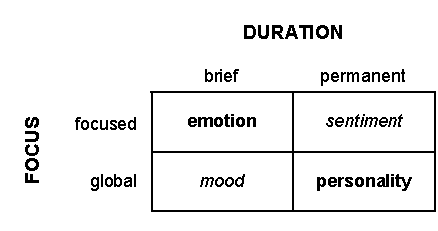
\includegraphics[width=0.45\textwidth]{figures/CR_affectTypes.pdf}

                \caption[Proposed Relation Between Emotion and Other Affective
                Types]{Proposed Relation Between Emotion and Other Affective
                Types (Adapted from \citet[p.~136]{moffat1997personality})}
                \label{fig:CRAffectTypes}
            \end{figure}

            \item Could derive core affect from emotion process via the
            \textit{valence} and \textit{demand character} appraisal
            dimensions and arousal value~\citep[p.~207,
            454]{frijda1986emotions}
        \end{itemize}

        \item Inclusion of a ``Regulation Processes" block that can affect
        nearly all parts of the emotion
        process~\citep[p.~545]{frijda1986emotions}
        \begin{itemize}
            \item Multiple points to introduce new components and processes
            $\rightarrow$ easy to add non-affective components

            \item Potential to violate \textit{Hiding the Complexity of Emotion
                Generation} (\ref{easeHide}) if users can access points directly
            $\rightarrow$ create an interface to hide entry points, make it
            easier to use and understand
        \end{itemize}
    \end{itemize}

    \item \textbf{Lazarus} (\weak)
    \begin{itemize}
        \item Personality not seen as a set of innate traits that manifest in
        appraisal and coping~\citep[p.~316]{lazarus1991emotion}, defined as a
        collection of goals, needs, commitments, knowledge, attitudes, and
        beliefs that influence how an event is perceived and how the individual
        acts on the resulting action tendency~\citep[p.~623--624,
        628]{smith1990emotion} $\rightarrow$ implicitly defined
        \begin{itemize}
            \item  Affords flexibility (i.e. not limited to a set of values)
            $\rightarrow$ supports creative freedom, definitions of individual
            characters based on their goals and knowledge rather than numerical
            values

            \item More difficult to define personality quickly (e.g. have to
            decide what beliefs a character with a desired personality would
            have)
        \end{itemize}

        \item Mood is ``an existential state or condition of life'' that is
        appraisal-dependent, related to subjective
        well-being~\citep[p.~266--267]{lazarus1991emotion}
        \begin{itemize}
            \item Could define as a state that aggregates appraisal results
            into a ``satisfaction/dissatisfaction'' value
        \end{itemize}

        \item Equates affect to subjective
        experience~\citep[p.~57]{lazarus1991emotion}
        \begin{itemize}
            \item Could define core affect using \textit{goal congruence} as
            \textit{valence}

            \item arousal is part of an action tendency, tied to the
            emotion's core relational theme~\citep[p.~58--59,
            150]{lazarus1991emotion} $\rightarrow$ not explicitly defined
        \end{itemize}

        \item Potential interface points for external processes part of input
        generation/output manipulation~\citep[p.~210]{lazarus1991emotion}
        $\rightarrow$ does not have to integrate with emotion generation
        process, trivial to add non-affective components
    \end{itemize}

    \item \textbf{Scherer} (\weak)
    \begin{itemize}
        \item Proposes definitions for mood and
        personality~\citep[p.~140--141]{scherer2000psychological}, but are not
        accounted for in the working theory~\citep[p.~93,
        119]{scherer2001appraisalB}
        \begin{itemize}
            \item Personality could be defined as sensitivities in appraisal
            dimension and register functions, mood as temporary sensitivities
            caused by previous appraisals $\rightarrow$ potential to violate
            psychological validity
        \end{itemize}

        \item No clear connection to core affect

        \item Potential to integrate non-affective components at the
        information processing, appraisal objective
        steps~\citep[p.~104]{scherer2001appraisalB} $\rightarrow$ might require
        knowledge of how those components work, violating \textit{Hiding the
            Complexity of Emotion Generation} (\ref{easeHide})
    \end{itemize}

    \item \textbf{Roseman} (\weak)
    \begin{itemize}
        \item Suggests that mood and personality are tied to emotion
        generation~\citep[p.~81--83]{roseman2001model}, ways to describe
        appraisal styles for individual or families of
        emotion~\citep[p.~88--89]{roseman2001model} $\rightarrow$ implicitly
        defined
        \begin{itemize}
            \item  Affords flexibility (i.e. not limited to a set of values)
            $\rightarrow$ supports creative freedom, definitions of individual
            characters based on their goals and knowledge rather than numerical
            values

            \item More difficult to define quickly (e.g. have to decide what
            appraisal dispositions a character with a desired personality would
            have)

            \item Could be extended to represent cultural influences on emotion
            generation
        \end{itemize}

        \item No clear connection to core affect
        \begin{itemize}
            \item Could define core affect using \textit{situational state} and
            \textit{motivational state} as \textit{valence}

            \item No obvious component for arousal
        \end{itemize}

        \item Focus on the relationship between appraisal values and
        emotions~\citep[p.~81]{roseman2001model} $\rightarrow$ does not focus
        on other parts of the generation process, no obvious place to integrate
        non-affective processes
    \end{itemize}

    \item \textbf{OCC} (\strong)
    \begin{itemize}
        \item Proposes that personality is a unique parameter profile defining
        how emotion generation behaves within and between process
        levels~\citep[p.~189--190]{ortony2005affect}
        \begin{itemize}
            \item Tuning emotion generation for each NPC $\rightarrow$
            personality implicitly supported by \textit{Customizing Existing
                CME Task Parameters} (\ref{flexCustom})

            \item Could implement personality inventories as parameter
            profiles~\citep[p.~191--192]{ortony2005affect} $\rightarrow$ no
            explicit definitions given, potential to violate psychological
            validity if done incorrectly, might not matter if the profiles do
            what the developer expects
        \end{itemize}

        \item Moods described as free-floating, object-less affective states
        that can influence emotion but can also arise from sources
        independently of emotion~\citep[p.~27]{clore2000cognition}
        $\rightarrow$ could be linked to personality ``parameter profiles'' by
        treating it as an initial condition
        \begin{itemize}
            \item Defined as temporally-driven parameter changes~\citep[p.~184,
            189--190]{occ} $\rightarrow$ implicitly supported by
            \textit{Customizing Existing CME Task Parameters} (\ref{flexCustom})
        \end{itemize}

        \item Potential to represent core affect
        \begin{itemize}
            \item Physiological arousal is a global intensity variable,
            roughly proportional to base emotion
            intensity---approximately represented by the sum of the absolute
            unsigned values of some variables\footnote{\textit{desireability},
                \textit{undesireability}, \textit{praiseworthiness},
                \textit{blameworthiness}, \textit{appealingness}, and
                \textit{unappealingness}}---or perhaps even only parts of this
            (i.e. subjective importance of the situation)~\citep[p.~51,
            65--66]{occ} $\rightarrow$ other factors can influence it, and has
            a slow rate of decay, supports \textit{Customizing Existing CME
                Task Parameters} (\ref{flexCustom})

            \item It follows that \textit{valence} might be approximated as sum
            of the absolute signed values of the same variables (i.e. is the
            overall feeling positive or negative?)
        \end{itemize}

        \item Two potential ways to integrate non-affective components
        \begin{itemize}
            \item As part of the input generation process $\rightarrow$
            designer-driven, supports \textit{Ability to Operate on Different
                Levels of NPC Complexity} (\ref{flexComplex})

            \item As a method for controlling task parameters $\rightarrow$
            implicitly supported by \textit{Customizing Existing CME Task
                Parameters} (\ref{flexCustom})
        \end{itemize}
    \end{itemize}

    \item \textbf{Smith \& Kirby} (\weak)
    \begin{itemize}
        \item No clear definitions for personality, mood, or core affect
        \begin{itemize}
            \item Potential correlation between \textit{emotion-focused coping
                potential} and some personality traits~\citep[p.~1366--1368,
            1369]{smith2009putting} $\rightarrow$ suggests that personality are
            parameters on the emotion generation process

            \item Core affect could be constructed from \textit{motivational
                congruence} (as \textit{valence}) and \textit{motivational
                relevance}
            (as arousal) $\rightarrow$ not necessarily empirically
            supported, potential to violate psychological validity
        \end{itemize}

        \item Appraisal registers synthesize information from multiple sources,
        levels of processing~\citep[p.~130]{smith2001toward}
        \begin{itemize}
            \item Multiple points to introduce new components and processes
            $\rightarrow$ easy to add non-affective components

            \item Integrating non-affective components would require
            manipulating the detector mechanisms, potential to violate
            \textit{Hiding the Complexity of Emotion Generation}
            (\ref{easeHide}) if users can access points directly $\rightarrow$
            create an interface to hide entry points, make it easier to use and
            understand
        \end{itemize}
    \end{itemize}

    \item \textbf{Oatley \& Johnson-Laird} (\strong)
    \begin{itemize}
        \item Emotions often have moods and sentiments associated with
        them~\citep[p.~87]{oatley2000sentiments} $\rightarrow$ implies that
        adding these affective types would be an extension of existing emotion
        structures

        \item Temperaments (i.e. personality traits) hypothesized to be enduring
        predispositions towards emotion ``modes''
        (\citepg{oatley1987towards}{34}; \citepg{oatley1992best}{61})
        \begin{itemize}
            \item Also defines sentiments---enduring emotional dispositions
            about something, typically other
            individuals~\citep[p.~81]{oatley2000sentiments} $\rightarrow$
            potential to define two sets of personality traits (general and
            target-specific), affords more creative freedom
        \end{itemize}

        \item Moods defined directly in the theory as control signals that
        persist after the cause of an emotion passes/no longer associated with
        semantic content and keeps the system in a particular state
        (\citepg{oatley1987towards}{32}; \citepg{oatley1992best}{64})
        \begin{itemize}
            \item Could be realized as a temporary predispositions towards
            emotion ``modes'' or a longer lasing, low intensity emotion
            state~\citep[p.~34--35]{oatley1987towards} $\rightarrow$ potential
            to allow both, give user the choice of which to use, affording more
            creative freedom
        \end{itemize}

        \item Potential to define core affect based on how a goal is affected
        (positive or negative) for \textit{valence}, emotion intensity as
        arousal $\rightarrow$ no explicit definitions given, potential to
        violate psychological validity if done incorrectly, might not matter if
        the profiles do what the developer expects

        \item Assume that the cognitive system is modular and
        asynchronous~\citep[p.~31]{oatley1987towards} $\rightarrow$ implies
        that adding non-affective processes is feasible, should not require
        knowledge of the inner workings of emotion generation
    \end{itemize}
\end{itemize}

\subsubsection{Flexibility: Choosing NPC Emotions (\ref{flexEm})}
Like the discrete theories, the appraisal theories tend to define emotions as
categories to group different aspects of a response together. In this sense,
excluding predefined emotions is trivial. Once again, \textit{adding} new ones
is unclear and there are no obvious ``rules'' to follow. \progname{} can still
take advantage of them though, because new emotions need only make sense to the
developer so that they can use them. Therefore, the appraisal theories are
evaluated for what a developer would need to do and how easy it is to realize.

\begin{itemize}
    \item \textbf{Frijda} (\weak)
    \begin{itemize}
        \item Emotions as descriptions of action readiness in response to
        different combinations of events, or by the nature of the emotional
        object~\cite[p.~72--74]{frijda1986emotions} $\rightarrow$ defining new
        emotions requires defining new action tendencies
        \begin{itemize}
            \item Require modifications to the emotion generation process (i.e.
            defining appraisal patterns) $\rightarrow$ violates \textit{Hiding
                the Complexity of Emotion Generation} (\ref{easeHide})

            \item Some ``non-basic'' emotions are blends, can define a limited
            set of additional emotions $\rightarrow$ limited flexibility

            \item Define emotions by pairing existing ones with an event or
            object type and assigning it a new name $\rightarrow$ similar to
            scripting, event-coding
        \end{itemize}
    \end{itemize}

    \item \textbf{Lazarus} (\weak)
    \begin{itemize}
        \item Emotions associated with themes that can
        coexist~\citep[p.~229]{lazarus1991emotion}
        \begin{itemize}
            \item Potential to allow developers to create named combinations
            representing ``new'' emotions $\rightarrow$ necessarily create more
            complicated emotions

            \item Defining emotions that are not combinations would require new
            appraisal pattern definitions (i.e. modify emotion generation
            process) $\rightarrow$ violates \textit{Hiding the Complexity of
                Emotion Generation} (\ref{easeHide})
        \end{itemize}
    \end{itemize}

    \item \textbf{Scherer} (\good)
    \begin{itemize}
        \item ``Emotions'' defined as the net effect of continuous,
        fluctuating subsystem changes~\citep[p.~106, 108]{scherer2001appraisalB}
        \begin{itemize}
            \item Adding new emotions requires identification and naming of a
            set of subsystem changes (i.e. requires an understanding of how
            emotions are generated) $\rightarrow$ violates \textit{Hiding the
                Complexity of Emotion Generation} (\ref{easeHide})
        \end{itemize}

        \item ``Innate'' emotions\footnote{Scherer calls them \textit{modal}
            emotions.} (e.g. \textit{Joy}) attributed to common adaptational
            issues
        that produce consistent system effects~\citep[p.~108,
        113]{scherer2001appraisalB} $\rightarrow$ range of known emotions are
        products of mixtures and/or blends of ``innate'' ones
        \begin{itemize}
            \item Some emotion profiles have ``open'' entries that can accept
            any value for that dimension $\rightarrow$ potential to define
            emotion family ``members'' by providing specific values for
            ``open'' entries, potential to violate \textit{Hiding the
                Complexity of Emotion Generation} (\ref{easeHide})

            \item Intensity differences can also differentiate otherwise
            identical emotions $\rightarrow$ define new emotions by intensity
            class, external to the emotion generation process so no violation
            of \textit{Hiding the Complexity of Emotion Generation}
            (\ref{easeHide})
        \end{itemize}
    \end{itemize}

    \item \textbf{Roseman} (\good)
    \begin{itemize}
        \item Proposes that more than one emotion can be experienced
        simultaneously due to different
        evaluations~\citep[p.~81]{roseman2001model}
        \begin{itemize}
            \item Definition of new emotions as mixtures $\rightarrow$ external
            to the generation process, so no violation of \textit{Hiding the
                Complexity of Emotion Generation} (\ref{easeHide})

            \item Emotions are logically grouped by response strategy (e.g.
            \textit{attack}, \textit{exclude}) $\rightarrow$ potential for a
            design tool to guide the process of defining new emotions?
        \end{itemize}
    \end{itemize}

    \item \textbf{OCC} (\good)
    \begin{itemize}
        \item Emotions necessarily tied to cognitive abilities that build on
        four basic affective states~\citep[p.~183--184]{ortony2005affect}
        implies that adding ``new'' emotions is about adding meaning
        $\rightarrow$ dependent on what is available for inputs,
        designer-driven, supports \textit{Ability to Operate on Different
            Levels of NPC Complexity} (\ref{flexComplex})

        \item Propose smaller emotion structure for believable agents,
        collapsing 22 emotions into five positive and five negative
        ones~\citep[p.~193--194]{ortony2002making}
        \begin{itemize}
            \item Potential to add ``new'' emotions as more cognitive processes
            are added $\rightarrow$ dependent on what is available for inputs,
            designer-driven, supports \textit{Ability to Operate on Different
                Levels of NPC Complexity} (\ref{flexComplex})
        \end{itemize}

        \item \textit{Surprise} as a special case, can be added in connection
        with the \textit{unexpectedness} appraisal variable~\citep[p.~13--14,
        16--17]{ortony2021all}

        \item ``New'' emotions can be defined as differences in
        intensity/elicitation thresholds (e.g. \textit{Pleased} for low
        intensity and \textit{Ecstatic} for high)~\citep[p.~185]{occ}
        \begin{itemize}
            \item External to the emotion generation process $\rightarrow$ no
            violation of \textit{Hiding the Complexity of Emotion Generation}
            (\ref{easeHide})
        \end{itemize}
    \end{itemize}

    \item \textbf{Smith \& Kirby} (\weak)
    \begin{itemize}
        \item Unclear how additional emotions could be defined

        \item Hypothesizes that emotion categories are likely dense clusters in
        dimensional space~\citep[p.~245--246]{smith_scott_mandler_1997}
        \begin{itemize}
            \item Potential to combine with V-A or PAD Space, define new
            emotion categories from existing data clusters $\rightarrow$ would
            require some understanding of source material, potential violation
            of \textit{Hiding the Complexity of Emotion Generation}
            (\ref{easeHide})

            \item Developers could collect their own data to find affective
            ``clusters'' in a dimensional space $\rightarrow$ time consuming,
            error-prone, potential violation of \textit{Hiding the Complexity
                of Emotion Generation} (\ref{easeHide})
        \end{itemize}
    \end{itemize}

    \item \textbf{Oatley \& Johnson-Laird} (\strong)
    \begin{itemize}
        \item How people describe emotions in everyday language indicates
        underlying cognitive meanings~\citep[p.~210]{johnson1992basic}
        $\rightarrow$ can build on layperson's understanding of emotions,
        supports \textit{Hiding the Complexity of Emotion Generation}
        (\ref{easeHide})

        \item Emotion ``modes'' are not absolute definitions, only have
        heuristic properties that capture general classes of
        events~\citep[p.~87]{oatley2000sentiments} $\rightarrow$ potential to
        create more refined emotions by constraining the classes
        \begin{itemize}
            \item ``New''/''adult'' emotions are based on emotion ``modes'',
            deliberative processes attach more meaning to them
            (\citepg{oatley1987towards}{35, 43};
            \citepg{oatley1992best}{76--78})

            \item Can also be defined at junctions of mutual plans with one or
            more other agents, requires a self-model~\citep[p.~44, 46,
            48]{oatley1987towards} $\rightarrow$ way to integrate cultural
            differences due to the impact on models and reasoning
            processes~\citep[p.~47]{oatley1987towards}
        \end{itemize}

        \item Emotions that have different semantic contents can exist
        simultaneously~\citep[p.~104]{oatley1992best} $\rightarrow$ potential
        to define emotion ``mixtures''
        \begin{itemize}
            \item External to the emotion generation process $\rightarrow$ no
            violation of \textit{Hiding the Complexity of Emotion Generation}
            (\ref{easeHide})
        \end{itemize}
    \end{itemize}
\end{itemize}

\subsubsection{Flexibility: Allowing Developers to Specify How to Use CME
Outputs
    (\ref{flexOut})}
There is clearly a difference between reflexes and emotions: one is very
difficult to control how one reacts and the other has a range of them to pick
from~\citep[p.~45]{fellous2004human}. The idea of emotion \textit{components}
also suggests that there is flexibility in which system aspects are affected
and how (\citepg{hudlicka2019modeling}{133};
\citepg{scherer2001appraisalB}{108}; \citepg{roseman2011emotional}{436}). This
implies that \textit{any} appraisal theory should be able to strongly support
this requirement. The question is now how well each theory defines what this
means.

\begin{itemize}
    \item \textbf{Frijda} (\strong)
    \begin{itemize}
        \item Set the output boundary of \progname{} at the action proposer
        (i.e. action tendency), relevance and control precedence signals, and
        physiological change generators (i.e. arousal)
        points~\citep[p.~455]{frijda1986emotions}
        \begin{itemize}
            \item Would also allow for another layer to group these into
            emotion categories~\citep[p.~72]{frijda1986emotions}

            \item Can feed the outputs back into \progname{} $\rightarrow$
            provide an interface so that this is a matter of ``flipping a
            switch'', supported by \textit{Customizing Existing CME Task
                Parameters} (\ref{flexCustom})

            \item [$\rightarrow$] Allows maximum flexibility for defining what
            to do with outputs that is agnostic to how ``action'' is defined
        \end{itemize}
    \end{itemize}

    \item \textbf{Lazarus} (\strong)
    \begin{itemize}
        \item Set the output boundary of \progname{} at the appraisal outcome
        (i.e. action tendency, subjective experience, physiological response),
        would also allow for labelling the output with emotion
        categories~\citep[p.~209--210]{lazarus1991emotion}
        \begin{itemize}
            \item Excludes coping process integral to the theory $\rightarrow$
            could be added as an external component, supported by
            \textit{Allowing the Integration of New CME Components}
            (\ref{flexNew})

            \item Resulting NPC actions would impact their interpretation of
            the environment $\rightarrow$ implicitly supports reappraisal
            process~\citep[p.~134]{lazarus1991emotion}

            \item Can feed the outputs back into \progname{} $\rightarrow$
            provide an interface so that this is a matter of ``flipping a
            switch'', supported by \textit{Customizing Existing CME Task
                Parameters} (\ref{flexCustom})

            \item [$\rightarrow$] Allows maximum flexibility for defining what
            to do with outputs that is agnostic to how ``action'' is defined
        \end{itemize}
    \end{itemize}

    \item \textbf{Scherer} (\strong)
    \begin{itemize}
        \item Set the output boundary of \progname{} at the action tendency
        level, would also allow for labelling the output with emotion
        categories~\citep[p.~107, 113]{scherer2001appraisalB} $\rightarrow$
        allows maximum flexibility for defining what to do with outputs that is
        agnostic to how ``action'' is defined

        \item Allow users to access individual appraisal
        registers~\citep[p.~104]{scherer2001appraisalB} $\rightarrow$ affords
        more flexibility
        \begin{itemize}
            \item Each part of the appraisal process makes changes to different
            subsystems, creates a continuously changing
            outputs~\citep[p.~107]{scherer2001appraisalB} $\rightarrow$
            appraisal ``history" encoded in unique pattern caused by subsystem
            changes, values update frequently

            \item Potential to violate \textit{Hiding the Complexity of Emotion
                Generation} (\ref{easeHide}) $\rightarrow$ make available for
            advanced users

            \item Potential to violate psychological validity $\rightarrow$ how
            a user uses the values should be external to \progname{}, so its
            internal psychological validity would remain intact
        \end{itemize}
    \end{itemize}

    \item \textbf{Roseman} (\strong)
    \begin{itemize}
        \item Set the output boundary of \progname{} at the ``response
        strategy'', the typical physiological, phenomenological, expressive,
        behavioural, and motivational emotion contents
        (\citepg{roseman2013appraisal}{141}; \citepg{roseman2001model}{75};
        \citepg{roseman2018functions}{146--148, 151--152})
        \begin{itemize}
            \item Potential to connect components directly to existing game
            modules if available (e.g. ``expressive'' as an input to NPC
            animation, ``motivation'' to planning) $\rightarrow$ user chooses
            which ones to use, supported by \textit{Choosing Which CME Tasks to
                Use} (\ref{flexTasks})

            \item Differentiates between ``action tendency'' and what action is
            actually taken, informed by emotion
            intensity~\citep[p.~436]{roseman2011emotional} $\rightarrow$ input
            to the behaviour/expression selection process, explicitly built-in
            support for \textit{Allowing Developers to Specify How to Use CME
                Outputs} (\ref{flexOut})

            \item Also notes that there is consistency in what types of
            responses that each emotion elicits~\citep{roseman2011emotional}
            $\rightarrow$ creates consistent behaviour necessary for
            believability~\citep[p.~200]{ortony2002making}

            \item [$\rightarrow$] Allows maximum flexibility for defining what
            to do with outputs that is agnostic to the system at large
        \end{itemize}
    \end{itemize}

    \item \textbf{OCC} (\strong)
    \begin{itemize}
        \item Set the output boundary of \progname{} at the evaluation of
        emotion category and intensity~\citep[p.~19, 69]{occ}
        \begin{itemize}
            \item Propose that action tendencies are not necessary or
            sufficient to define emotion because some emotions might not have a
            ``characteristic" action tendency as defined as voluntary actions
            following emotion~\citep[p.~11]{occ} $\rightarrow$ allows the
            generation of emotions that do not have one, removes constraint
            from user

            \item Claims ``action tendency'' is a set of components that
            emotions constrain themselves to, but might not use all
            components~\citep[p.~198, 201]{ortony2002making} $\rightarrow$
            creates consistent behaviour necessary for
            believability~\citep[p.~200]{ortony2002making}

            \item [$\rightarrow$] Allows maximum flexibility for defining what
            to do with outputs that is agnostic to the system at large
        \end{itemize}
    \end{itemize}

    \item \textbf{Smith \& Kirby} (\strong)
    \begin{itemize}
        \item Set the output boundary of \progname{} at ``emotional response'',
        contains appraisal outcome (e.g. emotion category and dimensions,
        intensity), physiological activity (e.g. arousal, facial
        expressions), and action tendencies~\citep[p.~123, 130]{smith2001toward}
        \begin{itemize}
            \item Users can separate components and send them to different
            system process

            \item Can also send components back into appraisal processes via
            appraisal sources $\rightarrow$ potential for different
            interpretations due to processing in appraisal
            source~\citep[p.~99]{smith2000consequences}

            \item [$\rightarrow$] Allows maximum flexibility for defining what
            to do with outputs that is agnostic to the system at large
        \end{itemize}
    \end{itemize}

    \item \textbf{Oatley \& Johnson-Laird} (\strong)
    \begin{itemize}
        \item Set the output boundary of \progname{} at control signals,
        labelled with an emotion category~\citep[p.~50, 54]{oatley1992best}

        \item Control signals are global entities or ``alarms'' that change the
        system ``mode'' when a goal is impacted by an active plan, bringing it
        into focus~\citep[p.~62--63]{oatley1992best}
        \begin{itemize}
            \item Users can choose which system components are receptive to the
            signal and to what degree $\rightarrow$ supported by
            \textit{Choosing Which CME Tasks to Use} (\ref{flexTasks}) and
            \textit{Customizing Existing CME Task Parameters} (\ref{flexCustom})

            \item [$\rightarrow$] Allows maximum flexibility for defining what
            to do with outputs that is agnostic to the system at large
        \end{itemize}
    \end{itemize}
\end{itemize}

\subsubsection{Flexibility: Ability to Operate on Different Levels of NPC
    Complexity (\ref{flexComplex})}
Due to the assumed role of cognition in emotion processes
(\citepg{marsella2015appraisal}{55}; \citepg{broekens2021emotion}{354}), there
is also an assumed level of NPC complexity needed for an appraisal-based CME to
properly function. Therefore, the appraisal theories are evaluated based on how
much cognitive processing is required to produce results.

\begin{itemize}
    \item \textbf{Frijda} (\weak)
    \begin{itemize}
        \item Requires encoded categories for events and rules for inputs,
        action structures for evaluating coping, process to evaluate
        event/action implications, definition of concern
        structures~\citep[p.~457]{frijda1986emotions} $\rightarrow$ effort to
        create likely to linearly increase with respect to game complexity
        \begin{itemize}
            \item Some can be implicitly evaluated in \progname{} $\rightarrow$
            relieves some of the authorial burden from game designers
        \end{itemize}

        \item Regulation processes can be added as needed, not mandated in the
        core emotion process~\citep[p.~454, 456]{frijda1986emotions}
        $\rightarrow$ can potentially adapt to increases in NPC/game complexity
        \begin{itemize}
            \item Path in process to add planning if needed, but not critical to
            function~\citep[p.~462]{frijda1986emotions}
        \end{itemize}

        \item Requires a monitoring process (i.e. blackboard structure) to
        continuously update situational
        meaning~\citep[p.~459]{frijda1986emotions} $\rightarrow$ space
        requirements increases with information sources

    \end{itemize}

    \item \textbf{Lazarus} (\strong)
    \begin{itemize}
        \item Purpose of appraisal is to ``integrate the two [personal
        interests with environmental realities] as effectively as
        possible''~\citep[p.~135]{lazarus1991emotion} $\rightarrow$ complexity
        controlled by \progname{}, can be made relatively simple

        \item Complexity in individual factors and environmental conditions
        evaluations that get passed to
        appraisal~\citep[p.~209--210]{lazarus1991emotion} $\rightarrow$
        designer controlled, can define to match game complexity
        \begin{itemize}
            \item Minimally requires definitions for goals, ``ego type", event
            causes, predictions about the impact of actions and future
            events~\citep[p.~149--150]{lazarus1991emotion}

            \item [$\rightarrow$] Could connect to hard-coded data/processes
            for low-complexity games (e.g. \textit{Pac-Man}~\citep{pacman}),
            increase complexity with game
        \end{itemize}

        \item Implication of a central data structure to store appraisal values
        as they become available~\citep[p.~134, 151, 189,
        210--211]{lazarus1991emotion}
        \begin{itemize}
            \item Stores outputs of appraisal evaluations, not the inputs

            \item [$\rightarrow$] Complexity likely to be constant or linearly
            increase with respect to the number and complexity of inputs
        \end{itemize}
    \end{itemize}

    \item \textbf{Scherer} (\strong)
    \begin{itemize}
        \item Built-in support for variable NPC complexity
        \begin{itemize}
            \item Appraisal dimension groupings (SECs) can be as complex as the
            information processing system allows, often a continuous or graded
            scalar or multidimensional
            evaluation~\citep[p.~94]{scherer2001appraisalB} $\rightarrow$
            numerical values easier to manipulate

            \item Assumes three levels of processing (sensory-motor, schematic,
            conceptual) that
            interact~\citep[p.~102--103]{scherer2001appraisalB} $\rightarrow$
            potential to derive some information in \progname{} implicitly from
            inputs
            \begin{itemize}
                \item Provide option to turn these tasks off or configure them
                $\rightarrow$ support for \textit{Choosing Which CME Tasks to
                    Use} (\ref{flexTasks}) and \textit{Customizing Existing
                    Task
                    Parameters} (\ref{flexCustom})
            \end{itemize}
        \end{itemize}

        \item Reappraisals run until a monitoring system signals termination or
        adjustment, appraisal components updated by
        reappraisals~\citep[p.~99]{scherer2001appraisalB} $\rightarrow$ game
        designer can decide when to terminate appraisal cycles based on game
        needs, support of \textit{Customizing Existing Task Parameters}
        (\ref{flexCustom}) and \textit{Be Efficient and Scalable}
        (\ref{flexScale})

        \item Appraisal registers updated as new information becomes available,
        central structure, can control relative importance of each
        value using a weighted function to represent ``goodness'' of
        data~\citep[p.~105]{scherer2001appraisalB};
        \begin{itemize}
            \item Implies a temporal and confidence value for each
            register~\citep[p.~106]{scherer2001appraisalB} $\rightarrow$ game
            designer can decide when to evaluate emotion state based on these
            values, support of \textit{Customizing Existing Task Parameters}
            (\ref{flexCustom})
        \end{itemize}
    \end{itemize}

    \item \textbf{Roseman} (\good)
    \begin{itemize}
        \item Suggestion that there are different versions of appraisal
        mechanisms of variable complexity triggered as time
        allows~\citep[p.~77]{roseman2001model}, and influenced by emotion
        intensity~\citep[p.~440]{roseman2011emotional}
        \begin{itemize}
            \item Can specify different appraisal mechanisms $\rightarrow$ game
            designers can build on top of input API, choose how information is
            synthesised into \progname{} inputs
        \end{itemize}

        \item Still requires empirical data to determine the minimum cognitive
        requirements for appraisals~\citep[p.~87--88]{roseman2001model}
        \begin{itemize}
            \item Lowest level involves fixed action
            patterns~\citep[p.~32]{clore2000cognition} $\rightarrow$
            correspondence with core \progname{} tasks, direct match between
            generated emotion and assigned behaviours for it as assigned by
            game designer

            \item With no defined process, do not know how to integrate
            cognitive processes into \progname{}
        \end{itemize}
    \end{itemize}

    \item \textbf{OCC} (\good)
    \begin{itemize}
        \item Has three levels of processing (reactive, routine,
        reflective)~\citep[p.~175--177, 179]{ortony2005affect}
        \begin{itemize}
            \item OCC proper part of the highest processing level,
            ``reflective'', does not interact with external environment
            $\rightarrow$ requires cognitive/high-level
            processes, inputs from other two levels

            \item Number of potential emotions restricted in reactive (no
            emotions) and routine (four emotions) levels $\rightarrow$ violates
            \textit{Choosing NPC Emotions} (\ref{flexEm})

            \item Assumptions make it unlikely to be applicable to
            architectures that are simpler than adult
            humans~\citep[p.~220]{sloman2005architectural}
        \end{itemize}

        \item Produce a simpler, less rigorous architecture with one processing
        level
        \begin{itemize}
            \item Complexity might lie in how variables are evaluated and how
            goals/standards/attitudes are represented, coding of rules appears
            relatively simple~\citep[p.~182--188]{occ}

            \item Could allow for user-defined evaluations and representations
            $\rightarrow$ support as a Domain-Specific Language (DSL) to avoid
            violating \textit{Hiding the Complexity of Emotion Generation}
            (\ref{easeHide})
        \end{itemize}
    \end{itemize}

    \item \textbf{Smith \& Kirby} (\strong)
    \begin{itemize}
        \item Potential to design multiple appraisal mechanisms that rely
        on different functions (e.g. planning, expectation evaluation)
        $\rightarrow$ clear distinction between available functions and
        \progname{}'s abilities
        \begin{itemize}
            \item Number of appraisal variables determines types of emotion
            available~\citep{yih2016distinct, yih2016patterns},
            \citep[p.~488--492]{yih2020profiles}

            \item [$\rightarrow$] Number of potential emotion categories tied
            to NPC complexity

            \item Potential to violate \textit{Choosing NPC Emotions}
            (\ref{flexEm}) $\rightarrow$ assuming that NPC complexity and what
            emotions the game designer wants them to have are directly
            proportional, this is unlikely to be a concern
        \end{itemize}
    \end{itemize}

    \item \textbf{Oatley \& Johnson-Laird} (\good)
    \begin{itemize}
        \item Distinguishing emotion types changes based on cognitive
        abilities~\citep[p.~40--41]{oatley1987towards}, possible goal and plan
        representations~\citep[p.~57--58]{oatley1992best}
        \begin{itemize}
            \item Emotion ``modes'' as ``base classes'' of emotion

            \item [$\rightarrow$] Number of potential emotion categories tied
            to NPC complexity

            \item Potential to violate \textit{Choosing NPC Emotions}
            (\ref{flexEm}) $\rightarrow$ assuming that NPC complexity and what
            emotions the game designer wants them to have are directly
            proportional, this is unlikely to be a concern
        \end{itemize}
    \end{itemize}
\end{itemize}

\subsubsection{Flexibility: Be Efficient and Scalable (\ref{flexScale})}
The main concern for the efficiency and scalability of the appraisal theories
is how they evaluate inputs. However, this complexity seems to lie in creating
the inputs. Since this precedes their transformation into emotions, action
tendencies, and other components, a lot of this burden is passed to the game
developer. Ideally, \progname{} would handle more of these tasks. However, this
also allows developers to choose how they want to generate inputs. Ultimately
this gives them more freedom, and allows \progname{} to merge more easily into
different games and underlying architectures. What \progname{} focuses on,
then, is helping game developers manage different evaluation processes.

\begin{itemize}
    \item \textbf{Frijda} (\good)
    \begin{itemize}
        \item Uses 17--24 appraisal dimensions to create unique profiles for
        emotions, not all dimensions needed for each emotion
        (\citepg{frijda1986emotions}{205--219};
        \citepg{frijda1987emotion}{121--124})
        \begin{itemize}
            \item Efficiency might be hindered if more dimensions are evaluated
            than are needed

            \item Give developers choice of appraisal dimensions $\rightarrow$
            compromises \textit{Hiding the Complexity of Emotion Generation}
            (\ref{easeHide})
        \end{itemize}

        \item Scalability mostly driven by complexity of inputs and
        externally-defined regulation processes $\rightarrow$ depends on
        complexity of evaluations to generate inputs, designer-driven
    \end{itemize}

    \item \textbf{Lazarus} (\strong)
    \begin{itemize}
        \item Dependent on knowledge~\citep[p.~145]{lazarus1991emotion},
        knowledge evaluation mechanisms $\rightarrow$ depends on designer chosen
        architecture

        \item Appraisal process appears to be of a fixed complexity once inputs
        are given~\citep[p.~210]{lazarus1991emotion}, implies that scalability
        depends on complexity of knowledge processes and inputs $\rightarrow$
        depends on complexity of evaluations to generate inputs, designer-driven
    \end{itemize}

    \item \textbf{Scherer} (\good)
    \begin{itemize}
        \item Uses 16 appraisal dimensions divided into four
        groups~\citep[p.~114--115]{scherer2001appraisalB} $\rightarrow$ minimum
        set of appraisal dimensions necessary to differentiate emotion
        families~\citep[p.~94]{scherer2001appraisalB}

        \item Groups are evaluated in order to avoid using unneeded expensive
        processes~\citep[p.~99--100, 102--103]{scherer2001appraisalB}
        \begin{itemize}
            \item Does not exclude potential to begin getting partial results by
            running the four components in parallel

            \item Groups can have more than one associated process
            $\rightarrow$ lower level processes for each group first, higher
            level processes only used if they do not return results

            \item Can add a central controller to allow integration of
            additional processes similar to Smith \& Kirby appraisal
            detector~\citep[p.~103--105]{scherer2001appraisalB}

            \item [$\rightarrow$] Efficiency tied to the complexity of inputs,
            partially designer-driven

            \item [$\rightarrow$] Mechanisms for scalability built-in, but
            requires more overhead costs to manage them, might conflict with
            \textit{Ability to Operate on Different Levels of NPC Complexity}
            (\ref{flexComplex})
        \end{itemize}
    \end{itemize}

    \item \textbf{Roseman} (\weak)
    \begin{itemize}
        \item Suggests that there are different versions of appraisal
        mechanisms of variable complexity triggered as time
        allows~\citep[p.~77]{roseman2001model} $\rightarrow$ potential for
        scalability, efficiency

        \item Focuses on the structure of emotions and appraisal
        dimensions~\citep[p.~68, 81]{roseman2001model} $\rightarrow$ no further
        information given
    \end{itemize}

    \item \textbf{OCC} (\good)
    \begin{itemize}
        \item Uses 3--19 variables to differentiate emotion families, not all
        variables needed for each emotion~\citep[p.~19, 60, 69]{occ}
        $\rightarrow$ can prevent evaluation of some variables based on which
        branch of the tree is active

        \item Efficiency tied to complexity of inputs~\citep[p.~182--188]{occ}
        $\rightarrow$ tied to evaluation mechanisms, designer-driven

        \item Can introduce mechanisms such that lower-complexity processes run
        first and call higher-complexity processes if they cannot produce a
        result~\citep[p.~179]{ortony2005affect} $\rightarrow$ more control of
        efficiency and scalability

        \item Can have two parallel emotion-elicitation mechanisms
        $\rightarrow$ can produce conflicting results~\citep[p.~37--39,
        54]{clore2000cognition}
        \begin{itemize}
            \item Memory-based heuristics, which is faster and more error-prone
            $\rightarrow$ improved efficiency, could run into memory-related
            scalability issues

            \item Deliberative processing, which is slower and less error-prone
            $\rightarrow$ reduced efficiency, more scale-friendly

            \item [$\rightarrow$] Could create a more believable result, but
            might conflict with \textit{Ability to Operate on Different Levels
                of NPC Complexity} (\ref{flexComplex})
        \end{itemize}
    \end{itemize}

    \item \textbf{Smith \& Kirby} (\strong)
    \begin{itemize}
        \item Uses 7--16 variables to create unique profiles for emotions, not
        all dimensions needed for each emotion (\citepg{yih2020profiles}{489};
        \citeg{yih2016distinct})
        \begin{itemize}
            \item Efficiency might be hindered if more dimensions are evaluated
            than are needed

            \item Give developers choice of appraisal dimensions $\rightarrow$
            compromises \textit{Hiding the Complexity of Emotion Generation}
            (\ref{easeHide})
        \end{itemize}

        \item A few variables could be evaluated by \progname{} (e.g.
        \textit{motivational relevance}) $\rightarrow$ efficiency and
        scalability controlled by \progname{}

        \item Some evaluation processes produce inputs \textit{for} \progname{}
        $\rightarrow$ designer-driven, architecture dependent
        \begin{itemize}
            \item Appraisal detector continuously monitors for changes in
            variables, combines information and called appraisal
            process~\citep[p.~129--130]{smith2001toward} $\rightarrow$
            implicitly enforces scalability as developers add and remove
            processes
            \begin{itemize}
                \item Detector must only require minimal resources to function
                well~\citep[p.~90--91]{smith2000consequences} $\rightarrow$
                acknowledges that efficiency is essential
            \end{itemize}

            \item Support for multiple, parallel user-defined processes that
            could have variable complexity
            levels~\citep[p.~91--92]{smith2000consequences} $\rightarrow$
            create mechanism for developers to define when complex processes
            activate
        \end{itemize}
    \end{itemize}

    \item \textbf{Oatley \& Johnson-Laird} (\strong)
    \begin{itemize}
        \item Assumes a system that coordinates multiple plans and goals under
        time and resource constraints (e.g. plans only work 1--2 steps
        ahead)~\citep[p.~31, 36]{oatley1987towards} $\rightarrow$ property of
        the architecture, designer-driven

        \item Goals and plans associated with emotion has their own monitoring
        mechanisms~\citep[p.~50]{oatley1992best} $\rightarrow$ can decide which
        ones to associate with \progname{}, built in scalability
        \begin{itemize}
            \item Mechanism would work on goal and plan information
            $\rightarrow$ can be made efficient
        \end{itemize}

        \item Emotions can be given more complex meanings by evaluating more
        information via selective function
        calls~\citep[p.~32--34]{oatley1987towards} $\rightarrow$
        designer-dependent and ties scalability, efficiency to the needs of the
        game, supports \textit{Ability to Operate on Different Levels of NPC
            Complexity} (\ref{flexComplex})
    \end{itemize}
\end{itemize}

\subsubsection{Ease-of-Use: Hiding the Complexity of Emotion Generation
    (\ref{easeHide})}
The appraisal theories generally have strong support for this requirement.
Designers do not need to known what is done with the inputs they provide, so
the processing of those inputs can be hidden from them.

\begin{itemize}
    \item \textbf{Frijda} (\strong)
    \begin{itemize}
        \item System arranged so that information can be supplied at any point
        to black box processes, tracked by an internal monitor/situational
        meaning blackboard structure~\citep[p.~455--456,
        459]{frijda1986emotions} $\rightarrow$ do not need to know how the
        process uses information
    \end{itemize}

    \item \textbf{Lazarus} (\strong)
    \begin{itemize}
        \item Appraisal assigns personal meaning to
        knowledge~\citep[p.~145]{lazarus1991emotion} $\rightarrow$ do not need
        to know how the process uses information

        \item Six appraisal dimensions, reappraisal accounts for changes to
        input values~\citep[p.~134, 149--150]{lazarus1991emotion} $\rightarrow$
        can incorporate changing information as a queue of input values
    \end{itemize}

    \item \textbf{Scherer} (\strong)
    \begin{itemize}
        \item Inputs combined into
        registers~\citep[p.~105]{scherer2001appraisalB}, patterns of register
        values matched to emotions~\citep[p.~114--115]{scherer2001appraisalB}
        $\rightarrow$ do not need to know how this is done
        \begin{itemize}
            \item Some dimensions are pure information (e.g. \textit{intrinsic
                pleasantness})~\citep[p.~146]{lazarus1991emotion} $\rightarrow$
            inherently hides process complexity

            \item Appraisal dimension groupings (SECs) can be divided into
            hard-wired and deliberative
            units~\citep[p.~102]{scherer2001appraisalB} $\rightarrow$ do not
            need to know which ones are deliberative or not
        \end{itemize}

        \item Changes in SECs can cause continuously changing
        outputs~\citep[p.~107]{scherer2001appraisalB} $\rightarrow$ need only
        query if there has been a change, do not need to know if the generation
        process triggered
    \end{itemize}

    \item \textbf{Roseman} (\good)
    \begin{itemize}
        \item Inputs pattern-matched to emotion families~\citep[p.~70--71,
        81]{roseman2001model} $\rightarrow$ do not need to know what the
        patterns are

        \item Focus on the relationship between appraisal values and
        emotions~\citep[p.~81]{roseman2001model} $\rightarrow$ does not focus
        on other parts of the generation process
    \end{itemize}

    \item \textbf{OCC} (\good)
    \begin{itemize}
        \item Inputs pattern-matched to emotions, combined into intensity
        values, and compared to threshold rules~\citep[p.~69, 189]{occ}
        $\rightarrow$ do not need to know how this is done

        \item Need to know patterns of variables to support \textit{Choosing
            NPC Emotions} (\ref{flexEm}) $\rightarrow$ potential to expose
            variable
        patterns, but not how the variables are combined or compared to
        threshold rules
    \end{itemize}

    \item \textbf{Smith \& Kirby} (\good)
    \begin{itemize}
        \item Inputs combined into single unit by appraisal
        register, triggers generation process~\citep[p.~130]{smith2001toward}
        $\rightarrow$ do not need to know how this is done

        \item Need to know patterns of variables to support \textit{Choosing
            NPC Emotions} (\ref{flexEm}) (\citepg{yih2020profiles}{489};
        \citeg{yih2016distinct}) $\rightarrow$ potential to expose variable
        patterns, but not how they are used
    \end{itemize}

    \item \textbf{Oatley \& Johnson-Laird} (\good)
    \begin{itemize}
        \item Emotions as products of interpretations of goals and
        plans~\citep[p.~30]{oatley1987towards} $\rightarrow$ do not need to
        know how they are interpreted

        \item Need to provide additional information to support
        \textit{Choosing NPC Emotions} (\ref{flexEm})
        \begin{itemize}
            \item Add contextual information to generated
            emotion~\citep[p.~76--78]{oatley1992best} $\rightarrow$ does not
            require knowledge of how the emotion was produced

            \item Tied to ``folk'' understanding of emotions, their
            consequences, and antecedents~\citep[p.~214--215]{johnson1992basic}
            $\rightarrow$ minimizes potential to violate this requirement
        \end{itemize}
    \end{itemize}
\end{itemize}

\subsubsection{Ease-of-Use: Having a Clear API (Input) (\ref{easeAPI})}
It is not enough for an appraisal theory to be clear in what it requires for
appraisal. It must also be clear in what it does with those inputs to produce
an unambiguous output. Therefore, the theories are analysed for both their
necessary inputs, how those could be realized as an input interface, and how
those inputs map to appraisal outputs.

\begin{itemize}
    \item \textbf{Frijda} (\good)
    \begin{itemize}
        \item Minimally requires definition of concerns (which include goal
        definitions), environment states/events, action (tendency)
        structures~\citep[p.~454, 457]{frijda1986emotions} $\rightarrow$
        generally do not know how to define
        inputs~\citep[p.~86--87]{roseman2001model}

        \item At least 20 variables
        listed~\citep[p.~205--216]{frijda1986emotions}, smaller list of 14
        variables have preliminary empirical
        validation~\citep[p.~128--131]{frijda1987emotion} $\rightarrow$
        potential to overwhelm users with the full list
        \begin{itemize}
            \item Some variables describe knowledge (e.g.
            \textit{valence}~\citep[p.~207]{frijda1986emotions}) $\rightarrow$
            cannot be removed from input variable list

            \item Some variables could be derived from knowledge (e.g.
            \textit{change} derived from previous and current state, implicit
            in definition of ``event''~\citep[p.~209--210]{frijda1986emotions})
            $\rightarrow$ exchange variables for knowledge in input list
            \begin{itemize}
                \item Might be able to reduce the required input list if there
                are overlaps in required knowledge for many variables

                \item Replace variable names with knowledge that is generally
                understood (e.g. states, goals) $\rightarrow$ supports
                \textit{Hiding the Complexity of Emotion Generation}
                (\ref{easeHide})
            \end{itemize}

            \item Some variables might be encoded implicitly in others (e.g.
            \textit{presence/absence}, \textit{urgency}~\citep[p.~208--209,
            455]{frijda1986emotions}) $\rightarrow$ do not have to be exposed
            to user, reduce required input list in API

            \item Unique profiles for some
            emotions~\citep[p.~217--219]{frijda1986emotions}, empirical
            validation of some patterns~\citep[p.~122--123]{frijda1987emotion}
            showing that each emotion uses a subset of variables $\rightarrow$
            might be able to define subsets of variables if some emotions are
            not needed

            \item [$\rightarrow$] Options error-prone, require careful design
            of \progname{}

            \item Do not know how to define some of these
            inputs~\citep[p.~86--87]{roseman2001model}
        \end{itemize}
    \end{itemize}

    \item \textbf{Lazarus} (\disqualified)
    \begin{itemize}
        \item Minimally requires local and global ``ego-identity'' goals,
        causal agents and their control over an event, coping potential,
        predictions about future prospects~\citep[p.~102,
        149--150]{lazarus1991emotion} $\rightarrow$ generally do not know how
        to define inputs~\citep[p.~86--87]{roseman2001model}
        \begin{itemize}
            \item Correlate with five appraisal dimensions

            \item Written in natural/familiar language, conceptualized as
            entities and values $\rightarrow$ supports \textit{Hiding the
                Complexity of Emotion Generation} (\ref{easeHide})
        \end{itemize}

        \item Appraisal patterns are not clearly unique (e.g. \textit{Anxiety}
        and \textit{Disgust} only differ in ego-involvement, but what is the
        difference between ``protection against existential threats'' and
        ``being at risk of a poisonous idea''?~\citep[p.~237,
        261]{lazarus1991emotion}) $\rightarrow$ prone to assumption biases,
        threatening psychological validity
    \end{itemize}

    \item \textbf{Scherer} (\good)
    \begin{itemize}
        \item Minimally requires goals, events and their properties (e.g.
        \textit{predictability}, \textit{intrinsic pleasantness}), causality,
        predictions about events, time constraints on goals, predictions about
        the controllability over potential outcomes, ability to influence
        and/or adapt to potential outcomes, and information about the agent's
        conception of self-ideal and social norms

        \item 15 appraisal variables divided into four groups internally for
        organization and flow~\citep[p.~94]{scherer2001appraisalB}
        $\rightarrow$ potential to overwhelm users with the full list
        \begin{itemize}
            \item Some variables describe knowledge (e.g. \textit{intrinsic
                pleasantness}~\citep[p.~95]{scherer2001appraisalB})
                $\rightarrow$
            cannot be removed from input variable list

            \item Some variables could be derived from knowledge (e.g.
            \textit{discrepancy from expectation} derived from current state
            prediction about current state from previous
            ones~\citep[p.~96]{scherer2001appraisalB}) $\rightarrow$ exchange
            variables for knowledge in input list
            \begin{itemize}
                \item Might be able to reduce the required input list if there
                are overlaps in required knowledge for many variables

                \item Replace variable names with knowledge that is generally
                understood (e.g. probabilities, goals) $\rightarrow$ supports
                \textit{Hiding the Complexity of Emotion Generation}
                (\ref{easeHide})
            \end{itemize}

            \item Unique profiles for some emotions that have some empirical
            support~\citep[p.~114--117]{scherer2001appraisalB} showing that
            each emotion uses a subset of variables $\rightarrow$ might be able
            to define subsets of variables if some emotions are not needed

            \item [$\rightarrow$] Options error-prone, require careful design
            of \progname{}

            \item Do not know how to define some of these
            inputs~\citep[p.~86--87]{roseman2001model}
        \end{itemize}
    \end{itemize}

    \item \textbf{Roseman} (\good)
    \begin{itemize}
        \item Minimally requires goals, current environment states, causal
        agents, predictions and confidence values about future events, coping
        potential, if a problem is intrinsic or instrumental

        \item Seven appraisal variables create 17 emotion
        categories, accounts for all variable
        combinations~\citep[p.~68--69]{roseman2001model} $\rightarrow$
        empirically validated and compared with dimensions from other appraisal
        theories~\citep[p.~256, 260,267]{roseman1996appraisal}, revised as new
        data is collected~\citep[p.~72, 75]{roseman2001model}

        \item Generally do not know how to define these
        inputs~\citep[p.~86--87]{roseman2001model} $\rightarrow$ hypothesize
        that appraisal variables influence each other, some might be inputs to
        the evaluations of others~\citep[p.~271]{roseman1996appraisal}
    \end{itemize}

    \item \textbf{OCC} (\weak)
    \begin{itemize}
        \item Clear distinctions between events, agents, and
        objects~\citep[p.~58]{occ} $\rightarrow$ minimally requires goals,
        changes to goals, agents, standards, and preferences

        \item At least four global variables and 15 local variables to
        distinguish between emotions~\citep[p.~69]{occ} $\rightarrow$ potential
        to overwhelm users with the full list
        \begin{itemize}
            \item Reduce the list by using some variables to calculate others
            (e.g. \textit{physiological arousal} is evaluated from other
            variables~\citep[p.~65]{occ}) $\rightarrow$ applies to few
            variables, might violate \textit{Ability to Operate on Different
                Levels of NPC Complexity} (\ref{flexComplex})

            \item Reduce the list by ignoring some variables $\rightarrow$
            unclear how to choose which or how many variables to keep

            \item Limit the variables to the six variables that distinguish
            events, agent, and object-related emotions $\rightarrow$ unable to
            differentiate emotions in the same branch

            \item Generally do not know how to define these
            inputs~\citep[p.~86--87]{roseman2001model}
        \end{itemize}
    \end{itemize}

    \item \textbf{Smith \& Kirby} (\good)
    \begin{itemize}
        \item Minimally requires goals, environment states/events, agent
        actions and their confidence in their efficacy, agent dispositional
        traits, event causality, agent responsibility, and predictions about
        the desirability of future environment states
        \begin{itemize}
            \item Inputs required for three of seven appraisal dimensions
            empirically tested~\citep[p.~1357, 1361--1362,
            1367]{smith2009putting}

            \item A fourth variable might be dependent on one of the three
            tested variables~\citep[p.~138]{smith2001toward} $\rightarrow$
            observed tendency, not examined directly

            \item Other dimensions have yet to be
            tested~\citep[p.~1369]{smith2009putting}
        \end{itemize}

        \item Sixteen appraisal variables (seven ``core''
        variables~\citep[p.~123]{smith2001toward}, approximately nine
        additional ones derived from empirical data
        (\citepg{yih2020profiles}{489}; \citeg{yih2016distinct})) make unique
        patterns for 20 emotions $\rightarrow$ not all patterns accounted for,
        potential to overwhelm users with the full list
        \begin{itemize}
            \item Some variables appear to describe knowledge (e.g.
            \textit{likeability}~\citep{yih2016distinct}) $\rightarrow$ cannot
            be removed from input variable list

            \item Some variables derived from knowledge (e.g.
            \textit{motivational relevance} derived from goals and environment
            states~\citep[p.~1361]{smith2009putting}) $\rightarrow$ exchange
            variables for knowledge in input list
            \begin{itemize}
                \item Might be able to reduce the required input list if there
                are overlaps in required knowledge for many variables

                \item Replace variable names with knowledge that is generally
                understood (e.g. probabilities, goals) $\rightarrow$ supports
                \textit{Hiding the Complexity of Emotion Generation}
                (\ref{easeHide})
            \end{itemize}

            \item Emotion appraisal profiles show that each emotion uses a
            subset of variables (\citepg{yih2020profiles}{489};
            \citeg{yih2016distinct}) $\rightarrow$ might be able to define
            subsets of variables if some emotions are not needed

            \item [$\rightarrow$] Options error-prone, require careful design
            of \progname{}
        \end{itemize}
    \end{itemize}

    \item \textbf{Oatley \& Johnson-Laird} (\strong)
    \begin{itemize}
        \item Emotions elicited at plan junctions where probabilities of goal
        success changes~\citep[p.~98]{oatley1992best} $\rightarrow$ minimally
        requires information about current state of plans and goals

        \item Goals as symbolic  representations of environments states,
        plans as transformations between the current environment state and
        a goal~\citep[p.~30]{oatley1987towards}
        \begin{itemize}
            \item Goals $\rightarrow$ active/dormant, achievement status, type
            (e.g. self-preservation, gustatory), known conflicts with other
            goals

            \item Plans $\rightarrow$ active/dormant, priority

            \item [$\rightarrow$] Little to no additional information required
        \end{itemize}
    \end{itemize}
\end{itemize}

\subsubsection{Ease-of-Use: Having a Clear API (Output) (\ref{easeAPI})}
Many appraisal theories output emotion as a series of components rather than
explicit categories. This has the potential to clutter the output API, and
potentially violating requirements like \textit{Hiding the Complexity of
    Emotion Generation} (\ref{easeHide}) and \textit{Traceable CME Outputs}
(\ref{easeTrace}). However, the componential outputs lend themselves well to
supporting \textit{Allowing Developers to Specify How to Use CME Outputs}
(\ref{flexOut}) as this would allow users to only use the parts relevant to
their design. Fortunately, most of the examined theories relate output
component groups with a named emotion. This allows \progname{} to create output
``packages'' that are labelled with an emotion category and intensity that can
be unpacked by advanced users. This creates a small output API while supporting
\textit{Hiding the Complexity of Emotion Generation} (\ref{easeHide}),
\textit{Traceable CME Outputs} (\ref{easeTrace}), and \textit{Allowing
    Developers to Specify How to Use CME Outputs} (\ref{flexOut}).
\begin{itemize}
    \item \textbf{Frijda} (\good)
    \begin{itemize}
        \item Outputs three data ``packages'': an arousal value,
        relevance and control precedence signals, and action
        tendencies~\citep[p.~454--455]{frijda1986emotions} $\rightarrow$
        provides ``how strong'', ``what priority'', and an abstracted ``how to
        behave''

        \item [$\rightarrow$] Supports \textit{Hiding the Complexity of Emotion
            Generation} (\ref{easeHide})

        \item arousal and action tendency ``packages'' might not be
        immediately understandable
        \begin{itemize}
            \item Can associate action tendencies with emotion
            words~\citep[p.~72]{frijda1986emotions} to improve understandability

            \item arousal given a more recognizable name and/or made into
            an optional or hidden output
        \end{itemize}
    \end{itemize}

    \item \textbf{Lazarus} (\strong)
    \begin{itemize}
        \item Outputs one data ``package'' tagged with an emotion label and
        core theme, containing two ``sub-packages'': physiological response and
        action tendencies~\citep[p.~209--210]{lazarus1991emotion}
        \begin{itemize}
            \item Also includes subjective experience components, which
            requires reasoning about the emotion process $\rightarrow$ skip in
            design

            \item Do not have to manage ``sub-packages'' directly $\rightarrow$
            supports \textit{Allowing Developers to Specify How to Use CME
                Outputs} (\ref{flexOut}) and \textit{Hiding the Complexity of
                Emotion Generation} (\ref{easeHide})
        \end{itemize}
    \end{itemize}

    \item \textbf{Scherer} (\weak)
    \begin{itemize}
        \item No direct output $\rightarrow$ emotions emergent, related to a
        series of subsystem changes~\citep[p.~113]{scherer2001appraisalB}
        \begin{itemize}
            \item Might not be immediately clear what the information means or
            what can be done with it $\rightarrow$ violates
            \textit{Traceable CME Outputs} (\ref{easeTrace}), potential
            violation of \textit{Hiding the Complexity of Emotion Generation}
            (\ref{easeHide})
        \end{itemize}

        \item Could output an emotion term and associated action tendency
        when the changes match a known
        pattern~\citep[p.~117]{scherer2001appraisalB}
        \begin{itemize}
            \item Support \textit{Hiding the Complexity of Emotion Generation}
            (\ref{easeHide}) and \textit{Traceable CME Outputs}
            (\ref{easeTrace})

            \item Advanced users could examine the changes directly
            $\rightarrow$ supports \textit{Allowing Developers to Specify
                How to Use CME Outputs} (\ref{flexOut})

            \item Potential to have subsystem changes that do not match any
            known patterns $\rightarrow$ \progname{} might appear to be
            non-functional
        \end{itemize}
    \end{itemize}

    \item \textbf{Roseman} (\strong)
    \begin{itemize}
        \item Outputs a ``package'' labelled with an emotion category
        containing ``sub-packages'' for typical physiological,
        phenomenological, expressive, behavioural, and motivational
        contents~\citep[p.~75]{roseman2001model}
        \begin{itemize}
            \item ``Package'' contents represents coordinating systems for a
            coping strategy~\citep[p.~141]{roseman2013appraisal}

            \item Designed to impose categorical distinctions on continuous
            appraisal dimensions~\citep[p.~75, 80]{roseman2001model}, might
            explain why laypeople see emotions as discrete
            entities~\citep[p.~147]{roseman2013appraisal} $\rightarrow$ achieves
            understandability of discrete theories, supports \textit{Hiding the
                Complexity of Emotion Generation} (\ref{easeHide})

            \item Differentiates reward seeking and punishment
            avoidance~\citep[p.~910]{roseman1990appraisals} $\rightarrow$
            easier to distinguish between emotion states

            \item Do not have to manage ``sub-packages'' directly $\rightarrow$
            supports \textit{Hiding the Complexity of Emotion Generation}
            (\ref{easeHide}) and \textit{Allowing Developers to Specify How to
                Use CME Outputs} (\ref{flexOut})
        \end{itemize}
    \end{itemize}

    \item \textbf{OCC} (\good)
    \begin{itemize}
        \item Outputs two fields: emotion category and
        intensity~\citep[p.~183--184]{occ} $\rightarrow$ simple presentation of
        ``what'' and ``how strong'', achieves understandability of discrete
        theories

        \item Supports \textit{Hiding the Complexity of Emotion Generation}
        (\ref{easeHide})
    \end{itemize}

    \item \textbf{Smith \& Kirby} (\strong)
    \begin{itemize}
        \item Outputs a ``package'' labelled with an emotion category, core
        relational theme, and intensity, wrapped around appraisal dimension
        values~\citep[p.~123, 125]{smith2001toward}
        \begin{itemize}
            \item Do not have to manage appraisal dimensions directly
            $\rightarrow$ supports \textit{Hiding the Complexity of Emotion
                Generation} (\ref{easeHide}) and \textit{Allowing Developers to
                Specify How to Use CME Outputs} (\ref{flexOut})

            \item Include a ``sub-packages'' of facial muscle movements using
            FACS and physiological
            changes~\citep[p.~133--135]{smith2001toward}, motivational goals
            and coping strategies (\citeg{yih2016distinct};
            \citeg{yih2016patterns}, \citepg{yih2020profiles}{488--492})
            derived from appraisal values $\rightarrow$ additional suggestions
            for advanced use cases
        \end{itemize}
    \end{itemize}

    \item \textbf{Oatley \& Johnson-Laird} (\strong)
    \begin{itemize}
        \item Basic emotion ``modes'' are psychologically and physiologically
        distinct~\citep[p.~48]{oatley1987towards}, assigned labels are not
        strict definitions~\citep[p.~217]{johnson1992basic} and rely on
        intuitions about emotions from experience and
        language~\citep[p.~69--71, 74--75, 82, 86--87]{oatley1992best}
        $\rightarrow$ generally understandable

        \item Outputs an emotion ``signal'' rather than a concrete
        state~\citep[p.~214]{johnson1992basic} $\rightarrow$ affords
        flexibility for both state-based and stateless emotion definitions
        \begin{itemize}
            \item Potential to connect both definitions to expressive and
            action-based mechanisms~\citep[p.~31]{oatley1987towards}

            \item As signals, only have a small number
            (five)~\citep[p.~33]{oatley1987towards} $\rightarrow$ requires a
            small signal recognition process to pick up emitted signals
        \end{itemize}

        \item Supports \textit{Hiding the Complexity of Emotion Generation}
        (\ref{easeHide}) and \textit{Allowing Developers to Specify How to Use
            CME Outputs} (\ref{flexOut})
    \end{itemize}
\end{itemize}

\subsubsection{Ease-of-Use: Traceable CME Outputs (\ref{easeTrace})}
Generally, the process view afforded by appraisal theories also allows for
traceability between inputs and outputs, supporting testing and debugging. The
appraisal theories also produce, or connect their outputs to, emotion
categories which supports \textit{Hiding the Complexity of Emotion Generation}
(\ref{easeHide}) and \textit{Having a Clear API (Output)} (\ref{easeAPI}).

\begin{itemize}
    \item \textbf{Frijda} (\strong)
    \begin{itemize}
        \item ``Blackboard'' structure as central information hub, retains
        history of evaluation~\citep[p.~459]{frijda1986emotions} $\rightarrow$
        built-in traceability tool
        \begin{itemize}
            \item Potential to violate \textit{Hiding the Complexity of Emotion
                Generation} (\ref{easeHide}) $\rightarrow$ could be designed to
            avoid psychology jargon, use everyday language
        \end{itemize}
    \end{itemize}

    \item \textbf{Lazarus} (\strong)
    \begin{itemize}
        \item Appraisal patterns shown as a decision
        tree~\citep[p.~222]{lazarus1991emotion} $\rightarrow$ visualization of
        appraisal showing where inputs are used
        \begin{itemize}
            \item Six appraisal dimensions $\rightarrow$ tree is a manageable
            size

            \item Potential to violate \textit{Hiding the Complexity of Emotion
                Generation} (\ref{easeHide}) $\rightarrow$ could be designed to
            avoid psychology jargon, use everyday language
        \end{itemize}

        \item Appraisals are not sequential~\citep[p.~151]{lazarus1991emotion},
        has multiple mechanisms~\citep[p.~189]{lazarus1991emotion}, is
        transactional and temporal in
        nature~\citep[p.~210--211]{lazarus1991emotion}, reappraisal as a key
        process~\citep[p.~134]{lazarus1991emotion} $\rightarrow$ implies a
        central data structure, like a blackboard, to store information as it
        becomes available
        \begin{itemize}
            \item Potential to violate \textit{Hiding the Complexity of Emotion
                Generation} (\ref{easeHide}) $\rightarrow$ could be designed to
            avoid psychology jargon, use everyday language
        \end{itemize}
    \end{itemize}

    \item \textbf{Scherer} (\weak)
    \begin{itemize}
        \item Suggested system representation is a neural
        network~\citep[p.~105]{scherer2001appraisalB} $\rightarrow$ might not
        produce traceable/explainable results

        \item Each appraisal unit (SEC) changes different subsystems
        $\rightarrow$ creates a continuously changing outputs, ``history'' of
        the appraisal~\citep[p.~107]{scherer2001appraisalB} that is helpful for
        debugging
        \begin{itemize}
            \item Many possible combinations $\rightarrow$ difficult to have
            consistent outputs for testing
        \end{itemize}
    \end{itemize}

    \item \textbf{Roseman} (\strong)
    \begin{itemize}
        \item Appraisal as a selection mechanism in a system~\citep[p.~76,
        81--83]{roseman2001model} $\rightarrow$ requires decision rules,
        potential to provide trace as a decision tree
        \begin{itemize}
            \item Seven appraisal dimensions $\rightarrow$ tree is a manageable
            size

            \item Potential to violate \textit{Hiding the Complexity of Emotion
                Generation} (\ref{easeHide}) $\rightarrow$ could be designed to
            avoid psychology jargon, use everyday language
        \end{itemize}
    \end{itemize}

    \item \textbf{OCC} (\strong)
    \begin{itemize}
        \item Eliciting conditions written to reflect how they are talked
        about in everyday language, how people tend to experience
        them~\citep[p.~25--26]{clore2000cognition} $\rightarrow$ connection
        between inputs and outputs (emotion category/intensity pair) generally
        understandable
        \begin{itemize}
            \item Could include a trace function showing effects of input
            variables and values, changes in expression thresholds
            $\rightarrow$ make as an advanced system function to maintain
            \textit{Hiding the Complexity of Emotion Generation}
            (\ref{easeHide})
        \end{itemize}
    \end{itemize}

    \item \textbf{Smith \& Kirby} (\strong)
    \begin{itemize}
        \item Two potential points for tracing~\citep[p.~130]{smith2001toward}
        \begin{itemize}
            \item Appraisal detector output where information is merged into
            one unit before appraisal $\rightarrow$ show trace of how
            information is combined
            \begin{itemize}
                \item Converting disparate inputs that developers know of into
                aggregated values $\rightarrow$ unlikely to violate
                \textit{Hiding the Complexity of Emotion Generation}
                (\ref{easeHide})

                \item Would require a customizable detector to support
                \progname{}'s flexibility $\rightarrow$ supported bby
                \textit{Customizing Existing CME Task Parameters}
                (\ref{flexCustom})
            \end{itemize}

            \item After converting appraisal unit into an emotion $\rightarrow$
            can show trace of appraisal pattern as a decision tree
            \begin{itemize}
                \item Sixteen appraisal dimensions
                (\citepg{yih2020profiles}{489}; \citeg{yih2016distinct})
                $\rightarrow$ unmanageable tree size

                \item Could reduce tree size by removing dimensions that are
                not relevant to the elicited emotion $\rightarrow$ provides
                information about which variables were not used

                \item Potential to violate \textit{Hiding the Complexity of
                    Emotion Generation} (\ref{easeHide}) $\rightarrow$ could be
                designed to avoid psychology jargon, use everyday language
            \end{itemize}
        \end{itemize}
    \end{itemize}

    \item \textbf{Oatley \& Johnson-Laird} (\strong)
    \begin{itemize}
        \item Connection of emotion ``mode'' triggers with plans and
        goals~\citep[p.~36]{oatley1987towards}
        \begin{itemize}
            \item Create a trace function that presents goal and plan
            information used to produce outputs

            \item Leverage computational knowledge
        \end{itemize}

        \item Adding cognitive meanings to an emotion ``mode'' could explain
        language and cultural differences~\citep[p.~218]{johnson1992basic}
        $\rightarrow$ can trace the impact of cognitive processes on the
        elicitation of new emotions
    \end{itemize}
\end{itemize}

\subsubsection{Ease-of-Use: Providing Examples of Novel Game Experiences
    (\ref{easeNovel})}
Each theory presents different ways to create novel game mechanics and
interactions due to their differing focuses. The role of the self and culture
is commonly discussed, suggesting new ways that NPCs can develop and interact
with players. However, in all cases, realizing these requires additional
components or relies on a particular type of NPC functionality. For this
reason, all of the theories are only good (\good) candidates for satisfying
this requirement.

\begin{itemize}
    \item \textbf{Frijda} (\good)
    \begin{itemize}
        \item Incorporate additional components as needed to make finer
        distinctions between emotion states~\citep[p.~216]{frijda1986emotions}

        \item [$\rightarrow$] Potential for social and cultural based mechanics
    \end{itemize}

    \item \textbf{Lazarus} (\good)
    \begin{itemize}
        \item Coping as part of variable NPC
        responses~\citep[p.~112--115]{lazarus1991emotion} $\rightarrow$ part of
        action generation, outside the scope of \progname{}

        \item Role of biological and social variables in the development of the
        emotion process~\citep[p.~39]{lazarus1991emotion} $\rightarrow$ varying
        \progname{} parameters based on NPC ``age'' to alter processing

        \item Core relation themes and the stages of the emotion
        process~\citep[p.~106, 121]{lazarus1991emotion} $\rightarrow$ potential
        to relate to narrative drama
    \end{itemize}

    \item \textbf{Scherer} (\good)
    \begin{itemize}
        \item Normative significance evaluation accounts for the role of
        self-esteem/self-concept, social, and cultural influences in emotion
        generation~\citep[p.~98]{scherer2001appraisalB}

        \item [$\rightarrow$] Potential for social and cultural based mechanics
    \end{itemize}

    \item \textbf{Roseman} (\good)
    \begin{itemize}
        \item Ties response strategies to appraisal
        dimensions~\citep[p.~144]{roseman2013appraisal} $\rightarrow$ emotions
        differentiated by strategy (\citepg{roseman2013appraisal}{148};
        \citepg{roseman2001model}{76})
        \begin{itemize}
            \item Subjective interpretation of emotion state $\rightarrow$
            closer to emotion recognition in real life

            \item Requires knowledge about dimensions $\rightarrow$ violates
            \textit{Hiding the Complexity of Emotion Generation} requirement
            (\ref{easeHide})

            \item [$\rightarrow$] Unideal, available for advanced users only
        \end{itemize}

        \item Proposed connected between different bases of
        racism~\citep[p.~84--85]{roseman2001model} $\rightarrow$ potential for
        a social intervention mechanics
    \end{itemize}

    \item \textbf{OCC} (\good)
    \begin{itemize}
        \item Implement NPC curiosity when no other emotion processes are
        active (i.e. resting state)~\citep[p.~194]{ortony2005affect}
        $\rightarrow$ enhance believability
        \begin{itemize}
            \item Make the state slightly positive instead of zero $\rightarrow$
            engages in exploratory behaviour

            \item Requires expectations to know when things are different and
            might warrant action
        \end{itemize}

        \item Define mood as repeated emotion elicitations~\citep[p.~189]{occ}
        $\rightarrow$ dynamic and potentially player-unique game sessions
    \end{itemize}

    \item \textbf{Smith \& Kirby} (\good)
    \begin{itemize}
        \item Proposed connection between appraisal dimensions and individual
        facial movements, physiological activities~\citep[p.~237--240,
        242--243]{smith_scott_mandler_1997}
        \begin{itemize}
            \item [$\rightarrow$] Connection to non-human (e.g. alien, animal)
            and non-humanoid (e.g. computer, city) representations for emotion
            expression
        \end{itemize}
    \end{itemize}

    \item \textbf{Oatley \& Johnson-Laird} (\good)
    \begin{itemize}
        \item English names for basic emotions imply behaviours of social
        creatures~\citep[p.~209]{johnson1992basic} $\rightarrow$ social role of
        emotions

        \item Group dynamics using communication between agents at plan
        junctions via emotion, modelling ``contagious'' emotions, mutual plans
        between NPCs~\citep[p.~31, 40--44]{oatley1987towards} $\rightarrow$
        requires a model of the self (i.e. NPC models itself)
        \begin{itemize}
            \item Potential to model computationally as a system $\rightarrow$
            recursively defined, informed by language and culture

            \item [$\rightarrow$] Maintenance and propagation of cultural
            values and norms via learning and guidance

            \item [$\rightarrow$] Learning new ways to handle plan junctions
            can lead to evolving abilities to represent individual and
            cultural differences
        \end{itemize}

        \item Sentiments $\rightarrow$ model influence of social emotions on
        NPC relationships~\citep[p.~78, 80--86]{oatley2000sentiments}
        \begin{itemize}
            \item Connection to social goals: affiliation, protection,
            dominance $\rightarrow$ potential to overlay onto PAD Space?
        \end{itemize}

        \item Narrative planning~\citep[p.~6--7, 107--108, 225]{oatley1992best}
        \begin{itemize}
            \item Mental simulation of personal plans to understand
            potential reactions in advance, simulation of others' plans to
            understand their emotions $\rightarrow$ directly tied to narratives
            and can account to responses to stories and films

            \item [$\rightarrow$] Integration into narrative planning to elicit
            specific emotions from different NPCs
        \end{itemize}

        \item Reliance on plans $\rightarrow$ partial violation of
        \textit{Independence From an Agent Architecture} requirement
        (\ref{flexArch})
    \end{itemize}
\end{itemize}

\subsubsection{Examining the Remaining Requirements}
The appraisal theories are sufficiently different and satisfy most of the
requirements in different ways. However, they are also relatively sparse for
certain aspects of the emotion process (e.g. emotion decay, intensity) and have
comparable information for two ease-of-use high-level requirements.

\begin{itemize}

    \item \textit{Ease-Of-Use: Allowing the Automatic Storage and Decay of the
        Emotion State (\ref{easeAuto})}
    \begin{itemize}
        \item Frijda, Lazarus, Scherer, OCC, Smith \& Kirby, Oatley \&
        Johnson-Laird (\good)
        \begin{itemize}
            \item No explicit description about how to store or decay an
            emotion state

            \item Time-dependent process approach
            (\citepg{frijda1986emotions}{453}; \citepg{lazarus1991emotion}{39,
                209}; \citepg{occ}{189}; \citepg{oatley1992best}{22--23};
            \citepg{smith2000consequences}{85}) $\rightarrow$ could support its
            design

            \item Could be integrated via existing processes like
            reappraisal~\citep[p.~99]{scherer2001appraisalB} and
            monitoring~\citep[p.~129--130]{smith2001toward}

            \item Supports \textit{Customizing Existing CME Task Parameters}
            (\ref{flexCustom}) $\rightarrow$ include parameters to turn
            automation off, change entire decay functions or only some of their
            variables, allow for multiple context-dependent decay functions
        \end{itemize}

        \item Roseman (\disqualified)
        \begin{itemize}
            \item Focus on the relationship between appraisal values and
            emotions, how those emotions impact different systems in response,
            and the structure of emotions~\citep[p.~68, 81]{roseman2001model},
            empirical validation of appraisal dimension influence on resulting
            emotion~\citep[p.~242, 244]{roseman1996appraisal} $\rightarrow$
            does not touch on the emotion process itself
        \end{itemize}
    \end{itemize}

    \item \textit{Ease-Of-Use: Showing that Emotions Improve the Player
        Experience (\ref{easePX})}
    \begin{itemize}
        \item Scherer (\strong)
        \begin{itemize}
            \item Associates each emotion with action
            tendencies~\citep[p.~108]{scherer2001appraisalB} $\rightarrow$
            could be applied to a number of actions and expressions that an NPC
            could need

            \item [$\rightarrow$] design studies around behaviour classes that
            players evaluate with respect to their experience

            \item [$\rightarrow$] Some cross-cultural validation, connected to
            FACS-coded facial
            expressions~\citep[p.~116--118]{scherer2001appraisalB}
        \end{itemize}

        \item Frijda, Lazarus, Roseman, and Smith \& Kirby (\good)
        \begin{itemize}
            \item Associates each emotion with action tendencies
            (\citepg{frijda1986emotions}{88}; \citepg{lazarus1991emotion}{87,
                122}; \citepg{roseman2013appraisal}{143};
                \citeg{yih2016distinct};
            \citeg{yih2016patterns}; \citepg{yih2020profiles}{488--492})
            $\rightarrow$ could be applied to a number of actions and
            expressions that an NPC could need

            \item [$\rightarrow$] design studies around behaviour classes that
            players evaluate with respect to their experience
        \end{itemize}

        \item Oatley \& Johnson-Laird (\good)
        \begin{itemize}
            \item Associates each emotion with action tendencies~\citep[p.~55,
            108, 192, 212]{oatley1992best} $\rightarrow$ could be applied to a
            number of actions and expressions that an NPC could need

            \item [$\rightarrow$] design studies around behaviour classes that
            players evaluate with respect to their experience

            \item Focus on the connection between emotion and plans and goals
            in narrative and language~\citep[p.~70--71]{oatley1992best}
            $\rightarrow$ suggest that it is especially amenable to studies of
            NPC intentionality and believability
        \end{itemize}

        \item OCC (\weak)
        \begin{itemize}
            \item Provides an emotion and intensity as output $\rightarrow$
            gives only a few guidelines about action tendency
            associations~\citep[p.~197]{ortony2002making}.
        \end{itemize}
    \end{itemize}

\end{itemize}

        \clearpage

        \section{Suggestions for Extending Modelled
Components}\label{appendix_extensions}

\subsection{Modelling Energy}
The type of energy (\waitref{TY_Energy}) currently represents a generic store
that an NPC can have. This can be expanded into different types of energy.
\textit{Emotional Energy} is one possible kind to include, which could affect
the updating (\iref{IM_UpdateEmotionState}) and decaying
(\iref{IM_DecayEmotionState}) of the NPC's internal emotion state. For example,
an NPC with high emotional energy has an easier time maintaining their current
emotion than one with low emotional energy.

\subsubsection{Type Definitions}
\noindent
\begin{minipage}{\textwidth}
    \renewcommand*{\arraystretch}{1.5}
    \begin{tabular}{| p{\colAwidth}  p{\colBwidth}|}
        \hline
        \rowcolor[gray]{0.9}
        \bf WR\refstepcounter{waitnum}\thewaitnum \label{TY_Energy} & \bf Type
        of Energy \\
        \hline
    \end{tabular}

    \renewcommand*{\arraystretch}{1.5}
    \begin{tabular}{ p{\colAwidth}  p{\colBwidth}}
        \bf Symbol & $\energytype$ \\

        \bf Type & -- \\\hline
    \end{tabular}
\end{minipage}

\paragraph{Description} Energy is an abstract type that is linearly ordered.
\\\hrule

\paragraph{Sources} --

\paragraph{Depends On} --

\paragraph{Ref. By} \waitref{T_CopingPotential}, \waitref{T_FearIntensity}
\\\hrule\vspace{0.5mm}\hrule

~\newline

\noindent
\begin{minipage}{\textwidth}
    \renewcommand*{\arraystretch}{1.5}
    \begin{tabular}{| p{\colAwidth}  p{\colBwidth}|}
        \hline
        \rowcolor[gray]{0.9}
        \bf WR\refstepcounter{waitnum}\thewaitnum \label{TY_EnergyChange} & \bf
        Type of Energy Change \\
        \hline
    \end{tabular}

    \renewcommand*{\arraystretch}{1.5}
    \begin{tabular}{ p{\colAwidth}  p{\colBwidth}}
        \bf Symbol & $\energychangetype$ \\

        \bf Type & -- \\\hline
    \end{tabular}
\end{minipage}

\paragraph{Description} Energy change is an abstract type representing a
magnitude.
\\\hrule

\paragraph{Sources} --

\paragraph{Depends On} --

\paragraph{Ref. By} \waitref{TY_Action}, \waitref{T_CopingPotential} (via
\waitref{TY_Action}) \\\hrule\vspace{0.5mm}\hrule

\subsection{Modelling Actors and Actions}

\subsubsection{Type Definitions}

\noindent
\begin{minipage}{\textwidth}
    \renewcommand*{\arraystretch}{1.5}
    \begin{tabular}{| p{\colAwidth}  p{\colBwidth}|}
        \hline
        \rowcolor[gray]{0.9}
        \bf WR\refstepcounter{waitnum}\thewaitnum \label{TY_Actor} & \bf Type
        of Actor \\
        \hline
    \end{tabular}

    \renewcommand*{\arraystretch}{1.5}
    \begin{tabular}{ p{\colAwidth}  p{\colBwidth}}
        \bf Symbol & $\actortype$ \\

        \bf Type & -- \\\hline
    \end{tabular}
\end{minipage}

\paragraph{Description} Actor is an abstract type representing actors in the
game environment. Actors are game entities that are able to act on the game
environment, and include the player, NPCs, and non-sentient environment
elements (e.g. a storm). \\\hrule

\paragraph{Sources} --

\paragraph{Depends On} --

\paragraph{Ref. By} \waitref{T_Accountability}, \waitref{T_AngerIntensity}
\\\hrule\vspace{0.5mm}\hrule

~\newline

\noindent
\begin{minipage}{\textwidth}
    \renewcommand*{\arraystretch}{1.5}
    \begin{tabular}{| p{\colAwidth}  p{\colBwidth}|}
        \hline
        \rowcolor[gray]{0.9}
        \bf WR\refstepcounter{waitnum}\thewaitnum \label{TY_Action} & \bf Type
        of Action \\
        \hline
    \end{tabular}

    \renewcommand*{\arraystretch}{1.5}
    \begin{tabular}{ p{\colAwidth}  p{\colBwidth}}
        \bf Symbol & $ \actiontype $ \\

        \bf Type & $ \left\{ \mathtt{makesChange} : \worldstatetype \rightarrow
        \worldstatechangetype, \mathtt{successLikelihood} : \probabilitytype,
        \mathtt{energyCost} : \energychangetype \right\} $ \\
        \hline
    \end{tabular}
\end{minipage}

\paragraph{Description} An action ($\actiontype$) is a record containing its
effect on the world state ($\mathtt{makesChange} : \worldstatetype \rightarrow
\worldstatechangetype$), its likelihood of being successful
($\mathtt{successLikelihood} : \probabilitytype$), and the amount of energy
that is needed to execute it ($\mathtt{energyCost} : \energychangetype$).
\\\hrule

\paragraph{Sources} --

\paragraph{Depends On} \tyref{TY_WorldState}, \tyref{TY_WorldStateChange},  
\waitref{TY_EnergyChange}

\paragraph{Ref. By} \waitref{T_Accountability}, \waitref{T_CopingPotential},
\waitref{T_FutureExpectancy}, \waitref{T_FearIntensity},
\waitref{T_AngerIntensity}, \waitref{I_CopingPotential}
\\\hrule\vspace{0.5mm}\hrule

\subsection{Coping Potential}
The model for \textit{Coping Potential} (\waitref{T_CopingPotential}) is
intended to evaluate individual actions that an NPC can take, but a game
designer might want to create a plan with these actions. A plan carries
more weight, but the weight might not be equal to the sum of weights for
each action. Two models have been created for this based on a separate
conceptual model, representing empirically collected
data~\citep{copingquestions}, which can be realized as types (TY) or data
definitions (DD).

\subsubsection{Conceptual Models}

\noindent
\begin{minipage}{\textwidth}
    \renewcommand*{\arraystretch}{1.5}
    \begin{tabular}{| p{\colAwidth}  p{\colBwidth}|}
        \hline
        \rowcolor[gray]{0.9}
        \bf WR\refstepcounter{waitnum}\thewaitnum \label{C_Coping}&\bf Coping
        Strategies\\\hline
    \end{tabular}
\end{minipage}

\paragraph{Description} Coping strategies are ill-defined classes of
related
behaviours developed to address a general collection of related stimuli and
scenarios. Using a strategy changes the individual-environment
relationship,
which can change the individual's emotional state by altering the original
appraisal (\waitref{C_Appraisal}). There are two types of coping:
\begin{itemize}
    \item Problem-focused: Acting directly on the environment to manage
    demands and change the individual-environment relationship, creating new
    information for Appraisal. These strategies can be risky and expensive, and
    are closely related to the individual's power and control over the
    environment.

    \item Emotion-focused: Changing the individual's internal representations
    of the individual-environment relationship---changing how the available
    information is perceived---in order to reduce or eliminate perceived harms
    and threats. These strategies include changing or omitting information or
    redirecting attention (\waitref{C_Attend}). In extreme cases, the individual
    alters or changes their goals (\cref{C_Goals}).
\end{itemize} \hrule

\paragraph{Source} \cite{lazarus1991emotion}

\paragraph{Depends On} --

\paragraph{Ref. By} \waitref{WR_CopingTypes}, \waitref{WR_CopingSubtypes}, 
\waitref{C_SA}, \waitref{C_Fear}, \waitref{C_Anger}
\\\hrule\vspace{0.5mm}\hrule

\subsubsection{Type Definitions}

\noindent
\begin{minipage}{\textwidth}
    \renewcommand*{\arraystretch}{1.5}
    \begin{tabular}{| p{\colAwidth}  p{\colBwidth}|}
        \hline
        \rowcolor[gray]{0.9}
        \bf WR\refstepcounter{waitnum}\thewaitnum \label{WR_CopingTypes} & \bf
        Representation of Coping Types \\
        \hline
    \end{tabular}

    \renewcommand*{\arraystretch}{1.5}
    \begin{tabular}{ p{\colAwidth}  p{\colBwidth}}
        \bf Symbol &$\mathbb{CP}$\\

        \bf Type & $\left(name: \stringtype, value: \mathbb{R}\right)$ \\

        \bf Equation&$\mathbb{CP} = \mathtt{CopingType}$,
        where \\
        & $\mathtt{CopingType} \in \left\{
        \begin{array}{l}
            (\mathtt{Confrontive}, 0.70), (\mathtt{Distance}, 0.61),
            (\mathtt{Self-Control}, 0.70), \\
            (\mathtt{SeekSocialSupport}, 0.76),
            (\mathtt{AcceptResponsibility},
            0.66), \\
            (\mathtt{EscapeAvoid}, 0.72), (\mathtt{PlanfulProblemSolving},
            0.68), \\
            (\mathtt{Positive Reappraisal}, 0.79)
        \end{array}  \right\}$ \\
        \hline
    \end{tabular}
\end{minipage}

\paragraph{Description} Coping types are a set of coping action classes
(\waitref{C_Coping}) and their value based on the ``Ways of Coping'' factor
analysis. Each class has a general theme of coping that can be acted on in
different ways. \\\hrule

\paragraph{Sources} \cite{copingquestions}

\paragraph{Depends On} \waitref{C_Coping}

\paragraph{Ref. By} \waitref{WR_CopingSubtypes} \\\hrule\vspace{0.5mm}\hrule

~\newline

\noindent
\begin{minipage}{\textwidth}
    \renewcommand*{\arraystretch}{1.5}
    \begin{tabular}{| p{\colAwidth}  p{\colBwidth}|}
        \hline
        \rowcolor[gray]{0.9}
        \bf WR\refstepcounter{waitnum}\thewaitnum \label{WR_CopingSubtypes} &
        \bf Representation of Coping Subtypes \\
        \hline
    \end{tabular}

    \renewcommand*{\arraystretch}{1.5}
    \begin{tabular}{ p{\colAwidth}  p{\colBwidth}}
        \bf Symbol &$\mathbb{CP_{<:}}$\\

        \bf Type & $\left(name : \stringtype, value : \mathbb{R}\right)$ \\

        \bf Equation&$\mathbb{CP_{<:}} = \mathtt{CS_{>:}}$,
        where \\
        & $\mathtt{CS_{Confrontive}} \in \left\{
        \begin{array}{l}
            (\mathtt{StandGround}, 0.70), (\mathtt{ChangeAccountablesMind},
            0.62),
            \\
            (\mathtt{ExpressAnger}, 0.61), (\mathtt{LetFeelingsOut}, 0.58),
            \\
            (\mathtt{TakeChanceOrRisk}, 0.32), (\mathtt{UnlikelyOutcome},
            0.30)
        \end{array}  \right\}$ \\

        & $\mathtt{CS_{Distance}} \in \left\{
        \begin{array}{l}
            (\mathtt{RefuseSeriousness}, 0.55), (\mathtt{IgnoreSituation},
            0.54),
            \\
            (\mathtt{RefuseToDwell}, 0.50), (\mathtt{AttemptForget}, 0.50),
            \\
            (\mathtt{SeekBrightSide}, 0.34), (\mathtt{AcceptFate}, 0.25)
        \end{array}  \right\}$ \\

        & $\mathtt{CS_{Self-Control}} \in \left\{
        \begin{array}{l}
            (\mathtt{BottleFeelings}, 0.55), (\mathtt{HideFeelings}, 0.46),
            \\
            (\mathtt{SaveRelationship}, 0.40), (\mathtt{ReconsiderPlan},
            0.40), \\
            (\mathtt{StopInterference}, 0.37), (\mathtt{ImagineRoleModel},
            0.37), \\
            (\mathtt{SeeOtherView}, 0.28)
        \end{array}  \right\}$ \\

        & $\mathtt{CS_{SeekSocialSupport}} \in \left\{
        \begin{array}{l}
            (\mathtt{GetInformation}, 0.73), (\mathtt{GetConcreteHelp},
            0.68), \\
            (\mathtt{GetAdvice}, 0.58), (\mathtt{DiscussFeelings}, 0.57),
            \\
            (\mathtt{AcceptSYmpathy}, 0.56), (\mathtt{ProfessionalHelp},
            0.45)
        \end{array}  \right\}$ \\

        & $\mathtt{CS_{AcceptResponsibility}} \in \left\{
        \begin{array}{l}
            (\mathtt{CritisizeSelf}, 0.71), (\mathtt{RealizeOwnRole},
            0.68), \\
            (\mathtt{PromiseToChange}, 0.49), (\mathtt{Apologize}, 0.39),
            \\
        \end{array}  \right\}$ \\

        & $\mathtt{CS_{EscapeAvoid}} \in \left\{
        \begin{array}{l}
            (\mathtt{WishAway}, 0.66), (\mathtt{HopeForMiracle}, 0.55), \\
            (\mathtt{Fantasize}, 0.54), (\mathtt{Overindulge}, 0.49), \\
            (\mathtt{AvoidOthers}, 0.46), (\mathtt{Denial}, 0.42), \\
            (\mathtt{TargetOthers}, 0.40), (\mathtt{Oversleep}, 0.36)
        \end{array}  \right\}$ \\

        & $\mathtt{CS_{PlanfulProblemSolving}} \in \left\{
        \begin{array}{l}
            (\mathtt{DoubleEffort}, 0.71), (\mathtt{MakePlan}, 0.61), \\
            (\mathtt{NextStep}, 0.45), (\mathtt{ImproveSituation}, 0.44),
            \\
            (\mathtt{Experience}, 0.40), (\mathtt{MultipleSolutions}, 0.38)
        \end{array}  \right\}$ \\

        & $\mathtt{CS_{PositiveReappraisal}} \in \left\{
        \begin{array}{l}
            (\mathtt{GoodPersonalChange}, 0.79),
            (\mathtt{GainedExperience}, 0.67),
            \\
            (\mathtt{NewFaith}, 0.64), (\mathtt{RediscoverImportance},
            0.64), \\
            (\mathtt{Pray}, 0.56), (\mathtt{ChangeSelf}, 0.55), \\
            (\mathtt{InspiredCreativity}, 0.43)
        \end{array}  \right\}$ \\
        \hline
    \end{tabular}
\end{minipage}

\paragraph{Description} Coping subtypes are more concrete instances of
coping types (\waitref{WR_CopingTypes}) with their own values that reflect
their relative importance to other subtypes of the same super type. Values
are based on the ``Ways of Coping'' factor analysis. \\\hrule

\paragraph{Sources} \cite{copingquestions}

\paragraph{Depends On} \waitref{C_Coping}

\paragraph{Ref. By} -- \\\hrule\vspace{0.5mm}

\newpage

\section{Suggestions for Other Cognitive Architecture Module
Specifications}\label{appendix_cognitive}
These are preliminary specifications for types and models that are not
within the scope of \progname{}, but are necessary for it to function. They
are to be seen only as suggestions when specifying these supporting modules.

\subsection{Defining Lists of Goals}
This is a simple specification of an indexed list of items with the type of
Goal (\tyref{TY_Goal}).

\subsubsection{Type Definitions}

\noindent
\begin{minipage}{\textwidth}
    \renewcommand*{\arraystretch}{1.5}
    \begin{tabular}{| p{\colAwidth}  p{\colBwidth}|}
        \hline
        \rowcolor[gray]{0.9}
        \bf WR\refstepcounter{waitnum}\thewaitnum \label{TY_GoalIndex} & \bf
        Type of Goal Labels \\
        \hline
    \end{tabular}

    \renewcommand*{\arraystretch}{1.5}
    \begin{tabular}{ p{\colAwidth}  p{\colBwidth}}
        \bf Symbol & $ \goallabeltype $ \\

        \bf Type & -- \\
        \hline
    \end{tabular}
\end{minipage}

\paragraph{Description} An ordered set of labels. These will typically be
the
set $[1, 2, ... , n - 1, n]$. \\\hrule

\paragraph{Sources} --

\paragraph{Depends On} --

\paragraph{Ref. By} \waitref{TY_GoalSet}
\\\hrule\vspace{0.5mm}\hrule

~\newline

\noindent
\begin{minipage}{\textwidth}
    \renewcommand*{\arraystretch}{1.5}
    \begin{tabular}{| p{\colAwidth}  p{\colBwidth}|}
        \hline
        \rowcolor[gray]{0.9}
        \bf WR\refstepcounter{waitnum}\thewaitnum \label{TY_GoalSet} & \bf Type
        of Indexed Goal Set \\
        \hline
    \end{tabular}

    \renewcommand*{\arraystretch}{1.5}
    \begin{tabular}{ p{\colAwidth}  p{\colBwidth}}
        \bf Symbol & $ \indexsettype $ \\

        \bf Type & $ \goallabeltype \rightarrow \goaltype $ \\
        \hline
    \end{tabular}
\end{minipage}

\paragraph{Description} An indexed goal set is an assignment of $\goaltype$
to
the labels $\goallabeltype$. Each element in $\goallabeltype$ is uniquely
assigned a $\goaltype$.
\\\hrule

\paragraph{Sources} --

\paragraph{Depends On} \tyref{TY_Goal}, \waitref{TY_GoalIndex}

\paragraph{Ref. By} -- \\\hrule\vspace{0.5mm}\hrule

\subsection{Evaluating the Static Importance of a Goal}
The preliminary specification for evaluating the importance of a Goal
(\tyref{TY_Goal}) is inspired by \cite{lazarus1991emotion}, which relates
the importance of goals to an individual's ego-identity.

\subsubsection{Assumptions}
\begin{itemize}
    \item[A\refstepcounter{assumpnum}\theassumpnum\label{A_PAEgoOrder}:] Ego
    types have an order of importance [\waitref{TY_EgoIdentity}].
\end{itemize}

\subsubsection{Conceptual Models}

\noindent
\begin{minipage}{\textwidth}
    \renewcommand*{\arraystretch}{1.5}
    \begin{tabular}{| p{\colAwidth}  p{\colBwidth}|}
        \hline
        \rowcolor[gray]{0.9}
        \bf WR\refstepcounter{waitnum}\thewaitnum\label{C_Ego} & \bf Ego
        Identity \\\hline
    \end{tabular}
\end{minipage}

\paragraph{Description} Ego-identity is a representation of the individual
in the world, encompassing roles, relationships, and societal functions. It is
used to categorize, organize, and prioritize personal goals (\cref{C_Goals}).

There are seven types of ego-identity: self esteem, social esteem, moral
values, ego-ideals, meanings and ideas, other persons and their well-being,
and life goals. \\\hrule

\paragraph{Source} \citet[p.~101--102]{lazarus1991emotion}

\paragraph{Depends On} --

\paragraph{Ref. By} \waitref{TY_Ego}, \waitref{TY_EgoIdentity},
\waitref{TY_GoalEgoRelation}, \waitref{T_GoalPriority}
\\\hrule\vspace{0.5mm}\hrule

~\newline
\subsubsection{Type Definitions}

\noindent
\begin{minipage}{\textwidth}
    \renewcommand*{\arraystretch}{1.5}
    \begin{tabular}{| p{\colAwidth}  p{\colBwidth}|}
        \hline
        \rowcolor[gray]{0.9}
        \bf WR\refstepcounter{waitnum}\thewaitnum \label{TY_Ego} & \bf Type of
        Ego \\
        \hline
    \end{tabular}

    \renewcommand*{\arraystretch}{1.5}
    \begin{tabular}{ p{\colAwidth}  p{\colBwidth}}
        \bf Symbol & $\egotype$ \\

        \bf Type & $ \{ \mathtt{SelfEsteem}, \mathtt{SocialEsteem},
        \mathtt{Morals}, \mathtt{Ideals}, \mathtt{Meaning},
        \mathtt{WellBeingOfOthers}, $ \\
        & $ \mathtt{LifeGoals} \} $ \\

        \bf Invariants & $\egotype$ is finite and ordered \\
        \hline
    \end{tabular}
\end{minipage}

\paragraph{Description} Ego is a set of labels representing the ways an
individual can view their relationship with the world itself and the
entities
in it. \\\hrule

\paragraph{Sources} --

\paragraph{Depends On} \waitref{C_Ego}

\paragraph{Ref. By} \waitref{TY_EgoIdentity}, \waitref{TY_GoalEgoRelation},
\waitref{T_GoalPriority}
\\\hrule\vspace{0.5mm}\hrule

~\newline

\noindent
\begin{minipage}{\textwidth}
    \renewcommand*{\arraystretch}{1.5}
    \begin{tabular}{| p{\colAwidth}  p{\colBwidth}|}
        \hline
        \rowcolor[gray]{0.9}
        \bf WR\refstepcounter{waitnum}\thewaitnum \label{TY_EgoIdentity} & \bf
        Type of Ego Identity \\\hline
    \end{tabular}

    \renewcommand*{\arraystretch}{1.5}
    \begin{tabular}{ p{\colAwidth}  p{\colBwidth}}
        \bf Symbol & $\egoidentitytype$ \\

        \bf Type & $ \left\{ \mathtt{importance} : \egotype \rightarrow
        \mathbb{R^+} \right\} $ \\

        \hline
    \end{tabular}
\end{minipage}

\paragraph{Description} Each element in $\egotype$ has a importance
function
($\mathtt{importance}$) that returns a non-negative real value denoting its
relative weight compared to other elements in $\egotype$
(\aref{A_PAEgoOrder}).
\\\hrule

\paragraph{Sources} --

\paragraph{Depends On} \aref{A_PAEgoOrder}, \waitref{C_Ego}, \waitref{TY_Ego}

\paragraph{Ref. By} \waitref{T_GoalPriority} \\\hrule\vspace{0.5mm}\hrule

~\newline

\noindent
\begin{minipage}{\textwidth}
    \renewcommand*{\arraystretch}{1.5}
    \begin{tabular}{| p{\colAwidth}  p{\colBwidth}|}
        \hline
        \rowcolor[gray]{0.9}
        \bf WR\refstepcounter{waitnum}\thewaitnum\label{TY_GoalEgoRelation} &
        \bf Type of the Goal-Ego Importance \\
        \hline
    \end{tabular}

    \renewcommand*{\arraystretch}{1.5}
    \begin{tabular}{ p{\colAwidth}  p{\colBwidth}}
        \bf Symbol & $ \goalegotype $ \\

        \bf Type & $ \goaltype \times \egotype \rightarrow [ 0, 1 ] $ \\

        \hline
    \end{tabular}
\end{minipage}

\paragraph{Description} The goal-ego importance describes the value each
$\goaltype$ has with respect to an ego type $o : \egotype$, described as a
weight in $[0, 1]$  (\waitref{C_Ego}). \\\hrule

\paragraph{Sources} --

\paragraph{Depends On} \tyref{TY_Goal}, \waitref{C_Ego}, \waitref{TY_Ego}

\paragraph{Ref. By} \waitref{T_GoalPriority} \\\hrule\vspace{0.5mm}\hrule

~\newline
\subsubsection{Theoretical Models}

\noindent
\begin{minipage}{\textwidth}
    \renewcommand*{\arraystretch}{1.5}
    \begin{tabular}{| p{\colAwidth}  p{\colBwidth}|}
        \hline
        \rowcolor[gray]{0.9}
        \bf WR\refstepcounter{waitnum}\thewaitnum \label{T_GoalPriority}
        &
        \bf Evaluating Static Goal Importance \\
        \hline
    \end{tabular}

    \renewcommand*{\arraystretch}{1.5}
    \begin{tabular}{ p{\colAwidth}  p{\colBwidth}}
        \bf Input & $g : \goaltype$, $ge : \goalegotype$, $id :
        \egoidentitytype$ \\

        \bf Output & $\mImportance \defEq \sum_{e \in \egotype} ge(g, e)
        \cdot id.\mathtt{importance}(e)$ \\
        \hline
    \end{tabular}
\end{minipage}

\paragraph{Description} The static importance of $g$ given by the sum of
weights for each type of ego proportional to how much the goal impacts an
ego type and the importance of the ego type to the NPC ($\sum_{e \in
    \egotype} ge(g, e) \cdot id.\mathtt{importance}(e)$).

This can be combined with the size of impact that an event has on $g$ to
get an in-the-moment importance of $g$. \\\hrule

\paragraph{Sources} \citet[p.~94--98]{lazarus1991emotion}

\paragraph{Depends On} \tyref{TY_Goal}, \waitref{C_Ego}, \waitref{TY_Ego},
\waitref{TY_EgoIdentity} \waitref{TY_GoalEgoRelation}

\paragraph{Ref. By} -- \\\hrule\vspace{0.5mm}\hrule

\subsection{Modelling Attention}
Attention is an independent component of cognition that an influence and be
influenced by emotion.

\subsubsection{Conceptual Model}
\noindent
\begin{minipage}{\textwidth}
    \renewcommand*{\arraystretch}{1.5}
    \begin{tabular}{| p{\colAwidth}  p{\colBwidth}|}
        \hline
        \rowcolor[gray]{0.9}
        \bf WR\refstepcounter{waitnum}\thewaitnum \label{C_Attend} &\bf
        Attention \\\hline
    \end{tabular}
\end{minipage}

\paragraph{Description} The amount of information gathered by the senses is
usually enormous and the individual is unable to process it all in an efficient
manner. The attention mechanism evolved to filter, classify, and amplify
incoming information to manage this volume and ensure that the most important
information is handled first. Information relevant to an individual's goals
(\cref{C_Goals}) must be reliably identified in order to produce behaviours
that increase the likelihood of achieving them. Novel and unexpected stimuli
prompt a quicker response to maximize the amount of available information for
cognitive processes. Attention can also be influenced by perceived personal
relevance, familiarity, and the current emotion state (\cref{C_Emotion}).
\\\hrule

\paragraph{Source} \cite{robert1980emotion, lazarus1991emotion,
    slavin2012educational}

\paragraph{Depends On} --

\paragraph{Ref. By} \waitref{TY_Attend}, \waitref{C_Interest},
\waitref{C_Surprise}
\\\hrule\vspace{0.5mm}\hrule

\subsubsection{Type Definitions}

\noindent
\begin{minipage}{\textwidth}
    \renewcommand*{\arraystretch}{1.5}
    \begin{tabular}{| p{\colAwidth}  p{\colBwidth}|}
        \hline
        \rowcolor[gray]{0.9}
        \bf WR\refstepcounter{waitnum}\thewaitnum \label{TY_Attend} & \bf
        Type of Attention \\
        \hline
    \end{tabular}

    \renewcommand*{\arraystretch}{1.5}
    \begin{tabular}{ p{\colAwidth}  p{\colBwidth}}
        \bf Symbol & $ \attentiontype $ \\

        \bf Type & $ \Bigg\{ \mathtt{focus} : \{ [0,1]_0 : \mathbb{R}, [0,1]_1
        : \mathbb{R}, ..., [0,1]_n : \mathbb{R} \},
        \mathtt{novelty} : \{ \mathbb{R}, ..., \mathbb{R} \}, $\\
        & $\mathtt{familiarity} : \dfrac{1}{\mathtt{novelty}} \Bigg\} $ \\

        \bf Invariant & The sum of the elements in $\mathtt{focus}$ is less
        than 1 \\
        & There is a matching element in $\mathtt{novelty}$ for every element
        in $\mathtt{focus}$ \\
        \hline
    \end{tabular}
\end{minipage}

\paragraph{Description} Attention ($\attentiontype$) is a record of three,
equal length vectors representing elements in the game environment:
\begin{itemize}
    \item The $\mathtt{focus}$ vector represents how much something in the game
    environment is taking of the NPC's attention as a percentage. The sum of
    values in $\mathtt{focus}$ cannot exceed 1, or more attention is being used
    than is available.

    \item The $\mathtt{novelty}$ vector, which corresponds to the elements in
    $\mathtt{focus}$ represents how unfamiliar the NPC is with that element in
    the game environment.

    \item The $\mathtt{familiarity}$ vector, derived from the
    $\mathtt{novelty}$ vector, representing how familiar an NPC is with the
    element in the game environment
\end{itemize}\hrule

\paragraph{Sources} --

\paragraph{Depends On} \waitref{C_Attend}

\paragraph{Ref. By} -- \\\hrule\vspace{0.5mm}\hrule

\subsection{Modelling Social Relationships}
Social relationships are prominent elements in CTE. The components needed to
model and maintain them could stand as an independent unit.

\subsubsection{Conceptual Models}

\noindent
\begin{minipage}{\textwidth}
    \renewcommand*{\arraystretch}{1.5}
    \begin{tabular}{| p{\colAwidth}  p{\colBwidth}|}
        \hline
        \rowcolor[gray]{0.9}
        \bf WR\refstepcounter{waitnum}\thewaitnum \label{C_Relation} & \bf
        Social Relationship \\\hline
    \end{tabular}
\end{minipage}

\paragraph{Description} A relationship can be defined by three
factors---\textit{volatility}, \textit{dependability}, and
\textit{faith}---which are treated as subjective probability judgements. The
factors are weighted based on the security and confidence that the individual
has in the relationship. A relationship's security and confidence is built over
time via mutually satisfying interactions where the partner demonstrates their
benevolence and honesty to the individual. These are tied directly to its
component factors of volatility, dependability, and faith.
\begin{itemize}
    \item In the beginning, the \textit{volatility} factor is key as the
    partner builds confidence by acting in predictable ways that demonstrate
    care for the individual. At this stage, relationship confidence is
    negatively impacted by volatile actions as it is difficult for the
    individual to make accurate predictions about the partner's actions
    and intentions.

    \item In an established relationship, the partner's \textit{dependability}
    is developed with each accurate prediction about events containing
    increasing levels of personal risk where they influenced the
    outcome. Shared goals, similar beliefs, and attributing part of a
    personal gain to the partner's involvement all increase
    dependability. While self-sacrificing actions quickly increase the
    strength of a relationship, mutual exchanges can also increase a
    relationship's confidence if the individual's self-esteem is
    reinforced by their partner.

    \item As an evaluation of the relationship itself, \textit{faith} directly
    increases the confidence and security of the relationship
    proportional to the size of the risk taken after an accurate
    predictions is made. An inaccurate prediction surely decreases
    confidence in the relationship, but the size and nature of this
    effect is unclear.
\end{itemize}

After an event where another player impacted the outcome, the associated
relationship is updated: positively if a benefit was obtained and negative if a
loss was incurred. The size of the impact is determined by the size of gain or
loss, regardless of the accuracy of the prediction. \\\hrule

\paragraph{Source} \cite{rempel1985trust}

\paragraph{Depends On} --

\paragraph{Ref. By} \waitref{TY_SocialRelation}, \waitref{C_Trust}
\\\hrule\vspace{0.5mm}\hrule

\subsubsection{Type Definitions}

\noindent
\begin{minipage}{\textwidth}
    \renewcommand*{\arraystretch}{1.5}
    \begin{tabular}{| p{\colAwidth}  p{\colBwidth}|}
        \hline
        \rowcolor[gray]{0.9}
        \bf WR\refstepcounter{waitnum}\thewaitnum \label{TY_SocialRelation} &
        \bf Type of a Social Relationship \\
        \hline
    \end{tabular}

    \renewcommand*{\arraystretch}{1.5}
    \begin{tabular}{ p{\colAwidth}  p{\colBwidth}}
        \bf Symbol & $ \socialrelationtype $ \\

        \bf Equation & $ \{ \mathtt{volatility} : \mathbb{R},
        \mathtt{dependability} : \mathbb{R},
        \mathtt{faith} : \mathbb{R^+}, $ \\
        & $\mathtt{security} : \mathtt{volatility} \times
        \mathtt{dependability} \times \mathtt{faith} \rightarrow \mathbb{R^+},$
        \\
        & $\mathtt{confidence} : \mathtt{volatility} \times
        \mathtt{dependability} \times \mathtt{faith} \rightarrow \mathbb{R^+}
        \} $
        \\
        \hline
    \end{tabular}
\end{minipage}

\paragraph{Description} The social relationship type ($\socialrelationtype$)
represents the relationship between two NPCs (\waitref{C_Relation}) defined by:
\begin{itemize}
    \item Values representing the perceived $\mathtt{volatility}$ and
    $\mathtt{dependability}$ of the other NPC's behaviours with respect to this
    NPC's well-being as a real value,

    \item A non-zero, real value for $\mathtt{faith}$ which represents the
    perceived ``goodness'' of the relationship,

    \item A $\mathtt{security}$ value, a non-negative real value that is a
    function of $\mathtt{volatility}$, $\mathtt{dependability}$, and
    $\mathtt{faith}$, where the value of $\mathtt{security}$ is inversely
    proportional to the belief that the other NPC wishes harm on the NPC
    holding this relationship, and

    \item A $\mathtt{confidence}$ value, a non-negative real value that is a
    function of $\mathtt{volatility}$, $\mathtt{dependability}$, and
    $\mathtt{faith}$, where a higher value represents a greater confidence
    in the perceived plausibility of this relationship's representation,
\end{itemize}

The $\mathtt{security}$ and $\mathtt{confidence}$ functions can have different
definitions between NPCs. There outputs must always depend on the
$\mathtt{volatility}$, $\mathtt{dependability}$, and $\mathtt{faith}$
variables. \\\hrule

\paragraph{Sources} --

\paragraph{Depends On} \waitref{C_Relation}

\paragraph{Ref. By} \waitref{T_AngerIntensity} \\\hrule\vspace{0.5mm}\hrule

\newpage

\section{Suggestions for Modelling Lazarus's Cognitive
Appraisal}\label{appendix_lazarus}

\subsection{Assumptions}

\begin{itemize}
    \item[A\refstepcounter{assumpnum}\theassumpnum \label{A_AchievingGoals}:]
    Changing the completion status of a goal is worth more than a change that
    does not [\waitref{T_GoalCongruence}].

    \item[A\refstepcounter{assumpnum}\theassumpnum \label{A_ActOn}:]
    Only one NPC action can be executed at a time [\waitref{T_CopingPotential}].

    \item[A\refstepcounter{assumpnum}\theassumpnum \label{A_AppraisalTime}:]
    Appraisals operate on the scale of time steps [\waitref{T_CopingPotential}].

    \item[A\refstepcounter{assumpnum}\theassumpnum \label{A_emotionRepr}:]
    Each emotion category can be uniquely identified by a combination of
    appraisal values [\waitref{T_AppraisalCA}].

    \item[A\refstepcounter{assumpnum}\theassumpnum \label{A_EgoIdentity}:]
    If ego involvement is listed as ego-identity, any of the ego types can be
    used as well as references to relationships and knowledge
    [\waitref{T_AppraisalCA}].

    \item[A\refstepcounter{assumpnum}\theassumpnum \label{A_PAEgo}:]
    The ego type used in an appraisal is tied to the affected goal
    [\waitref{T_AppraisalCA}].

    \item[A\refstepcounter{assumpnum}\theassumpnum \label{A_EgoAffirmation}:]
    Confirming the importance of an ego type, goal, relationship, or other type
    of knowledge is a praise-worthy act
\end{itemize}

\subsection{Conceptual Models}
~\newline

\noindent
\begin{minipage}{\textwidth}
    \renewcommand*{\arraystretch}{1.5}
    \begin{tabular}{| p{\colAwidth}  p{\colBwidth}|}
        \hline
        \rowcolor[gray]{0.9}
        \bf WR\refstepcounter{waitnum}\thewaitnum \label{C_Appraisal} &
        \bf Appraisal \\\hline
    \end{tabular}
\end{minipage}

\paragraph{Description} In CA, an appraisal assigns personal
significance to the individual-environment relationship. It integrates
objective, but not always truthful, knowledge with the individual's goals
equally via cognitive processes. Both knowledge and Goals (\cref{C_Goals}) are
necessary in appraisal and make the process faster and more selective.

Appraisal is divided into two units, primary (\waitref{C_PA})
and secondary (\waitref{C_SA}), whose responses represent knowledge that
have been assigned personal significance. These are mapped to a core relational
theme and the associated emotional response pattern.

\begin{table}[H]
    \centering
    \footnotesize
    \begin{threeparttable}
        \begin{tabular}{@{}lccl|lll@{}}
            \toprule
            & \multicolumn{3}{c|}{\textbf{Primary} (\waitref{C_PA})} &
            \multicolumn{3}{c}{\textbf{Secondary} (\waitref{C_SA})} \\
            & \textbf{Rel.} & \textbf{Congr.} & \textbf{Ego} &
            \textbf{Acc.} & \textbf{CP} & \textbf{FE} \\ \midrule

            \textbf{Fear} (\waitref{C_Fear}) & Y* & -*\textpmhg{\Hc} &
            Identity, Meaning* & N/A & Uncertain & Uncertain \\

            \textbf{Anger} (\waitref{C_Anger}) & Y* & -* & Esteem (Self,
            Social)* & Blame* & Favours \textit{Attack}! & Improve with
            \textit{Attack}! \\

            \textbf{Sadness} (\waitref{C_Sadness}) & Y* & -* & Any* & None* &
            Unfavourable* & Potential to improve\textpmhg{\HW} \\

            \textbf{Joy} (\waitref{C_Joy}) & Y* & +* & Any & N/A & N/A &
            Favours continuation*\textpmhg{\Hi} \\

            \textbf{Disgust} (\waitref{C_Disgust}) & Y* & -* & Any* & N/A & N/A
            & N/A \\

            \textbf{Trust} (\waitref{C_Trust}) & Y* & +* &
            Identity*\textpmhg{\Hibp} & N/A & N/A & Favours
            continuation\textpmhg{\Hi} \\
            \midrule\bottomrule
        \end{tabular}

        \begin{tablenotes}
            \item [*] Sufficient and necessary to the appraisal.

            \item [!] Facilitates emotion.

            \item [\textpmhg{\Hc}] Expected congruence.

            \item [\textpmhg{\HW}] Associates it with hope. If unfavourable, it
            is associated with hopelessness and depression. CA sees
            \textit{Sadness} and depression as different states.

            \item [\textpmhg{\Hi}] If unfavourable or uncertain, the emotion is
            muted or undermined.

            \item [\textpmhg{\Hibp}] Affirmed by another individual (``...a
            desire for mutual affection, which is affirming to our
            ego-identity...'' \cite[p.~278]{lazarus1991emotion}.).
        \end{tablenotes}
    \end{threeparttable}
\end{table}

Appraisals are not necessarily sequential in nature, but are ordered by their
relative importance---if the results of primary appraisal determine the event
to be irrelevant, then secondary appraisal has limited, if any, value.
Appraisal questions can be answered in any order and are used to filter through
potential emotions in structure reminiscent of a decision tree, from least to
most specific emotion, starting with its valence.

While not disagreeing with the purpose of \textit{Interest} or
\textit{Surprise} in PES, CA does not consider them full emotions. They are
instead considered to be states of arousal that watches and waits for
additional information for the appraisal process and does not have an
appraisal pattern itself.\\\hrule

\paragraph{Source} \cite{lazarus1991emotion}

\paragraph{Depends On} \cref{C_Goals}, \waitref{C_PA}, \waitref{C_SA}

\paragraph{Ref. By} --
\\\hrule\vspace{0.5mm}\hrule

~\newline

\noindent
\begin{minipage}{\textwidth}
    \renewcommand*{\arraystretch}{1.5}
    \begin{tabular}{| p{\colAwidth}  p{\colBwidth}|}
        \hline
        \rowcolor[gray]{0.9}
        \bf WR\refstepcounter{waitnum}\thewaitnum \label{C_PA} & \bf
        Primary
        Appraisal \\\hline
    \end{tabular}
\end{minipage}

\paragraph{Description} In CA, primary appraisal -- which can be
influenced by needs, desires, values, and beliefs about personal relevance
--
is required for all emotions and can usually determine if the experience is
positive or negative by determining:
\begin{itemize}
    \item \textbf{Goal Relevance (Rel.)}: Establishes if there are personal
    goal (\cref{C_Goals}) or stakes affected by the current
    individual-environment relationship. ``If there is no goal relevance,
    there
    cannot be an emotion; if there is, one or another emotion will occur,
    depending on the outcome of the transaction.''

    \item \textbf{Goal Congruence (Congr.)}: ``Goal congruence or
    incongruence
    refers to the extent to which a transaction is consistent or
    inconsistent
    with what a person wants -- that is, either it thwarts or facilitates
    personal goals'' (\cref{C_Goals}).

    \item \textbf{Type of Ego-involvement (Ego)} (\waitref{C_Ego}): ``...refers
    to the diverse aspects of ego-identity or personal commitments.'' It
    establishes what aspect of the self is affected. Ego-involvement is
    ``...probably involved in all or most emotions, but in different ways
    depending on the type of ego-involvement that is engaged by a
    transaction'', distinguishing between similar emotions, such as
    \textit{Joy} (no involvement) and \textit{Affection} (identity).
\end{itemize}

\hrule

\paragraph{Source} \citet[p.~149--150]{lazarus1991emotion}

\paragraph{Depends On} \cref{C_Goals}

\paragraph{Ref. By} \waitref{C_Fear}, \waitref{C_Anger}, \waitref{C_Sadness},
\waitref{C_Joy}, \waitref{C_Interest}, \waitref{C_Surprise},
\waitref{C_Disgust}, \waitref{C_Trust}, \waitref{C_Appraisal},
\waitref{T_GoalRelevance}, \waitref{T_GoalCongruence}
\\\hrule\vspace{0.5mm}\hrule

~\newline

\noindent
\begin{minipage}{\textwidth}
    \renewcommand*{\arraystretch}{1.5}
    \begin{tabular}{| p{\colAwidth}  p{\colBwidth}|}
        \hline
        \rowcolor[gray]{0.9}
        \bf WR\refstepcounter{waitnum}\thewaitnum \label{C_SA} & \bf
        Secondary Appraisal \\\hline
    \end{tabular}
\end{minipage}

\paragraph{Description} In CA, secondary appraisal asks what resources
and actions are available to the individual for coping with the
individual-environment relationship, which specifies which emotion is felt.
It
can be influenced by expectations and beliefs about potential actions and
the
individual's ability to act on them. It establishes:
\begin{itemize}
    \item \textbf{Accountability (Acc.)}: Assigns \textit{Blame} and
    \textit{Credit} for the individual-environment relationship. It
    ``derives from knowing who or what is accountable or responsible...if this
    knowledge is accompanied by the knowledge that the...act was under the
    accountable person's control, credit or blame is assigned.''

    \item \textbf{Coping Potential (CP)}: ``Coping potential refers to whether
    and how the person can manage the demands of the encounter or actualized
    personal commitments...'' (\waitref{C_Coping}). At this point, nothing is
    acted on as it ``is not actually coping but only an evaluation by a
    person of the prospects for doing or thinking something that will, in turn,
    change or protect the person-environment relationship''. How much energy
    the individual believes they have is likely a factor, as the pursuit of
    goals must require it.

    \item \textbf{Future Expectations (FE)}: ``Future expectancy has to do with
    whether for any reason things are likely to change psychologically for the
    better or worse (i.e., becoming more or less goal congruent).''
\end{itemize} \hrule

\paragraph{Source} \citet[p.~150]{lazarus1991emotion}

\paragraph{Depends On} \cref{C_Goals}, \waitref{C_Coping}

\paragraph{Ref. By} \waitref{C_Appraisal}, \waitref{C_Fear}, \waitref{C_Anger},
\waitref{C_Sadness}, \waitref{C_Joy}, \waitref{C_Interest},
\waitref{C_Surprise}, \waitref{C_Disgust}, \waitref{C_Trust},
\waitref{T_Accountability}, \waitref{T_CopingPotential},
\waitref{T_FutureExpectancy}
\\\hrule\vspace{0.5mm}\hrule

~\newline

\noindent
\begin{minipage}{\textwidth}
    \renewcommand*{\arraystretch}{1.5}
    \begin{tabular}{| p{\colAwidth}  p{\colBwidth}|}
        \hline
        \rowcolor[gray]{0.9}
        \bf WR\refstepcounter{waitnum}\thewaitnum \label{C_Fear} & \bf Fear
        \\\hline
    \end{tabular}
\end{minipage}

\paragraph{Description} \textit{Fear} is characterized by:
\begin{itemize}
    \item Self-preservation or the avoidance of pain---physical, mental, or
    spiritual
    \item Changes in the person-environment relationship that create:
    \begin{itemize}
        \item A threat or increased risk of imminent physical harm, or
        \item Uncertain threats to the individual's mental or spiritual
        well-being
    \end{itemize}
    \item Both \textit{Coping Potential} and the potential \textit{Future
        Impact (Expectancy)} are uncertain (\waitref{C_SA})
\end{itemize}

Stimuli are evaluated on their perceived probability of risk increase. The
most
common triggers are directly associated with self-preservation and pain
avoidance, such as falling and snakes, or with the absence of a stimuli or
event associated with safety, such as a protective individual or object.

The intensity of \textit{Fear} is likely impacted by the severity of the
potential harm (\waitref{C_PA}), if the harm is immediate or pending, and if
there
are coping strategies (\waitref{C_Coping}) that can be used to mitigate the
threat.\\\hrule

\paragraph{Source} \cite{robert1980emotion, lazarus1991emotion,
    ekman2007emotions}

\paragraph{Depends On} \cref{C_Emotion}, \waitref{C_Coping}, \waitref{C_PA}, 
\waitref{C_SA}

\paragraph{Ref. By} \waitref{T_FearIntensity}
\\\hrule\vspace{0.5mm}\hrule

~\newline

\noindent
\begin{minipage}{\textwidth}
    \renewcommand*{\arraystretch}{1.5}
    \begin{tabular}{| p{\colAwidth}  p{\colBwidth}|}
        \hline
        \rowcolor[gray]{0.9}
        \bf WR\refstepcounter{waitnum}\thewaitnum \label{C_Anger} & \bf
        Anger \\\hline
    \end{tabular}
\end{minipage}

\paragraph{Description} A harmful action that halts the progression of goal
achievement impacting the perception of the self is key to \textit{Anger},
where something:
\begin{itemize}
    \item Is identified as being accountable for the harmful action
    \item They are perceived to have had control or agency over the harmful
    action
\end{itemize}

Stimuli or events that are unwanted and predicted to lead to harmful
consequences, such as threats and rejection, often result in \textit{Anger}. A
frustrated goal (\cref{C_Goals}) can result in \textit{Anger} as it might be
perceived as a threat the the individual's identity if they tie its achievement
to their self-worth. \textit{Anger} can also be caused by another's perceived
\textit{Anger} if the cause is known.

The importance of the affected goal, degree of blockage (\waitref{C_PA}), and
the degree of blame (\waitref{C_SA}) assigned impact the intensity of
\textit{Anger}. If blame cannot be assigned, a scapegoat might be used as a
coping strategy (\waitref{C_Coping}) or compound the intensity of the current
scenario with the next one that induces \textit{Anger}. \\\hrule

\paragraph{Source} \cite{robert1980emotion, lazarus1991emotion,
    ekman2007emotions}

\paragraph{Depends On} \cref{C_Emotion}, \waitref{C_Coping} \waitref{C_PA}, 
\waitref{C_SA}

\paragraph{Ref. By} \waitref{T_AngerIntensity}
\\\hrule\vspace{0.5mm}\hrule

~\newline

\noindent
\begin{minipage}{\textwidth}
    \renewcommand*{\arraystretch}{1.5}
    \begin{tabular}{| p{\colAwidth}  p{\colBwidth}|}
        \hline
        \rowcolor[gray]{0.9}
        \bf WR\refstepcounter{waitnum}\thewaitnum \label{C_Sadness} & \bf
        Sadness \\\hline
    \end{tabular}
\end{minipage}

\paragraph{Description} The definition of loss is essential to identifying
triggers of \textit{Sadness}. In this context, a loss is something that the
individual:
\begin{itemize}
    \item Wants but no longer possesses,
    \item Are helpless to regain, and
    \item Have not yet been able to compensate or adjust for.
\end{itemize}

Separation, real or imagined failures, and helplessness are instances of
this
type of loss. \textit{Sadness} can also be triggered by another's
\textit{Sadness} as it is an empathetic emotion and easily mirrored.

The intensity of \textit{Sadness} is directly impacted by the degree
(\waitref{C_PA}) and permanence (\waitref{C_SA}) of the loss. The intensity of
previous experiences of \textit{Joy} (\waitref{C_Joy}) have also been cited,
implying that a priority value is assigned to the retainment of what was
lost and has a role in determining the intensity of the experienced
\textit{Sadness}.\\\hrule

\paragraph{Source} \cite{robert1980emotion, lazarus1991emotion,
    ekman2007emotions, izard1977human}

\paragraph{Depends On} \cref{C_Emotion}, \waitref{C_PA}, \waitref{C_SA}, 
\waitref{C_Joy}

\paragraph{Ref. By} --
\\\hrule\vspace{0.5mm}\hrule

~\newline

\noindent
\begin{minipage}{\textwidth}
    \renewcommand*{\arraystretch}{1.5}
    \begin{tabular}{| p{\colAwidth}  p{\colBwidth}|}
        \hline
        \rowcolor[gray]{0.9}
        \bf WR\refstepcounter{waitnum}\thewaitnum \label{C_Joy} &\bf
        Joy
        \\\hline
    \end{tabular}
\end{minipage}

\paragraph{Description} \textit{Joy} is defined by goal progression
(\waitref{C_PA}) when the individual perceives their life to be generally
good.
Depending on the type of goals (\cref{C_Goals}) affected, this can mean:
\begin{itemize}
    \item Maintaining the person-environment relationship as it is when the
    goal is to maintain the current situation, or
    \item Observing changes in the person-environment relationship that
    makes
    the achievement of a goal more likely to occur.
\end{itemize}

\textit{Joy} is triggered by stimuli and events that cause the individual to
feel safe and secure in their surroundings where little personal effort is
required to maintain it. This can include being with loved ones, relief from
physical pain and discomfort, and praise.

Factors impacting the intensity of \textit{Joy} include a positive evaluation
of future progress (\waitref{C_SA}) and the elapsed time since progression was
made on the affected goal such that a large time gap increases intensity.
Intensity might also be inversely proportional to the likelihood of goal
achievement, where the more unlikely goal achievements elicit stronger
reactions than highly likely goal achievements. \\\hrule

\paragraph{Source} \cite{robert1980emotion, lazarus1991emotion,
    ekman2003unmasking, ekman2007emotions}

\paragraph{Depends On} \cref{C_Emotion}, \waitref{C_PA}, \waitref{C_SA}

\paragraph{Ref. By} \waitref{C_Sadness}
\\\hrule\vspace{0.5mm}\hrule

~\newline

\noindent
\begin{minipage}{\textwidth}
    \renewcommand*{\arraystretch}{1.5}
    \begin{tabular}{| p{\colAwidth}  p{\colBwidth}|}
        \hline
        \rowcolor[gray]{0.9}
        \bf WR\refstepcounter{waitnum}\thewaitnum \label{C_Interest} & \bf
        Interest \\\hline
    \end{tabular}
\end{minipage}

\paragraph{Description} \textit{Interest} is a response to something that:
\begin{itemize}
    \item Will likely impact a goal in the future
    \item Can be inspected to reduce the uncertainty of its future impact
\end{itemize}

\textit{Interest} arises when something catches the individual's attention
(\waitref{C_Attend}) and provides some level of stimulation---a conscious
change in perception, by observing something novel, or by considering
possibilities in relation to goal achievement (\waitref{C_PA})---principally
guided by novelty and complexity. In general, people tend to find the most
interest in one of three types: objects, ideas, or people.

It is likely that the desirability of the potential benefit of the event,
person, or object, coupled with the likelihood of a beneficial pay-off
(\waitref{C_SA}), are factors in the evaluation of \textit{Interest}. As
indicators of when \textit{Interest} might be invoked, novelty and complexity
might also play a role in the emotion's intensity.\\\hrule

\paragraph{Source} \cite{robert1980emotion, lazarus1991emotion, izard1977human,
    tomkins1962affect, occ}

\paragraph{Depends On} \cref{C_Emotion}, \waitref{C_Attend}, \waitref{C_PA},
\waitref{C_SA}

\paragraph{Ref. By} --
\\\hrule\vspace{0.5mm}\hrule

~\newline

\noindent
\begin{minipage}{\textwidth}
    \renewcommand*{\arraystretch}{1.5}
    \begin{tabular}{| p{\colAwidth}  p{\colBwidth}|}
        \hline
        \rowcolor[gray]{0.9}
        \bf WR\refstepcounter{waitnum}\thewaitnum \label{C_Surprise} & \bf
        Surprise \\\hline
    \end{tabular}
\end{minipage}

\paragraph{Description} \textit{Surprise} is a response to events that an
individual is ill-prepared for which are:
\begin{itemize}
    \item Sudden
    \item Unexpected or incorrectly predicted
\end{itemize}

As it is impossible to elicit \textit{Surprise} from a correctly predicted
outcome, the trigger is the size of the difference between what is observed
(\waitref{C_Attend}) and what was expected regardless of the person, event, or
object itself.

\textit{Surprise} is influenced by the level of uncertainty, which reflects how
much information the individual needs to collect in order to appraise the
situation effectively (\waitref{C_PA}, \waitref{C_SA}) and the confidence level
of a prediction about the individual-environment relationship. This is
complemented by familiarity, which can help reduce the amount of information
necessary to gather information. \\\hrule

\paragraph{Source} \cite{robert1980emotion, lazarus1991emotion,
    ekman2007emotions, occ, izard1977human}

\paragraph{Depends On} \cref{C_Emotion}, \waitref{C_Attend}, \waitref{C_PA},
\waitref{C_SA}

\paragraph{Ref. By} --
\\\hrule\vspace{0.5mm}\hrule

~\newline

\noindent
\begin{minipage}{\textwidth}
    \renewcommand*{\arraystretch}{1.5}
    \begin{tabular}{| p{\colAwidth}  p{\colBwidth}|}
        \hline
        \rowcolor[gray]{0.9}
        \bf WR\refstepcounter{waitnum}\thewaitnum \label{C_Disgust} & \bf
        Disgust \\\hline
    \end{tabular}
\end{minipage}

\paragraph{Description} Distaste is the underlying theme of \textit{Disgust},
which is identified by:
\begin{itemize}
    \item Self-preservation (\cref{C_Goals})
    \item The anticipation of harm if contacted (\waitref{C_PA})
    \item Coping potential and future expectancy are known (\waitref{C_SA})
\end{itemize}

Compared to other emotions, \textit{Disgust} is restricted in content and rigid
in the type of factors that can elicit it. The most common universal trigger of
\textit{Disgust} is bodily fluid that has left the body -- blood, mucus,
faeces, vomit, and urine. Other themes -- including strange things, diseases,
misfortune, and moral taint -- are learned and heavily influenced by
personality and culture.

The level of unappealingness of the stimuli has a significant impact on the
intensity of \textit{Disgust}, both from sensory evaluations and in
anticipation of contamination from ``indigestion''. A counter factor, the
degree of familiarity with it and its origins, can temper the reaction.
\\\hrule

\paragraph{Source} \cite{robert1980emotion, lazarus1991emotion,
    rozin1999disgust, occ}

\paragraph{Depends On} \cref{C_Emotion}, \cref{C_Goals}, \waitref{C_PA}, 
\waitref{C_SA}

\paragraph{Ref. By} --
\\\hrule\vspace{0.5mm}\hrule

~\newline

\noindent
\begin{minipage}{\textwidth}
    \renewcommand*{\arraystretch}{1.5}
    \begin{tabular}{| p{\colAwidth}  p{\colBwidth}|}
        \hline
        \rowcolor[gray]{0.9}
        \bf WR\refstepcounter{waitnum}\thewaitnum \label{C_Trust} & \bf
        Trust \\\hline
    \end{tabular}
\end{minipage}

\paragraph{Description} Affective \textit{Trust}, or \textit{Affection} in CA,
is an emotion arising from a long-term relationship with an honest and
benevolent partner. This suggests that \textit{Trust} is identified by:
\begin{itemize}
    \item A desire to care for the partner and a willingness to put oneself at
    risk for them -- physically, emotionally, or socially

    \item An future expectation that the partner will demonstrate their care
    for the individual, often via an affirmation of the individual's value and
    increased security, confidence, and intimacy in the relationship
\end{itemize}

As it is tied to relationships (\waitref{C_Relation}) and expectations of future
benefits, \textit{Trust} is likely triggered when an individual makes a risk
assessment involving the partner where a favourable outcome is expected
(\waitref{C_PA}, \waitref{C_SA}). After the event has passed, the individual
will likely experience another emotion fitting to the outcome.

The intensity of \textit{Trust} is influenced by the individual's relationship
with the partner. The component factors of a relationship
-- volatility, dependability, and faith -- influence the intensity of
\textit{Trust}. Their relative weights are determined by the confidence and
security of the relationship, and also by the individual's gender -- men treat
these factors independently whereas women tend to associate them.
\begin{itemize}
    \item When no personal relationship exists intensity is influenced solely
    on the partner's reputation and past and current actions -- their
    volatility.

    \item Once a relationship is established, the individual's perception of
    their partner's dependability has more influence than their past
    experiences on predictions of future outcomes -- their dependability.

    \item When the relationship has developed to the highest level of
    confidence and security, the individual puts weight in faith -- the
    strength of the relationship and their personal security and self-esteem
    than their partner's history, actions, or dependability when determining
    how much risk they are willing to put themselves in.
\end{itemize}

\hrule

\paragraph{Source} \cite{robert1980emotion, lazarus1991emotion,
    rempel1985trust}

\paragraph{Depends On} \cref{C_Emotion}, \waitref{C_Relation}, \waitref{C_PA},
\waitref{C_SA}

\paragraph{Ref. By} --
\\\hrule\vspace{0.5mm}\hrule

\subsection{Theoretical Models}
~\newline

\noindent
\begin{minipage}{\textwidth}
    \renewcommand*{\arraystretch}{1.5}
    \begin{tabular}{| p{\colAwidth}  p{\colBwidth}|}
        \hline
        \rowcolor[gray]{0.9}
        \bf WR\refstepcounter{waitnum}\thewaitnum \label{T_GoalRelevance} &
        \bf Evaluating Goal Relevance \\
        \hline
    \end{tabular}

    \renewcommand*{\arraystretch}{1.5}
    \begin{tabular}{ p{\colAwidth}  p{\colBwidth}}
        \bf Input & $g : \goaltype$, $s : \worldstatetype$, $s_{\Delta} :
        \worldstatechangetype$ \\

        \bf Output & $r \defEq |g.\mathtt{goal'}(s, s_{\Delta})|$
        \\\hline
    \end{tabular}
\end{minipage}

\paragraph{Description} A change in the game state ($s_{\Delta}$) from the
current state ($s$) is relevant to a goal ($g$) if its function
$\mathtt{goal'}(s, s_{\Delta})$ returns a value whose magnitude is non-zero.
This indicates that there is a change in $s$ by $s_\Delta$ which moves it
closer to the state represented by $\mathtt{goal}$. \\\hrule

\paragraph{Sources} --

\paragraph{Depends On} \tyref{TY_WorldState}, \tyref{TY_WorldStateChange}, 
\tyref{TY_Goal}, \waitref{C_PA}

\paragraph{Ref. By} -- \\\hrule\vspace{0.5mm}\hrule

~\newline

\noindent
\begin{minipage}{\textwidth}
    \renewcommand*{\arraystretch}{1.5}
    \begin{tabular}{| p{\colAwidth}  p{\colBwidth}|}
        \hline
        \rowcolor[gray]{0.9}
        \bf WR\refstepcounter{waitnum}\thewaitnum \label{T_GoalCongruence} &
        \bf Evaluating Goal Congruence \\
        \hline
    \end{tabular}

    \renewcommand*{\arraystretch}{1.5}
    \begin{tabular}{ p{\colAwidth}  p{\colBwidth}}
        \bf Input & $g : \goaltype$, $s : \worldstatetype$ $s_{\Delta} :
        \worldstatechangetype$, $B \in \mathbb{R^+}$ \\

        \bf Output & $c \defEq cg + b$ where \\

        & $cg = g.\mathtt{goal'}(s, s_{\Delta})$, and \\
        & $b = \begin{cases}
            B \cdot cg, & G > 0 \wedge G' = 0 \\

            -B \cdot cg, & G = 0 \wedge G' > 0\\

            0, & \text{Otherwise} \\
        \end{cases}$ \\
        & \hspace{5mm} where $ G = g.\mathtt{goal}(s) $\\
        & \hspace{8mm} and $ G' = g.\mathtt{goal'}(s, s_{\Delta}) $ \\
        \hline
    \end{tabular}
\end{minipage}

\paragraph{Description} Goal congruence ($c$) is a measure of how a change in
the world state ($s_{\Delta}$) affects the completion status of a goal
$g.\mathtt{goal'}(s, s_{\Delta})$.

A value $b$ proportional to $cg$ is added to $c$ to ``boost'' the value
(\aref{A_AchievingGoals}) when a previously unsatisfied goal is now satisfied
($g.\mathtt{goal}(s) > 0 \wedge g.\mathtt{goal'}(s, s_{\Delta}) = 0$) or a
previously completed goal is no longer satisfied ($g.\mathtt{goal}(s) = 0
\wedge g.\mathtt{goal'}(s, s_{\Delta}) > 0$). \\\hrule

\paragraph{Sources} --

\paragraph{Depends On} \tyref{TY_WorldState}, \tyref{TY_WorldStateChange}, 
\tyref{TY_Goal}, \aref{A_AchievingGoals}, \waitref{C_PA}

\paragraph{Ref. By} \waitref{T_Accountability}, \waitref{T_CopingPotential},
\waitref{T_FutureExpectancy}, \waitref{T_AppraisalCA},
\waitref{T_AngerIntensity}, \waitref{I_CopingPotential}
\\\hrule\vspace{0.5mm}\hrule

~\newline

\noindent
\begin{minipage}{\textwidth}
    \renewcommand*{\arraystretch}{1.5}
    \begin{tabular}{| p{\colAwidth}  p{\colBwidth}|}
        \hline
        \rowcolor[gray]{0.9}
        \bf WR\refstepcounter{waitnum}\thewaitnum \label{T_Accountability} &
        \bf Evaluating Accountability \\
        \hline
    \end{tabular}

    \renewcommand*{\arraystretch}{1.5}
    \begin{tabular}{ p{\colAwidth}  p{\colBwidth}}
        \bf Input & $(\mActor : \actortype, a : \actiontype, \mDeliberate :
        \mathbb{B})$, $g : \goaltype$, $s : \worldstatetype$, $B \in
        \mathbb{R^+}$ \\

        \bf Output & $acc \defEq \begin{cases}
            \text{Credit}, & \mDeliberate \wedge C > 0 \\

            \text{Blame}, & \mDeliberate \wedge C < 0 \\

            \text{None}, & \text{Otherwise} \\
        \end{cases}$ \\

        & where $C = c(g, s, a.\mathtt{makesChange}(s), B)$ \\
        \hline
    \end{tabular}
\end{minipage}

\paragraph{Description} Accountability ($acc$) is a categorical assignment of
fault for an action ($a$) that is caused by an actor ($\mActor$). It is derived
from an assigned value of the actor's intention ($\mDeliberate$) and an
evaluation of benefit or harm given by goal congruence ($c(g, s,
a.\mathtt{makesChange}(s), B)$):
\begin{itemize}
    \item Credit is given if the event is deliberately caused and is beneficial
    ($\mDeliberate \wedge c(g, s, a.\mathtt{makesChange}(s), B) > 0$),

    \item Blame is given if the event is deliberate and causes harm
    ($\mDeliberate \wedge c(g, s, a.\mathtt{makesChange}(s), B) < 0$), and

    \item Neither Credit or Blame is given if the event is not deliberately
    caused ($\neg \mDeliberate$) or has no effect on the evaluated goal ($c(g,
    s, a.\mathtt{makesChange}(s), B) = 0$).
\end{itemize}
\hrule

\paragraph{Sources} --

\paragraph{Depends On} \tyref{TY_WorldState}, \tyref{TY_Goal}, 
\waitref{TY_Actor}, \waitref{TY_Action}, \waitref{C_SA}, 
\waitref{T_GoalCongruence}

\paragraph{Ref. By} \waitref{T_AppraisalCA}, \waitref{T_AngerIntensity}
\\\hrule\vspace{0.5mm}\hrule

~\newline

\noindent
\begin{minipage}{\textwidth}
    \renewcommand*{\arraystretch}{1.5}
    \begin{tabular}{| p{\colAwidth}  p{\colBwidth}|}
        \hline
        \rowcolor[gray]{0.9}
        \bf WR\refstepcounter{waitnum}\thewaitnum \label{T_CopingPotential}
        &
        \bf Evaluating Coping Potential \\
        \hline
    \end{tabular}

    \renewcommand*{\arraystretch}{1.5}
    \begin{tabular}{ p{\colAwidth}  p{\colBwidth}}
        \bf Input & $a : \overrightarrow{\actiontype}$, $g : \goaltype$, $s :
        \worldstatetype$, $B \in \mathbb{R^+}$, $E : \energytype$, $ d : [0, 1]
        \in \mathbb{R^+}$ \\

        \bf Output & $cp \defEq \sum_{i = 0}^{n} d^i \cdot q(i)$ \\

        & where $q = p \text{ sorted in descending order}$ \\

        & and $p(i) = \begin{cases}
            C(i) \cdot L(i) \cdot J(i), & J(i) < 1 \wedge C(i) > 0 \\

            0, & \text{Otherwise} \\
        \end{cases} $ \\

        & \hspace{5mm} where $C(i) = c(g, s, a(i).\mathtt{makesChange}(s), B)$,
        \\
        & \hspace{15mm} $L(i) = a(i).\mathtt{successLikelihood} $, \\
        & \hspace{9mm} and $J(i) = 1 - \frac{a(i).\mathtt{energyCost}}{E}$ \\
        \hline
    \end{tabular}
\end{minipage}

\paragraph{Description} Coping potential ($cp$) is a sum of the effectiveness
of a vector of actions ($a : \overrightarrow{\actiontype}$). Actions are
assumed to be independent because only one action can be executed at a time
(\aref{A_ActOn}) and appraisals are evaluated on a moment-to-moment basis
(\aref{A_AppraisalTime}).

The vector of action effectiveness values is sorted in descending order ($q$),
and each value is decayed by a factor of $d^i$. This maintains the full value
of the most effective action's value the total coping potential, but the value
of additional actions has increasingly diminished returns. This ensures that the
additional value associated with having multiple effective actions is
preserved, but recognizes that one might not see a difference when adding
another effective action to an already large set.

The effectiveness of an action ($p(i)$) is measured by how useful it is, its
likelihood of success, and how easy it is to act on. This is given by the
product of its expected goal congruence ($c(g, s, a(i).\mathtt{makesChange},
B)$), likelihood of success ($a(i).\mathtt{successLikelihood}$), and
anticipated energy usage ($a(i).\mathtt{energyCost}$) as it relates to the
available energy ($E$).

An action is excluded from the vector of potential actions if it does not
affect or negatively affects the given goal ($C \not > 0$), or it requires more
than the available energy ($J \not < 1$). \\\hrule

\paragraph{Sources} --

\paragraph{Depends On} \tyref{TY_WorldState}, \tyref{TY_Goal}, \aref{A_ActOn}, 
\aref{A_AppraisalTime},  \waitref{TY_Energy}, \waitref{TY_EnergyChange} (via 
\waitref{TY_Action}), \waitref{TY_Action}, \waitref{C_SA}, 
\waitref{T_GoalCongruence}

\paragraph{Ref. By} \waitref{T_AppraisalCA}, \waitref{T_FearIntensity},
\waitref{I_CopingPotential} \\\hrule\vspace{0.5mm}\hrule

~\newline

\noindent
\begin{minipage}{\textwidth}
    \renewcommand*{\arraystretch}{1.5}
    \begin{tabular}{| p{\colAwidth}  p{\colBwidth}|}
        \hline
        \rowcolor[gray]{0.9}
        \bf WR\refstepcounter{waitnum}\thewaitnum \label{T_FutureExpectancy}
        &
        \bf Evaluating Future Expectancy \\
        \hline
    \end{tabular}

    \renewcommand*{\arraystretch}{1.5}
    \begin{tabular}{ p{\colAwidth}  p{\colBwidth}}
        \bf Input & $g : \goaltype$, $s : \worldstatetype$, $a :
        \overrightarrow{\actiontype}$, $\mOtherChange : \worldstatechangetype$,
        $B : \mathbb{R^+}$ \\

        \bf Output & $fe \defEq c(g, s, \Delta S, B) - c(g, s, s_{\Delta}, B)$
        \\
        & where $\Delta S = a(i).\mathtt{makesChange}(s) + \mOtherChange$ \\
        & and $i = \mathtt{arg max}_{a} \text{ }
        a.\mathtt{successLikelihood}(s)$ \\
        \hline
    \end{tabular}
\end{minipage}

\paragraph{Description} Future expectancy ($fe$) is an evaluation of the
difference in goal congruence between this world state ($c(g, s, s_{\Delta},
B)$) and the next predicted world state ($c(g, s, \Delta S, B)$). If the
difference is:
\begin{itemize}
    \item Positive ($fe > 0$), then the next world state is predicted to be
    more goal congruent -- an improvement over the current world state

    \item Negative ($fe < 0$), then the next world state is predicted to be
    less goal congruent -- worse than the current than the current world state

    \item Zero ($fe = 0$), then the next world state is predicted to have the
    same goal congruence -- there is no improvement or loss over the current
    world state
\end{itemize}

The next predicted world state is the sum of two world state changes. One is
the action that is most likely to succeed from a vector of actions ($a(i) \in
\overrightarrow{\actiontype}$), representing the part of the future that the
NPC can control. The other is a world state change that is not caused by the
NPC's actions -- the parts of the future that the NPC cannot control -- such as
the actions of others and naturally occurring events ($\mOtherChange$). \\\hrule

\paragraph{Sources} --

\paragraph{Depends On} \tyref{TY_WorldState}, \tyref{TY_WorldStateChange}, 
\tyref{TY_Goal}, \waitref{TY_Action}, \waitref{C_SA}, \waitref{T_GoalCongruence}

\paragraph{Ref. By} \waitref{T_AppraisalCA}, \waitref{I_FutureExpectancy}
\\\hrule\vspace{0.5mm}\hrule

~\newline

\noindent
\begin{minipage}{\textwidth}
    \renewcommand*{\arraystretch}{1.5}
    \begin{tabular}{| p{\colAwidth}  p{\colBwidth}|}
        \hline
        \rowcolor[gray]{0.9}
        \bf WR\refstepcounter{waitnum}\thewaitnum \label{T_AppraisalCA} &
        \bf Evaluating Emotion Type from an Appraisal (\textit{Fear},
        \textit{Anger}, \textit{Sadness}, \textit{Joy}, \textit{Disgust}, and
        \textit{Trust}) \\
        \hline
    \end{tabular}

    \renewcommand*{\arraystretch}{1.5}
    \begin{tabular}{ p{\colAwidth}  p{\colBwidth}}
        \bf Input & $g : \goaltype$, $ge(g) : \goalegotype$, $s :
        \worldstatetype$, $s_{\Delta} : \worldstatechangetype$, $B :
        \mathbb{R^+}$, $(\mActor : \actortype, a : \actiontype, \mDeliberate :
        \mathbb{B})$, $a : \overrightarrow{\actiontype}$, $E : \energytype$, $d
        : [0,1] \in \mathbb{R^+}$, $T_{cp} : \mathbb{R^+}$, $T_{fe} :
        \mathbb{R^+}$ \\

        \bf Output & $e \defEq \text{match } (C, GE, A, CP, FE) \text{ to}$ \\

        & $\mid (C < 0, O, \text{None}, CP < T_{cp}, \_) \rightarrow
        \text{Sadness}$ \\

        & $\mid (C < 0, ge(g, \mathtt{SelfEsteem}) > 0 \vee ge(g,
        \mathtt{SocialEsteem}) > 0, \text{Blame}, \_, \_) \rightarrow
        \text{Anger}$ \\

        & $\mid (C > 0, \_, \_, \_, FE > T_{fe}) \rightarrow
        \text{Joy}$ \\

        & $\mid (C < 0, O, \_, \_, \_) \rightarrow \text{Fear}$ \\

        & $\mid (C < 0, O, \_, \_, \_) \rightarrow \text{Disgust}$ \\

        & $\mid (C > 0, O, \_, \_, \_) \rightarrow \text{Trust}$ \\

        & $\text{fi}$ \\

        & where $R = r(g, s, s_{\Delta}, \varepsilon)$, \\
        & $C = c(g, s, s_{\Delta}, B)$, \\
        & $A = acc((\mActor, a, \mDeliberate), g, s, B)$, \\
        & $CP = cp(\{a\}, g, s, B, E, d)$, $FE = fe()$, \\
        & and $O = \{\exists o \in ge(g) \mid ge(g).o > 0\}$ \\\hline
    \end{tabular}
\end{minipage}

\paragraph{Description} An appraisal (\waitref{C_Appraisal}) is the output of
pattern matching where each emotion kind has a unique pattern
(\aref{A_emotionRepr}). Since some patterns are more detailed than others, the
patterns are read sequentially to avoid unintentional matches.

A pattern is comprised of values for goal congruence ($C$), the ego type
associated with $g$ ($GE$, \aref{A_EgoIdentity}, \aref{A_PAEgo}),
accountability ($A$), coping potential ($CP$), and future expectancy
($FE$).\\\hrule

\paragraph{Sources} --

\paragraph{Depends On} \tyref{TY_WorldState}, \tyref{TY_WorldStateChange}, 
\tyref{TY_Goal}, \aref{A_emotionRepr}, \aref{A_EgoIdentity}, \aref{A_PAEgo}, 
\waitref{TY_Energy}, \waitref{TY_Actor}, \waitref{TY_Action}, 
\waitref{TY_GoalEgoRelation}, \waitref{C_Appraisal}, 
\waitref{T_GoalCongruence}, \waitref{T_Accountability}, 
\waitref{T_CopingPotential}, \waitref{T_FutureExpectancy}

\paragraph{Ref. By} -- \\\hrule\vspace{0.5mm}\hrule

~\newline

\noindent
\begin{minipage}{\textwidth}
    \renewcommand*{\arraystretch}{1.5}
    \begin{tabular}{| p{\colAwidth}  p{\colBwidth}|}
        \hline
        \rowcolor[gray]{0.9}
        \bf WR\refstepcounter{waitnum}\thewaitnum
        \label{T_FearIntensity} &
        \bf Determining the Intensity of \textit{Fear} \\
        \hline
    \end{tabular}

    \renewcommand*{\arraystretch}{1.5}
    \begin{tabular}{ p{\colAwidth}  p{\colBwidth}}
        \bf Input & $g : \goaltype$, $s : \worldstatetype$, $B : \mathbb{R^+}$,
        $a : \overrightarrow{\actiontype}$, $E : \energytype$, $d : [0,1] \in
        \mathbb{R^+}$, $t_{\Delta} : \timetype$ \\

        \vspace*{-1.5mm} \bf Output & \vspace*{-1.5mm}
        $I_{\mFear} : \responsestrength \defEq \begin{cases}
            \dfrac{g.\mathtt{importance}}{t_{\Delta} \cdot
                cp(a, g, s, B, E, d)}, & cp > 0 \wedge
            t_{\Delta} > 0 $\vspace*{1mm}$\\
            g.\mathtt{importance}, & \text{Otherwise} \\
        \end{cases}
        $
        \vspace*{1mm}\\\hline
    \end{tabular}
\end{minipage}

\paragraph{Description} A change in the intensity of \textit{Fear} ($I_{\mFear}
: \responsestrength$) is:
\begin{itemize}
    \item Proportional to the importance of the affected goal
    ($g.\mathtt{importance}$)---a higher importance increases intensity

    \item Inversely proportional to the time that the event is expected
    ($t_{\Delta}$), such that a shorter expected time increases intensity

    \item Inversely proportional to the NPC's ability to mitigate risk as
    measured by their coping potential ($cp(a, g, s, B, E,$ $d)$), such that a
    higher coping potential decreases intensity
\end{itemize}

If at least one of $cp$ or $t_{\Delta}$ are 0, then the intensity of
\textit{Fear} is equivalent to the importance of the goal. This represents
situations where the NPC has no available actions that can affect the current
world state ($cp = 0$), or when there is no time to prepare for the harmful
event ($t_{\Delta} = 0$). \\\hrule

\paragraph{Sources} --

\paragraph{Depends On} \tyref{TY_Time}, \tyref{TY_DeltaIntensity}, 
\tyref{TY_WorldState}, \tyref{TY_Goal}, \waitref{TY_Energy}, 
\waitref{TY_Action}, \waitref{C_Fear}, \waitref{T_CopingPotential}

\paragraph{Ref. By} \waitref{I_FearIntensityE}, \waitref{I_FearIntensityT},
\waitref{I_FearIntensityTE} \\\hrule\vspace{0.5mm}\hrule

~\newline

\noindent
\begin{minipage}{\textwidth}
    \renewcommand*{\arraystretch}{1.5}
    \begin{tabular}{| p{\colAwidth}  p{\colBwidth}|}
        \hline
        \rowcolor[gray]{0.9}
        \bf WR\refstepcounter{waitnum}\thewaitnum
        \label{T_AngerIntensity} &
        \bf Determining the Intensity of \textit{Anger} \\
        \hline
    \end{tabular}

    \renewcommand*{\arraystretch}{1.5}
    \begin{tabular}{ p{\colAwidth}  p{\colBwidth}}
        \bf Input & $g : \goaltype$, $s : \worldstatetype$, $B : \mathbb{R^+}$,
        $(\mActor : \actortype, a : \actiontype, \mDeliberate : \mathbb{B})$,
        $rl : \socialrelationtype$\\

        \bf Output & $I_{\mAnger} : \responsestrength \defEq \begin{cases}
            A, & acc((\mActor, a, \mDeliberate), g, s, B) = \text{Blame} \\
            0, & \text{Otherwise} \\
        \end{cases}$
        \\
        \vspace*{-2mm} & \vspace*{-2mm}
        where $A = g.\mathtt{importance} \cdot \mControl + I_{\mStore}$, \\
        & $\mControl = \dfrac{rl.\mathtt{confidence}}{rl.\mathtt{security}} +
        c(g, s, a.\mathtt{makesChange}(s), B)$,
        \vspace*{1mm}\\
        & and $I_{\mStore} = \begin{cases}
            A, & acc((\mActor, a, \mDeliberate), g, s, B) \neq \text{Blame} \\
            0, & \text{Otherwise} \\
        \end{cases}$ \vspace*{1.5mm}\\\hline
    \end{tabular}
\end{minipage}

\paragraph{Description} A change in the intensity of \textit{Anger}
($I_{\mAnger} : \responsestrength$) is:
\begin{itemize}
    \item Proportional to the importance of the affected goal
    ($g.\mathtt{importance}$)---a higher importance increases intensity

    \item Proportional to the degree of \textit{Blame} that the offending
    $\mActor$ is perceived to have, represented as a perceived amount of
    control over their actions ($\mControl$), such that a higher degree of
    control increases intensity

    \item Linearly increased by the total intensity of all previous encounters
    of \textit{Anger} since the last \textit{Blame} assignment where it could
    not be assigned ($I_{\mStore}$), representing a suppression of
    \textit{Anger} since no suitable target is available
\end{itemize}

If Blame has been successfully assigned to $\mActor$ in the evaluation of
accountability ($acc((\mActor, a,\allowbreak \mDeliberate), g, s,$ $B) = 
\text{Blame}$), the intensity is equivalent to $A$ and $I_{\mStore}$ is reset 
to $0$; otherwise, the emotion is suppressed and the intensity is $0$ and the 
stored intensity of \textit{Anger} is $I_{\mStore}$.

The degree of $\mControl$ that $\mActor$ has is a linear combination of two
parts. The first is an evaluation of the relationship between this NPC and
$\mActor$. The relationship is evaluated by: the confidence in the NPC's
knowledge of the relationship ($rl.\mathtt{confidence}$), such that a higher
confidence increases perceived control; and an evaluation of how much harm the
NPC believes $\mActor$ intends ($rl.\mathtt{security}$), such that a higher
value decreases perceived control. The second part is an evaluation of how much
harm the action of $\mActor$ has caused, given as a congruence evaluation on
their action ($c(g, s, a.\mathtt{makesChange}(s)$). \\\hrule

\paragraph{Sources} --

\paragraph{Depends On} \tyref{TY_DeltaIntensity}, \tyref{TY_WorldState}, 
\tyref{TY_Goal}, \waitref{TY_Actor}, \waitref{TY_Action}, 
\waitref{TY_SocialRelation}, \waitref{C_Anger}, \waitref{T_GoalCongruence}, 
\waitref{T_Accountability}

\paragraph{Ref. By} \waitref{I_AngerIntensityS}, \waitref{I_AngerIntensityR},
\waitref{I_AngerIntensitySR} \\\hrule\vspace{0.5mm}\hrule

\subsection{Instance Models}
~\newline

\noindent
\begin{minipage}{\textwidth}
    \renewcommand*{\arraystretch}{1.5}
    \begin{tabular}{| p{\colAwidth}  p{\colBwidth}|}
        \hline
        \rowcolor[gray]{0.9}
        \bf WR\refstepcounter{waitnum}\thewaitnum \label{I_CopingPotential}
        &
        \bf (Instance Model) Evaluating Coping Potential with No Energy
        Cost \\
        \hline
    \end{tabular}

    \renewcommand*{\arraystretch}{1.5}
    \begin{tabular}{ p{\colAwidth}  p{\colBwidth}}
        \bf Input& $a : \overrightarrow{\actiontype}$, $g : \goaltype$, $s
        :
        \worldstatetype$, $B \in \mathbb{R^+}$, $ d : [0, 1] \in
        \mathbb{R^+}$
        \\

        \bf Output & $cp \defEq \sum_{i = 0}^{n} d^i \cdot q(i)$ \\

        & where $q = p \text{ sorted in descending order}$ \\

        & and $p(i) = \begin{cases}
            C(i) \cdot L(i), & C(i) > 0 \\

            0, & \text{Otherwise} \\
        \end{cases} $ \\

        & \hspace{5mm} where $C(i) = c(g, s, a(i).\mathtt{makesChange}(s),
        B)$,
        \\
        & \hspace{9mm} and $L(i) = a(i).\mathtt{successLikelihood} $ \\
        \hline
    \end{tabular}
\end{minipage}

\paragraph{Description} If energy is assumed to be infinite, then the
effectiveness of an action is only measured by its goal congruence ($c(g,
s,
a(i).\mathtt{makesChange}, B)$) and likelihood of success
($a(i).\mathtt{successLikelihood}$). Actions with no or negative effects on
the
goal ($g$) are excluded from the vector of potential actions.

Coping potential ($cp$) remains the sum of the effectiveness ($p(i)$) of
the
vector of these actions ($a : \overrightarrow{\actiontype}$). The vector is
sorted in descending order ($q$) and each action is decayed by a factor of
$d^i$. This ensures that the full value of the most effective action is
maintained in the sum, but each subsequent effectiveness is reduced such
that
there are diminishing returns on large sets of actions. \\\hrule

\paragraph{Sources} --

\paragraph{Depends On} \tyref{TY_WorldState}, \tyref{TY_Goal}, 
\waitref{TY_Action}, \waitref{T_GoalCongruence}, \waitref{T_CopingPotential}

\paragraph{Ref. By} -- \\\hrule\vspace{0.5mm}\hrule

~\newline

\noindent
\begin{minipage}{\textwidth}
    \renewcommand*{\arraystretch}{1.5}
    \begin{tabular}{| p{\colAwidth}  p{\colBwidth}|}
        \hline
        \rowcolor[gray]{0.9}
        \bf WR\refstepcounter{waitnum}\thewaitnum \label{I_FutureExpectancy} &
        \bf Evaluating Future Expectancy with NPC Actions Only \\
        \hline
    \end{tabular}

    \renewcommand*{\arraystretch}{1.5}
    \begin{tabular}{ p{\colAwidth}  p{\colBwidth}}
        \bf Input & $g : \goaltype$, $s : \worldstatetype$, $a :
        \overrightarrow{\actiontype}$, $B : \mathbb{R^+}$ \\

        \bf Output & $fe \defEq c(g, s, \Delta S, B) - c(g, s, s_{\Delta}, B)$
        \\
        & where $\Delta S = a(i).\mathtt{makesChange}(s)$ \\
        & and $i = \mathtt{arg max}_{a} \text{ }
        a.\mathtt{successLikelihood}(s)$ \\
        \hline
    \end{tabular}
\end{minipage}

\paragraph{Description} Future expectancy ($fe$) is an evaluation of the
difference in goal congruence between this world state ($c(g, s, s_{\Delta},
B)$) and the next predicted world state ($c(g, s, \Delta S, B)$). If the
difference is:
\begin{itemize}
    \item Positive ($fe > 0$), then the next world state is predicted to be
    more goal congruent -- an improvement over the current world state

    \item Negative ($fe < 0$), then the next world state is predicted to be
    less goal congruent -- worse than the current than the current world state

    \item Zero ($fe = 0$), then the next world state is predicted to have the
    same goal congruence -- there is no improvement or loss over the current
    world state
\end{itemize}

The next predicted world state is determined by an action that is most likely
to succeed from a vector of available actions ($a(i) \in a :
\overrightarrow{\actiontype}$). \\\hrule

\paragraph{Sources} --

\paragraph{Depends On} \tyref{TY_WorldState}, \tyref{TY_WorldStateChange}, 
\tyref{TY_Goal}, \waitref{TY_Action}, \waitref{T_GoalCongruence}, 
\waitref{T_FutureExpectancy}

\paragraph{Ref. By} -- \\\hrule\vspace{0.5mm}\hrule

~\newline

\noindent
\begin{minipage}{\textwidth}
    \renewcommand*{\arraystretch}{1.5}
    \begin{tabular}{| p{\colAwidth}  p{\colBwidth}|}
        \hline
        \rowcolor[gray]{0.9}
        \bf WR\refstepcounter{waitnum}\thewaitnum \label{I_FearIntensityE} &
        \bf Calculating the Intensity of \textit{Fear} with Energy and without
        Time \\
        \hline
    \end{tabular}

    \renewcommand*{\arraystretch}{1.5}
    \begin{tabular}{ p{\colAwidth}  p{\colBwidth}}
        \bf Input & $g : \goaltype$, $s : \worldstatetype$, $B : \mathbb{R^+}$,
        $\{a : \actiontype\}$, $E : \energytype$, $d : [0,1] \in \mathbb{R^+}$
        \\

        \vspace*{-1.5mm} \bf Output & \vspace*{-1.5mm}
        $I_{\mFear} : \responsestrength \defEq
        \dfrac{g.\mathtt{importance}}{cp(\{a
            : \actiontype\}, g, s, B, E, d)} $
        \vspace*{1mm}\\\hline
    \end{tabular}
\end{minipage}

\paragraph{Description} A change in the intensity of \textit{Fear} ($I_{\mFear}
: \responsestrength$) without time considerations is:
\begin{itemize}
    \item Proportional to the importance of the affected goal
    ($g.\mathtt{importance}$)---a higher importance increases intensity

    \item Inversely proportional to the NPC's ability to mitigate risk as
    measured by their coping potential ($cp(\{a : \actiontype\}, g, s, B, E,
    d)$), such that a higher coping potential decreases intensity
\end{itemize}
\hrule

\paragraph{Sources} --

\paragraph{Depends On} \tyref{TY_DeltaIntensity}, \tyref{TY_WorldState}, 
\tyref{TY_Goal}, \waitref{TY_Energy}, \waitref{TY_Action}, 
\waitref{T_CopingPotential}, \waitref{T_FearIntensity}

\paragraph{Ref. By} -- \\\hrule\vspace{0.5mm}\hrule

~\newline

\noindent
\begin{minipage}{\textwidth}
    \renewcommand*{\arraystretch}{1.5}
    \begin{tabular}{| p{\colAwidth}  p{\colBwidth}|}
        \hline
        \rowcolor[gray]{0.9}
        \bf WR\refstepcounter{waitnum}\thewaitnum \label{I_FearIntensityT} &
        \bf Calculating the Intensity of \textit{Fear} without Energy and with
        Time \\
        \hline
    \end{tabular}

    \renewcommand*{\arraystretch}{1.5}
    \begin{tabular}{ p{\colAwidth}  p{\colBwidth}}
        \bf Input & $g : \goaltype$, $s : \worldstatetype$, $B : \mathbb{R^+}$,
        $\{a : \actiontype\}$, $d : [0,1] \in \mathbb{R^+}$, $t_{\Delta} :
        \timetype$ \\

        \vspace*{-1.5mm} \bf Output & \vspace*{-1.5mm}
        $I_{\mFear} : \responsestrength \defEq
        \dfrac{g.\mathtt{importance}}{t_{\Delta} \cdot cp(\{a : \actiontype\},
            g, s, B, d)} $
        \vspace*{1mm}\\\hline
    \end{tabular}
\end{minipage}

\paragraph{Description} A change in the intensity of \textit{Fear} ($I_{\mFear}
: \responsestrength$) without energy considerations is:
\begin{itemize}
    \item Proportional to the importance of the affected goal
    ($g.\mathtt{importance}$)---a higher importance increases intensity

    \item Inversely proportional to the time that the event is expected
    ($t_{\Delta}$), such that a shorter expected time increases intensity

    \item Inversely proportional to the NPC's ability to mitigate risk as
    measured by their coping potential ($cp(\{a : \actiontype\}, g, s, B, d)$),
    such that a higher coping potential decreases intensity
\end{itemize}
\hrule

\paragraph{Sources} --

\paragraph{Depends On} \tyref{TY_Time}, \tyref{TY_DeltaIntensity}, 
\tyref{TY_WorldState}, \tyref{TY_Goal}, \waitref{TY_Action}, 
\waitref{T_FearIntensity}, \waitref{I_CopingPotential}

\paragraph{Ref. By} -- \\\hrule\vspace{0.5mm}\hrule

~\newline

\noindent
\begin{minipage}{\textwidth}
    \renewcommand*{\arraystretch}{1.5}
    \begin{tabular}{| p{\colAwidth}  p{\colBwidth}|}
        \hline
        \rowcolor[gray]{0.9}
        \bf WR\refstepcounter{waitnum}\thewaitnum \label{I_FearIntensityTE} &
        \bf Calculating the Intensity of \textit{Fear} without Energy or Time \\
        \hline
    \end{tabular}

    \renewcommand*{\arraystretch}{1.5}
    \begin{tabular}{ p{\colAwidth}  p{\colBwidth}}
        \bf Input & $g : \goaltype$, $s : \worldstatetype$, $B : \mathbb{R^+}$,
        $\{a : \actiontype\}$, $d : [0,1] \in \mathbb{R^+}$
        \\

        \vspace*{-1.5mm} \bf Output & \vspace*{-1.5mm}
        $I_{\mFear} : \responsestrength \defEq
        \dfrac{g.\mathtt{importance}}{cp(\{a : \actiontype\}, g, s, B, d)} $
        \vspace*{1mm}\\\hline
    \end{tabular}
\end{minipage}

\paragraph{Description} A change in the intensity of \textit{Fear} ($I_{\mFear}
: \responsestrength$) without energy or time considerations is:
\begin{itemize}
    \item Proportional to the importance of the affected goal
    ($g.\mathtt{importance}$)---a higher importance increases intensity

    \item Inversely proportional to the NPC's ability to mitigate risk as
    measured by their coping potential ($cp(\{a : \actiontype\}, g, s, B, d)$),
    such that a higher coping potential decreases intensity
\end{itemize}
\hrule

\paragraph{Sources} --

\paragraph{Depends On} \tyref{TY_DeltaIntensity}, \tyref{TY_WorldState}, 
\tyref{TY_Goal}, \waitref{TY_Action}, \waitref{T_FearIntensity}, 
\waitref{I_CopingPotential}

\paragraph{Ref. By} -- \\\hrule\vspace{0.5mm}\hrule

~\newline

\noindent
\begin{minipage}{\textwidth}
    \renewcommand*{\arraystretch}{1.5}
    \begin{tabular}{| p{\colAwidth}  p{\colBwidth}|}
        \hline
        \rowcolor[gray]{0.9}
        \bf WR\refstepcounter{waitnum}\thewaitnum \label{I_AngerIntensityS} &
        \bf Calculating the Intensity of \textit{Anger} with Stored Intensity
        and without a Social Relationship \\
        \hline
    \end{tabular}

    \renewcommand*{\arraystretch}{1.5}
    \begin{tabular}{ p{\colAwidth}  p{\colBwidth}}
        \bf Input & $g : \goaltype$, $s : \worldstatetype$, $B : \mathbb{R^+}$,
        $(\mActor : \actortype, a : \actiontype, \mDeliberate : \mathbb{B})$\\

        \bf Output & $I_{\mAnger} : \responsestrength \defEq \begin{cases}
            A, & acc((\mActor, a, \mDeliberate), g, s, B) = \text{Blame} \\
            0, & \text{Otherwise} \\
        \end{cases}$
        \\
        \vspace*{-2mm} & \vspace*{-2mm}
        where $A = g.\mathtt{importance} \cdot c(g, s,
        a.\mathtt{makesChange}(s),
        B) + I_{\mStore}$,
        \vspace*{1mm}\\
        & and $I_{\mStore} = \begin{cases}
            A, & acc((\mActor, a, \mDeliberate), g, s, B) \neq \text{Blame} \\
            0, & \text{Otherwise} \\
        \end{cases}$ \vspace*{1.5mm}\\\hline
    \end{tabular}
\end{minipage}

\paragraph{Description} A change in the intensity of \textit{Anger}
($I_{\mAnger} : \responsestrength$) is:
\begin{itemize}
    \item Proportional to the importance of the affected goal
    ($g.\mathtt{importance}$)---a higher importance increases intensity

    \item Proportional to the degree of \textit{Blame} that the offending
    $\mActor$ is perceived to have, such that a higher degree of control
    increases intensity

    \item Linearly increased by the total intensity of all previous encounters
    of \textit{Anger} since the last \textit{Blame} assignment where it could
    not be assigned ($I_{\mStore}$), representing a suppression of
    \textit{Anger} since no suitable target is available
\end{itemize}

If Blame has been successfully assigned to $\mActor$ in the evaluation of
accountability ($acc((\mActor, a,\allowbreak \mDeliberate), g, s,$ $B) = 
\text{Blame}$), the intensity is equivalent to $A$ and $I_{\mStore}$ is reset 
to $0$; otherwise, the emotion is suppressed and the intensity is $0$ and the 
stored intensity of \textit{Anger} is $I_{\mStore}$.

The degree of control that $\mActor$ has is an evaluation of how much harm the
action of $\mActor$ has caused, given as a congruence evaluation on their
action ($c(g, s, a.\mathtt{makesChange}(s)$). \\\hrule

\paragraph{Sources} --

\paragraph{Depends On} \tyref{TY_DeltaIntensity}, \tyref{TY_WorldState}, 
\tyref{TY_Goal}, \waitref{TY_Actor}, \waitref{TY_Action}, 
\waitref{T_GoalCongruence}, \waitref{T_Accountability}, 
\waitref{T_AngerIntensity}

\paragraph{Ref. By} -- \\\hrule\vspace{0.5mm}\hrule

~\newline

\noindent
\begin{minipage}{\textwidth}
    \renewcommand*{\arraystretch}{1.5}
    \begin{tabular}{| p{\colAwidth}  p{\colBwidth}|}
        \hline
        \rowcolor[gray]{0.9}
        \bf WR\refstepcounter{waitnum}\thewaitnum \label{I_AngerIntensityR} &
        \bf Calculating the Intensity of \textit{Anger} without Stored
        Intensity and with a Social Relationship \\
        \hline
    \end{tabular}

    \renewcommand*{\arraystretch}{1.5}
    \begin{tabular}{ p{\colAwidth}  p{\colBwidth}}
        \bf Input & $g : \goaltype$, $s : \worldstatetype$, $B : \mathbb{R^+}$,
        $(\mActor : \actortype, a : \actiontype, \mDeliberate : \mathbb{B})$,
        $rl : \socialattachmenttype$\\

        \bf Output & $I_{\mAnger} : \responsestrength \defEq \begin{cases}
            A, & acc((\mActor, a, \mDeliberate), g, s, B) = \text{Blame} \\
            0, & \text{Otherwise} \\
        \end{cases}$
        \\
        \vspace*{-2mm} & \vspace*{-2mm}
        where $A = g.\mathtt{importance} \cdot \mControl$
        \\
        & and $\mControl = \dfrac{rl.\mathtt{confidence}}{rl.\mathtt{security}}
        + c(g, s, a.\mathtt{makesChange}(s), B)$ \vspace*{1.5mm}\\\hline
    \end{tabular}
\end{minipage}

\paragraph{Description} A change in the intensity of \textit{Anger}
($I_{\mAnger} : \responsestrength$) is:
\begin{itemize}
    \item Proportional to the importance of the affected goal
    ($g.\mathtt{importance}$)---a higher importance increases intensity

    \item Proportional to the degree of \textit{Blame} that the offending
    $\mActor$ is perceived to have, represented as a perceived amount of
    control over their actions ($\mControl$), such that a higher degree of
    control increases intensity
\end{itemize}

If Blame has been successfully assigned to $\mActor$ in the evaluation of
accountability ($acc((\mActor, a,\allowbreak \mDeliberate), g, s,$ $B) = 
\text{Blame}$), the intensity is equivalent to the calculated intensity ($A$); 
otherwise, the emotion is suppressed and the intensity is $0$.

The degree of $\mControl$ that $\mActor$ has is a linear combination of two
parts. The first is an evaluation of the relationship between this NPC and
$\mActor$. The relationship is evaluated by: the confidence in the NPC's
knowledge of the relationship ($rl.\mathtt{confidence}$), such that a higher
confidence increases perceived control; and an evaluation of how much harm the
NPC believes $\mActor$ intends ($rl.\mathtt{security}$), such that a higher
value decreases perceived control. The second part is an evaluation of how much
harm the action of $\mActor$ has caused, given as a congruence evaluation on
their action ($c(g, s, a.\mathtt{makesChange}(s)$). \\\hrule

\paragraph{Sources} --

\paragraph{Depends On} \tyref{TY_DeltaIntensity}, \tyref{TY_WorldState}, 
\tyref{TY_Goal}, \waitref{TY_Actor}, \waitref{TY_Action}, 
\waitref{TY_SocialRelation}, \waitref{C_Anger}, \waitref{T_GoalCongruence}, 
\waitref{T_Accountability}, \waitref{T_AngerIntensity}

\paragraph{Ref. By} -- \\\hrule\vspace{0.5mm}\hrule

~\newline

\noindent
\begin{minipage}{\textwidth}
    \renewcommand*{\arraystretch}{1.5}
    \begin{tabular}{| p{\colAwidth}  p{\colBwidth}|}
        \hline
        \rowcolor[gray]{0.9}
        \bf WR\refstepcounter{waitnum}\thewaitnum \label{I_AngerIntensitySR} &
        \bf Calculating the Intensity of \textit{Anger} without Stored
        Intensity and without a Social Relationship \\
        \hline
    \end{tabular}

    \renewcommand*{\arraystretch}{1.5}
    \begin{tabular}{ p{\colAwidth}  p{\colBwidth}}
        \bf Input & $g : \goaltype$, $s : \worldstatetype$\, $B :
        \mathbb{R^+}$, $(\mActor : \actortype, a : \actiontype, \mDeliberate :
        \mathbb{B})$ \\

        \bf Output & $I_{\mAnger} : \responsestrength \defEq \begin{cases}
            A, & acc((\mActor, a, \mDeliberate), g, s, B) = \text{Blame} \\
            0, & \text{Otherwise} \\
        \end{cases}$
        \\
        \vspace*{-2mm} & \vspace*{-2mm}
        where $A = g.\mathtt{importance} \cdot c(g, s,
        a.\mathtt{makesChange}(s), B) $, \\\hline
    \end{tabular}
\end{minipage}

\paragraph{Description} A change in the intensity of \textit{Anger}
($I_{\mAnger} : \responsestrength$) is:
\begin{itemize}
    \item Proportional to the importance of the affected goal
    ($g.\mathtt{importance}$)---a higher importance increases intensity

    \item Proportional to the degree of \textit{Blame} that the offending
    $\mActor$ is perceived to have, represented as a perceived amount of
    control over their actions, such that a higher degree of control increases
    intensity
\end{itemize}

If Blame has been successfully assigned to $\mActor$ in the evaluation of
accountability ($acc((\mActor, a,\allowbreak \mDeliberate), g, s,$ $B) = 
\text{Blame}$), the intensity is equivalent to the calculated intensity ($A$); 
otherwise, the emotion is suppressed and the intensity is $0$.

The degree of control that $\mActor$ has is an evaluation of how much harm the
action of $\mActor$ has caused, given as a congruence evaluation on their
action ($c(g, s, a.\mathtt{makesChange}(s)$). \\\hrule

\paragraph{Sources} --

\paragraph{Depends On} \tyref{TY_DeltaIntensity}, \tyref{TY_WorldState}, 
\tyref{TY_Goal}, \waitref{TY_Actor}, \waitref{TY_Action}, \waitref{C_Anger}, 
\waitref{T_GoalCongruence}, \waitref{T_Accountability}, 
\waitref{T_AngerIntensity}

\paragraph{Ref. By} -- \\\hrule\vspace{0.5mm}\hrule

    \end{appendix}

\end{document}